%&preformat-disser
\RequirePackage[l2tabu,orthodox]{nag} % Раскомментировав, можно в логе получать рекомендации относительно правильного использования пакетов и предупреждения об устаревших и нерекомендуемых пакетах
% Формат А4, 14pt (ГОСТ Р 7.0.11-2011, 5.3.6)
\documentclass[a4paper,14pt,oneside,openany]{memoir}

%%%%%%%%%%%%%%%%%%%%%%%%%%%%%%%%%%%%%%%%%%%%%%%%%%%%%%%%%%%%%%%%%%%%%%%%%%%%%%%%
%%%% Файл упрощённых настроек шаблона, общих для диссертации и автореферата %%%%
%%%%%%%%%%%%%%%%%%%%%%%%%%%%%%%%%%%%%%%%%%%%%%%%%%%%%%%%%%%%%%%%%%%%%%%%%%%%%%%%

%%% Режим черновика %%%
\makeatletter
\@ifundefined{c@draft}{
  \newcounter{draft}
  \setcounter{draft}{0}  % 0 --- чистовик (максимальное соблюдение ГОСТ)
                         % 1 --- черновик (отклонения от ГОСТ, но быстрая
                         %       сборка итоговых PDF)
}{}
\makeatother

%%% Пометки в тексте %%%
\makeatletter
\@ifundefined{c@showmarkup}{
  \newcounter{showmarkup}
  \setcounter{showmarkup}{0}  % 0 --- скрыть пометки
                              % 1 --- показывать пометки
}{}
\makeatother

%%% Использование в pdflatex шрифтов не по-умолчанию %%%
\makeatletter
\@ifundefined{c@usealtfont}{
  \newcounter{usealtfont}
  \setcounter{usealtfont}{1}    % 0 --- шрифты на базе Computer Modern
                                % 1 --- использовать пакет pscyr, при его
                                %       наличии
                                % 2 --- использовать пакет XCharter, при наличии
                                %       подходящей версии
}{}
\makeatother

%%% Использование в xelatex и lualatex семейств шрифтов %%%
\makeatletter
\@ifundefined{c@fontfamily}{
  \newcounter{fontfamily}
  \setcounter{fontfamily}{1}  % 0 --- CMU семейство. Используется как fallback;
                              % 1 --- Шрифты от MS (Times New Roman и компания)
                              % 2 --- Семейство Liberation
}{}
\makeatother

%%% Библиография %%%
\makeatletter
\@ifundefined{c@bibliosel}{
  \newcounter{bibliosel}
  \setcounter{bibliosel}{1}   % 0 --- встроенная реализация с загрузкой файла
                              %       через движок bibtex8;
                              % 1 --- реализация пакетом biblatex через движок
                              %       biber
}{}
\makeatother

%%% Вывод типов ссылок в библиографии %%%
\makeatletter
\@ifundefined{c@mediadisplay}{
  \newcounter{mediadisplay}
  \setcounter{mediadisplay}{2}   % 0 --- не делать ничего; надписи [Текст] и
                                 %       [Эл. ресурс] будут выводиться только в ссылках с
                                 %       заполненным полем `media`;
                                 % 1 --- автоматически добавлять надпись [Текст] к ссылкам с
                                 %       незаполненным полем `media`; таким образом, у всех
                                 %       источников будет указан тип, что соответствует
                                 %       требованиям ГОСТ
                                 % 2 --- автоматически удалять надписи [Текст], [Эл. Ресурс] и др.;
                                 %       не соответствует ГОСТ
                                 % 3 --- автоматически удалять надпись [Текст];
                                 %       не соответствует ГОСТ
                                 % 4 --- автоматически удалять надпись [Эл. Ресурс];
                                 %       не соответствует ГОСТ
}{}
\makeatother

%%% Предкомпиляция tikz рисунков для ускорения работы %%%
\makeatletter
\@ifundefined{c@imgprecompile}{
  \newcounter{imgprecompile}
  \setcounter{imgprecompile}{0}   % 0 --- без предкомпиляции;
                                  % 1 --- пользоваться предварительно
                                  %       скомпилированными pdf вместо генерации
                                  %       заново из tikz
}{}
\makeatother
            % общие настройки шаблона
%%% Проверка используемого TeX-движка %%%
\newif\ifxetexorluatex   % определяем новый условный оператор (http://tex.stackexchange.com/a/47579)
\ifxetex
    \xetexorluatextrue
\else
    \ifluatex
        \xetexorluatextrue
    \else
        \xetexorluatexfalse
    \fi
\fi

\newif\ifsynopsis           % Условие, проверяющее, что документ --- автореферат

\usepackage{bbm}

\usepackage{etoolbox}[2015/08/02]   % Для продвинутой проверки разных условий
\providebool{presentation}

\usepackage{comment}    % Позволяет убирать блоки текста (добавляет
                        % окружение comment и команду \excludecomment)

%%% Поля и разметка страницы %%%
\usepackage{pdflscape}  % Для включения альбомных страниц
\usepackage{geometry}   % Для последующего задания полей

%%% Математические пакеты %%%
\usepackage{amsthm,amsmath,amscd}   % Математические дополнения от AMS
\usepackage{amsfonts,amssymb}       % Математические дополнения от AMS
\usepackage{mathtools}              % Добавляет окружение multlined
\usepackage{xfrac}                  % Красивые дроби
\usepackage[
    locale = DE,
    list-separator       = {;\,},
    list-final-separator = {;\,},
    list-pair-separator  = {;\,},
    list-units           = single,
    range-units          = single,
    range-phrase={\text{\ensuremath{-}}},
    % quotient-mode        = fraction, % красивые дроби могут не соответствовать ГОСТ
    fraction-function    = \sfrac,
    separate-uncertainty,
    ]{siunitx}                      % Размерности SI
\sisetup{inter-unit-product = \ensuremath{{}\cdot{}}}

% Кириллица в нумерации subequations
% Для правильной работы требуется выполнение сразу после загрузки пакетов
\patchcmd{\subequations}{\def\theequation{\theparentequation\alph{equation}}}
{\def\theequation{\theparentequation\asbuk{equation}}}
{\typeout{subequations patched}}{\typeout{subequations not patched}}

%%%% Установки для размера шрифта 14 pt %%%%
%% Формирование переменных и констант для сравнения (один раз для всех подключаемых файлов)%%
%% должно располагаться до вызова пакета fontspec или polyglossia, потому что они сбивают его работу
\newlength{\curtextsize}
\newlength{\bigtextsize}
\setlength{\bigtextsize}{13.9pt}

\makeatletter
%\show\f@size    % неплохо для отслеживания, но вызывает стопорение процесса,
                 % если документ компилируется без команды  -interaction=nonstopmode
\setlength{\curtextsize}{\f@size pt}
\makeatother

%%% Кодировки и шрифты %%%
\ifxetexorluatex
    \PassOptionsToPackage{no-math}{fontspec}    % https://tex.stackexchange.com/a/26295/104425
    \usepackage{polyglossia}[2014/05/21]        % Поддержка многоязычности
                                        % (fontspec подгружается автоматически)
\else
   %%% Решение проблемы копирования текста в буфер кракозябрами
    \ifnumequal{\value{usealtfont}}{0}{}{
        \input glyphtounicode.tex
        \input glyphtounicode-cmr.tex %from pdfx package
        \pdfgentounicode=1
    }
    \usepackage{cmap}   % Улучшенный поиск русских слов в полученном pdf-файле
    \ifnumequal{\value{usealtfont}}{2}{}{
        \defaulthyphenchar=127  % Если стоит до fontenc, то переносы
                                % не впишутся в выделяемый текст при
                                % копировании его в буфер обмена
    }
    \usepackage{textcomp}
    \usepackage[T1,T2A]{fontenc}                    % Поддержка русских букв
    \ifnumequal{\value{usealtfont}}{1}{% Используется pscyr, при наличии
        \IfFileExists{pscyr.sty}{\usepackage{pscyr}}{}  % Подключение pscyr
    }{}
    \usepackage[utf8]{inputenc}[2014/04/30]         % Кодировка utf8
    \usepackage[english, russian]{babel}[2014/03/24]% Языки: русский, английский
    \makeatletter\AtBeginDocument{\let\@elt\relax}\makeatother % babel 3.40 fix
    \ifnumequal{\value{usealtfont}}{2}{
        % http://dxdy.ru/post1238763.html#p1238763
        \usepackage[scaled=0.914]{XCharter}[2017/12/19] % Подключение русифицированных шрифтов XCharter
        \usepackage[charter, vvarbb, scaled=1.048]{newtxmath}[2017/12/14]
        \ifpresentation
        \else
            \setDisplayskipStretch{-0.078}
        \fi
    }{}
\fi

%%% Оформление абзацев %%%
\providebool{newpoly} % polyglossia with indentfirst setting
\boolfalse{newpoly} % setting our new boolean flag to default false
\ifxetexorluatex
    \makeatletter
    \@ifpackagelater{polyglossia}{2019/11/15}{
        \booltrue{newpoly} % setting our new boolean flag to true
    }{}
    \makeatother
\fi
\ifpresentation
\else
    \indentafterchapter     % Красная строка после заголовков типа chapter
    \ifxetexorluatex
        \ifnewpoly
        \else
            \usepackage{indentfirst}
        \fi
    \else
        \usepackage{indentfirst}
    \fi
\fi


%%% Цвета %%%
\ifpresentation
\else
    \usepackage[dvipsnames, table, hyperref]{xcolor} % Совместимо с tikz
\fi

%%% Таблицы %%%
\usepackage{longtable,ltcaption} % Длинные таблицы
\usepackage{multirow,makecell}   % Улучшенное форматирование таблиц
\usepackage{tabu, tabulary}      % таблицы с автоматически подбирающейся
                                 % шириной столбцов (tabu обязательно
                                 % до hyperref вызывать)
\usepackage{threeparttable}      % автоматический подгон ширины подписи таблицы

%%% Общее форматирование
\usepackage{soulutf8}% Поддержка переносоустойчивых подчёркиваний и зачёркиваний
\usepackage{icomma}  % Запятая в десятичных дробях

%%% Оптимизация расстановки переносов и длины последней строки абзаца
\IfFileExists{impnattypo.sty}{% проверка установленности пакета impnattypo
    \ifluatex
        \ifnumequal{\value{draft}}{1}{% Черновик
            \usepackage[hyphenation, lastparline, nosingleletter, homeoarchy,
            rivers, draft]{impnattypo}
        }{% Чистовик
            \usepackage[hyphenation, lastparline, nosingleletter]{impnattypo}
        }
    \else
        \usepackage[hyphenation, lastparline]{impnattypo}
    \fi
}{}

%% Векторная графика

\usepackage{tikz}                   % Продвинутый пакет векторной графики
\usetikzlibrary{chains}             % Для примера tikz рисунка
\usetikzlibrary{shapes.geometric}   % Для примера tikz рисунка
\usetikzlibrary{shapes.symbols}     % Для примера tikz рисунка
\usetikzlibrary{arrows}             % Для примера tikz рисунка


%%% Гиперссылки %%%
\usepackage{hyperref}[2012/11/06]

%%% Изображения %%%
\usepackage{graphicx}[2014/04/25]   % Подключаем пакет работы с графикой
\usepackage{caption}                % Подписи рисунков и таблиц
\usepackage{subcaption}             % Подписи подрисунков и подтаблиц
\usepackage{pdfpages}               % Добавление внешних pdf файлов

%%% Счётчики %%%
\usepackage[figure,table]{totalcount}   % Счётчик рисунков и таблиц
\usepackage{totcount}   % Пакет создания счётчиков на основе последнего номера
                        % подсчитываемого элемента (может требовать дважды
                        % компилировать документ)
\usepackage{totpages}   % Счётчик страниц, совместимый с hyperref (ссылается
                        % на номер последней страницы). Желательно ставить
                        % последним пакетом в преамбуле

%%% Продвинутое управление групповыми ссылками (пока только формулами) %%%
\ifpresentation
\else
    \usepackage[russian]{cleveref} % cleveref имеет сложности со считыванием
    % языка из babel. Такое решение русификации вывода выбрано вместо
    % определения в documentclass из опасности что-то лишнее передать во все
    % остальные пакеты, включая библиографию.

    % Добавление возможности использования пробелов в \labelcref
    % https://tex.stackexchange.com/a/340502/104425
    \usepackage{kvsetkeys}
    \makeatletter
    \let\org@@cref\@cref
    \renewcommand*{\@cref}[2]{%
        \edef\process@me{%
            \noexpand\org@@cref{#1}{\zap@space#2 \@empty}%
        }\process@me
    }
    \makeatother
\fi

\usepackage{placeins} % для \FloatBarrier

\ifnumequal{\value{draft}}{1}{% Черновик
    \usepackage[firstpage]{draftwatermark}
    \SetWatermarkText{DRAFT}
    \SetWatermarkFontSize{14pt}
    \SetWatermarkScale{15}
    \SetWatermarkAngle{45}
}{}

%%% Цитата, не приводимая в автореферате:
% возможно, актуальна только для biblatex
%\newcommand{\citeinsynopsis}[1]{\ifsynopsis\else ~\cite{#1} \fi}

% если текущий процесс запущен библиотекой tikz-external, то прекомпиляция должна быть включена
\ifdefined\tikzexternalrealjob
    \setcounter{imgprecompile}{1}
\fi

\ifnumequal{\value{imgprecompile}}{1}{% Только если у нас включена предкомпиляция
    \usetikzlibrary{external}   % подключение возможности предкомпиляции
    \tikzexternalize[prefix=images/cache/,optimize command away=\includepdf] % activate! % здесь можно указать отдельную папку для скомпилированных файлов
    \ifxetex
        \tikzset{external/up to date check={diff}}
    \fi
}{}

\usepackage[linesnumbered,lined,boxruled,commentsnumbered]{algorithm2e}         % Пакеты общие для диссертации и автореферата
\synopsisfalse                      % Этот документ --- не автореферат
\input{Dissertation/dispackages}    % Пакеты для диссертации
\input{Dissertation/userpackages}   % Пакеты для специфических пользовательских задач

%%%%%%%%%%%%%%%%%%%%%%%%%%%%%%%%%%%%%%%%%%%%%%%%%%%%%%%
%%%% Файл упрощённых настроек шаблона автореферата %%%%
%%%%%%%%%%%%%%%%%%%%%%%%%%%%%%%%%%%%%%%%%%%%%%%%%%%%%%%

%%% Инициализирование переменных, не трогать!  %%%
\newcounter{showperssign}
\newcounter{showsecrsign}
\newcounter{showopplead}
%%%%%%%%%%%%%%%%%%%%%%%%%%%%%%%%%%%%%%%%%%%%%%%%%%%%%%%

%%% Список публикаций %%%
\makeatletter
\@ifundefined{c@usefootcite}{
  \newcounter{usefootcite}
  \setcounter{usefootcite}{0} % 0 --- два списка литературы;
                              % 1 --- список публикаций автора + цитирование
                              %       других работ в сносках
}{}
\makeatother

\makeatletter
\@ifundefined{c@bibgrouped}{
  \newcounter{bibgrouped}
  \setcounter{bibgrouped}{1}  % 0 --- единый список работ автора;
                              % 1 --- сгруппированные работы автора
}{}
\makeatother

%%% Область упрощённого управления оформлением %%%

%% Управление зазором между подрисуночной подписью и основным текстом %%
\setlength{\belowcaptionskip}{10pt plus 20pt minus 2pt}


%% Подпись таблиц %%

% смещение строк подписи после первой
\newcommand{\tabindent}{0cm}

% тип форматирования таблицы
% plain --- название и текст в одной строке
% split --- название и текст в разных строках
\newcommand{\tabformat}{plain}

%%% настройки форматирования таблицы `plain'

% выравнивание по центру подписи, состоящей из одной строки
% true  --- выравнивать
% false --- не выравнивать
\newcommand{\tabsinglecenter}{false}

% выравнивание подписи таблиц
% justified   --- выравнивать как обычный текст
% centering   --- выравнивать по центру
% centerlast  --- выравнивать по центру только последнюю строку
% centerfirst --- выравнивать по центру только первую строку
% raggedleft  --- выравнивать по правому краю
% raggedright --- выравнивать по левому краю
\newcommand{\tabjust}{justified}

% Разделитель записи «Таблица #» и названия таблицы
\newcommand{\tablabelsep}{~\cyrdash\ }

%%% настройки форматирования таблицы `split'

% положение названия таблицы
% \centering   --- выравнивать по центру
% \raggedleft  --- выравнивать по правому краю
% \raggedright --- выравнивать по левому краю
\newcommand{\splitformatlabel}{\raggedleft}

% положение текста подписи
% \centering   --- выравнивать по центру
% \raggedleft  --- выравнивать по правому краю
% \raggedright --- выравнивать по левому краю
\newcommand{\splitformattext}{\raggedright}

%% Подпись рисунков %%
%Разделитель записи «Рисунок #» и названия рисунка
\newcommand{\figlabelsep}{~\cyrdash\ }  % (ГОСТ 2.105, 4.3.1)
                                        % "--- здесь не работает

%Демонстрация подписи диссертанта на автореферате
\setcounter{showperssign}{1}  % 0 --- не показывать;
                              % 1 --- показывать
%Демонстрация подписи учёного секретаря на автореферате
\setcounter{showsecrsign}{1}  % 0 --- не показывать;
                              % 1 --- показывать
%Демонстрация информации об оппонентах и ведущей организации на автореферате
\setcounter{showopplead}{1}   % 0 --- не показывать;
                              % 1 --- показывать

%%% Цвета гиперссылок %%%
% Latex color definitions: http://latexcolor.com/
\definecolor{linkcolor}{rgb}{0.9,0,0}
\definecolor{citecolor}{rgb}{0,0.6,0}
\definecolor{urlcolor}{rgb}{0,0,1}
%\definecolor{linkcolor}{rgb}{0,0,0} %black
%\definecolor{citecolor}{rgb}{0,0,0} %black
%\definecolor{urlcolor}{rgb}{0,0,0} %black
      % Упрощённые настройки шаблона

% Новые переменные, которые могут использоваться во всём проекте
% ГОСТ 7.0.11-2011
% 9.2 Оформление текста автореферата диссертации
% 9.2.1 Общая характеристика работы включает в себя следующие основные структурные
% элементы:
% актуальность темы исследования;
\newcommand{\actualityTXT}{Актуальность темы.}
% степень ее разработанности;
\newcommand{\progressTXT}{Степень разработанности темы.}
% цели и задачи;
\newcommand{\aimTXT}{Целью}
\newcommand{\tasksTXT}{задачи}
% научную новизну;
\newcommand{\noveltyTXT}{Научная новизна:}
% теоретическую и практическую значимость работы;
%\newcommand{\influenceTXT}{Теоретическая и практическая значимость}
% или чаще используют просто
\newcommand{\influenceTXT}{Практическая значимость}
% методологию и методы исследования;
\newcommand{\methodsTXT}{Методология и методы исследования.}
% положения, выносимые на защиту;
\newcommand{\defpositionsTXT}{Основные положения, выносимые на~защиту:}
% степень достоверности и апробацию результатов.
\newcommand{\reliabilityTXT}{Достоверность}
\newcommand{\probationTXT}{Апробация работы.}

\newcommand{\contributionTXT}{Личный вклад.}
\newcommand{\publicationsTXT}{Публикации.}


%%% Заголовки библиографии:

% для автореферата:
\newcommand{\bibtitleauthor}{Публикации автора по теме диссертации}

% для стиля библиографии `\insertbiblioauthorgrouped`
\newcommand{\bibtitleauthorvak}{В изданиях из списка ВАК РФ}
\newcommand{\bibtitleauthorscopus}{В изданиях, входящих в международную базу цитирования Scopus}
\newcommand{\bibtitleauthorwos}{В изданиях, входящих в международную базу цитирования Web of Science}
\newcommand{\bibtitleauthorother}{В прочих изданиях}
\newcommand{\bibtitleauthorconf}{В сборниках трудов конференций}
\newcommand{\bibtitleauthorpatent}{Зарегистрированные патенты}
\newcommand{\bibtitleauthorprogram}{Зарегистрированные программы для ЭВМ}

% для стиля библиографии `\insertbiblioauthorimportant`:
\newcommand{\bibtitleauthorimportant}{Наиболее значимые \protect\MakeLowercase\bibtitleauthor}

% для списка литературы в диссертации и списка чужих работ в автореферате:
\newcommand{\bibtitlefull}{Список литературы} % (ГОСТ Р 7.0.11-2011, 4)

\newcommand{\idmtx}{\ensuremath{\mathbbm{1}}}
         % Новые переменные, для всего проекта

%%% Основные сведения %%%
\newcommand{\thesisAuthorLastName}{Юсипов}
\newcommand{\thesisAuthorOtherNames}{Игорь Ильясович}
\newcommand{\thesisAuthorInitials}{И.\,И.}
\newcommand{\thesisAuthor}             % Диссертация, ФИО автора
{%
    \texorpdfstring{% \texorpdfstring takes two arguments and uses the first for (La)TeX and the second for pdf
        \thesisAuthorLastName~\thesisAuthorOtherNames% так будет отображаться на титульном листе или в тексте, где будет использоваться переменная
    }{%
        \thesisAuthorLastName, \thesisAuthorOtherNames% эта запись для свойств pdf-файла. В таком виде, если pdf будет обработан программами для сбора библиографических сведений, будет правильно представлена фамилия.
    }
}
\newcommand{\thesisAuthorShort}        % Диссертация, ФИО автора инициалами
{\thesisAuthorInitials~\thesisAuthorLastName}
%\newcommand{\thesisUdk}                % Диссертация, УДК
%{\fixme{xxx.xxx}}
\newcommand{\thesisTitle}              % Диссертация, название
{Локализация и хаос в открытых квантовых системах: математические модели, численные методы, результаты}
\newcommand{\thesisSpecialtyNumber}    % Диссертация, специальность, номер
{05.13.18}
\newcommand{\thesisSpecialtyTitle}     % Диссертация, специальность, название (название взято с сайта ВАК для примера)
{Математическое моделирование, численные методы и комплексы программ}
%% \newcommand{\thesisSpecialtyTwoNumber} % Диссертация, вторая специальность, номер
%% {\fixme{XX.XX.XX}}
%% \newcommand{\thesisSpecialtyTwoTitle}  % Диссертация, вторая специальность, название
%% {\fixme{Теория и~методика физического воспитания, спортивной тренировки,
%% оздоровительной и~адаптивной физической культуры}}
\newcommand{\thesisDegree}             % Диссертация, ученая степень
{кандидата физико-математических наук}
\newcommand{\thesisDegreeShort}        % Диссертация, ученая степень, краткая запись
{канд. ф.-м. наук}
\newcommand{\thesisCity}               % Диссертация, город написания диссертации
{\fixme{Город}}
\newcommand{\thesisYear}               % Диссертация, год написания диссертации
{\the\year}
\newcommand{\thesisOrganization}       % Диссертация, организация
{Институт информационных технологий, математики и механики федерального государственного автономного образовательного учреждения высшего образования «Национальный исследовательский Нижегородский государственный университет им. Н.И. Лобачевского»}
\newcommand{\thesisOrganizationShort}  % Диссертация, краткое название организации для доклада
{\fixme{НазУчДисРаб}}

\newcommand{\thesisInOrganization}     % Диссертация, организация в предложном падеже: Работа выполнена в ...
{на кафедре прикладной математики института информационных технологий, математики и механики федерального государственного автономного образовательного учреждения высшего образования «Национальный исследовательский Нижегородский государственный университет им. Н.И. Лобачевского»}

%% \newcommand{\supervisorDead}{}           % Рисовать рамку вокруг фамилии
\newcommand{\supervisorFio}              % Научный руководитель, ФИО
{Иванченко Михаил Васильевич}
\newcommand{\supervisorRegalia}          % Научный руководитель, регалии
{доктор физико-математических наук, профессор, ИИТММ, ННГУ им. Н.И. Лобачевского}
\newcommand{\supervisorFioShort}         % Научный руководитель, ФИО
{М.\,В.~Иванченко}
\newcommand{\supervisorRegaliaShort}     % Научный руководитель, регалии
{д. ф.-м.н., профессор}

%% \newcommand{\supervisorTwoDead}{}        % Рисовать рамку вокруг фамилии
%% \newcommand{\supervisorTwoFio}           % Второй научный руководитель, ФИО
%% {\fixme{Фамилия Имя Отчество}}
%% \newcommand{\supervisorTwoRegalia}       % Второй научный руководитель, регалии
%% {\fixme{уч. степень, уч. звание}}
%% \newcommand{\supervisorTwoFioShort}      % Второй научный руководитель, ФИО
%% {\fixme{И.\,О.~Фамилия}}
%% \newcommand{\supervisorTwoRegaliaShort}  % Второй научный руководитель, регалии
%% {\fixme{уч.~ст.,~уч.~зв.}}

\newcommand{\opponentOneFio}           % Оппонент 1, ФИО
{\fixme{Фамилия Имя Отчество}}
\newcommand{\opponentOneRegalia}       % Оппонент 1, регалии
{\fixme{Оппонент 1, регалии}}
\newcommand{\opponentOneJobPlace}      % Оппонент 1, место работы
{\fixme{Оппонент 1, место работы}}
\newcommand{\opponentOneJobPost}       % Оппонент 1, должность
{\fixme{Оппонент 1, должность}}

\newcommand{\opponentTwoFio}           % Оппонент 2, ФИО
{\fixme{Фамилия Имя Отчество}}
\newcommand{\opponentTwoRegalia}       % Оппонент 2, регалии
{\fixme{Оппонент 2, регалии}}
\newcommand{\opponentTwoJobPlace}      % Оппонент 2, место работы
{\fixme{Оппонент 2, место работы}}
\newcommand{\opponentTwoJobPost}       % Оппонент 2, должность
{\fixme{Оппонент 2, должность}}

%% \newcommand{\opponentThreeFio}         % Оппонент 3, ФИО
%% {\fixme{Фамилия Имя Отчество}}
%% \newcommand{\opponentThreeRegalia}     % Оппонент 3, регалии
%% {\fixme{кандидат физико-математических наук}}
%% \newcommand{\opponentThreeJobPlace}    % Оппонент 3, место работы
%% {\fixme{Основное место работы c длинным длинным длинным длинным названием}}
%% \newcommand{\opponentThreeJobPost}     % Оппонент 3, должность
%% {\fixme{старший научный сотрудник}}

\newcommand{\leadingOrganizationTitle} % Ведущая организация, дополнительные строки. Удалить, чтобы не отображать в автореферате
{\fixme{Название ведущей организации}}

\newcommand{\defenseDate}              % Защита, дата
{«\underline{\hspace{0.5cm}}» \underline{\hspace{2cm}} 2021~г.~в~«\underline{\hspace{0.5cm}}» часов}
\newcommand{\defenseCouncilNumber}     % Защита, номер диссертационного совета
{Д\,002.024.03}
\newcommand{\defenseCouncilTitle}      % Защита, учреждение диссертационного совета
{ИПМ им. М.В. Келдыша РАН}
\newcommand{\defenseCouncilAddress}    % Защита, адрес учреждение диссертационного совета
{125047, Москва, Миусская пл., д.4.}
\newcommand{\defenseCouncilPhone}      % Телефон для справок
{\fixme{+7~(0000)~00-00-00}}

\newcommand{\defenseSecretaryFio}      % Секретарь диссертационного совета, ФИО
{\fixme{Фамилия Имя Отчество}}
\newcommand{\defenseSecretaryRegalia}  % Секретарь диссертационного совета, регалии
{\fixme{Регалии}}            % Для сокращений есть ГОСТы, например: ГОСТ Р 7.0.12-2011 + http://base.garant.ru/179724/#block_30000

\newcommand{\synopsisLibrary}          % Автореферат, название библиотеки
{\fixme{Название библиотеки}}
\newcommand{\synopsisDate}             % Автореферат, дата рассылки
{«\underline{\hspace{0.5cm}}» \underline{\hspace{2cm}} 2021 года}

% To avoid conflict with beamer class use \providecommand
\providecommand{\keywords}%            % Ключевые слова для метаданных PDF диссертации и автореферата
{}
             % Основные сведения
\input{common/fonts}            % Определение шрифтов (частичное)
\input{common/styles}           % Стили общие для диссертации и автореферата
\input{Dissertation/disstyles}  % Стили для диссертации
\input{Dissertation/userstyles} % Стили для специфических пользовательских задач

%%% Библиография. Выбор движка для реализации %%%
% Здесь только проверка установленного ключа. Сама настройка выбора движка
% размещена в common/setup.tex
\ifnumequal{\value{bibliosel}}{0}{%
    %%% Реализация библиографии встроенными средствами посредством движка bibtex8 %%%

%%% Пакеты %%%
\usepackage{cite}                                   % Красивые ссылки на литературу


%%% Стили %%%
\bibliographystyle{BibTeX-Styles/utf8gost71u}    % Оформляем библиографию по ГОСТ 7.1 (ГОСТ Р 7.0.11-2011, 5.6.7)

\makeatletter
\renewcommand{\@biblabel}[1]{#1.}   % Заменяем библиографию с квадратных скобок на точку
\makeatother\dfrac{num}{den}
%% Управление отступами между записями
%% требует etoolbox
%% http://tex.stackexchange.com/a/105642
%\patchcmd\thebibliography
% {\labelsep}
% {\labelsep\itemsep=5pt\parsep=0pt\relax}
% {}
% {\typeout{Couldn't patch the command}}

%%% Список литературы с красной строки (без висячего отступа) %%%
%\patchcmd{\thebibliography} %может потребовать включения пакета etoolbox
%  {\advance\leftmargin\labelsep}
%  {\leftmargin=0pt%
%   \setlength{\labelsep}{\widthof{\ }}% Управляет длиной отступа после точки
%   \itemindent=\parindent%
%   \addtolength{\itemindent}{\labelwidth}% Сдвигаем правее на величину номера с точкой
%   \advance\itemindent\labelsep%
%  }
%  {}{}

%%% Цитирование %%%
\renewcommand\citepunct{;\penalty\citepunctpenalty%
    \hskip.13emplus.1emminus.1em\relax}                % Разделение ; при перечислении ссылок (ГОСТ Р 7.0.5-2008)

\newcommand*{\autocite}[1]{}  % Чтобы примеры цитирования, рассчитанные на biblatex, не вызывали ошибок при компиляции в bibtex

%%% Создание команд для вывода списка литературы %%%
\newcommand*{\insertbibliofull}{
\bibliography{biblio/external,biblio/author}         % Подключаем BibTeX-базы % После запятых не должно быть лишних пробелов — он "думает", что это тоже имя пути
}

\newcommand*{\insertbiblioauthor}{
\bibliography{biblio/author}         % Подключаем BibTeX-базы % После запятых не должно быть лишних пробелов — он "думает", что это тоже имя пути
}

\newcommand*{\insertbiblioexternal}{
\bibliography{biblio/external}         % Подключаем BibTeX-базы
}


%% Счётчик использованных ссылок на литературу, обрабатывающий с учётом неоднократных ссылок
%% Требуется дважды компилировать, поскольку ему нужно считать актуальный внешний файл со списком литературы
\newtotcounter{citenum}
\def\oldcite{}
\let\oldcite=\bibcite
\def\bibcite{\stepcounter{citenum}\oldcite}
   % Встроенная реализация с загрузкой файла через движок bibtex8
}{
    %%% Реализация библиографии пакетами biblatex и biblatex-gost с использованием движка biber %%%

\usepackage{csquotes} % biblatex рекомендует его подключать. Пакет для оформления сложных блоков цитирования.
%%% Загрузка пакета с основными настройками %%%
\makeatletter
\ifnumequal{\value{draft}}{0}{% Чистовик
\usepackage[%
backend=biber,% движок
bibencoding=utf8,% кодировка bib файла
sorting=none,% настройка сортировки списка литературы
style=gost-numeric,% стиль цитирования и библиографии (по ГОСТ)
language=autobib,% получение языка из babel/polyglossia, default: autobib % если ставить autocite или auto, то цитаты в тексте с указанием страницы, получат указание страницы на языке оригинала
autolang=other,% многоязычная библиография
clearlang=true,% внутренний сброс поля language, если он совпадает с языком из babel/polyglossia
defernumbers=true,% нумерация проставляется после двух компиляций, зато позволяет выцеплять библиографию по ключевым словам и нумеровать не из большего списка
sortcites=true,% сортировать номера затекстовых ссылок при цитировании (если в квадратных скобках несколько ссылок, то отображаться будут отсортированно, а не абы как)
doi=false,% Показывать или нет ссылки на DOI
isbn=false,% Показывать или нет ISBN, ISSN, ISRN
]{biblatex}[2016/09/17]
%\ltx@iffilelater{biblatex-gost.def}{2017/05/03}%
%{\toggletrue{bbx:gostbibliography}%
%\renewcommand*{\revsdnamepunct}{\addcomma}}{}
}{%Черновик
\usepackage[%
backend=biber,% движок
bibencoding=utf8,% кодировка bib файла
sorting=none,% настройка сортировки списка литературы
% defernumbers=true, % откомментируйте, если требуется правильная нумерация ссылок на литературу в режиме черновика. Замедляет сборку
]{biblatex}[2016/09/17]%
}
\makeatother

\providebool{blxmc} % biblatex version needs and has MakeCapital workaround
\boolfalse{blxmc} % setting our new boolean flag to default false
\ifxetexorluatex
\else
% Исправление случая неподдержки знака номера в pdflatex
    \DefineBibliographyStrings{russian}{number={\textnumero}}

% Исправление случая отсутствия прописных букв в некоторых случаях
% https://github.com/plk/biblatex/issues/960#issuecomment-596658282
    \ifdefmacro{\ExplSyntaxOn}{}{\usepackage{expl3}}
    \makeatletter
    \ltx@ifpackagelater{biblatex}{2020/02/23}{
    % Assuming this version of biblatex defines MakeCapital correctly
    }{
        \ltx@ifpackagelater{biblatex}{2019/12/01}{
            % Assuming this version of biblatex defines MakeCapital incorrectly
            \usepackage{expl3}[2020/02/25]
            \@ifpackagelater{expl3}{2020/02/25}{
                \booltrue{blxmc} % setting our new boolean flag to true
            }{}
        }{}
    }
    \makeatother
    \ifblxmc
        \typeout{Assuming this version of biblatex defines MakeCapital
        incorrectly}
        \usepackage{xparse}
        \makeatletter
        \ExplSyntaxOn
        \NewDocumentCommand \blx@maketext@lowercase {m}
          {
            \text_lowercase:n {#1}
          }

        \NewDocumentCommand \blx@maketext@uppercase {m}
          {
            \text_uppercase:n {#1}
          }

        \RenewDocumentCommand \MakeCapital {m}
          {
            \text_titlecase_first:n {#1}
          }
        \ExplSyntaxOff

        \protected\def\blx@biblcstring#1#2#3{%
          \blx@begunit
          \blx@hyphenreset
          \blx@bibstringsimple
          \lowercase{\edef\blx@tempa{#3}}%
          \ifcsundef{#2@\blx@tempa}
            {\blx@warn@nostring\blx@tempa
             \blx@endnounit}
            {#1{\blx@maketext@lowercase{\csuse{#2@\blx@tempa}}}%
             \blx@endunit}}

        \protected\def\blx@bibucstring#1#2#3{%
          \blx@begunit
          \blx@hyphenreset
          \blx@bibstringsimple
          \lowercase{\edef\blx@tempa{#3}}%
          \ifcsundef{#2@\blx@tempa}
            {\blx@warn@nostring\blx@tempa
             \blx@endnounit}
            {#1{\blx@maketext@uppercase{\csuse{#2@\blx@tempa}}}%
             \blx@endunit}}
        \makeatother
    \fi
\fi

\ifsynopsis
\ifnumgreater{\value{usefootcite}}{0}{
    \ExecuteBibliographyOptions{autocite=footnote}
    \newbibmacro*{cite:full}{%
        \printtext[bibhypertarget]{%
            \usedriver{%
                \DeclareNameAlias{sortname}{default}%
            }{%
                \thefield{entrytype}%
            }%
        }%
        \usebibmacro{shorthandintro}%
    }
    \DeclareCiteCommand{\smartcite}[\mkbibfootnote]{%
        \usebibmacro{prenote}%
    }{%
        \usebibmacro{citeindex}%
        \usebibmacro{cite:full}%
    }{%
        \multicitedelim%
    }{%
        \usebibmacro{postnote}%
    }
}{}
\fi

%%% Подключение файлов bib %%%
\addbibresource[label=bl-external]{biblio/external.bib}
\addbibresource[label=bl-author]{biblio/author.bib}
\addbibresource[label=bl-registered]{biblio/registered.bib}

%http://tex.stackexchange.com/a/141831/79756
%There is a way to automatically map the language field to the langid field. The following lines in the preamble should be enough to do that.
%This command will copy the language field into the langid field and will then delete the contents of the language field. The language field will only be deleted if it was successfully copied into the langid field.
\DeclareSourcemap{ %модификация bib файла перед тем, как им займётся biblatex
    \maps{
        \map{% перекидываем значения полей language в поля langid, которыми пользуется biblatex
            \step[fieldsource=language, fieldset=langid, origfieldval, final]
            \step[fieldset=language, null]
        }
        \map{% перекидываем значения полей numpages в поля pagetotal, которыми пользуется biblatex
            \step[fieldsource=numpages, fieldset=pagetotal, origfieldval, final]
            \step[fieldset=numpages, null]
        }
        \map{% перекидываем значения полей pagestotal в поля pagetotal, которыми пользуется biblatex
            \step[fieldsource=pagestotal, fieldset=pagetotal, origfieldval, final]
            \step[fieldset=pagestotal, null]
        }
        \map[overwrite]{% перекидываем значения полей shortjournal, если они есть, в поля journal, которыми пользуется biblatex
            \step[fieldsource=shortjournal, final]
            \step[fieldset=journal, origfieldval]
            \step[fieldset=shortjournal, null]
        }
        \map[overwrite]{% перекидываем значения полей shortbooktitle, если они есть, в поля booktitle, которыми пользуется biblatex
            \step[fieldsource=shortbooktitle, final]
            \step[fieldset=booktitle, origfieldval]
            \step[fieldset=shortbooktitle, null]
        }
        \map{% если в поле medium написано "Электронный ресурс", то устанавливаем поле media, которым пользуется biblatex, в значение eresource.
            \step[fieldsource=medium,
            match=\regexp{Электронный\s+ресурс},
            final]
            \step[fieldset=media, fieldvalue=eresource]
            \step[fieldset=medium, null]
        }
        \map[overwrite]{% стираем значения всех полей issn
            \step[fieldset=issn, null]
        }
        \map[overwrite]{% стираем значения всех полей abstract, поскольку ими не пользуемся, а там бывают "неприятные" латеху символы
            \step[fieldsource=abstract]
            \step[fieldset=abstract,null]
        }
        \map[overwrite]{ % переделка формата записи даты
            \step[fieldsource=urldate,
            match=\regexp{([0-9]{2})\.([0-9]{2})\.([0-9]{4})},
            replace={$3-$2-$1$4}, % $4 вставлен исключительно ради нормальной работы программ подсветки синтаксиса, которые некорректно обрабатывают $ в таких конструкциях
            final]
        }
        \map[overwrite]{ % стираем ключевые слова
            \step[fieldsource=keywords]
            \step[fieldset=keywords,null]
        }
        % реализация foreach различается для biblatex v3.12 и v3.13.
        % Для версии v3.13 эта конструкция заменяет последующие 7 структур map
        % \map[overwrite,foreach={authorvak,authorscopus,authorwos,authorconf,authorother,authorparent,authorprogram}]{ % записываем информацию о типе публикации в ключевые слова
        %     \step[fieldsource=$MAPLOOP,final=true]
        %     \step[fieldset=keywords,fieldvalue={,biblio$MAPLOOP},append=true]
        % }
        \map[overwrite]{ % записываем информацию о типе публикации в ключевые слова
            \step[fieldsource=authorvak,final=true]
            \step[fieldset=keywords,fieldvalue={,biblioauthorvak},append=true]
        }
        \map[overwrite]{ % записываем информацию о типе публикации в ключевые слова
            \step[fieldsource=authorscopus,final=true]
            \step[fieldset=keywords,fieldvalue={,biblioauthorscopus},append=true]
        }
        \map[overwrite]{ % записываем информацию о типе публикации в ключевые слова
            \step[fieldsource=authorwos,final=true]
            \step[fieldset=keywords,fieldvalue={,biblioauthorwos},append=true]
        }
        \map[overwrite]{ % записываем информацию о типе публикации в ключевые слова
            \step[fieldsource=authorconf,final=true]
            \step[fieldset=keywords,fieldvalue={,biblioauthorconf},append=true]
        }
        \map[overwrite]{ % записываем информацию о типе публикации в ключевые слова
            \step[fieldsource=authorother,final=true]
            \step[fieldset=keywords,fieldvalue={,biblioauthorother},append=true]
        }
        \map[overwrite]{ % записываем информацию о типе публикации в ключевые слова
            \step[fieldsource=authorpatent,final=true]
            \step[fieldset=keywords,fieldvalue={,biblioauthorpatent},append=true]
        }
        \map[overwrite]{ % записываем информацию о типе публикации в ключевые слова
            \step[fieldsource=authorprogram,final=true]
            \step[fieldset=keywords,fieldvalue={,biblioauthorprogram},append=true]
        }
        \map[overwrite]{ % добавляем ключевые слова, чтобы различать источники
            \perdatasource{biblio/external.bib}
            \step[fieldset=keywords, fieldvalue={,biblioexternal},append=true]
        }
        \map[overwrite]{ % добавляем ключевые слова, чтобы различать источники
            \perdatasource{biblio/author.bib}
            \step[fieldset=keywords, fieldvalue={,biblioauthor},append=true]
        }
        \map[overwrite]{ % добавляем ключевые слова, чтобы различать источники
            \perdatasource{biblio/registered.bib}
            \step[fieldset=keywords, fieldvalue={,biblioregistered},append=true]
        }
        \map[overwrite]{ % добавляем ключевые слова, чтобы различать источники
            \step[fieldset=keywords, fieldvalue={,bibliofull},append=true]
        }
%        \map[overwrite]{% стираем значения всех полей series
%            \step[fieldset=series, null]
%        }
        \map[overwrite]{% перекидываем значения полей howpublished в поля organization для типа online
            \step[typesource=online, typetarget=online, final]
            \step[fieldsource=howpublished, fieldset=organization, origfieldval]
            \step[fieldset=howpublished, null]
        }
    }
}

\ifnumequal{\value{mediadisplay}}{1}{
    \DeclareSourcemap{
        \maps{%
            \map{% использование media=text по умолчанию
                \step[fieldset=media, fieldvalue=text]
            }
        }
    }
}{}
\ifnumequal{\value{mediadisplay}}{2}{
    \DeclareSourcemap{
        \maps{%
            \map[overwrite]{% удаление всех записей media
                \step[fieldset=media, null]
            }
        }
    }
}{}
\ifnumequal{\value{mediadisplay}}{3}{
    \DeclareSourcemap{
        \maps{
            \map[overwrite]{% стираем значения всех полей media=text
                \step[fieldsource=media,match={text},final]
                \step[fieldset=media, null]
            }
        }
    }
}{}
\ifnumequal{\value{mediadisplay}}{4}{
    \DeclareSourcemap{
        \maps{
            \map[overwrite]{% стираем значения всех полей media=eresource
                \step[fieldsource=media,match={eresource},final]
                \step[fieldset=media, null]
            }
        }
    }
}{}

\ifsynopsis
\else
\DeclareSourcemap{ %модификация bib файла перед тем, как им займётся biblatex
    \maps{
        \map[overwrite]{% стираем значения всех полей addendum
            \perdatasource{biblio/author.bib}
            \step[fieldset=addendum, null] %чтобы избавиться от информации об объёме авторских статей, в отличие от автореферата
        }
    }
}
\fi

\ifpresentation
% удаляем лишние поля в списке литературы презентации
% их названия можно узнать в файле presentation.bbl
\DeclareSourcemap{
    \maps{
    \map[overwrite,foreach={%
        % {{{ Список лишних полей в презентации
        address,%
        chapter,%
        edition,%
        editor,%
        eid,%
        howpublished,%
        institution,%
        key,%
        month,%
        note,%
        number,%
        organization,%
        pages,%
        publisher,%
        school,%
        series,%
        type,%
        media,%
        url,%
        doi,%
        location,%
        volume,%
        % Список лишних полей в презентации }}}
    }]{
        \perdatasource{biblio/author.bib}
        \step[fieldset=$MAPLOOP,null]
    }
    }
}
\fi

\defbibfilter{vakscopuswos}{%
    keyword=biblioauthorvak or keyword=biblioauthorscopus or keyword=biblioauthorwos
}

\defbibfilter{scopuswos}{%
    keyword=biblioauthorscopus or keyword=biblioauthorwos
}

\defbibfilter{papersregistered}{%
    keyword=biblioauthor or keyword=biblioregistered
}

%%% Убираем неразрывные пробелы перед двоеточием и точкой с запятой %%%
%\makeatletter
%\ifnumequal{\value{draft}}{0}{% Чистовик
%    \renewcommand*{\addcolondelim}{%
%      \begingroup%
%      \def\abx@colon{%
%        \ifdim\lastkern>\z@\unkern\fi%
%        \abx@puncthook{:}\space}%
%      \addcolon%
%      \endgroup}
%
%    \renewcommand*{\addsemicolondelim}{%
%      \begingroup%
%      \def\abx@semicolon{%
%        \ifdim\lastkern>\z@\unkern\fi%
%        \abx@puncthook{;}\space}%
%      \addsemicolon%
%      \endgroup}
%}{}
%\makeatother

%%% Правка записей типа thesis, чтобы дважды не писался автор
%\ifnumequal{\value{draft}}{0}{% Чистовик
%\DeclareBibliographyDriver{thesis}{%
%  \usebibmacro{bibindex}%
%  \usebibmacro{begentry}%
%  \usebibmacro{heading}%
%  \newunit
%  \usebibmacro{author}%
%  \setunit*{\labelnamepunct}%
%  \usebibmacro{thesistitle}%
%  \setunit{\respdelim}%
%  %\printnames[last-first:full]{author}%Вот эту строчку нужно убрать, чтобы автор диссертации не дублировался
%  \newunit\newblock
%  \printlist[semicolondelim]{specdata}%
%  \newunit
%  \usebibmacro{institution+location+date}%
%  \newunit\newblock
%  \usebibmacro{chapter+pages}%
%  \newunit
%  \printfield{pagetotal}%
%  \newunit\newblock
%  \usebibmacro{doi+eprint+url+note}%
%  \newunit\newblock
%  \usebibmacro{addendum+pubstate}%
%  \setunit{\bibpagerefpunct}\newblock
%  \usebibmacro{pageref}%
%  \newunit\newblock
%  \usebibmacro{related:init}%
%  \usebibmacro{related}%
%  \usebibmacro{finentry}}
%}{}

%\newbibmacro{string+doi}[1]{% новая макрокоманда на простановку ссылки на doi
%    \iffieldundef{doi}{#1}{\href{http://dx.doi.org/\thefield{doi}}{#1}}}

%\ifnumequal{\value{draft}}{0}{% Чистовик
%\renewcommand*{\mkgostheading}[1]{\usebibmacro{string+doi}{#1}} % ссылка на doi с авторов. стоящих впереди записи
%\renewcommand*{\mkgostheading}[1]{#1} % только лишь убираем курсив с авторов
%}{}
%\DeclareFieldFormat{title}{\usebibmacro{string+doi}{#1}} % ссылка на doi с названия работы
%\DeclareFieldFormat{journaltitle}{\usebibmacro{string+doi}{#1}} % ссылка на doi с названия журнала
%%% Тире как разделитель в библиографии традиционной руской длины:
\renewcommand*{\newblockpunct}{\addperiod\addnbspace\cyrdash\space\bibsentence}
%%% Убрать тире из разделителей элементов в библиографии:
%\renewcommand*{\newblockpunct}{%
%    \addperiod\space\bibsentence}%block punct.,\bibsentence is for vol,etc.

%%% Возвращаем запись «Режим доступа» %%%
%\DefineBibliographyStrings{english}{%
%    urlfrom = {Mode of access}
%}
%\DeclareFieldFormat{url}{\bibstring{urlfrom}\addcolon\space\url{#1}}

%%% В списке литературы обозначение одной буквой диапазона страниц англоязычного источника %%%
\DefineBibliographyStrings{english}{%
    pages = {p\adddot} %заглавность буквы затем по месту определяется работой самого biblatex
}

%%% В ссылке на источник в основном тексте с указанием конкретной страницы обозначение одной большой буквой %%%
%\DefineBibliographyStrings{russian}{%
%    page = {C\adddot}
%}

%%% Исправление длины тире в диапазонах %%%
% \cyrdash --- тире «русской» длины, \textendash --- en-dash
\DefineBibliographyExtras{russian}{%
  \protected\def\bibrangedash{%
    \cyrdash\penalty\value{abbrvpenalty}}% almost unbreakable dash
  \protected\def\bibdaterangesep{\bibrangedash}%тире для дат
}
\DefineBibliographyExtras{english}{%
  \protected\def\bibrangedash{%
    \cyrdash\penalty\value{abbrvpenalty}}% almost unbreakable dash
  \protected\def\bibdaterangesep{\bibrangedash}%тире для дат
}

%Set higher penalty for breaking in number, dates and pages ranges
\setcounter{abbrvpenalty}{10000} % default is \hyphenpenalty which is 12

%Set higher penalty for breaking in names
\setcounter{highnamepenalty}{10000} % If you prefer the traditional BibTeX behavior (no linebreaks at highnamepenalty breakpoints), set it to ‘infinite’ (10 000 or higher).
\setcounter{lownamepenalty}{10000}

%%% Set low penalties for breaks at uppercase letters and lowercase letters
%\setcounter{biburllcpenalty}{500} %управляет разрывами ссылок после маленьких букв RTFM biburllcpenalty
%\setcounter{biburlucpenalty}{3000} %управляет разрывами ссылок после больших букв, RTFM biburlucpenalty

%%% Список литературы с красной строки (без висячего отступа) %%%
%\defbibenvironment{bibliography} % переопределяем окружение библиографии из gost-numeric.bbx пакета biblatex-gost
%  {\list
%     {\printtext[labelnumberwidth]{%
%       \printfield{prefixnumber}%
%       \printfield{labelnumber}}}
%     {%
%      \setlength{\labelwidth}{\labelnumberwidth}%
%      \setlength{\leftmargin}{0pt}% default is \labelwidth
%      \setlength{\labelsep}{\widthof{\ }}% Управляет длиной отступа после точки % default is \biblabelsep
%      \setlength{\itemsep}{\bibitemsep}% Управление дополнительным вертикальным разрывом между записями. \bibitemsep по умолчанию соответствует \itemsep списков в документе.
%      \setlength{\itemindent}{\bibhang}% Пользуемся тем, что \bibhang по умолчанию принимает значение \parindent (абзацного отступа), который переназначен в styles.tex
%      \addtolength{\itemindent}{\labelwidth}% Сдвигаем правее на величину номера с точкой
%      \addtolength{\itemindent}{\labelsep}% Сдвигаем ещё правее на отступ после точки
%      \setlength{\parsep}{\bibparsep}%
%     }%
%      \renewcommand*{\makelabel}[1]{\hss##1}%
%  }
%  {\endlist}
%  {\item}

%%% Макросы автоматического подсчёта количества авторских публикаций.
% Печатают невидимую (пустую) библиографию, считая количество источников.
% http://tex.stackexchange.com/a/66851/79756
%
\makeatletter
    \newtotcounter{citenum}
    \defbibenvironment{counter}
        {\setcounter{citenum}{0}\renewcommand{\blx@driver}[1]{}} % begin code: убирает весь выводимый текст
        {} % end code
        {\stepcounter{citenum}} % item code: cчитает "печатаемые в библиографию" источники

    \newtotcounter{citeauthorvak}
    \defbibenvironment{countauthorvak}
        {\setcounter{citeauthorvak}{0}\renewcommand{\blx@driver}[1]{}}
        {}
        {\stepcounter{citeauthorvak}}

    \newtotcounter{citeauthorscopus}
    \defbibenvironment{countauthorscopus}
        {\setcounter{citeauthorscopus}{0}\renewcommand{\blx@driver}[1]{}}
        {}
        {\stepcounter{citeauthorscopus}}

    \newtotcounter{citeauthorwos}
    \defbibenvironment{countauthorwos}
        {\setcounter{citeauthorwos}{0}\renewcommand{\blx@driver}[1]{}}
        {}
        {\stepcounter{citeauthorwos}}

    \newtotcounter{citeauthorother}
    \defbibenvironment{countauthorother}
        {\setcounter{citeauthorother}{0}\renewcommand{\blx@driver}[1]{}}
        {}
        {\stepcounter{citeauthorother}}

    \newtotcounter{citeauthorconf}
    \defbibenvironment{countauthorconf}
        {\setcounter{citeauthorconf}{0}\renewcommand{\blx@driver}[1]{}}
        {}
        {\stepcounter{citeauthorconf}}

    \newtotcounter{citeauthor}
    \defbibenvironment{countauthor}
        {\setcounter{citeauthor}{0}\renewcommand{\blx@driver}[1]{}}
        {}
        {\stepcounter{citeauthor}}

    \newtotcounter{citeauthorvakscopuswos}
    \defbibenvironment{countauthorvakscopuswos}
        {\setcounter{citeauthorvakscopuswos}{0}\renewcommand{\blx@driver}[1]{}}
        {}
        {\stepcounter{citeauthorvakscopuswos}}

    \newtotcounter{citeauthorscopuswos}
    \defbibenvironment{countauthorscopuswos}
        {\setcounter{citeauthorscopuswos}{0}\renewcommand{\blx@driver}[1]{}}
        {}
        {\stepcounter{citeauthorscopuswos}}

    \newtotcounter{citeregistered}
    \defbibenvironment{countregistered}
        {\setcounter{citeregistered}{0}\renewcommand{\blx@driver}[1]{}}
        {}
        {\stepcounter{citeregistered}}

    \newtotcounter{citeauthorpatent}
    \defbibenvironment{countauthorpatent}
        {\setcounter{citeauthorpatent}{0}\renewcommand{\blx@driver}[1]{}}
        {}
        {\stepcounter{citeauthorpatent}}

    \newtotcounter{citeauthorprogram}
    \defbibenvironment{countauthorprogram}
        {\setcounter{citeauthorprogram}{0}\renewcommand{\blx@driver}[1]{}}
        {}
        {\stepcounter{citeauthorprogram}}

    \newtotcounter{citeexternal}
    \defbibenvironment{countexternal}
        {\setcounter{citeexternal}{0}\renewcommand{\blx@driver}[1]{}}
        {}
        {\stepcounter{citeexternal}}
\makeatother

\defbibheading{nobibheading}{} % пустой заголовок, для подсчёта публикаций с помощью невидимой библиографии
\defbibheading{pubgroup}{\section*{#1}} % обычный стиль, заголовок-секция
\defbibheading{pubsubgroup}{\noindent\textbf{#1}} % для подразделов "по типу источника"

%%%Сортировка списка литературы Русский-Английский (предварительно удалить dissertation.bbl) (начало)
%%%Источник: https://github.com/odomanov/biblatex-gost/wiki/%D0%9A%D0%B0%D0%BA-%D1%81%D0%B4%D0%B5%D0%BB%D0%B0%D1%82%D1%8C,-%D1%87%D1%82%D0%BE%D0%B1%D1%8B-%D1%80%D1%83%D1%81%D1%81%D0%BA%D0%BE%D1%8F%D0%B7%D1%8B%D1%87%D0%BD%D1%8B%D0%B5-%D0%B8%D1%81%D1%82%D0%BE%D1%87%D0%BD%D0%B8%D0%BA%D0%B8-%D0%BF%D1%80%D0%B5%D0%B4%D1%88%D0%B5%D1%81%D1%82%D0%B2%D0%BE%D0%B2%D0%B0%D0%BB%D0%B8-%D0%BE%D1%81%D1%82%D0%B0%D0%BB%D1%8C%D0%BD%D1%8B%D0%BC
%\DeclareSourcemap{
%    \maps[datatype=bibtex]{
%        \map{
%            \step[fieldset=langid, fieldvalue={tempruorder}]
%        }
%        \map[overwrite]{
%            \step[fieldsource=langid, match=russian, final]
%            \step[fieldsource=presort,
%            match=\regexp{(.+)},
%            replace=\regexp{aa$1}]
%        }
%        \map{
%            \step[fieldsource=langid, match=russian, final]
%            \step[fieldset=presort, fieldvalue={az}]
%        }
%        \map[overwrite]{
%            \step[fieldsource=langid, notmatch=russian, final]
%            \step[fieldsource=presort,
%            match=\regexp{(.+)},
%            replace=\regexp{za$1}]
%        }
%        \map{
%            \step[fieldsource=langid, notmatch=russian, final]
%            \step[fieldset=presort, fieldvalue={zz}]
%        }
%        \map{
%            \step[fieldsource=langid, match={tempruorder}, final]
%            \step[fieldset=langid, null]
%        }
%    }
%}
%Сортировка списка литературы (конец)

%%% Создание команд для вывода списка литературы %%%
\newcommand*{\insertbibliofull}{
    \printbibliography[keyword=bibliofull,section=0,title=\bibtitlefull]
    \ifnumequal{\value{draft}}{0}{
      \printbibliography[heading=nobibheading,env=counter,keyword=bibliofull,section=0]
    }{}
}
\newcommand*{\insertbiblioauthor}{
    \printbibliography[heading=pubgroup, section=0, filter=papersregistered, title=\bibtitleauthor]
}
\newcommand*{\insertbiblioauthorimportant}{
    \printbibliography[heading=pubgroup, section=2, filter=papersregistered, title=\bibtitleauthorimportant]
}

% Вариант вывода печатных работ автора, с группировкой по типу источника.
% Порядок команд `\printbibliography` должен соответствовать порядку в файле common/characteristic.tex
\newcommand*{\insertbiblioauthorgrouped}{
    \section*{\bibtitleauthor}
    \ifsynopsis
    \printbibliography[heading=pubsubgroup, section=0, keyword=biblioauthorvak,    title=\bibtitleauthorvak,resetnumbers=true] % Работы автора из списка ВАК (сброс нумерации)
    \else
    \printbibliography[heading=pubsubgroup, section=0, keyword=biblioauthorvak,    title=\bibtitleauthorvak,resetnumbers=false] % Работы автора из списка ВАК (сквозная нумерация)
    \fi
    \printbibliography[heading=pubsubgroup, section=0, keyword=biblioauthorwos,    title=\bibtitleauthorwos,resetnumbers=false]% Работы автора, индексируемые Web of Science
    \printbibliography[heading=pubsubgroup, section=0, keyword=biblioauthorscopus, title=\bibtitleauthorscopus,resetnumbers=false]% Работы автора, индексируемые Scopus
    \printbibliography[heading=pubsubgroup, section=0, keyword=biblioauthorpatent, title=\bibtitleauthorpatent,resetnumbers=false]% Патенты
    \printbibliography[heading=pubsubgroup, section=0, keyword=biblioauthorprogram,title=\bibtitleauthorprogram,resetnumbers=false]% Программы для ЭВМ
    \printbibliography[heading=pubsubgroup, section=0, keyword=biblioauthorconf,   title=\bibtitleauthorconf,resetnumbers=false]% Тезисы конференций
    \printbibliography[heading=pubsubgroup, section=0, keyword=biblioauthorother,  title=\bibtitleauthorother,resetnumbers=false]% Прочие работы автора
}

\newcommand*{\insertbiblioexternal}{
    \printbibliography[heading=pubgroup,    section=0, keyword=biblioexternal,     title=\bibtitlefull]
}
     % Реализация пакетом biblatex через движок biber
}

% Вывести информацию о выбранных опциях в лог сборки
\typeout{Selected options:}
\typeout{Draft mode: \arabic{draft}}
\typeout{Font: \arabic{fontfamily}}
\typeout{AltFont: \arabic{usealtfont}}
\typeout{Bibliography backend: \arabic{bibliosel}}
\typeout{Precompile images: \arabic{imgprecompile}}
% Вывести информацию о версиях используемых библиотек в лог сборки
\listfiles

%%% Управление компиляцией отдельных частей диссертации %%%
% Необходимо сначала иметь полностью скомпилированный документ, чтобы все
% промежуточные файлы были в наличии
% Затем, для вывода отдельных частей можно воспользоваться командой \includeonly
% Ниже примеры использования команды:
%
%\includeonly{Dissertation/part2}
%\includeonly{Dissertation/contents,Dissertation/appendix,Dissertation/conclusion}
%
% Если все команды закомментированы, то документ будет выведен в PDF файл полностью

\SetAlgorithmName{Алгоритм}{алгоритм}{Список алгоритмов}

\begin{document}

\input{common/renames}                 % Переопределение именований

%%% Структура диссертации (ГОСТ Р 7.0.11-2011, 4)
\thispagestyle{empty}

\noindent%
\begin{tabularx}{\textwidth}{@{}lXr@{}}%
    & & \large{На правах рукописи}\\
    \IfFileExists{images/logo.pdf}{
\includegraphics[height=2.5cm]{logo}}{\rule[0pt]{0pt}{2.5cm}}  & &
    \ifnumequal{\value{showperssign}}{0}{%
        \rule[0pt]{0pt}{1.5cm}
    }{
        
\includegraphics[height=1.5cm]{personal-signature.png}
    }\\
\end{tabularx}

\vspace{0pt plus1fill} %число перед fill = кратность относительно некоторого расстояния fill, кусками которого заполнены пустые места
\begin{center}
\textbf {\large \thesisAuthor}
\end{center}

\vspace{0pt plus3fill} %число перед fill = кратность относительно некоторого расстояния fill, кусками которого заполнены пустые места
\begin{center}
\textbf {\Large %\MakeUppercase
\thesisTitle}

\vspace{0pt plus3fill} %число перед fill = кратность относительно некоторого расстояния fill, кусками которого заполнены пустые места
{\large Специальность \thesisSpecialtyNumber\ "---\par <<\thesisSpecialtyTitle>>}

\ifdefined\thesisSpecialtyTwoNumber
{\large Специальность \thesisSpecialtyTwoNumber\ "---\par <<\thesisSpecialtyTwoTitle>>}
\fi

\vspace{0pt plus1.5fill} %число перед fill = кратность относительно некоторого расстояния fill, кусками которого заполнены пустые места
\Large{Автореферат}\par
\large{диссертации на соискание учёной степени\par \thesisDegree}
\end{center}

\vspace{0pt plus4fill} %число перед fill = кратность относительно некоторого расстояния fill, кусками которого заполнены пустые места
{\centering\thesisCity~--- \thesisYear\par}

\newpage
% оборотная сторона обложки
\thispagestyle{empty}
\noindent Работа выполнена в {\thesisInOrganization}.

\vspace{0.008\paperheight plus1fill}
\noindent%
\begin{tabularx}{\textwidth}{@{}lX@{}}
    \ifdefined\supervisorTwoFio
    Научные руководители:   & \supervisorRegalia\par
                              \ifdefined\supervisorDead
                              \framebox{\textbf{\supervisorFio}}
                              \else
                              \textbf{\supervisorFio}
                              \fi
                              \par
                              \vspace{0.013\paperheight}
                              \supervisorRegalia\par
                              \ifdefined\supervisorTwoDead
                              \framebox{\textbf{\supervisorTwoFio}}
                              \else
                              \textbf{\supervisorTwoFio}
                              \fi
                              \vspace{0.013\paperheight}\\
    \else
    Научный руководитель:   & \ifdefined\supervisorDead
                              	\framebox{\textbf{\supervisorFio}}\par
                              \else
                              	\textbf{\supervisorFio}\par
                              \fi
                              \supervisorRegalia, ИИТММ, ННГУ им. Н.И. Лобачевского
                              \vspace{0.013\paperheight}\\
    \fi
    Официальные оппоненты:  &
    \ifnumequal{\value{showopplead}}{0}{\vspace{13\onelineskip plus1fill}}{%
        \textbf{\opponentOneFio,}\par
        \opponentOneRegalia,\par
        \opponentOneJobPlace,\par
        \opponentOneJobPost\par
        \vspace{0.01\paperheight}
        \textbf{\opponentTwoFio,}\par
        \opponentTwoRegalia,\par
        \opponentTwoJobPlace,\par
        \opponentTwoJobPost
    \ifdefined\opponentThreeFio
        \par
        \vspace{0.01\paperheight}
        \textbf{\opponentThreeFio,}\par
        \opponentThreeRegalia,\par
        \opponentThreeJobPlace,\par
        \opponentThreeJobPost
    \fi
    }%
    \vspace{0.013\paperheight} \\
    \ifdefined\leadingOrganizationTitle
    Ведущая организация:    &
    \ifnumequal{\value{showopplead}}{0}{\vspace{6\onelineskip plus1fill}}{%
        \leadingOrganizationTitle
    }%
    \fi
\end{tabularx}
\vspace{0.008\paperheight plus1fill}

\noindent Защита состоится \defenseDate~на~заседании диссертационного совета \defenseCouncilNumber~при \defenseCouncilTitle~по адресу: \defenseCouncilAddress.

\vspace{0.008\paperheight plus1fill}
\noindent С диссертацией можно ознакомиться в библиотеке \synopsisLibrary.

\vspace{0.008\paperheight plus1fill}
\noindent Отзывы на автореферат в двух экземплярах, заверенные печатью учреждения, просьба направлять по адресу: \defenseCouncilAddress, ученому секретарю диссертационного совета~\defenseCouncilNumber.

\vspace{0.008\paperheight plus1fill}
\noindent{Автореферат разослан \synopsisDate.}

%\noindent Телефон для справок: \defenseCouncilPhone.

\vspace{0.008\paperheight plus1fill}
\noindent%
\begin{tabularx}{\textwidth}{@{}%
>{\raggedright\arraybackslash}b{18em}@{}
>{\centering\arraybackslash}X
r
@{}}
    Ученый секретарь\par
    диссертационного совета\par
    \defenseCouncilNumber,\par
    \defenseSecretaryRegalia
    &
    \ifnumequal{\value{showsecrsign}}{0}{}{%
        
\includegraphics[width=2cm]{secretary-signature.png}%
    }%
    &
    \defenseSecretaryFio
\end{tabularx}
           % Титульный лист
\include{Dissertation/contents}        % Оглавление
\ifnumequal{\value{contnumfig}}{1}{}{\counterwithout{figure}{chapter}}
\ifnumequal{\value{contnumtab}}{1}{}{\counterwithout{table}{chapter}}
\chapter*{Введение}                         % Заголовок
\addcontentsline{toc}{chapter}{Введение}    % Добавляем его в оглавление

\newcommand{\actuality}{}
\newcommand{\progress}{}
\newcommand{\aim}{{\textbf\aimTXT}}
\newcommand{\tasks}{\textbf{\tasksTXT}}
\newcommand{\novelty}{\textbf{\noveltyTXT}}
\newcommand{\influence}{\textbf{\influenceTXT}}
\newcommand{\methods}{\textbf{\methodsTXT}}
\newcommand{\defpositions}{\textbf{\defpositionsTXT}}
\newcommand{\reliability}{\textbf{\reliabilityTXT}}
\newcommand{\probation}{\textbf{\probationTXT}}
\newcommand{\contribution}{\textbf{\contributionTXT}}
\newcommand{\publications}{\textbf{\publicationsTXT}}


{\actuality} 
В настоящее время диссипативные квантовые системы являются неотъемлемой частью экспериментальной и технологической реальности.
Практические реализации нано- \autocite{Poot2012} и опто-механических систем \autocite{Aspelmeyer2014}, сверхпроводящих элементов \autocite{Clarke2008} не осуществимы в полной изоляции от окружающей среды.
Эволюция идеальных когерентных квантовых систем является простым приближением реальных физических процессов. 
Все эти системы являются открытыми и их динамика существенно диссипативна.
Диссипация в данных системах является полноправным генератором эволюции, которая не менее сложна и разнообразна, чем унитарная, генерируемая гамильтонианами.
Асимптотические состояния открытых квантовых систем определится не только гамильтоновой динамикой, но взаимодействием с окружающей средой.
Данное взаимодействие не является достаточно сильным, чтобы полностью свести динамику системы к классическому случаю \autocite{Breuer2007}.
Особенностью диссипации является то, что она способна привести систему в состояния, которые недостижимы в классическом пределе.
Например, новые топологические состояния, получаемые за счёт управляемой синтетической диссипации \autocite{Diehl2011} или «чистые» сильно запутанные состояния в многочастичных квантовых системах \autocite{Kraus2008}.

На сегодняшний день теория открытых квантовых систем является хорошо развитой областью теоретической физики с широким спектром разноплановых фундаментальных результатов и методов \autocite{Breuer2007}.
Одним из самых распространённых подходов к описанию динамики открытых квантовых систем является формализм Линдблада \autocite{Lindblad1976, Gorini1976}

Наиболее мощным и исследованным подходом является
формализм Линдблада, который основан на идеях квантовых динамических полугрупп [7]
и идеологии квантовых скачков, особенно популярной в квантовой оптике [8,9,10]. Этот
подход также широко используется в контексте оптомеханики и квантовых
электродинамических систем (КЭД); отметим также приложения в физике холодных
атомов [5,11,12].




 
Обзор, введение в тему, обозначение места данной работы в
мировых исследованиях и~т.\:п., можно использовать ссылки на~другие
работы~\autocite{Gosele1999161,Lermontov}
(если их~нет, то~в~автореферате
автоматически пропадёт раздел <<Список литературы>>). Внимание! Ссылки
на~другие работы в~разделе общей характеристики работы можно
использовать только при использовании \verb!biblatex! (из-за технических
ограничений \verb!bibtex8!. Это связано с тем, что одна
и~та~же~характеристика используются и~в~тексте диссертации, и в
автореферате. В~последнем, согласно ГОСТ, должен присутствовать список
работ автора по~теме диссертации, а~\verb!bibtex8! не~умеет выводить в~одном
файле два списка литературы).
При использовании \verb!biblatex! возможно использование исключительно
в~автореферате подстрочных ссылок
для других работ командой \verb!\autocite!, а~также цитирование
собственных работ командой \verb!\cite!. Для этого в~файле
\verb!common/setup.tex! необходимо присвоить положительное значение
счётчику \verb!\setcounter{usefootcite}{1}!.

Для генерации содержимого титульного листа автореферата, диссертации
и~презентации используются данные из файла \verb!common/data.tex!. Если,
например, вы меняете название диссертации, то оно автоматически
появится в~итоговых файлах после очередного запуска \LaTeX. Согласно
ГОСТ 7.0.11-2011 <<5.1.1 Титульный лист является первой страницей
диссертации, служит источником информации, необходимой для обработки и
поиска документа>>. Наличие логотипа организации на~титульном листе
упрощает обработку и~поиск, для этого разметите логотип вашей
организации в папке images в~формате PDF (лучше найти его в векторном
варианте, чтобы он хорошо смотрелся при печати) под именем
\verb!logo.pdf!. Настроить размер изображения с логотипом можно
в~соответствующих местах файлов \verb!title.tex!  отдельно для
диссертации и автореферата. Если вам логотип не~нужен, то просто
удалите файл с~логотипом.

\ifsynopsis
Этот абзац появляется только в~автореферате.
Для формирования блоков, которые будут обрабатываться только в~автореферате,
заведена проверка условия \verb!\!\verb!ifsynopsis!.
Значение условия задаётся в~основном файле документа (\verb!synopsis.tex! для
автореферата).
\else
Этот абзац появляется только в~диссертации.
Через проверку условия \verb!\!\verb!ifsynopsis!, задаваемого в~основном файле
документа (\verb!dissertation.tex! для диссертации), можно сделать новую
команду, обеспечивающую появление цитаты в~диссертации, но~не~в~автореферате.
\fi

% {\progress}
% Этот раздел должен быть отдельным структурным элементом по
% ГОСТ, но он, как правило, включается в описание актуальности
% темы. Нужен он отдельным структурынм элемементом или нет ---
% смотрите другие диссертации вашего совета, скорее всего не нужен.

{\aim} данной работы является \ldots

Для~достижения поставленной цели необходимо было решить следующие {\tasks}:
\begin{enumerate}[beginpenalty=10000] % https://tex.stackexchange.com/a/476052/104425
  \item Исследовать, разработать, вычислить и~т.\:д. и~т.\:п.
  \item Исследовать, разработать, вычислить и~т.\:д. и~т.\:п.
  \item Исследовать, разработать, вычислить и~т.\:д. и~т.\:п.
  \item Исследовать, разработать, вычислить и~т.\:д. и~т.\:п.
\end{enumerate}


{\novelty}
\begin{enumerate}[beginpenalty=10000] % https://tex.stackexchange.com/a/476052/104425
  \item Впервые \ldots
  \item Впервые \ldots
  \item Было выполнено оригинальное исследование \ldots
\end{enumerate}

{\influence} \ldots

{\methods} \ldots

{\defpositions}
\begin{enumerate}[beginpenalty=10000] % https://tex.stackexchange.com/a/476052/104425
  \item Первое положение
  \item Второе положение
  \item Третье положение
  \item Четвертое положение
\end{enumerate}
В папке Documents можно ознакомиться в решением совета из Томского ГУ
в~файле \verb+Def_positions.pdf+, где обоснованно даются рекомендации
по~формулировкам защищаемых положений.

{\reliability} полученных результатов обеспечивается \ldots \ Результаты находятся в соответствии с результатами, полученными другими авторами.


{\probation}
Основные результаты работы докладывались~на:
перечисление основных конференций, симпозиумов и~т.\:п.

{\contribution} Автор принимал активное участие \ldots

\ifnumequal{\value{bibliosel}}{0}
{%%% Встроенная реализация с загрузкой файла через движок bibtex8. (При желании, внутри можно использовать обычные ссылки, наподобие `\cite{vakbib1,vakbib2}`).
    {\publications} Основные результаты по теме диссертации изложены
    в~XX~печатных изданиях,
    X из которых изданы в журналах, рекомендованных ВАК,
    X "--- в тезисах докладов.
}%
{%%% Реализация пакетом biblatex через движок biber
    \begin{refsection}[bl-author, bl-registered]
        % Это refsection=1.
        % Процитированные здесь работы:
        %  * подсчитываются, для автоматического составления фразы "Основные результаты ..."
        %  * попадают в авторскую библиографию, при usefootcite==0 и стиле `\insertbiblioauthor` или `\insertbiblioauthorgrouped`
        %  * нумеруются там в зависимости от порядка команд `\printbibliography` в этом разделе.
        %  * при использовании `\insertbiblioauthorgrouped`, порядок команд `\printbibliography` в нём должен быть тем же (см. biblio/biblatex.tex)
        %
        % Невидимый библиографический список для подсчёта количества публикаций:
        \ifxetexorluatex\selectlanguage{english}\fi
        \printbibliography[heading=nobibheading, section=1, env=countauthorvak,          keyword=biblioauthorvak]%
        \printbibliography[heading=nobibheading, section=1, env=countauthorwos,          keyword=biblioauthorwos]%
        \printbibliography[heading=nobibheading, section=1, env=countauthorscopus,       keyword=biblioauthorscopus]%
        \printbibliography[heading=nobibheading, section=1, env=countauthorconf,         keyword=biblioauthorconf]%
        \printbibliography[heading=nobibheading, section=1, env=countauthorother,        keyword=biblioauthorother]%
        \printbibliography[heading=nobibheading, section=1, env=countregistered,         keyword=biblioregistered]%
        \printbibliography[heading=nobibheading, section=1, env=countauthorpatent,       keyword=biblioauthorpatent]%
        \printbibliography[heading=nobibheading, section=1, env=countauthorprogram,      keyword=biblioauthorprogram]%
        \printbibliography[heading=nobibheading, section=1, env=countauthor,             keyword=biblioauthor]%
        \printbibliography[heading=nobibheading, section=1, env=countauthorvakscopuswos, filter=vakscopuswos]%
        \printbibliography[heading=nobibheading, section=1, env=countauthorscopuswos,    filter=scopuswos]%
        %
        \nocite{*}\ifxetexorluatex\selectlanguage{russian}\fi%
        %
        {\publications} Основные результаты по теме диссертации изложены в~\arabic{citeauthor}~печатных изданиях,
        \arabic{citeauthorvak} из которых изданы в журналах, рекомендованных ВАК\sloppy%
        \ifnum \value{citeauthorscopuswos}>0%
            , \arabic{citeauthorscopuswos} "--- в~периодических научных журналах, индексируемых Web of~Science и Scopus\sloppy%
        \fi%
        \ifnum \value{citeauthorconf}>0%
            , \arabic{citeauthorconf} "--- в~тезисах докладов.
        \else%
            .
        \fi%
        \ifnum \value{citeregistered}=1%
            \ifnum \value{citeauthorpatent}=1%
                Зарегистрирован \arabic{citeauthorpatent} патент.
            \fi%
            \ifnum \value{citeauthorprogram}=1%
                Зарегистрирована \arabic{citeauthorprogram} программа для ЭВМ.
            \fi%
        \fi%
        \ifnum \value{citeregistered}>1%
            Зарегистрированы\ %
            \ifnum \value{citeauthorpatent}>0%
            \formbytotal{citeauthorpatent}{патент}{}{а}{}\sloppy%
            \ifnum \value{citeauthorprogram}=0 . \else \ и~\fi%
            \fi%
            \ifnum \value{citeauthorprogram}>0%
            \formbytotal{citeauthorprogram}{программ}{а}{ы}{} для ЭВМ.
            \fi%
        \fi%
        % К публикациям, в которых излагаются основные научные результаты диссертации на соискание учёной
        % степени, в рецензируемых изданиях приравниваются патенты на изобретения, патенты (свидетельства) на
        % полезную модель, патенты на промышленный образец, патенты на селекционные достижения, свидетельства
        % на программу для электронных вычислительных машин, базу данных, топологию интегральных микросхем,
        % зарегистрированные в установленном порядке.(в ред. Постановления Правительства РФ от 21.04.2016 N 335)
    \end{refsection}%
    \begin{refsection}[bl-author, bl-registered]
        % Это refsection=2.
        % Процитированные здесь работы:
        %  * попадают в авторскую библиографию, при usefootcite==0 и стиле `\insertbiblioauthorimportant`.
        %  * ни на что не влияют в противном случае
        \nocite{vakbib2}%vak
        \nocite{patbib1}%patent
        \nocite{progbib1}%program
        \nocite{bib1}%other
        \nocite{confbib1}%conf
    \end{refsection}%
        %
        % Всё, что вне этих двух refsection, это refsection=0,
        %  * для диссертации - это нормальные ссылки, попадающие в обычную библиографию
        %  * для автореферата:
        %     * при usefootcite==0, ссылка корректно сработает только для источника из `external.bib`. Для своих работ --- напечатает "[0]" (и даже Warning не вылезет).
        %     * при usefootcite==1, ссылка сработает нормально. В авторской библиографии будут только процитированные в refsection=0 работы.
}

При использовании пакета \verb!biblatex! будут подсчитаны все работы, добавленные
в файл \verb!biblio/author.bib!. Для правильного подсчёта работ в~различных
системах цитирования требуется использовать поля:
\begin{itemize}
        \item \texttt{authorvak} если публикация индексирована ВАК,
        \item \texttt{authorscopus} если публикация индексирована Scopus,
        \item \texttt{authorwos} если публикация индексирована Web of Science,
        \item \texttt{authorconf} для докладов конференций,
        \item \texttt{authorpatent} для патентов,
        \item \texttt{authorprogram} для зарегистрированных программ для ЭВМ,
        \item \texttt{authorother} для других публикаций.
\end{itemize}
Для подсчёта используются счётчики:
\begin{itemize}
        \item \texttt{citeauthorvak} для работ, индексируемых ВАК,
        \item \texttt{citeauthorscopus} для работ, индексируемых Scopus,
        \item \texttt{citeauthorwos} для работ, индексируемых Web of Science,
        \item \texttt{citeauthorvakscopuswos} для работ, индексируемых одной из трёх баз,
        \item \texttt{citeauthorscopuswos} для работ, индексируемых Scopus или Web of~Science,
        \item \texttt{citeauthorconf} для докладов на конференциях,
        \item \texttt{citeauthorother} для остальных работ,
        \item \texttt{citeauthorpatent} для патентов,
        \item \texttt{citeauthorprogram} для зарегистрированных программ для ЭВМ,
        \item \texttt{citeauthor} для суммарного количества работ.
\end{itemize}
% Счётчик \texttt{citeexternal} используется для подсчёта процитированных публикаций;
% \texttt{citeregistered} "--- для подсчёта суммарного количества патентов и программ для ЭВМ.

Для добавления в список публикаций автора работ, которые не были процитированы в
автореферате, требуется их~перечислить с использованием команды \verb!\nocite! в
\verb!Synopsis/content.tex!.
 % Характеристика работы по структуре во введении и в автореферате не отличается (ГОСТ Р 7.0.11, пункты 5.3.1 и 9.2.1), потому её загружаем из одного и того же внешнего файла, предварительно задав форму выделения некоторым параметрам

\textbf{Объем и структура работы.} Диссертация состоит из~введения,
\formbytotal{totalchapter}{глав}{ы}{}{} и 
заключения.
%\formbytotal{totalappendix}{приложен}{ия}{ий}{}.
%% на случай ошибок оставляю исходный кусок на месте, закомментированным
%Полный объём диссертации составляет  \ref*{TotPages}~страницу
%с~\totalfigures{}~рисунками и~\totaltables{}~таблицами. Список литературы
%содержит \total{citenum}~наименований.
%
Полный объём диссертации составляет
\formbytotal{TotPages}{страниц}{у}{ы}{}, включая
\formbytotal{totalcount@figure}{рисун}{ок}{ка}{ков} и
\formbytotal{totalcount@table}{таблиц}{у}{ы}{}.
Список литературы содержит
\formbytotal{citenum}{наименован}{ие}{ия}{ий}.
    % Введение
\ifnumequal{\value{contnumfig}}{1}{\counterwithout{figure}{chapter}
}{\counterwithin{figure}{chapter}}
\ifnumequal{\value{contnumtab}}{1}{\counterwithout{table}{chapter}
}{\counterwithin{table}{chapter}}
\chapter{Локализация в открытых квантовых системах}\label{ch:ch1}
Явление локализации Андерсона в пространственно-неоднородных средах \autocite{Anderson1958}, известное уже на протяжении более 60 лет, все ещё приковывает внимание исследователей \autocite{Kramer1993, Evers2008, Esposito2012} и экспериментально наблюдается в различных областях физики \cite{Segev2013, Billy2008, Roati2008, Kondov2011, Jendrzejewski2012}.
Данный феномен является хорошо изученным в контексте невзаимодействующих частиц в когерентном гамильтоновом пределе \autocite{Segev2013, Billy2008, Roati2008, Yedjour2010, Kondov2011, Jendrzejewski2012}.
Но в диссипативных квантовых системах, где есть взаимодействие с окружающей средой, локализация Андерсона изучена не достаточно хорошо \autocite{Breuer2007}.

Физическая интуиция подсказывает, что в открытых квантовых системах диссипация должна оказывать деструктивное виляние на интерференцию волновых пакетов, которая, в свою очередь, является причиной локализации Андерсона.
Ранее проведённые исследования подтвердили, что диссипация разрушает локализацию Андерсона \cite{Gurvitz2000, Nowak2012, Flores1999}. 
Однако недавние результаты проливают свет на гораздо более богатую физику. 
Было продемонстрировано, что даже когда асимптотическое состояние является тривиальным равномерным распределением (состояние с максимальной энтропией), процесс релаксации к данному состоянию проявляет неоднородную динамику и признаки метастабильности \cite{Genway2014}.
В то же время известны случаи, когда диссипативные эффекты могут играть конструктивную роль в приведении квантовых систем в некоторые специфические (чистые и смешанные) состояния \cite{Diehl2008, Kraus2008, Verstraete2009}, в стабилизации квантовых систем в метастабильных состояниях \cite{Valenti2015, Spagnolo2015, Spagnolo2016, Magazz2015, Magazz2016}.
Кроме этого, определённые типы диссипативных эффектов используются для уменьшения потерь и увеличения когерентности в конденсатах Бозе"--~Эйнштейна \cite{Syassen2008, Witthaut2008, Witthaut2011, Kordas2013}.
Первые доказательства того, что локализация Андерсона может существовать, когда в системе есть диссипация, были получены для квазиклассических и классических систем. 
В частности, были получены экспериментальные свидетельства локализации в случайном лазере, за счёт которой уменьшается пространственное перекрытие мод и, в результате, улучшается стабильность лазера \autocite{Stano2012, Liu2014}.
Также было показано, что в классических активных нелинейных системах с беспорядком аттракторы могут демонстрировать локализацию в пространстве («Андерсоновские аттракторы») \cite{Laptyeva2015_1, Laptyeva2015_2}. 

Расширением феномена локализации Андерсона для многочастичных систем является многочастичная локализация (MBL) \cite{Basko2006, Gornyi2005}.
Существует целый спектр определений и квантификаторов этого многогранного явления, нацеленных на выделение специфических свойств систем с многочастичной локализацией.
Среди них можно выделить отсутствие проводимости \autocite{Gornyi2005} (даже в пределе бесконечной температуры \autocite{Basko2006}), медленный логарифмический рост энтропии запутанности при уменьшении параметра взаимодействия между частицами \autocite{Chiara2006, Znidaric2008, Bardarson2012, Serbyn2013_1}, существование обширного набора локальных интегралов движения \autocite{Serbyn2013_2}, и специфические спектральные свойства гамильтонианов \autocite{Oganesyan2007, Serbyn2016}.
Есть также квантификаторы, характеризующие свойства собственных состояний систем с многочастичной локализацией "--- корреляции ближнего действия \autocite{Pal2010}, низкая энтропия запутанности \autocite{Bauer2013, Kjll2014, Khemani2017} и большие флуктуации локальных наблюдаемых \autocite{Bera2015}.

В контексте открытых квантовых систем явление многочастичной локализации все ещё является недостаточно изученным. Влияние диссипации на состояния систем  MBL в больших временных масштабах является очень важным направлением исследования, особенно в контексте недавних экспериментальных работ \autocite{Schreiber2015, Choi2016, Bordia2017, Smith2016}. В связанных теоретических работах \autocite{Levi2016, Fischer2016, Medvedyeva2016} рассматривались открытые системы с дефазирующей диссипацией \autocite{Poletti2013}, из-за которой состояние системы (вне зависимости от силы взаимодействия между частицами и присутствия в системе локализации) со временем приходило в тривиальное асимптотическое состояние с максимальной энтропией.

В данной главе в разделе \cref{sec:ch1/sec1} будет рассмотрен основной предмет исследования "--- открытые квантовые системы, методы их описания и анализа. 
В разделе \cref{sec:ch1/sec2} будет рассмотрен микроскопический метод описания и анализа открытых квантовых систем "--- метод квантовых траекторий.
В разделе \cref{sec:ch1/sec3} описывается открытая модель Андерсона, в которой впервые были найдены следы локализации в открытых квантовых системах.
В разделе \cref{sec:ch1/sec4} подробно излагаются признаки локализации, описываются результаты численных экспериментов и теоретические выкладки объясняющие природу локализации в открытых квантовых системах. 
В разделе \cref{sec:ch1/epjb} изучается механизм управления свойствами локализации асимптотических состояний одночастичных квантовых систем. 

\section{Описание открытых квантовых систем}\label{sec:ch1/sec1}

Наиболее общепринятым способом описания динамики открытых квантовых систем, то есть систем, взаимодействующих с окружающей средой, является уравнение Линдблада (Горини"--~Коссаковского"--~Сударшана"--~Линдблада, GKSL equation) \cite{Gorini1976, Lindblad1976, Chruciski2017} для матрицы плотности \(\rho (t)\):

\begin{equation}
\label{eq:GKSL_base}
\begin{gathered}
\frac{\partial}{\partial t} \rho (t) = \mathcal{L}(\rho(t), t) = -i \left[ H(t), \rho(t) \right] + \sum_{k=1}^{K} \gamma_{k}(t) \mathcal{D}_k(t), \\
\mathcal{D}_k(t) =  V_k(t) \rho(t) V_k^\dagger(t) - \frac{1}{2} \left\lbrace V_k^\dagger(t) V_k(t), \rho(t) \right\rbrace ,
\end{gathered}
\end{equation}
где первое слагаемое в правой части первого уравнения является унитарной частью, которая отвечает за когерентную эволюцию системы с гамильтонианом \(H(t)\), а второе слагаемое в правой части "--- диссипативная часть, отвечающая за взаимодействие с окружающей средой. Символы \(\left[ \cdot, \cdot \right]\) и  \(\left\lbrace \cdot, \cdot \right\rbrace\) обозначают коммутатор и антикоммутатор соответственно. Взаимодействие с окружающей средой в системе осуществляется через \(K\) каналов диссипации, каждый из которых характеризуется скоростью диссипации \(\gamma_{k}(t)\) и непосредственно диссипативным оператором (диссипатором) \(V_k(t)\).  
Данное представление активно используется при описании процессов в квантовой оптике \cite{Carmichael1993}, оптомеханических системах \cite{Aspelmeyer2014}, квантовой электродинамике \cite{Jin2013, Fitzpatrick2017} и физике ультрахолодных атомов \cite{Diehl2008, Marcuzzi2014}.

Уравнение \cref{eq:GKSL_base} можно представить в виде однородной системы линейных дифференциальных уравнений с переменными коэффициентами:
\begin{equation}
\label{eq:GKSL_lindbladian}
\begin{gathered}
\frac{\partial}{\partial t} \rho (t) = L(t)\rho(t), \\
L(t) = -i \left( \idmtx \otimes H(t) - H^\top(t) \otimes \idmtx \right) + \\
+ \sum_{k=1}^{K} \gamma_{k}(t) \cdot \idmtx \otimes V_k(t) \cdot \overline{V_k}(t) \otimes \idmtx - \\ 
- \sum_{k=1}^{K} \frac{1}{2} \gamma_{k}(t) \cdot V_k^\top(t) \overline{V_k}(t) \otimes \idmtx - \\
- \sum_{k=1}^{K} \frac{1}{2} \gamma_{k}(t) \cdot \idmtx \otimes V_k^\dagger(t) V_k(t),
\end{gathered}
\end{equation}
где \(\idmtx\) "--- единичная матрица размерности \(N \times N\) (\(N\) - число состояний в квантовой системе). 
Матрица плотности (размерности \(N \times N\)) разворачивается по строкам в виде супервектора (размерности \(N^2 \times 1\)).
Матрица оператора Линдблада (линдбладиан) \(L(t)\) имеет размерность \(N^2 \times N^2\).

В случае, если линдбладиан не зависит от времени, уравнение \cref{eq:GKSL_lindbladian} имеет единственное асимптотические состояние равновесия (матрицу плотности) \(\rho^A\) \cite{book2007}.
Данная матрица плотности является нулевым собственным состоянием линдбладиана "--- собственным вектором, который соответствует нулевому собственному числу и развернут в виде матрицы \cite{Albert2014, Albert2016}.

В случае, если линдбладиан является периодическим во времени \(\mathcal{L}(\rho,t + T) = \mathcal{L}(\rho,t)\) с периодом \(T\), то, согласно теории Флоке \cite{Meyer1977}, асимптотическая матрица плотности также является периодической с тем же периодом: \(\rho^A(t + T) = \rho^A(t)\) \cite{Hartmann2017}.

Основная вычислительная задача, решаемая при исследовании открытых квантовых систем "--- отыскание асимптотической матрицы плотности в стационарном и периодически модулируемом случае. 
Есть три общепринятых пути ее вычисления:
\begin{enumerate}[beginpenalty=10000] % https://tex.stackexchange.com/a/476052/104425
	\item Спектральные методы (полная или частичная диагонализация линдбладиана и различные виды итерационных алгоритмов \cite{Nation2015, eigenweb, Hernandez2005});
	\item Численное интегрирование уравнения \cref{eq:GKSL_lindbladian} при помощи схем высоких порядков \cite{Lambert1991};
	\item Метод квантовых траекторий \cite{Dum1992, Molmer1993, Plenio1998, Daley2014}, позволяющий свести задачу численного решения уравнения \cref{eq:GKSL_lindbladian} к задаче статистического семплирования отдельных квантовых траекторий, уравнения для которых содержат на порядок меньшее количество состояний.
	Описание метода квантовых траекторий приведено в разделе \cref{sec:ch1/sec2}.
\end{enumerate}


\section{Метод квантовых траекторий}\label{sec:ch1/sec2}
Для получения численного решения уравнения \cref{eq:GKSL_lindbladian} в заданный момент времени \(t^F\) методом квантовых траекторий (также известным как метод Монте-Карло для волновых функций \cite{Molmer1993}) необходимо сначала вычислить эффективный неэрмитовый гамильтониан:
\begin{equation}
\label{eq:H_nonhermit}
\begin{gathered}
\tilde{H}(t) = H(t) - \frac{i}{2} \sum_{k=1}^{K} V_k^\dagger(t) V_k(t),
\end{gathered}
\end{equation}
и рассмотреть эволюцию каждой отдельной квантовой траектории с данным гамильтонианом:
\begin{equation}
\label{eq:schrodinger}
\begin{gathered}
i \frac{\partial}{\partial t} \psi_j(t) = \tilde{H}(t) \psi_j(t)
\end{gathered}
\end{equation}
Здесь волновая функция \(\psi_j(t)\) описывает состояние \(j\)-ой квантовой траектории в момент времени \(t\). Эволюция волновой функции будет прерываться случайными квантовыми скачками, индуцированными диссипативными операторами \(V_k(t)\). Если необходимо достижение асимптотического режима, нужно выбирать время \(t^F\) достаточным для окончания всех процессов релаксации системы.

Полное описание метода квантовых траекторий выглядит следующим образом \cite{Volokitin2017}:

\IncMargin{1em}
\begin{algorithm}
	\SetAlgoLined
	\SetKwProg{Fn}{Function}{:}{}
	\SetKwFunction{none}{None}
	
	Инициализация неэрмитового гамильтониана \(\tilde{H}(t)\) из уравнения \cref{eq:H_nonhermit}\;
	Инициализация стартового значения \( \left| \psi^{init} \right\rangle \) для \(M_r\) траекторий\;
	\For{\(j\leftarrow 1\) \KwTo \(M_r\)}
	{
		Инициализация стартового времени для \(j\)-ой траектории: \(t_j\leftarrow0\)\;
		\While{\(t_j < t^F\)}{
			Генерация случайной величины \(\eta\), равномерно распределённой в интревале \(\left[0; 1\right] \)\;
			Численное пропагирование состояния волновой функции \( \left| \psi_j (t) \right\rangle \) на время, необходимое для убывания квадрата нормы волновой функции до значения \(\eta\): \(\norm{\left| \psi_j(t_j) \right\rangle}^2 = \eta\)\;
			Нормализация волновой функции: \( \left| \psi_j (t_j) \right\rangle \leftarrow \frac{\left| \psi_j (t_j) \right\rangle}{\norm{\left| \psi_j(t_j) \right\rangle}} \)\;
			Осуществление квантового скачка через случайно выбранный диссипативный оператор \(V_k(t_j)\) с вероятностью \(p_k\leftarrow\gamma_k(t_j) \frac{\norm{ V_k(t_j) \left| \psi_j(t_j) \right\rangle}^2}{\sum_{l=1}^{K} \norm{ V_l(t_j) \left| \psi_j(t_j) \right\rangle}^2}\)\;
			Трансформация волновой функции с учетом выбранного канала диссипации: \( \left| \psi_j (t_j) \right\rangle \leftarrow \frac{ V_k(t_j) \left| \psi_j (t_j) \right\rangle}{\norm{V_k(t_j) \left| \psi_j(t_j) \right\rangle}}\)\;
		}
	}
	Вычисление матрицы плотности в момент времени \(t^F\) при помощи \(M_r\) квантовых траекторий: \(\rho_{M_r}(t^F) \leftarrow \frac{1}{M_r}\sum_{j=1}^{M_r} \left| \psi_j (t^F) \left\rangle \right\langle \psi_j (t^F)  \right| \)\;
	
	\caption{Метод квантовых траекторий}
	\label{alg:qt_main}
\end{algorithm}
\DecMargin{1em}

Формально, в пределе \(M_r \rightarrow \infty\) матрица плотности сходится к решению уравнения \cref{eq:GKSL_lindbladian} в момент времени \(t^F\) для заданной начальной матрицы плотности \( \rho^{init} = \left| \psi^{init} \left\rangle \right\langle \psi^{init} \right|\) \cite{Breuer2007, Dum1992}.

Промежуток времени между двумя последовательными квантовыми скачками заранее не известен и его длительность можно вычислить только при непосредственном пропагировании квантовой траектории. 
При пропагации траектории необходимо контролировать убывающий квадрат нормы волновой функции и определить момент времени, когда он станет равен случайному значению \(\eta\).

В случае, если система является периодически модулируемой, и функция модуляции является непрерывно зависящей от времени, то в данном случае возможно применение классических методов численного интегрирования \cite{Lambert1991} с достаточно маленьким шагом \cite{Breuer2007}, а также специальные схемы для стохастических дифференциальных уравнений \cite{Cao2003}.

\IncMargin{1em}
\begin{algorithm}
	\SetAlgoLined
	\SetKwProg{Fn}{Function}{:}{}
	\SetKwFunction{prop}{Propagation}
	\SetKwFunction{jump}{Jump}
	\Fn{\prop{\(\left| \psi_j (t) \right\rangle\), \(t\), \(\eta\), \(d\)}}{
		
		\For{\(s_d\leftarrow 1\) \KwTo \(2\)}{
			\( | \tilde{\psi}_j(t) \rangle \leftarrow \mathcal{P}_{d} \left| \psi_j(t) \right\rangle \)\; \label{alg:mvmult}
			\uIf{d = D}{
				\uIf{\( \norm{| \tilde{\psi}_j(t) \rangle}^2 < \eta\)}{
					\jump{\(| \tilde{\psi}_j(t) \rangle\)}\;
					\(\eta \leftarrow \) новое случайносгенерированное число\;
				}
				\(\left| \psi_j(t) \right\rangle \leftarrow | \tilde{\psi}_j(t) \rangle\)\;
			}
			\Else{
				\uIf{\( \norm{| \tilde{\psi}_j(t) \rangle}^2 < \eta\)}{
					\prop{\(\left| \psi_j (t) \right\rangle\), \(t\), \(\eta\), \(d + 1\)}\;
					\(t \leftarrow t - \tau_d\)\;
				}
				\Else{
					\(\left| \psi_j(t) \right\rangle \leftarrow | \tilde{\psi}_j(t) \rangle\)\;
				}	
			}
			
			\(t \leftarrow t + \tau_d\)\;
		}
		\(s_d \leftarrow 0\)\;
	}
	\caption{Функция прогагации квантовой траектории на заданной глубине \(d\)}
	\label{alg:qt_recursive}
\end{algorithm}
\DecMargin{1em}

В случае, если система является автономной или периодической с кусочно"--~постоянной функцией модуляции, то применима специальная схема на основе экспоненциальных пропагаторов \cite{Volokitin2017}.
Пропагирование на любой временной интервал \(\tau\), в рамках которого эффективный гамильтониан \(\tilde{H}\) остаётся постоянным, может быть выполнено при помощи специального пропагирующего оператора (пропагатора):
\begin{equation}
\label{eq:propagator}
\begin{gathered}
\mathcal{P}_{\tau} = e^{-i \tilde{H} \tau},
\end{gathered}
\end{equation}
где \(e\) "--- функция матричной экспоненты \cite{Moler2003}. Для отыскания времени квантового прыжка использовался эффективный метод бисекции \cite{Knuth1997} c максимальной глубиной \(D\). 
Для реализации данного метода предложена рекурсивная функция осуществляющая пропагацию за данной глубине бисекции \(d\) (алгоритм \ref{alg:qt_recursive}), использующая функцию осуществления квантового скачка (алгоритм \ref{alg:qt_jump}).

\IncMargin{1em}
\begin{algorithm}
	\SetAlgoLined
	\SetKwProg{Fn}{Function}{:}{}
	\SetKwFunction{jump}{Jump}
	\Fn{\jump{\(\left| \psi_j (t) \right\rangle\)}}{
		
		Нормализация волновой функции: \( \left| \psi_j (t) \right\rangle \leftarrow \frac{\left| \psi_j (t) \right\rangle}{\norm{\left| \psi_j(t) \right\rangle}} \)\;
		Осуществление квантового скачка через случайно выбранный диссипативный оператор \(V_k(t)\) с вероятностью \(p_k\leftarrow\gamma_k(t) \frac{\norm{ V_k(t) \left| \psi_j(t) \right\rangle}^2}{\sum_{l=1}^{K} \norm{ V_l(t) \left| \psi_j(t_j) \right\rangle}^2}\)\;
		Трансформация волновой функции с учетом выбранного канала диссипации: \( \left| \psi_j (t) \right\rangle \leftarrow \frac{ V_k(t) \left| \psi_j (t) \right\rangle}{\norm{V_k(t) \left| \psi_j(t) \right\rangle}}\)\;
	}
	\caption{Функция квантового скачка}
	\label{alg:qt_jump}
\end{algorithm}
\DecMargin{1em}

Результирующий алгоритм пропагации квантовой траектории методом бисекции с независимым от времени эффективным гамильтонианом \(\tilde{H}\) на время \(\tau\) выглядит следующим образом:

\IncMargin{1em}
\begin{algorithm}
	\SetAlgoLined
	\SetKwProg{Fn}{Function}{:}{}
	\SetKwFunction{prop}{Propagation}
	
	Инициализация стартовой глубины бисекции: \(d=1\)\;
	Инициализация шага пропагирования для каждой глубины бисекции: \(\tau_d = \frac{\tau}{2^{d-1}}\) для \(d=1 \ldots D\)\;
	Инициализация матриц пропагаторов \cref{eq:propagator} для каждой глубины бисекции: \(\mathcal{P}_{d} = e^{-i \tilde{H} \tau_d}\) для \(d=1 \ldots D\)\;
	\prop{\(\left| \psi_j (t) \right\rangle\), \(t\), \(\eta\), \(d\)}\;

	\caption{Алгоритм пропагации квантовой траектории методом бисекции на время \(\tau\)}
	\label{alg:qt_prop}
\end{algorithm}
\DecMargin{1em}

В случае, если неэрмитовый гамильтониан непрерывно зависит от времени, то можно использовать аналогичные алгоритмы пропагации, основанные на схемах численного интегрирования высоких порядков.

C вычислительной точки зрения, самая ресурсоемкая операция "--- умножение матрицы \(\mathcal{P}_{d}\) на вектор \(\left| \psi_j(t) \right\rangle \) в строке \ref{alg:mvmult} алгоритма \ref{alg:qt_recursive}. С целью ускорения вычислений, в программной реализации на языке C++ использовалась соответствующая функция из библиотеки Eigen \cite{eigenweb}.

\section{Открытая модель Андерсона}\label{sec:ch1/sec3}
Открытая одночастичная модель Андерсона описывается уравнением Линдблада \cref{eq:GKSL_base, eq:GKSL_lindbladian} c независящим от времени гамильтонианом \cite{Anderson1958}:
\begin{equation}
\label{eq:anderson_H}
\begin{gathered}
H = \sum_{n} \varepsilon_n b^\dagger_n b_n - \left(b^\dagger_n b_{n+1} + b^\dagger_{n+1} b_{n}\right),
\end{gathered}
\end{equation}
где \(\varepsilon_n \in \left[-\frac{W}{2}, \frac{W}{2}\right]\) "--- случайные некореллированые значения энергий на сайте \(n\), \(W\) "--- сила пространственного беспорядка, \(b_n\) и \(b^\dagger_n\) "--- операторы рождения и уничтожения бозона на сайте \(n\). Известно, что собственные значения гамильтониана для этой модели находятся в следующем интервале:
\begin{equation}
\label{eq:anderson_evals}
\begin{gathered}
\lambda_\nu \in \left[-2-\frac{W}{2}, 2+\frac{W}{2}\right],
\end{gathered}
\end{equation}
а соответствующие им собственные вектора \(A_\nu\) являются экспоненциально локализованными в пространстве с длиной локализации \cite{Thouless1983}:
\begin{equation}
\label{eq:anderson_loc_length}
\begin{gathered}
\xi_{\lambda} \approx \frac{24\left(4-\lambda^2\right)}{W^2},
\end{gathered}
\end{equation}
c небольшими поправками на границах спектра \cite{derrida1984lyapounov}.

Асимптотическая матрица плотности \(\rho^A\) формируется не только гамильтонианом, но и окружением открытой квантовой системы "--- диссипативными операторами. В простейшем случае, когда все диссипативные операторы эрмитовы (\(V_k \equiv V^\dagger_k \)), асимптотическая матрица плотности будет иметь тривиальный вид: \(\rho^A=\frac{\idmtx}{N}\), характеризующий состояние системы с максимальной энтропией (\(N\) "--- размерность системы). 
Такой тип диссипации не приводит к локализации, но для полного и всестороннего анализа такие диссипаторы тоже будут использоваться в данной работе:
\begin{equation}
\label{eq:anderson_diss_dephase}
\begin{gathered}
V_k = b^\dagger_k b_k.
\end{gathered}
\end{equation}
Данный вид диссипаторов активно используется при изучении релаксационных процессов в одночастичных \cite{Genway2014} и многочастичных \cite{Fischer2016, Levi2016, Everest2017, Lazarides2017, Lschen2017} открытых квантовых системах.

С другой стороны, формально существует бесконечно много вариантов неэрмитовых диссипаторов \(V_k\), которые гарантируют локализованное асимптотическое состояние в виде \(\rho^A = | \phi_n \rangle \langle \phi_n |\), где \(| \phi_n \rangle\) "--- \(n\)-oе собственное состояние гамильтониана \(H\) \cref{eq:anderson_H}. 
Чтобы это выполнялось, собственное состояние \(| \phi_n \rangle\) должно быть так называемым «тёмным» состоянием для всех диссипативных операторов, то есть должно выполняться условие \(V_k | \phi_n \rangle = 0\) для всех \(k=1 \ldots K\) \cite{Diehl2008, Kraus2008}. 
Однако, на практике для этого необходимо априорное знание состояния \(| \phi_n \rangle\) и создание физически нереализуемых диссипативных операторов.
В данной работе будут применяться физически реализуемые неэмитовые диссипаторы, которые активно использующиеся при изучении открытых квантовых систем \cite{Diehl2008, Kraus2008, Bardyn2013, Barreiro2010, Kienzler2014, Vorberg2013}:
\begin{equation}
\label{eq:anderson_diss_local}
\begin{gathered}
V_k = \left( b^\dagger_k + e^{i \alpha} b^\dagger_{k+l}\right) \left( b_k - e^{-i \alpha} b_{k+l} \right),
\end{gathered}
\end{equation}
где \(\alpha\) "--- фаза диссипатора, а \(l\) определяет индекс соседнего сайта, на который воздействует данный диссипатор. 
В случае, когда \(\alpha = 0\), диссипативный оператор синхронизует динамику на \(k\)-ом и \((k+l)\)-ом сайте, за счёт рециркуляции антисимметричных противофазных состояний в симметричные и синфазные. 
Данный тип диссипаторов с \(l=1\) был впервые представлен в работах \cite{Diehl2008, Kraus2008}.
Экспериментальная реализация цепочки Бозе"--~Хаббарда с сайтами, соединёнными диссипаторами такого вида, обсуждается в работе \cite{Marcos2012}, за счёт использования квантовых резонаторов, соединённых сверхпроводящими кубитами.
Фаза диссипатора \(\alpha\) в данной установке может варьироваться относительным положением кубита.

\section{Локализация в открытых квантовых системах}\label{sec:ch1/sec4}

В открытой квантовой модели Андерсона \cref{eq:GKSL_lindbladian, eq:anderson_H} c неэрмитовыми диссипаторами \cref{eq:anderson_diss_local} зафиксируем граничные условия \(\rho_0 = \rho_{N+1} = 0\) (\(N = 100\) "--- число состояний в системе) и проанализируем асимптотическую матрицу плотности \(\rho^A\), которая является единственным состоянием равновесия в уравнении \cref{eq:GKSL_lindbladian} \cite{book2007, Albert2014}. Коэффициенты скорости диссипации "--- константные значения \(\gamma_k = 0.1\) для всех \(k\).
Так как в данной модели линдбладиан не зависит от времени, асимптитическую матрицу плотности можно искать путем вычисления нулевого собственного вектора линдбладиана \(L\) \cref{eq:GKSL_lindbladian} при помощи библиотеки Eigen \cite{eigenweb}.

\begin{figure}[ht]
	\centerfloat{
		\hfill
		\subcaptionbox[List-of-Figures entry]{\label{fig:anderson_rho_loc-1}}{%
			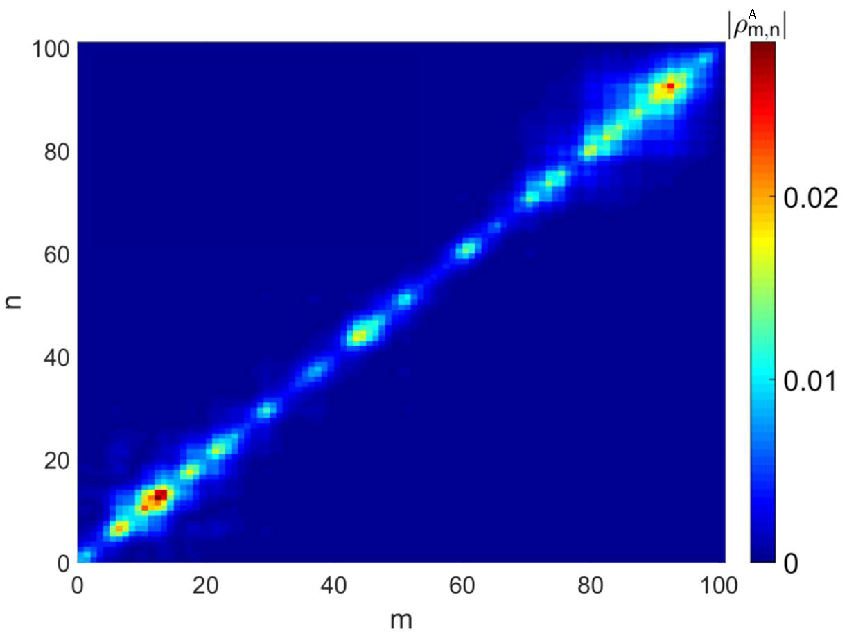
\includegraphics[width=0.5\linewidth]{anderson_rho_loc_1}}
		\hfill
		\subcaptionbox{\label{fig:anderson_rho_loc-2}}{%
			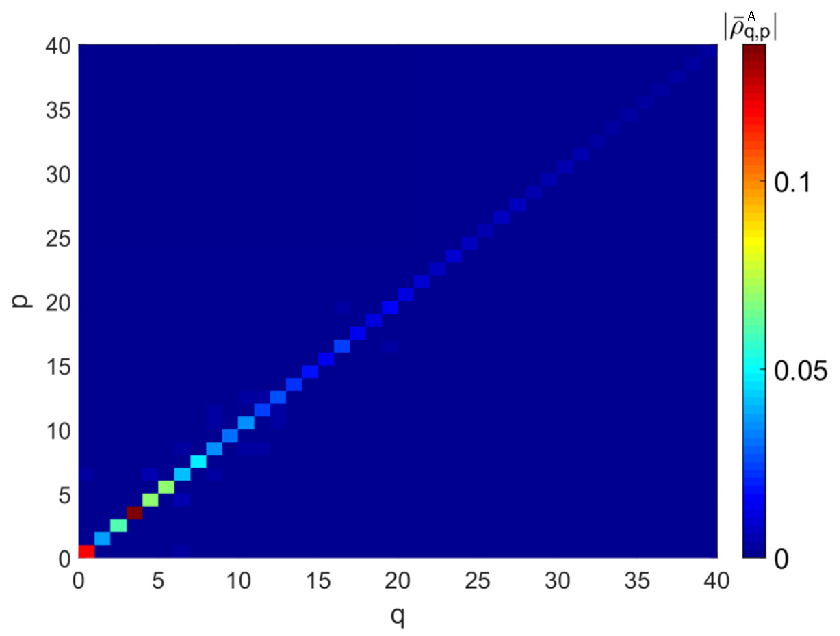
\includegraphics[width=0.5\linewidth]{anderson_rho_loc_2}}
		\hfill
	}
	\legend{}
	\caption[Этот текст попадает в названия рисунков в списке рисунков]
	{
		Абсолютные значения асимптотической матрицы плотности \(\rho^A\) в исходном базисе (a) и в базисе собственных состояний модели Андерсона (б) для единичной реализации беспорядка. Использовались неэрмитовые диссипаторы \cref{eq:anderson_diss_local} c параметрами \(\alpha=0\) и \(l=1\). Сила пространственного беспорядка \(W=1\).
	}
	\label{fig:anderson_rho_loc}
\end{figure}

Зафиксируем параметры диссипаторов \(\alpha=0\) и \(l=1\) в формуле \cref{eq:anderson_diss_local} (синфазная диссипация на соседних сайтах решётки). В этом случае асимптотическая матрица плотности \(\rho^A\) имеет пятнистую структуру с несколькими яркими областями локализации, как показано на рисунке~\cref{fig:anderson_rho_loc-1}.
Рассмотрим асимптотическую матрицу плотности \(\rho^A\) в базисе собственных состояний модели Андерсона:
\begin{equation}
\label{eq:anderson_rho_in_eigen_basis}
\begin{gathered}
\bar{\rho}^A = \mathcal{A}^\dagger \rho^A \mathcal{A},
\end{gathered}
\end{equation}
где \(\mathcal{A} = \left(A_1 \ldots A_\nu \ldots A_N \right) \) "--- матрица собственных векторов гамильтониана \cref{eq:anderson_H}. В данном представлении матрица плотности \(\bar{\rho}^A\) является практически диагональной, с большим преобладанием значений из нижней части спектра, как показано на рисунке~\cref{fig:anderson_rho_loc-2}.

Для аналитического подтверждения данного наблюдения перепишем уравнение \cref{eq:GKSL_base} в базисе собственных состояний модели Андерсона \cref{eq:anderson_rho_in_eigen_basis}, пренебрегая недиагональными элементами матрицы плотности. В таком приближении эволюция диагональных элементов определяется только диссипативными членами:
\begin{equation}
\label{eq:anderson_diag_mod_1}
\begin{gathered}
\dot{\bar{\rho}}_{p,p} = \gamma \left( \sum_q I_{p,q}\bar{\rho}_{q,q} - \bar{\rho}_{p,p} \sum_q I_{q,p} \right),
\end{gathered}
\end{equation}
где коэффициенты перекрытий \(I_{p,q}\) представляются следующим образом через диссипативные операторы в базисе собственных состояний модели Андерсона (\(\bar{V}_k = \mathcal{A}^\dagger V_k \mathcal{A}\)):
\begin{equation}
\label{eq:anderson_diag_mod_2}
\begin{gathered}
I_{p,q} = \sum_k \left| \left(\bar{V}_k\right)_{q,p} \right|^2 = \sum_k \left(\mathcal{A}_{p, k+l} + e^{i \alpha} \mathcal{A}_{p, k} \right)^2  \left(\mathcal{A}_{q, k+l} - e^{-i \alpha} \mathcal{A}_{q, k} \right)^2.
\end{gathered}
\end{equation}
Система линейных дифференциальных уравнений \cref{eq:anderson_diag_mod_1} имеет единственное устойчивое состояние равновесия. Для его поиска, приравняем правую часть уравнения к \(0\), введём переобозначение:
\begin{equation}
\label{eq:anderson_diag_mod_3}
\begin{gathered}
I^{\pm}_{p,k} = \left(\mathcal{A}_{p, k+l} \pm e^{\pm i \alpha} \mathcal{A}_{p, k} \right)^2 ,
\end{gathered}
\end{equation}
и получим итоговое выражение для асимптотического состояния равновесия:
\begin{equation}
\label{eq:anderson_diag_mod_4}
\begin{gathered}
\bar{\rho}^A_{p,p} = \frac{\sum_q I_{p,q}\bar{\rho}^A_{q,q}}{\sum_q I_{q,p}} = \frac{\sum_q \sum_k I^{+}_{p,k} I^{-}_{q,k} \bar{\rho}^A_{q,q}}{\sum_q \sum_k I^{+}_{q,k}  I^{-}_{p,k}} = \frac{\sum_k I^{+}_{p,k} \sum_q I^{-}_{q,k} \bar{\rho}^A_{q,q}}{ \sum_k I^{-}_{p,k} \sum_q  I^{+}_{q,k} } .
\end{gathered}
\end{equation}
Внутренние суммы в числителе и знаменателе в самой правой части выражения не зависят от индекса \(p\). Они подвергаются усреднению по всем охватываемым собственным состояниям. Поскольку беспорядок пространственно однороден, среднее по ансамблю делает результат также независимым от индекса \(k\), и поэтому обе суммы соответствуют некоторой нормировочной константе. Таким образом, мы приходим к следующему выражению для асимптотической матрицы плотности в базисе собственных состояний модели Андерсона:
\begin{equation}
\label{eq:anderson_diag_mod_5}
\begin{gathered}
\bar{\rho}^A_{p,p} \approx \frac{\sum_k I^{+}_{p,k}}{ \sum_k I^{-}_{p,k}}, 
\end{gathered}
\end{equation}
которое полностью определяется типом диссипации и пространственной структурой конкретного собственного состояния.

Для случая синфазной диссипации на соседних сайтах решётки (\(\alpha=0\) и \(l=1\) в \cref{eq:anderson_diss_local}) получается соотношение:
\begin{equation}
\label{eq:anderson_diag_mod_6}
\begin{gathered}
\sum_k \left( \mathcal{A}_{p, k+1} \pm \mathcal{A}_{p, k} \right)^2 = 2 \pm \sum_k \mathcal{A}_{p, k+1} \mathcal{A}_{p, k} = 2 \mp \lambda_p \mp \sum_k \varepsilon_k \mathcal{A}^2_{p, k}.
\end{gathered}
\end{equation}
Оно основано на тождестве, полученном из следующего уравнения для собственных состояний:
\begin{equation}
\label{eq:anderson_diag_mod_7}
\begin{gathered}
-\left( \lambda_p - \varepsilon_k \right) \mathcal{A}_{p, k} = \mathcal{A}_{p, k-1} + \mathcal{A}_{p, k+1},
\end{gathered}
\end{equation}
которое, в свою очередь, умножается на \(\mathcal{A}_{p, k}\) и суммируется по \(k\).
В уравнении \cref{eq:anderson_diag_mod_6} в случае малого беспорядка (\(W < 4\)) и далеко от границ спектра, можно пренебречь последним слагаемым в правой части (усреднение из-за пространственного беспорядка), и в итоге получить следующее соотношение:
\begin{equation}
\label{eq:anderson_diag_mod_8}
\begin{gathered}
\bar{\rho}^A_{p,p} \approx \frac{2-\lambda_p}{2+\lambda_p}.
\end{gathered}
\end{equation}
Данный результат объясняет быстрое уменьшение вклада собственных состояний при отдалении от нижней границы спектра.
На рисунке~\cref{fig:anderson_rho_nn_1} символами изображены усреднённые по многим реализация беспорядка распределения диагональных элементов асимптотической матрицы плотности в базисе собственных состояний модели Андерсона \(\bar{\rho}^A_{p,p}\) как функции усреднённых собственных значений для разных параметров силы беспорядка. Количество реализаций беспорядка для усреднения: \(M=100\).
Полученные численные результаты хорошо согласуются с теоретической оценкой (формула \cref{eq:anderson_diag_mod_8} и фиолетовая кривая на рисунке~\cref{fig:anderson_rho_nn_1}). 
Несоответствие между результатами численных экспериментов и теоретической оценкой увеличивается с ростом силы беспорядка \(W\) и вблизи границ спектра "--- эти эффекты следуют из природы сделанных приближений.
\begin{figure}[ht]
	\centerfloat{
		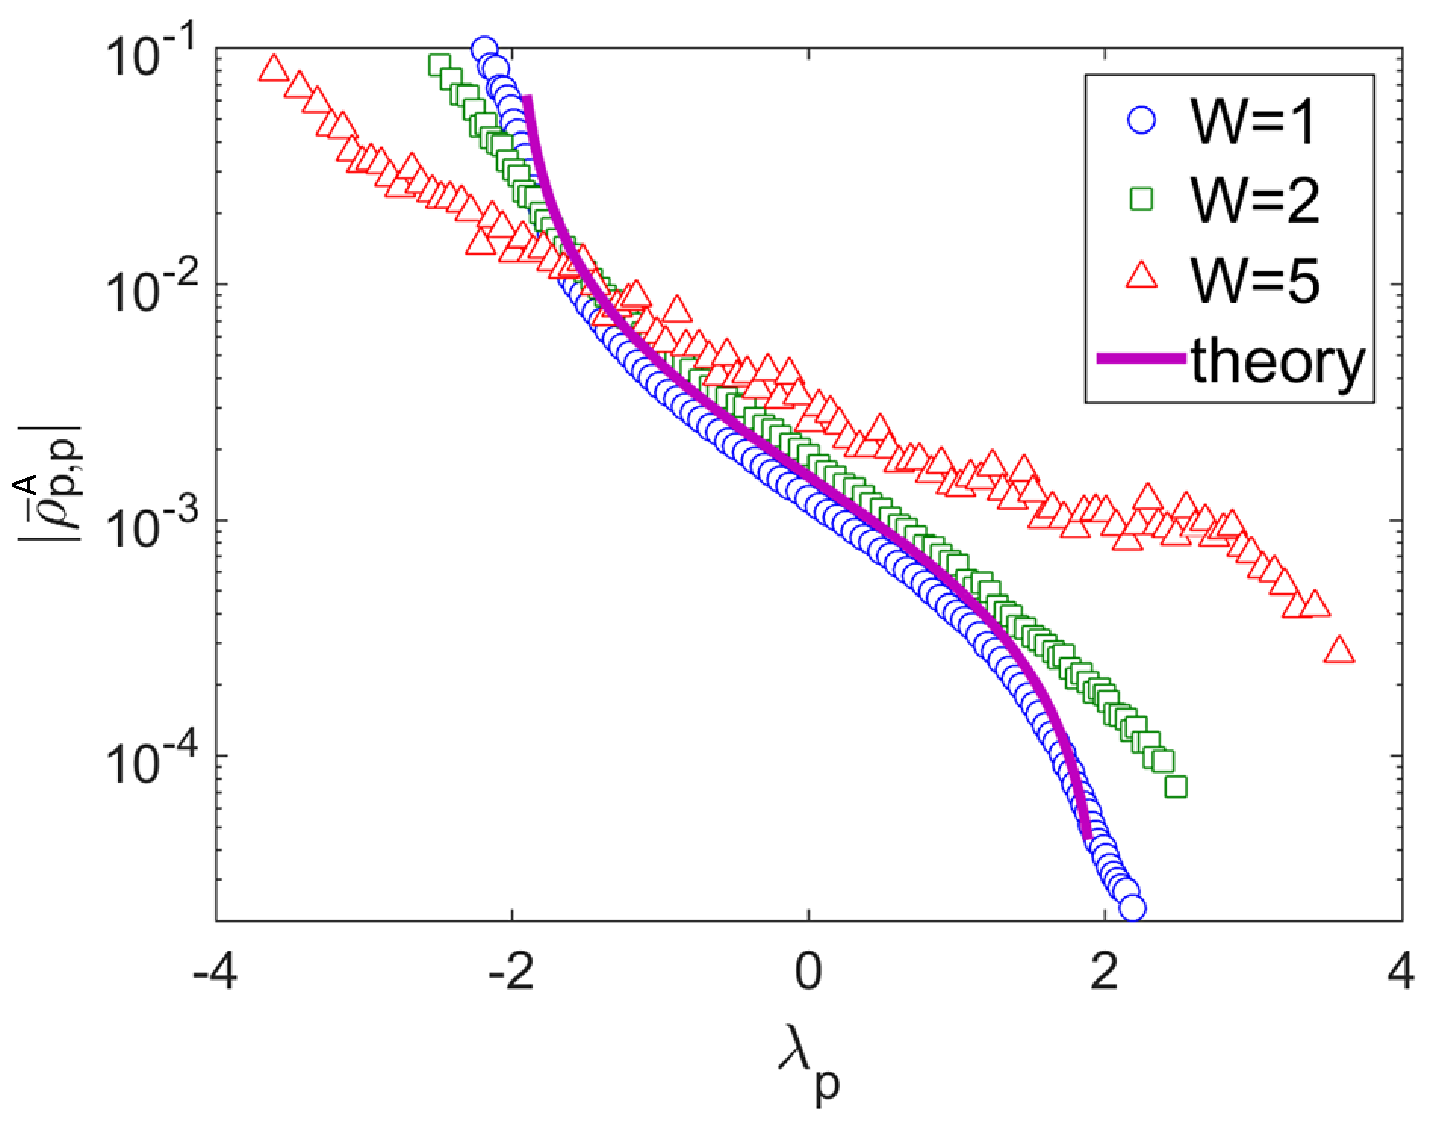
\includegraphics[scale=0.6]{anderson_rho_nn_1}
	}
	\caption{
		Символы "--- усреднённые абсолютные значения диагональных элементов асимптотической матрицы плотности в базисе собственных состояний модели Андерсона как функции усреднённых собственных чисел для синфазной диссипации на соседних сайтах решётки (\(\alpha=0\) и \(l=1\) в уравнении \cref{eq:anderson_diss_local}) для разных значений беспорядка \(W\). Теоретический результат (формула \cref{eq:anderson_diag_mod_8}) показан фиолетовой сплошной линией.
	}
	\label{fig:anderson_rho_nn_1}
\end{figure}

Случай антифазной диссипации на соседних сайтах решетки (\(\alpha=\pi\) и \(l=1\) в уравнении \cref{eq:anderson_diss_local}), из-за симметрии, приводит к обратному выражению для формулы \cref{eq:anderson_diag_mod_8}:
\begin{equation}
\label{eq:anderson_diag_mod_9}
\begin{gathered}
\bar{\rho}^A_{p,p} \approx \frac{2+\lambda_p}{2-\lambda_p}.
\end{gathered}
\end{equation}
Асимптотическая матрица плотности является локализованной возле верхней границы спектра. 
Если фазу диссипации взять равной \(\alpha=\frac{\pi}{2}\), то все диссипативные операторы \cref{eq:anderson_diss_local} окажутся эрмитовыми, что приведёт в итоге систему в тривиальное состояние с максимальной энтропией: \(\rho^A = \frac{\idmtx}{N}\).
При промежуточных значениях фазы диссипации \(0 < \alpha < \frac{\pi}{2}\) (\(\frac{\pi}{2} < \alpha < \pi\)) в асимптотической матрице плотности в базисе собственных состояний модели Андерсона будут преобладать диагональные элементы, локализованные вблизи нижней (верхней) границы спектра собственных значений.

Качественно иная картина наблюдается для диссипативных операторов с \(\alpha=\pi\) и \(l=2\).
В этом случае асимптотическая матрица плотности в исходном базисе \(\rho^A\) является относительно более делокализованной (рисунок~\cref{fig:anderson_rho_loc-3}). 
В то же время, в базисе собственных состояний модели Андерсона \(\bar{\rho}^A\) \cref{eq:anderson_rho_in_eigen_basis} остаётся локализованной со смещением в центр спектра (рисунок~\cref{fig:anderson_rho_loc-4}).
\begin{figure}[ht]
	\centerfloat{
		\hfill
		\subcaptionbox[List-of-Figures entry]{\label{fig:anderson_rho_loc-3}}{%
			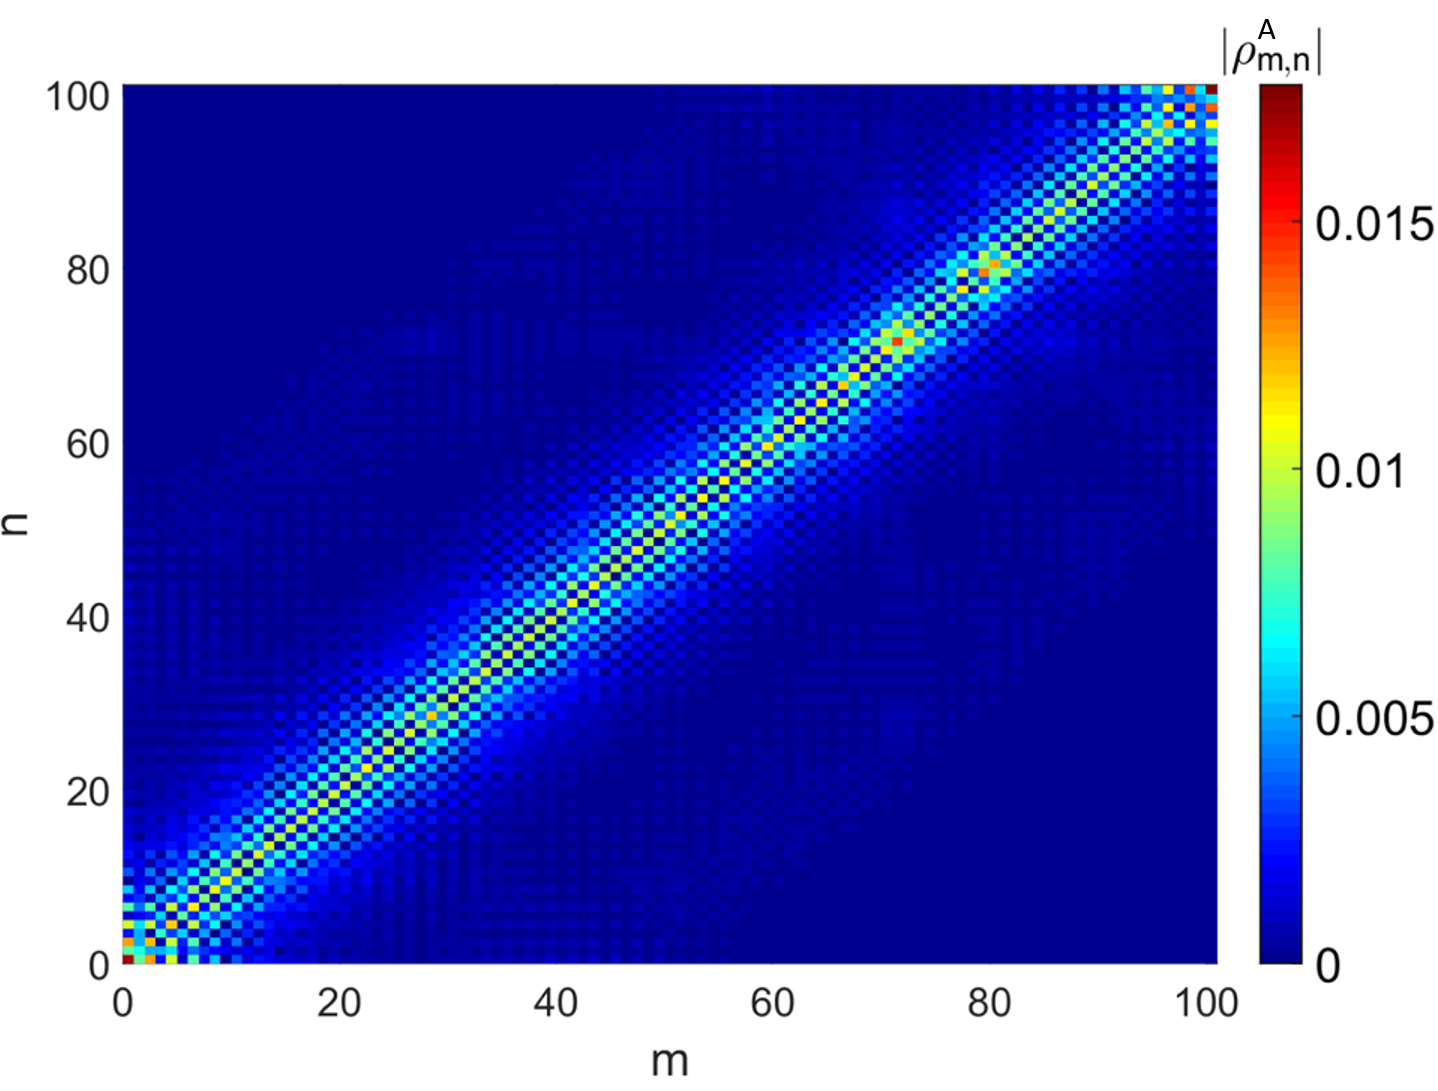
\includegraphics[width=0.5\linewidth]{anderson_rho_loc_3}}
		\hfill
		\subcaptionbox{\label{fig:anderson_rho_loc-4}}{%
			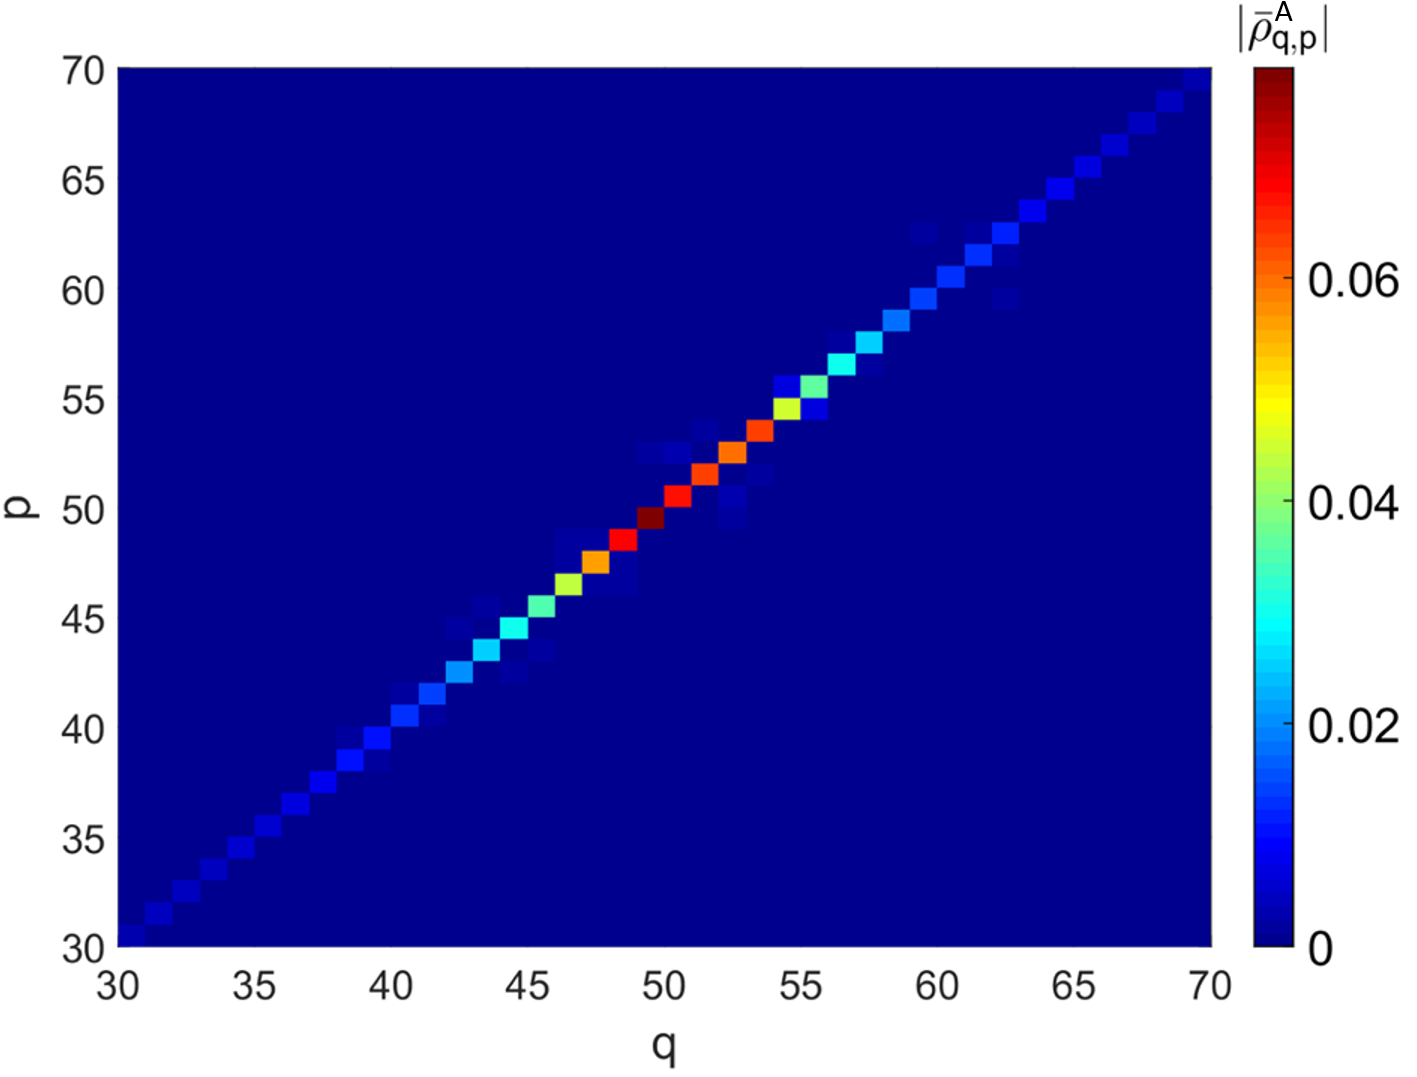
\includegraphics[width=0.5\linewidth]{anderson_rho_loc_4}}
		\hfill
	}
	\legend{}
	\caption[Этот текст попадает в названия рисунков в списке рисунков]
	{
		Абсолютные значения асимптотической матрицы плотности \(\rho^A\) в исходном базисе (a) и в базисе собственных состояний модели Андерсона (б) для единичной реализации беспорядка. Использовались неэрмитовые диссипаторы \cref{eq:anderson_diss_local} c параметрами \(\alpha=\pi\) и \(l=2\). Сила пространственного беспорядка \(W=1\).
	}
	\label{fig:anderson_rho_loc_mid}
\end{figure}
Относительная делокализация в исходном базисе вызвана существенным вкладом собственных состояний из центра спектра, которые имеют относительно большую длину локализации \cref{eq:anderson_loc_length}.
Аналитические соотношения для данного случая выглядят следующим образом:
\begin{equation}
\label{eq:anderson_diag_mod_10}
\begin{gathered}
I^{-}_p = \sum_{k} \left( \mathcal{A}_{p, k+2} \pm \mathcal{A}_{p, k} \right)^2 = \\
= \lambda^2 - 2 \lambda_p \sum_{k} \varepsilon_k \mathcal{A}_{p, k} \mathcal{A}_{p, k+1} + \sum_{k} \varepsilon^2_k \mathcal{A}^2_{p, k} \approx \lambda^2_p + \frac{W^2}{12}, \\
I^{+}_p = 4 - I^{-}_p,
\end{gathered}
\end{equation}
которые в итоге приводят к следующему выражению для диагональных элементов матрицы плотности в базисе собственных состояний модели Андерсона:
\begin{equation}
\label{eq:anderson_diag_mod_11}
\begin{gathered}
\bar{\rho}^A_{p,p} \approx \frac{4}{\lambda^2_p + \frac{W^2}{12}} - 1.
\end{gathered}
\end{equation}
Данное выражение указывает на то, что наибольший вклад в решение вносят собственные состояния из центра спектра.
На рисунке \cref{fig:anderson_rho_nn_2} изображены усреднённые по \(M=100\) случайным реализациям беспорядка диагональные элементы матрицы плотности в базисе собственных состояний модели Андерсона для разных значений силы беспорядка вместе с аналитическим результатом \cref {eq:anderson_diag_mod_11} (сплошные линии). На графике видно хорошее соответствие между численными и аналитическими результатами при малом беспорядке \(W\). При увеличении \(W\) несоответствие увеличивается на краях спектра \(\lambda_p\) ввиду сделанных теоретических приближений. 
\begin{figure}[ht]
	\centerfloat{
		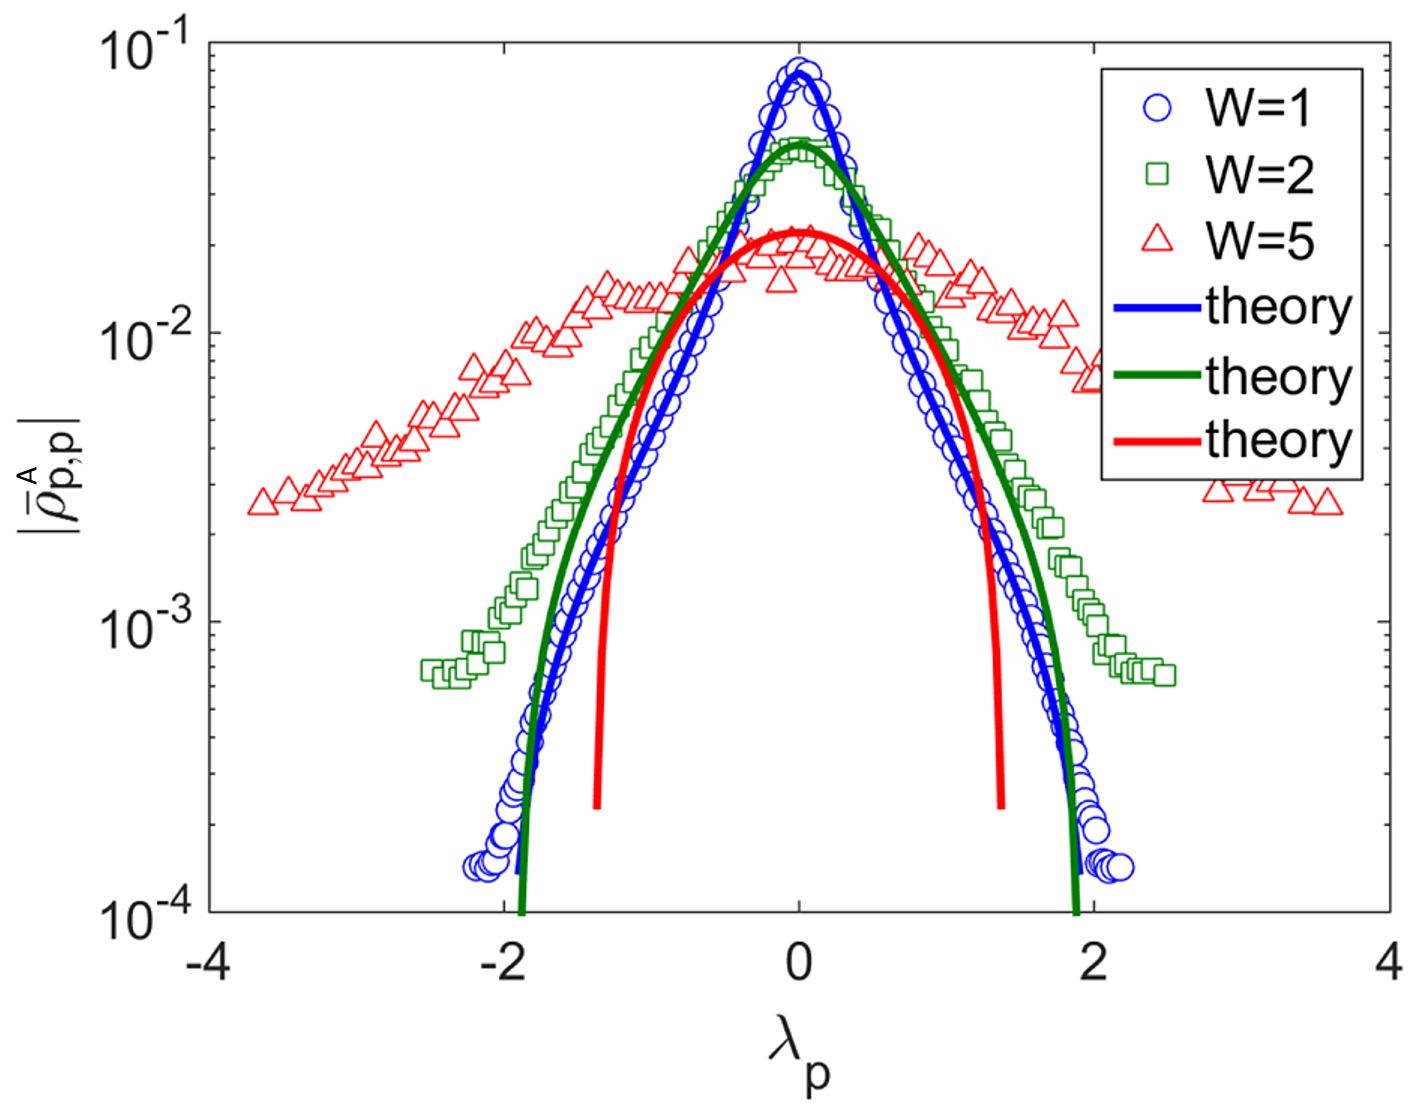
\includegraphics[scale=0.4]{anderson_rho_nn_2}
	}
	\caption{
		Символы "--- усреднённые абсолютные значения диагональных элементов асимптотической матрицы плотности в базисе собственных состояний модели Андерсона как функции усреднённых собственных чисел для синфазной диссипации на соседних сайтах решётки (\(\alpha=\pi\) и \(l=1\) в уравнении \cref{eq:anderson_diss_local}) для разных значений беспорядка \(W\). Теоретический результат (формула \cref{eq:anderson_diag_mod_11}) для каждого значения \(W\) показан соответствующей сплошной линией.
	}
	\label{fig:anderson_rho_nn_2}
\end{figure}

Рассмотрим открытую модель Андерсона \cref{eq:GKSL_lindbladian, eq:anderson_H, eq:anderson_diss_local} c микроскопической точки зрения, используя метод квантовых тректорий, описанный в разделе \cref{sec:ch1/sec2}. Квантовая траектория с индексом \(j\) будет описываться волновой функцией \(\left| \psi_j(t) \right\rangle\). Зафиксируем случайный беспорядок  силой \(W=1\) в системе и время переходного процесса \(t^A = 10^4\) "--- достаточным до достижения каждой траектории аттрактора (асимптотической матрицы плотности \(\rho^A\)). После достижения аттрактора за каждой квантовой траекторией будет вестись наблюдение в течении \(t^F = 10^4\) (суммарное время пропагации \(t = t^A + t^F\)). Количество рассматриваемых квантовых траекторий \(M_r=10^6\). Для каждой \(j\)-ой квантовой траектории будут рассматриваться позиция и энергия, вычисляемые по соответствующим формулам:
\begin{equation}
\label{eq:anderson_position}
\begin{gathered}
n_j(t) = \langle \psi_j(t)| O_n | \psi_j(t) \rangle,
\end{gathered}
\end{equation}
\begin{equation}
\label{eq:anderson_energy}
\begin{gathered}
E_j(t) = \langle \psi_j(t)| H | \psi_j(t) \rangle,
\end{gathered}
\end{equation}
где \(O_n\) - матрица оператора числа частиц, а \(H\) - гамильтониан модели Андерсона \cref{eq:anderson_H}.

\begin{figure}[ht]
	\centerfloat{
		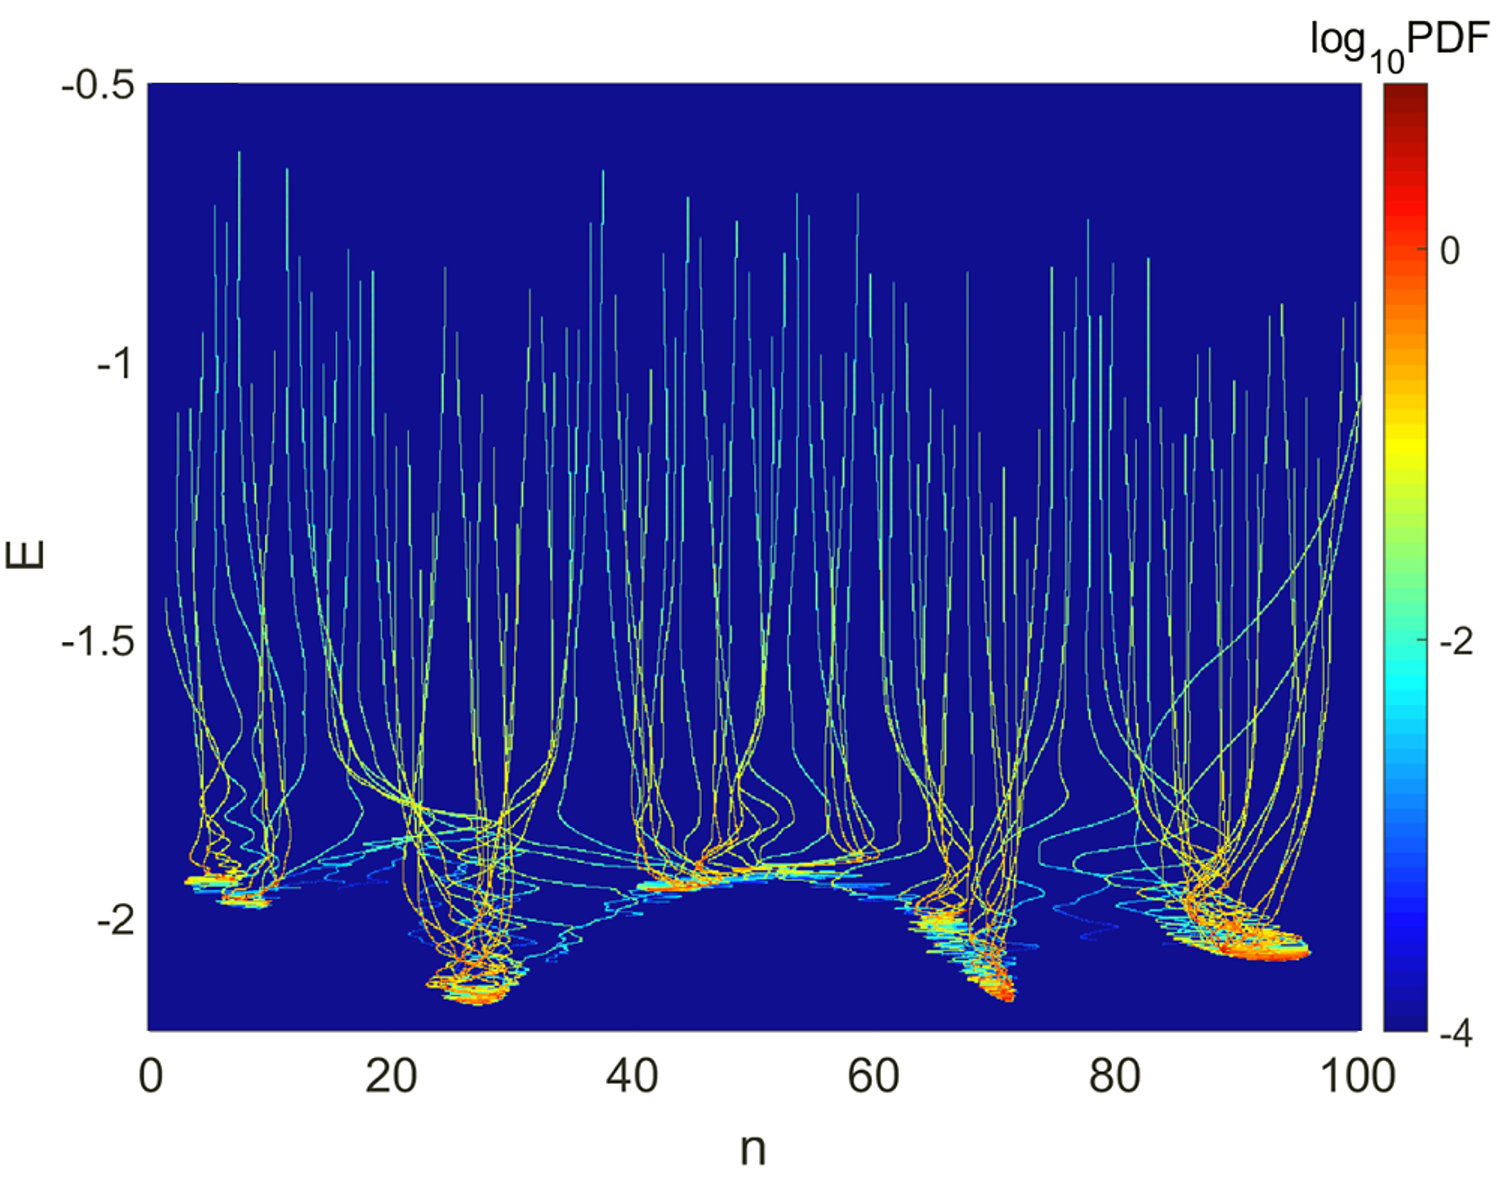
\includegraphics[scale=0.4]{anderson_qj_1}
	}
	\caption{
		Функция распределения плотности вероятностей (PDF) квантовых траекторий на плоскости позиции \(n(t)\) и энергии \(E(t))\) для случая синфазной диссипации на соседних сайтах решётки (\(\alpha=0\) и \(l=1\) в \cref{eq:anderson_diss_local}).
	}
	\label{fig:anderson_qj_1}
\end{figure}

На рисунке \cref{fig:anderson_qj_1} изображена двумерная функция распределения плотности вероятностей (probability densidy function - PDF) на плоскости позиции \(n(t)\) \cref{eq:anderson_position} и энергии \(E(t)\) \cref{eq:anderson_energy} , построенная для \(M_r=10^6\) траекторий, наблюдаемых в течение \(t^F=10^4\) времени для случая синфазной диссипации на соседних сайтах решётки (\(\alpha=0\) и \(l=1\) в \cref{eq:anderson_diss_local}). Динамика отдельных квантовых траекторий представляет собой длительные «залипания» вблизи центров локализации (красные области на рисунке \cref{fig:anderson_qj_1}), вызванные эволюцией с неэрмитовым гамильтонианом \cref{eq:H_nonhermit} (алгоритм \ref{alg:qt_main}). Данные процессы прерываются квантовыми скачками (алгоритм \ref{alg:qt_jump}), которые накачивают систему энергией и переносят траектории в бледно-голубые «истоки» сети в верхней части рисунка \cref{fig:anderson_qj_1}, откуда системы быстро релаксирует по структурированной сети к одному из собственных состояний модели Андерсона. Структура сети не меняется при дальнейшем увеличении числа траекторий \(M_r\).

Результаты \cite{Yusipov2017}, представленные в данном разделе, указывают на то, что в открытых квантовых системах с физически реализуемой диссипацией возможно создание стационарных состояний, которые доминируют несколько локализованных мод пространственно неоднородного гамильтониана из классической модели Андерсона. Андерсоновские моды выбираются в соответствии с их пространственно-фазовыми свойствами, унаследованными от собственных состояний гамильтониана в пределе нулевого беспорядка \cite{Ishii1973}, с использованием фазо-параметризованных диссипативных операторов. Изменение фазы диссипативных операторов изменяет локализационные свойства системы.
 
\section{Управление одночастичной локализацией в открытых квантовых системах}\label{sec:ch1/epjb}
В данном разделе будет изучено влияние параметров диссипативных операторов \cref{eq:anderson_diss_local} на локализационные свойства открытой квантовой системы \cref{eq:GKSL_lindbladian,eq:anderson_H}, а также влияние добавочной дефазирующей диссипации \cref{eq:anderson_diss_dephase} на асимптотическое состояние системы.

Рассмотрим случай синфазной диссипации на соседних сайтах решётки (\(\alpha=0\) и \(l=1\) в \cref{eq:anderson_diss_local} с коэффициентами скорости диссипации \(\gamma^l = 0.1\). Добавим к данной модели дополнительные дефазирующие \cref{eq:anderson_diss_dephase} каналы рассеивания с коэффициентами скорости \(\gamma^d\). На рисунке \cref{fig:anderson_rho_nn_with_dephasing} изображены диагональные элементы асимптотической матрицы плотности в базисе собственных состояний модели Андерсона со смешанным типом диссипации для разных значений \(\gamma^d\). Стоить отметить, что не только слабая \(\gamma^d \ll \gamma^l\), но и сильная \(\gamma^d \gg \gamma^l\) дефазирующая диссипация не уничтожает спектральную диссипацию и структурно не изменяет решение (преобладают собственные состояния из той же части спектра).

\begin{figure}[ht]
	\centerfloat{
		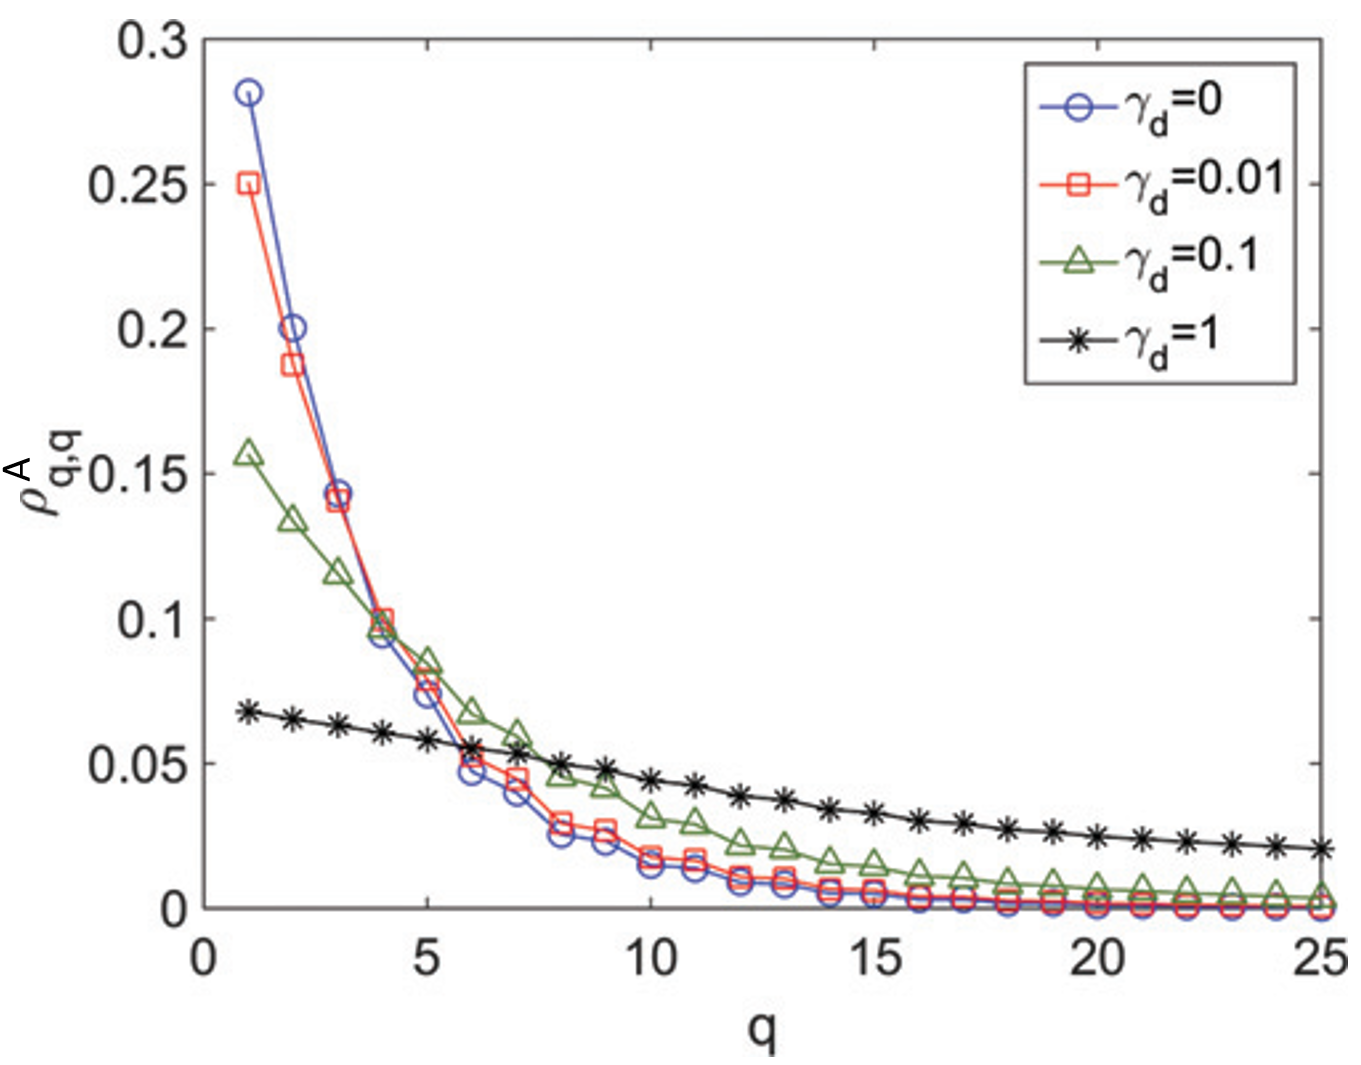
\includegraphics[scale=0.4]{anderson_rho_nn_with_dephasing}
	}
	\caption{
		Диагональные элементы асимптотической матрицы плотности в базисе собственных состояний модели Андерсона \(\bar{\rho}^A\) для случая синфазной диссипации на соседних сайтах решётки (\(\alpha=0\) и \(l=1\) в \cref{eq:anderson_diss_local} и скорость диссипации \(\gamma^l=0.1\)) в комбинации с дефазирующей диссипацией (\cref{eq:anderson_diss_dephase} и скорость диссипации \(\gamma^d\)) для разных значений \(\gamma^d\). Размер системы \(N=25\), сила пространственного беспорядка \(W=2\). Усреднение производилось для \(N_r = 10^3\) реализаций беспорядка. 
	}
	\label{fig:anderson_rho_nn_with_dephasing}
\end{figure}

Рассмотрим теперь систему в пределе нулевого беспорядка. Базис системы состоит из плоских волн с соответсвующим спектром собственных значений:
\begin{equation}
\label{eq:anderson_plane_wave}
\begin{gathered}
\phi_j = \frac{e^{i j k}}{\sqrt{N}}, \\
\lambda_k = -2 \cos{k}, \\
k = \frac{2 \pi q}{N}, \\
q = -\frac{N}{2}, \ldots, \frac{N}{2}.
\end{gathered}
\end{equation}
Можно заметить, что для конкретного значения фазы диссипатора \cref{eq:anderson_diss_local} \(\alpha = \frac{2 \pi q}{N}\), плоская  \cref{eq:anderson_plane_wave} с соответствующим \(k=\alpha\) является «тёмным» состоянием для всех диссипативных операторов \cref{eq:anderson_diss_local} \cite{Diehl2008, Kraus2008}, в то время как все остальные собственные состояния не являются.
В этом случае (когда нет дефазирующей добавки \(\gamma^d = 0\)), плоская волна с \(k = \alpha\) является асимптотическим состоянием открытой квантовой системы. 
В том случае, когда \(\alpha\) не совпадает точно со значением \(k\) или присутствует дефазирующая диссипация, асимптотическое состояние остаётся очень близким к исходному «тёмному» состоянию, причём наибольший вклад вносят плоские волны с \(k \approx \alpha\) (рисунок \cref{fig:anderson_rho_nn_zero_disorder}).
\begin{figure}[ht]
	\centerfloat{
		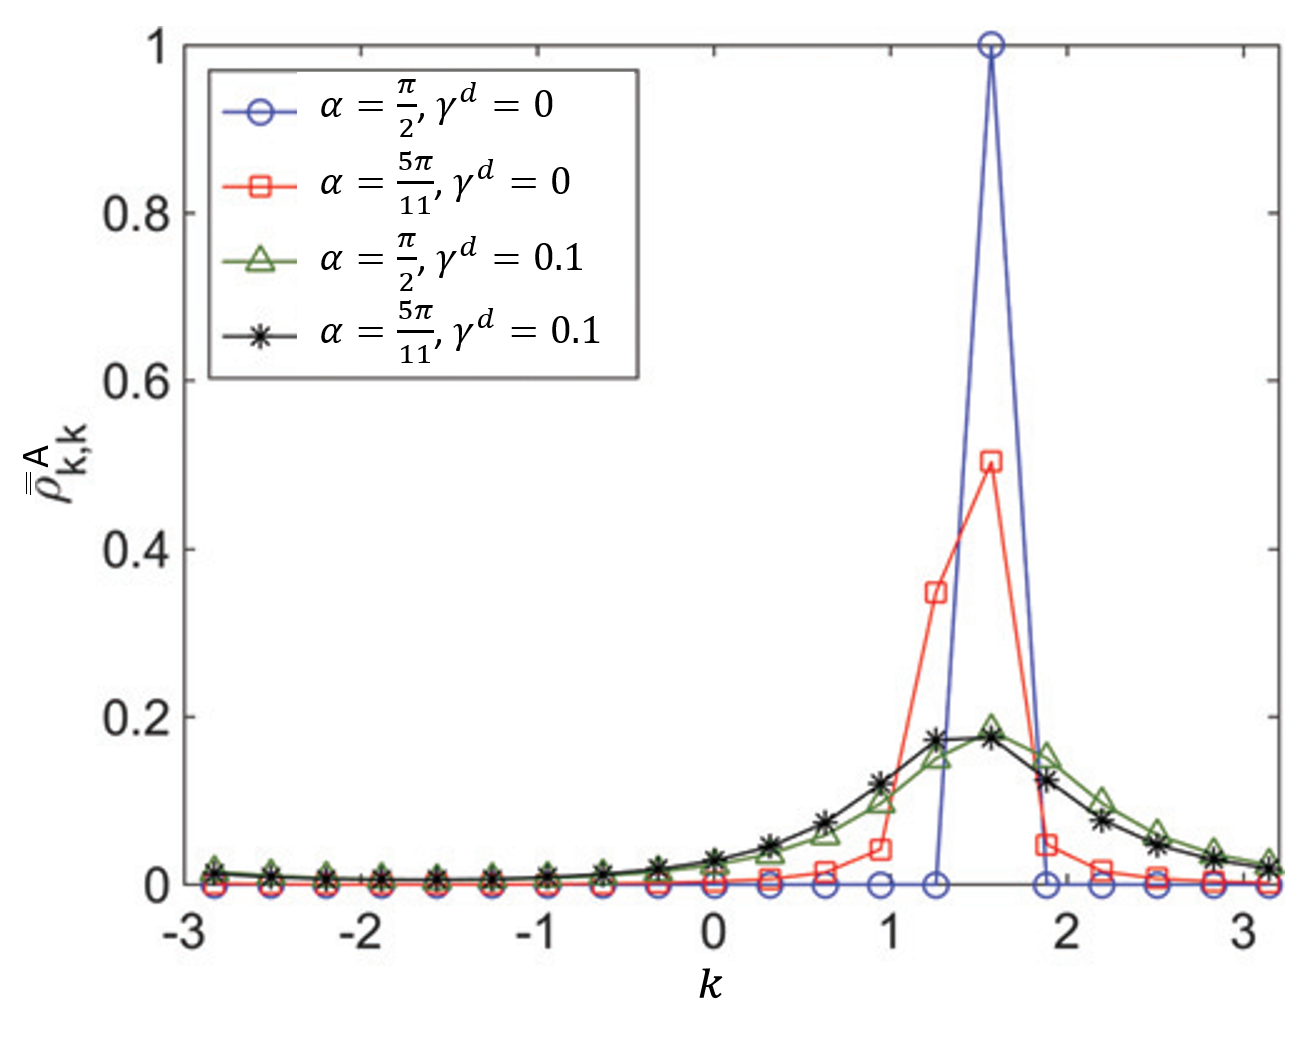
\includegraphics[scale=0.4]{anderson_rho_nn_zero_disorder}
	}
	\caption{
		Диагональные элементы асимптотической матрицы плотности в базисе плоских волн \(\bar{\bar{\rho}}^A_{k,k}\) \cref{eq:anderson_plane_wave} для случая синфазной диссипации на соседних сайтах решётки (\(\alpha=0\) и \(l=1\) в \cref{eq:anderson_diss_local} и скорость диссипации \(\gamma^l=0.1\)) в комбинации с дефазирующей диссипацией (\cref{eq:anderson_diss_dephase} и скорость диссипации \(\gamma^d\)). Размер системы \(N=20\), сила пространственного беспорядка \(W=0\).
	}
	\label{fig:anderson_rho_nn_zero_disorder}
\end{figure}

Ненулевой беспорядок \(W\) приводит к локализации Андерсона всех собственных состояний данной модели, которые при этом перестают в точности быть «тёмными» состояниями соответствующих диссипаторов \cref{eq:anderson_diss_local}.
Однако, известно, что моды Андерсона наследуют фазовые свойства исходных плоских волн (по крайней мере, в режиме слабого беспорядка), хотя их амплитуды экспоненциально затухают в пространстве \cite{Ishii1973}.
Следовательно, избирательный эффект локальных диссипаторов сохраняется.
\begin{figure}[h]
	\centerfloat{
		\hfill
		\subcaptionbox[List-of-Figures entry]{\label{fig:anderson_modes_in_foutier_1_1}}{%
			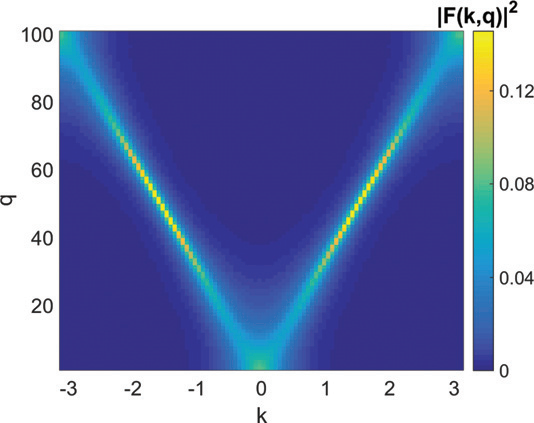
\includegraphics[width=0.45\linewidth]{anderson_modes_in_fourier_1_1}}
		\hfill
		\subcaptionbox{\label{fig:anderson_modes_in_foutier_1_2}}{%
			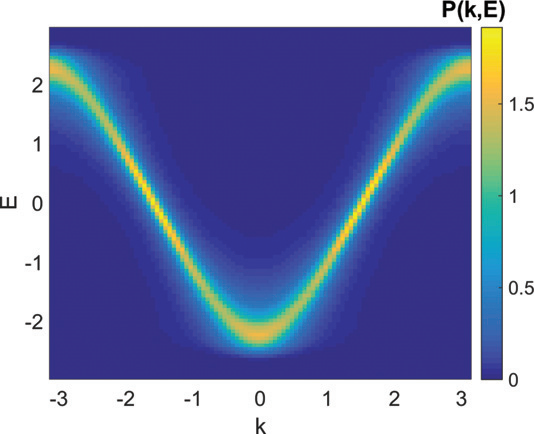
\includegraphics[width=0.45\linewidth]{anderson_modes_in_fourier_1_2}}
		\hfill
	}
	\legend{}
	\caption[Этот текст попадает в названия рисунков в списке рисунков]
	{
		Собственные состояния модели Андерсона (Андерсоновские моды) с беспорядком \(W=2\) в Фурье"--~базисе плоских волн \cref{eq:anderson_modes_in_plane_wave}. (а): квадрат значения гармоник \(\left| F(k,q) \right|^2\) в зависимости от волнового числа \(k\) и номера моды \(q\); (б): значения спектральной плотности \(P(k,E)\) \cref{eq:anderson_modes_in_plane_wave_density}.
	}
	\label{fig:anderson_modes_in_foutier_1}
\end{figure}
\begin{figure}[h]
	\centerfloat{
		\hfill
		\subcaptionbox[List-of-Figures entry]{\label{fig:anderson_modes_in_foutier_2_1}}{%
			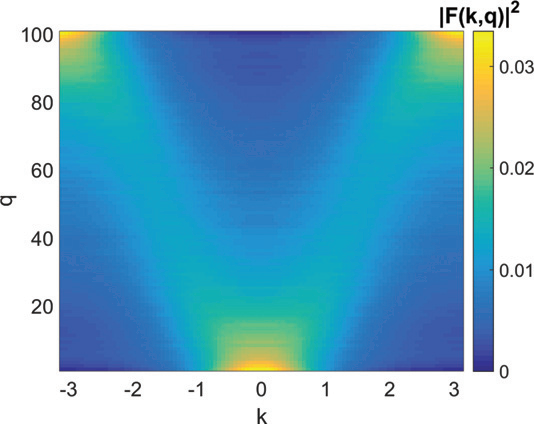
\includegraphics[width=0.45\linewidth]{anderson_modes_in_fourier_2_1}}
		\hfill
		\subcaptionbox{\label{fig:anderson_modes_in_foutier_2_2}}{%
			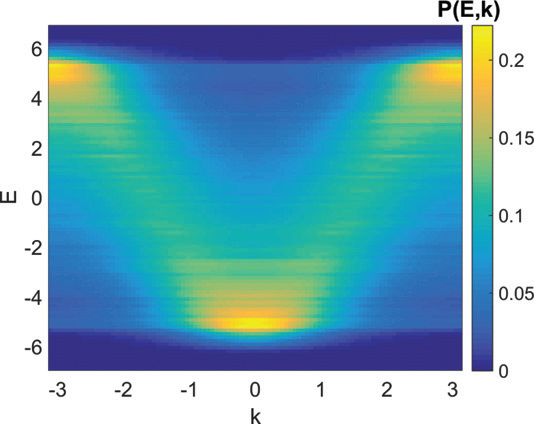
\includegraphics[width=0.45\linewidth]{anderson_modes_in_fourier_2_2}}
		\hfill
	}
	\legend{}
	\caption[Этот текст попадает в названия рисунков в списке рисунков]
	{
		Собственные состояния модели Андерсона (Андерсоновские моды) с беспорядком \(W=10\) в Фурье"--~базисе плоских волн \cref{eq:anderson_modes_in_plane_wave}. (а): квадрат значения гармоник \(\left| F(k,q) \right|^2\) в зависимости от волнового числа \(k\) и номера моды \(q\); (б): значения спектральной плотности \(P(k,E)\) \cref{eq:anderson_modes_in_plane_wave_density}.
	}
	\label{fig:anderson_modes_in_foutier_2}
\end{figure}
\begin{figure}[h]
	\centerfloat{
		\hfill
		\subcaptionbox[List-of-Figures entry]{\label{fig:anderson_rho_kk_in_foutier_1_1}}{%
			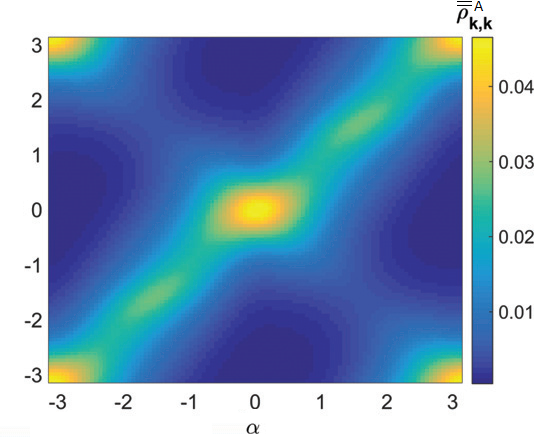
\includegraphics[width=0.45\linewidth]{anderson_rho_kk_in_foutier_1_1}}
		\hfill
		\subcaptionbox{\label{fig:anderson_rho_kk_in_foutier_1_2}}{%
			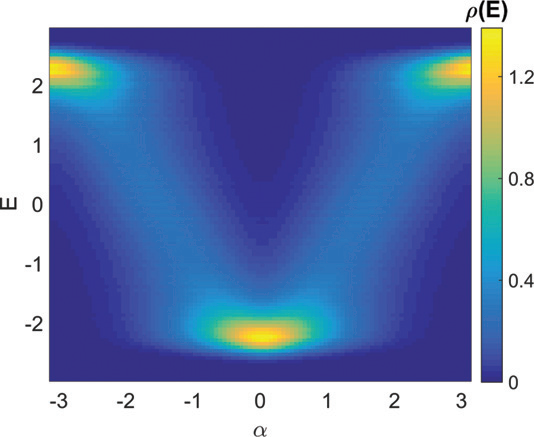
\includegraphics[width=0.45\linewidth]{anderson_rho_kk_in_foutier_1_2}}
	}
	\legend{}
	\caption[Этот текст попадает в названия рисунков в списке рисунков]
	{
		Асимптотическое состояние открытой системы Андерсона с беспорядком \(W=2\) и усреднением по \(N_r=10^3\) реализаций беспорядка в зависимости от параметра диссипации \(\alpha\) (\cref{eq:anderson_diss_local}). (а): диагональные элементы асимптотической матрицы плотности в базисе плоских волн \(\rho^A_{k,k}\) \cref{eq:anderson_plane_wave} ; (б): спектральная плотность диагональных элементов матрицы плотности в базисе собственных состояний модели Андерсона.
	}
	\label{fig:anderson_rho_kk_in_foutier_1}
\end{figure}
\begin{figure}[h]
	\centerfloat{
		\hfill
		\subcaptionbox[List-of-Figures entry]{\label{fig:anderson_rho_kk_in_foutier_2_1}}{%
			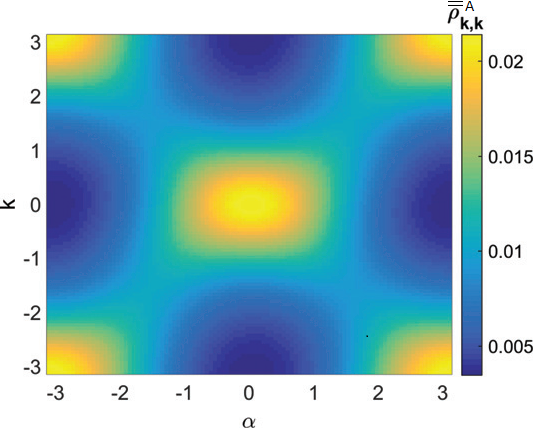
\includegraphics[width=0.45\linewidth]{anderson_rho_kk_in_foutier_2_1}}
		\hfill
		\subcaptionbox{\label{fig:anderson_rho_kk_in_foutier_2_2}}{%
			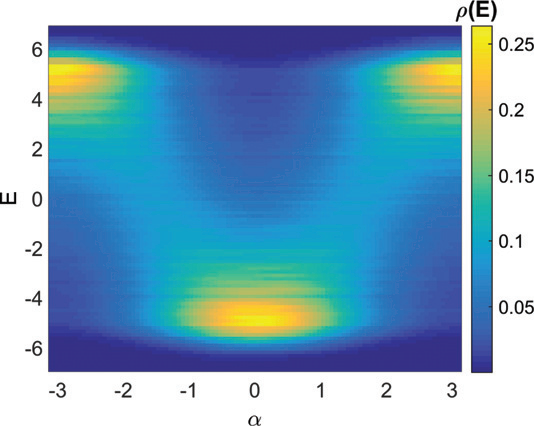
\includegraphics[width=0.45\linewidth]{anderson_rho_kk_in_foutier_2_2}}
	}
	\legend{}
	\caption[Этот текст попадает в названия рисунков в списке рисунков]
	{
		Асимптотическое состояние открытой системы Андерсона с беспорядком \(W=10\) и усреднением по \(N_r=10^3\) реализаций беспорядка в зависимости от параметра диссипации \(\alpha\) (\cref{eq:anderson_diss_local}). (а): диагональные элементы асимптотической матрицы плотности в базисе плоских волн \(\rho^A_{k,k}\) \cref{eq:anderson_plane_wave} ; (б): спектральная плотность диагональных элементов матрицы плотности в базисе собственных состояний модели Андерсона.
	}
	\label{fig:anderson_rho_kk_in_foutier_2}
\end{figure}

Зафиксируем параметры системы \(\gamma^l = \gamma^d = 0.1\), \(N=100\) и проанализируем структуру Андерсоновских мод \(A^{q}_k\) в базисе плоских волн \cref{eq:anderson_plane_wave} (Фурье"--~базис) для разных значений силы беспорядка \(W\).
Несмотря на то, что экспоненциальная локализация в прямом пространстве предполагает делокализацию в базисе плоских волн, она не исключает неоднородности распределения в нем.
Коэффициенты разложения, которые выражаются следующим образом:
\begin{equation}
\label{eq:anderson_modes_in_plane_wave}
\begin{gathered}
F(k,q) = \sum A^q_k \frac{e^{i j k}}{\sqrt{N}},
\end{gathered}
\end{equation}
имеют ярко выраженные максимумы вдоль линейных зависимостей \(q \approx \pm k_{max}\), как показано на рисунке \cref{fig:anderson_modes_in_foutier_1_1}.
Также была вычислена спектральная плотность коэффициентов разложения:
\begin{equation}
\label{eq:anderson_modes_in_plane_wave_density}
\begin{gathered}
P(k,E) = \lim_{\Delta E \to 0} \frac{1}{\Delta E} \sum_{q:E(q) \in [E, E + \Delta E]} \left| F(k,q) \right|^2 ,
\end{gathered}
\end{equation}
которая воспроизводит дисперсионное соотношение (рисунок \cref{fig:anderson_modes_in_foutier_1_2}).
Примечательно, что эти особенности присутствуют даже в режиме сильного беспорядка \(W=10\) (рисунок \cref{fig:anderson_modes_in_foutier_2_1, fig:anderson_modes_in_foutier_2_2}).

Связь между пространственной структурой мод Андерсона и их положением в спектре даёт ключ к пониманию способа выбора мод для формирования асимптотического состояния. Очевидно, это можно сделать, варьируя фазовый параметр \(\alpha\) локальных диссипаторов \cref{eq:anderson_diss_local}.
Численные результаты показывают хорошо очерченный максимум диагональных элементов асимптотической матрицы плотности в базисе плоских волн \(\bar{\bar{\rho}}^A_{k,k}\), такой, что \(k_{max} \approx \alpha\) (рисунок \cref{fig:anderson_rho_kk_in_foutier_1_1}). Также была вычислена спектральная плотность диагональных элементов матрицы плотности в базисе собственных состояний модели Андерсона \cref{eq:anderson_rho_in_eigen_basis}:
\begin{equation}
\label{eq:anderson_rho_kk_density}
\begin{gathered}
\varrho(E) = \lim_{\Delta E \to 0} \frac{1}{\Delta E} \sum_{q:E(q) \in [E, E + \Delta E]} \bar{\rho}^A_{q,q},
\end{gathered}
\end{equation}
проиллюстрированная на рисунке \cref{fig:anderson_rho_kk_in_foutier_1}. Точно так же, хотя и с менее чёткими границами воспроизводятся все результаты для случая сильного беспорядка \(W=10\) (рисунок \cref{fig:anderson_rho_kk_in_foutier_2}).

Таким образом, было продемонстрировано, что синтетическая диссипация может использоваться для управления свойствами локализации асимптотических состояний одночастичных квантовых систем. Механизм управления основан на фазовых свойствах локализованных мод гамильтониана системы Андерсона, которые являются  «тёмными» (либо близкими к «тёмным») состояниями синтетических диссипаторов \cite{Vershinina2017}.

\section{Распространение волновых пакетов в открытых квантовых системах с локализацией}\label{sec:ch1/prb_jump}
В данном разделе изучаются режимы распространения волновых пакетов квантовых траекторий \cite{Dalibard1992, Dum1992, Plenio1998} (раздел \cref{sec:ch1/sec2}) в открытой модели Андерсона (раздел \cref{sec:ch1/sec3}). Также будет рассмотрена статистика времён между последовательными квантовыми скачками для разных режимов распространения.

Зафиксируем общий случай параметров модели в рамках данного раздела (если нет дополнительных уточнений): размер системы \(N=200\), количество квантовых траекторий для усреднения \(M_r=10^3\), сила пространственного беспорядка \(W=1\), время переходного процесса для достижения аттрактора \(t^A = \frac{10^3}{\gamma}\), общее время интегрирования \(t^A + t^F = 10^7\) и периодические граничные условия \(\rho_0 = \rho_{N+1}\). Используются локальные диссипаторы \cref{eq:anderson_diss_local} с разными значениями фазы \(\alpha\) и, как контрольный случай, дефазирующие диссипаторы \cref{eq:anderson_diss_dephase}.

Асимптотическая матрица плотности \(\rho^A\) описывает статистическое распределение единичных квантовых траекторий, но не содержит информации о микроскопической динамике в асимптотическом режиме. Для данного типа анализа применяется метод квантовых траекторий, описанный в разделе \cref{sec:ch1/sec2}.

\begin{figure}[ht]
	\centerfloat{
		\hfill
		\subcaptionbox[List-of-Figures entry]{\label{fig:anderson_prb_1_1}}{%
			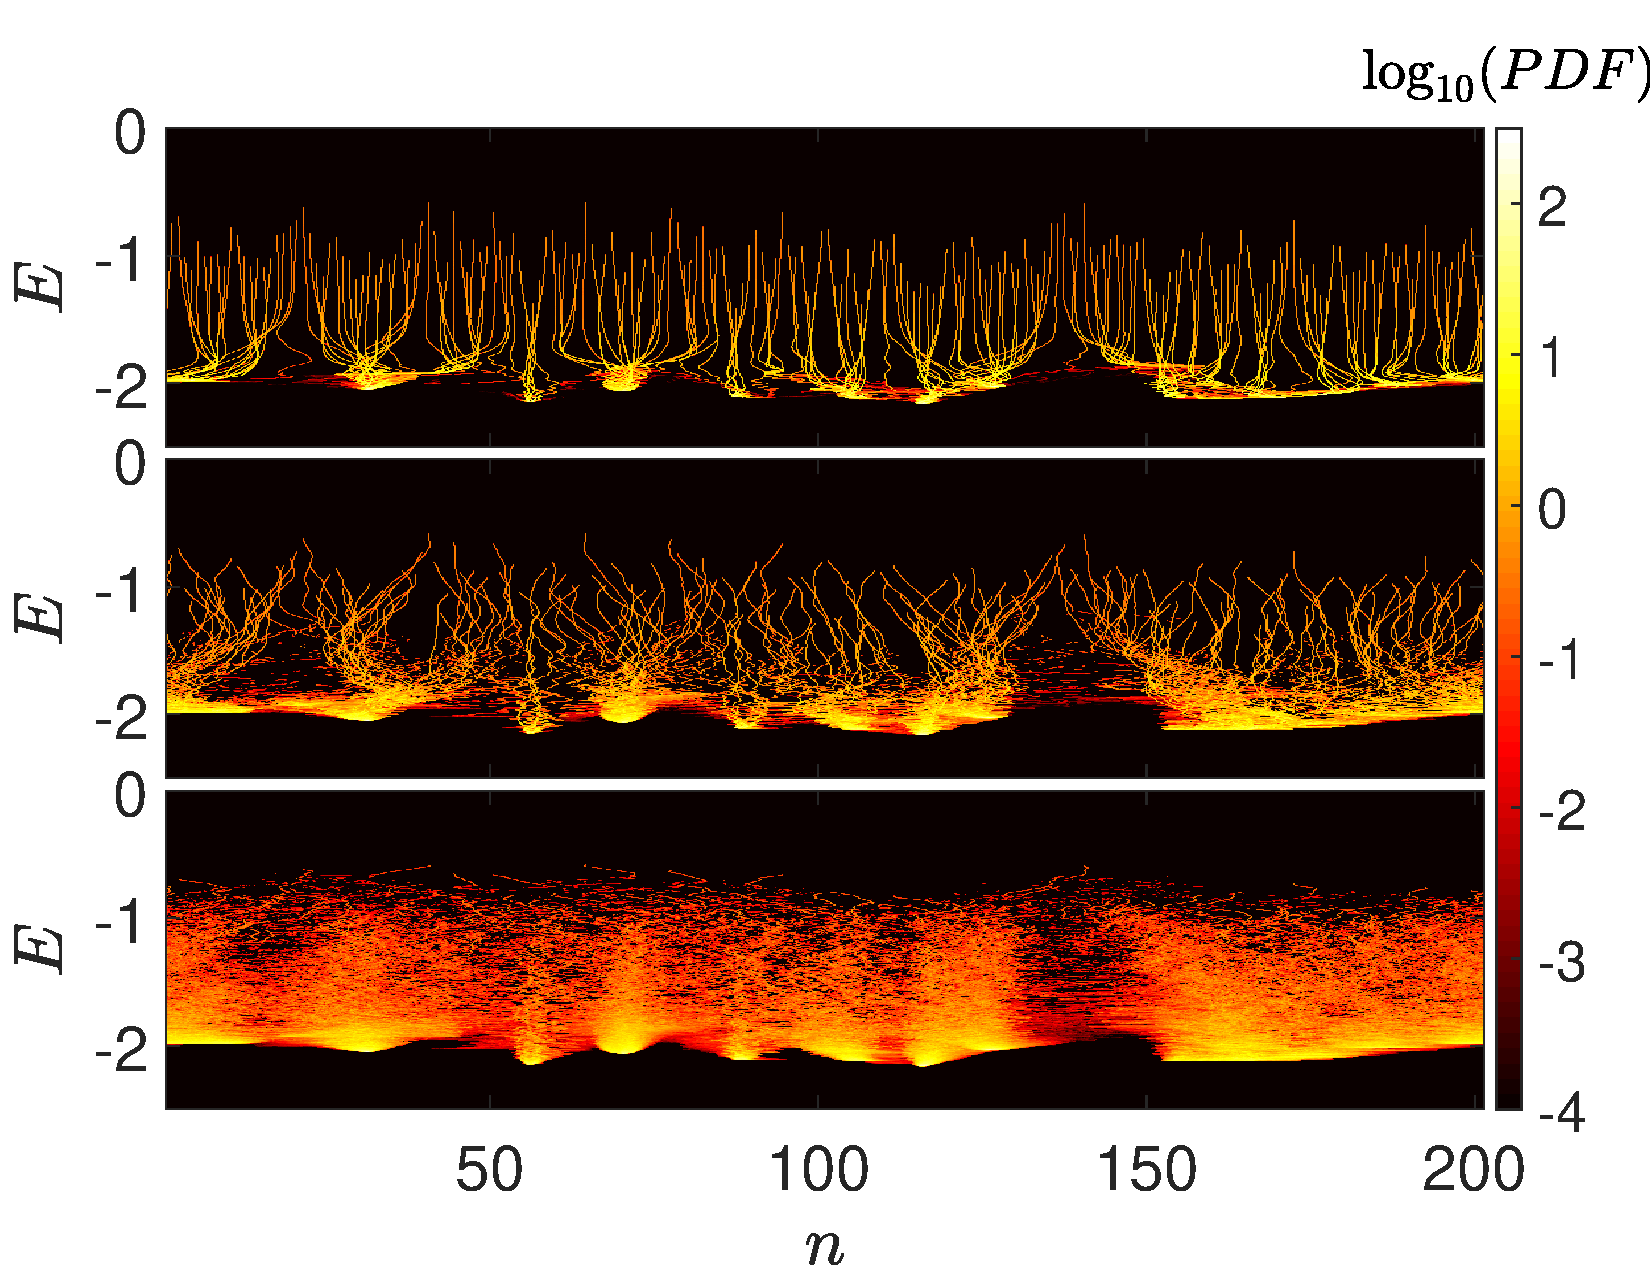
\includegraphics[width=0.5\linewidth]{anderson_prb_1_1}}
		\hfill
		\subcaptionbox{\label{fig:anderson_prb_1_2}}{%
			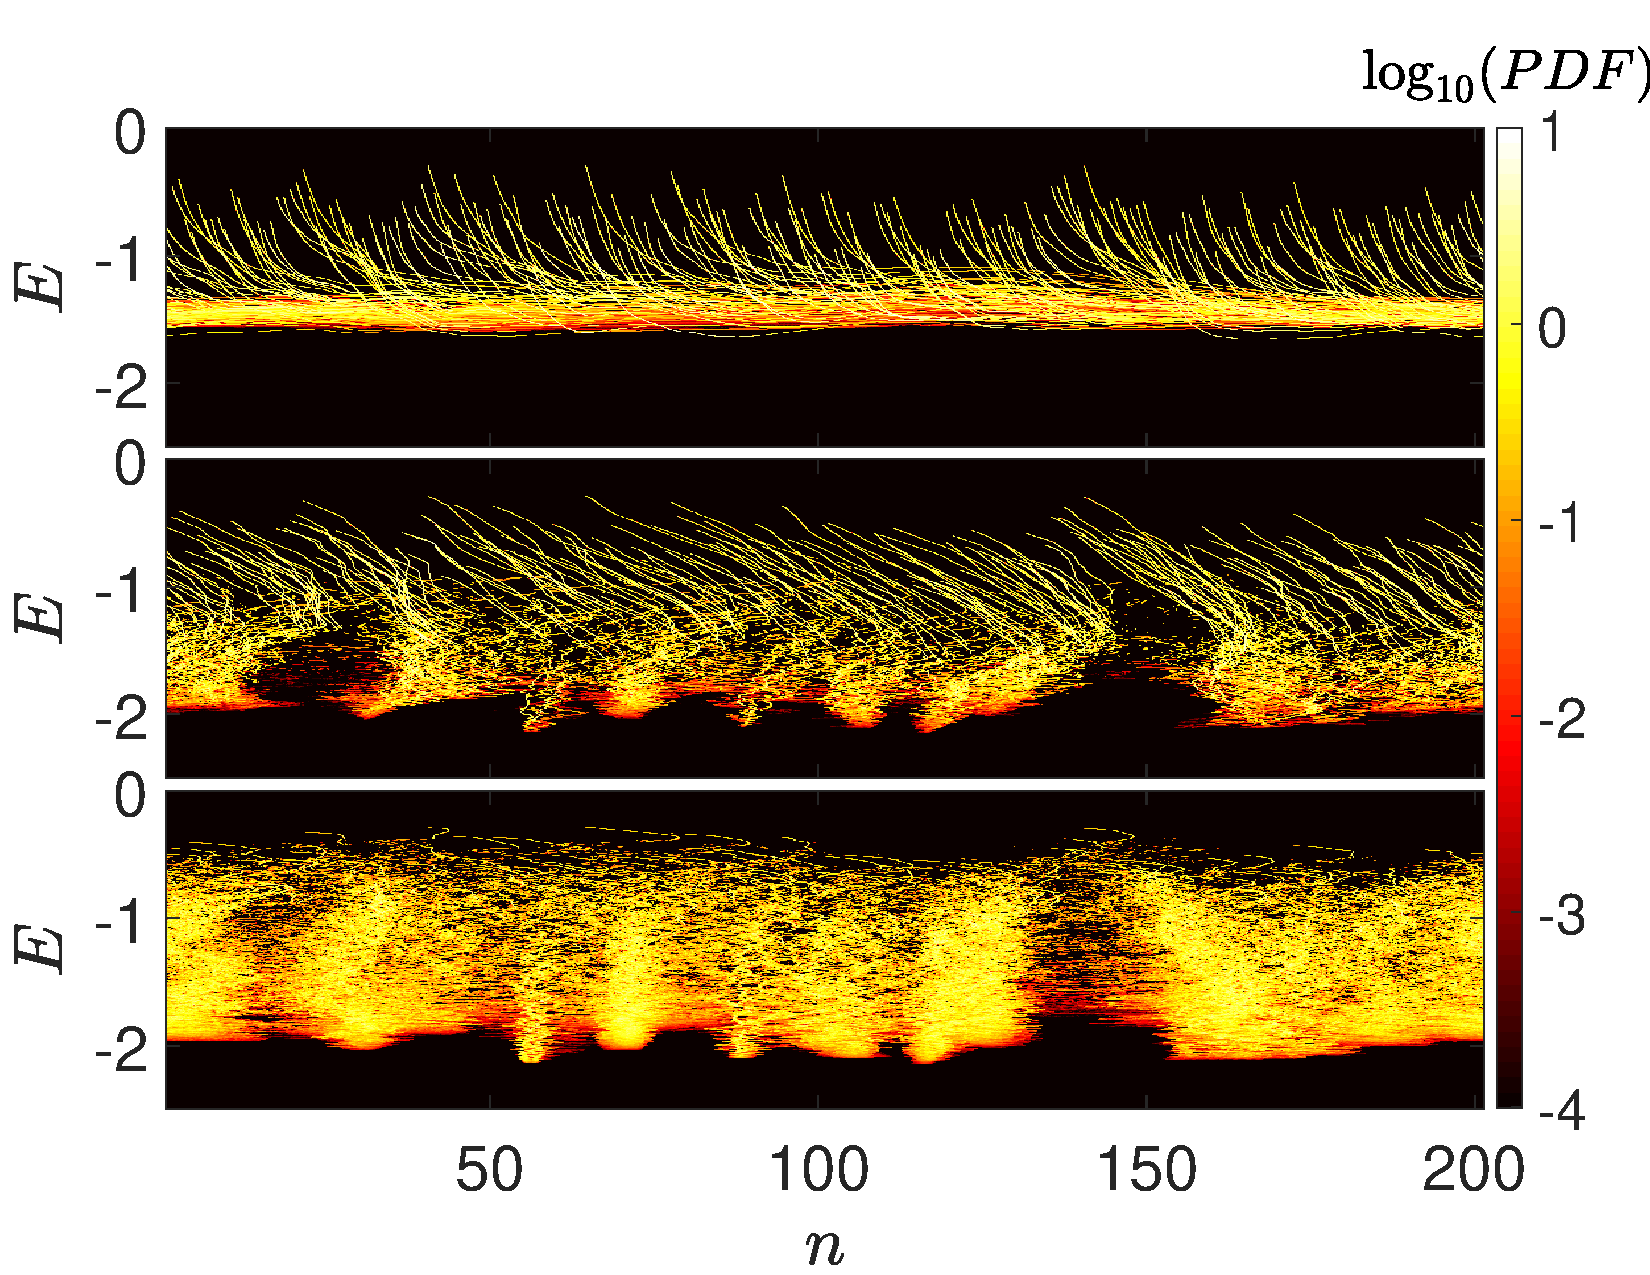
\includegraphics[width=0.5\linewidth]{anderson_prb_1_2}}
		\vfill
		\subcaptionbox[List-of-Figures entry]{\label{fig:anderson_prb_1_3}}{%
			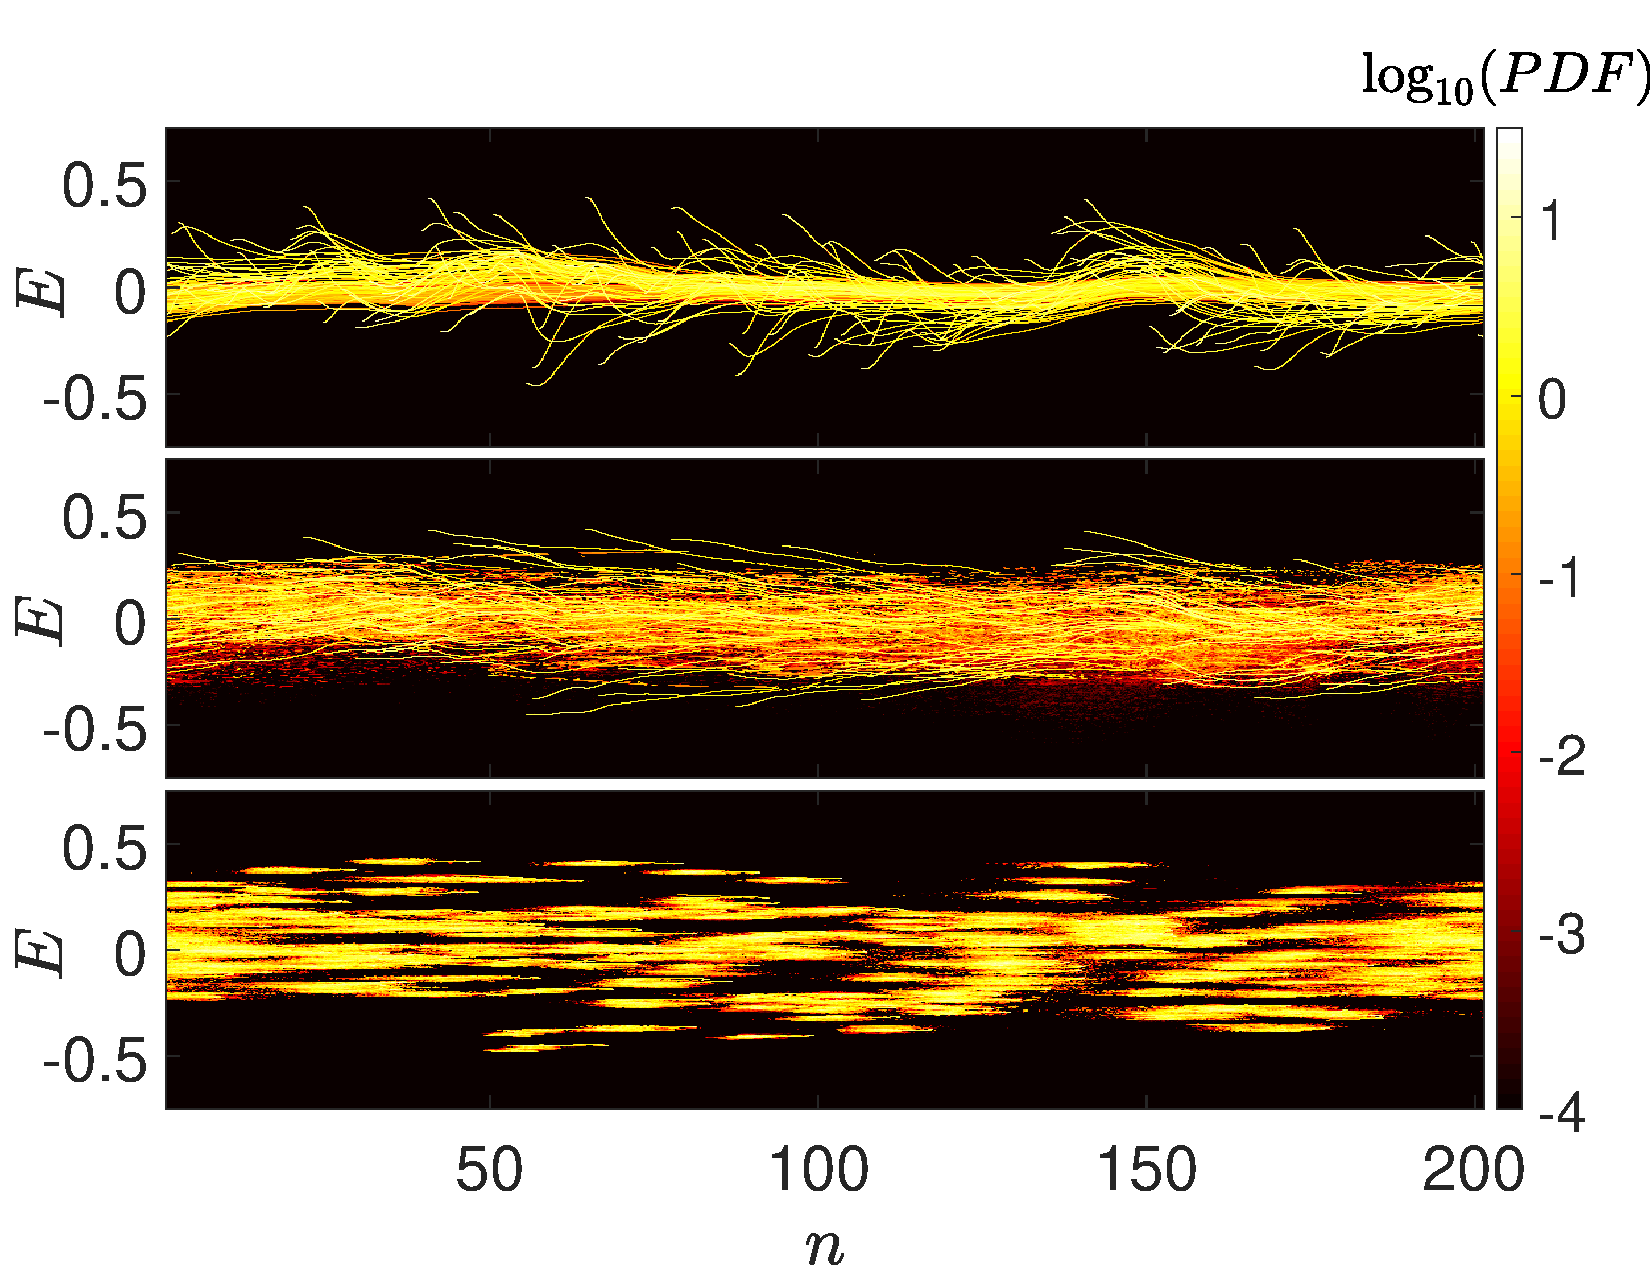
\includegraphics[width=0.5\linewidth]{anderson_prb_1_3}}
		\hfill
		\subcaptionbox{\label{fig:anderson_prb_1_4}}{%
			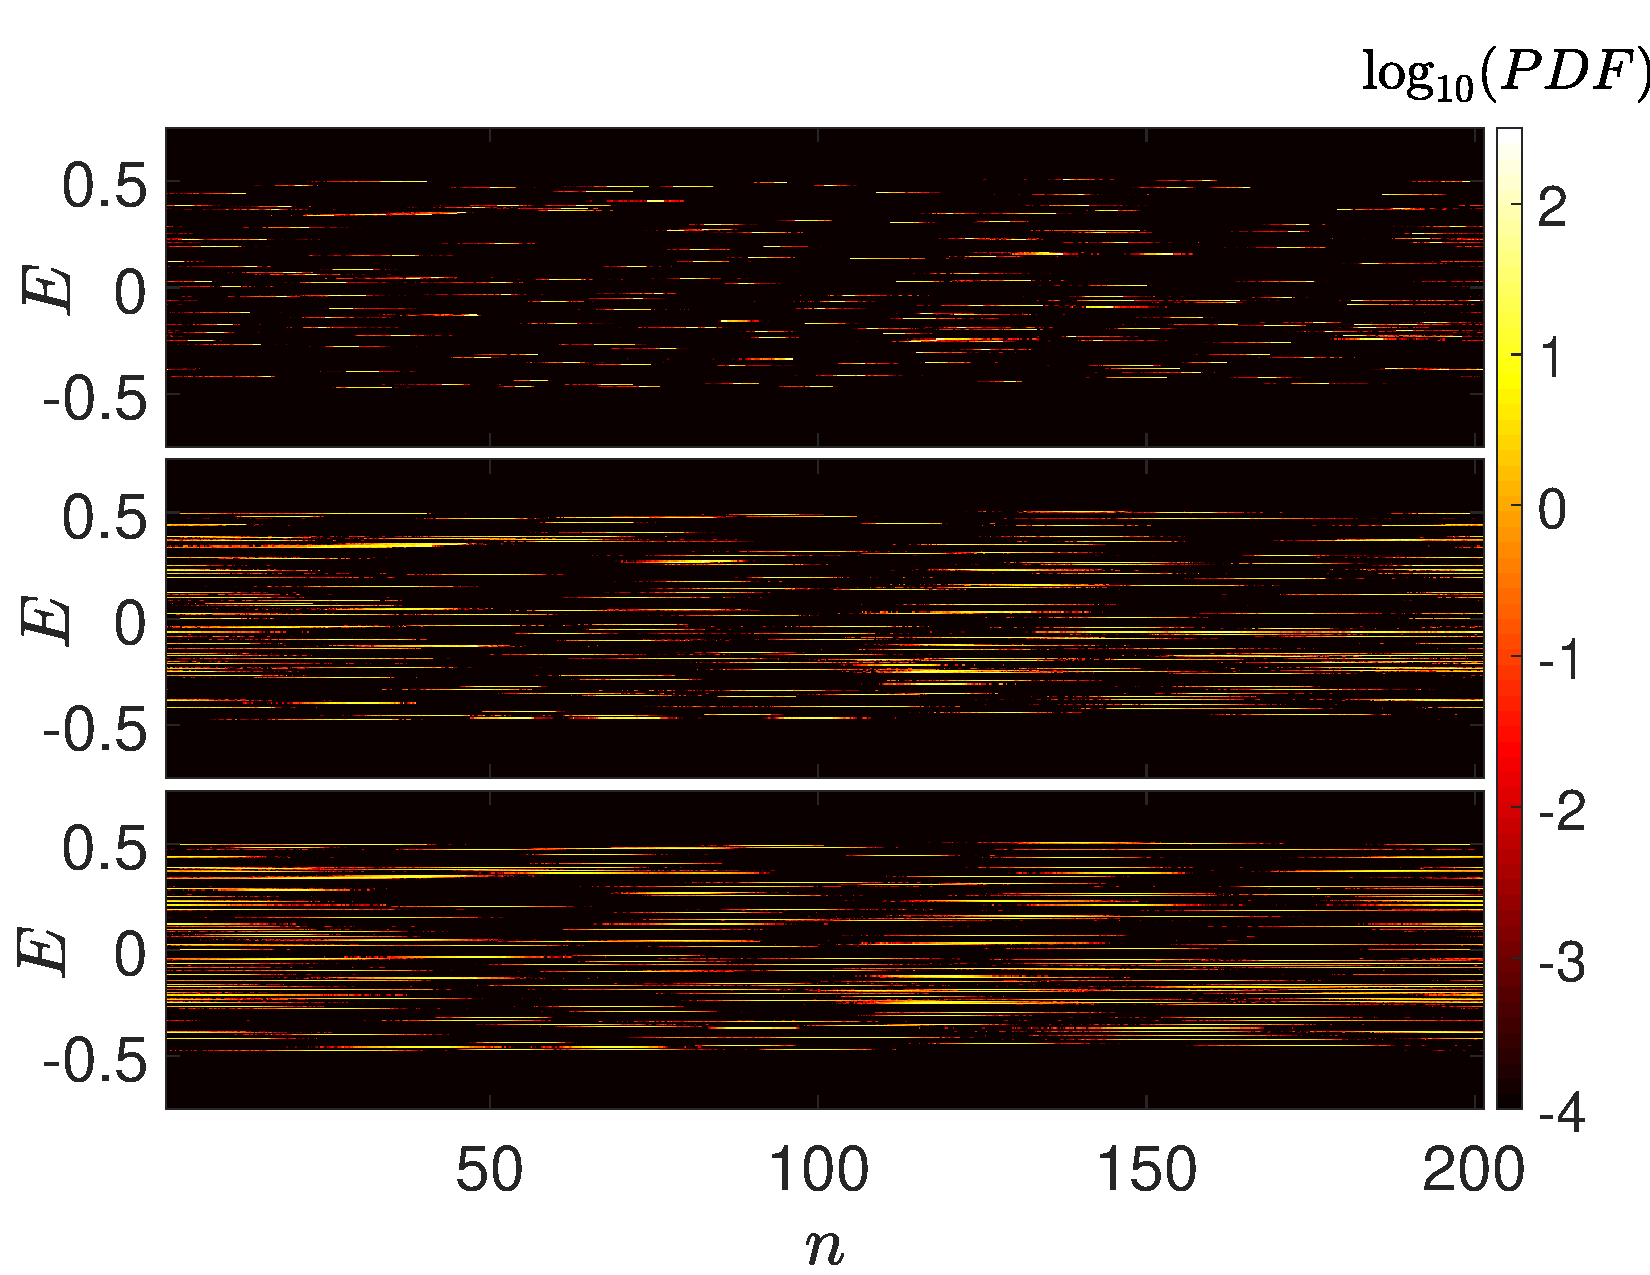
\includegraphics[width=0.5\linewidth]{anderson_prb_1_4}}
	}
	\legend{}
	\caption[Этот текст попадает в названия рисунков в списке рисунков]
	{
		Функция распределения плотности вероятностей (PDF) квантовых траекторий на плоскости позиции \(n(t)\) и энергии \(E(t))\) для \(\gamma=0.1\) (верхняя часть),  \(\gamma=0.01\) (центральная часть),  \(\gamma=0.001\) (нижняя часть). Результаты для локальных диссипаторов \cref{eq:anderson_diss_local} "--- (а): \(\alpha=0\); (б): \(\alpha=\frac{\pi}{4}\); (в): \(\alpha=\frac{\pi}{2}\). Дефазирующая диссипация "--- (г).
	}
	\label{fig:anderson_prb_1}
\end{figure}

Изучим структуру асимптотических состояний в виде двумерной функции плотности вероятностей нахождения траекторий на плоскости позиции \(n(t)\) \cref{eq:anderson_position} и энергии \(E(t)\) \cref{eq:anderson_energy} в зависимости от скорости диссипации \(\gamma\). На рисунке \cref{fig:anderson_prb_1} представлена типичная картина для фиксированной реализации беспорядка. При \(\alpha=0\) траектории стягиваются вокруг центров локализации, соединённых паутиной переходов, сходимость к центрам локализации и их компактность ослабевают с увеличением скорости диссипации (рисунок \cref{fig:anderson_prb_1_1}, сверху вниз).
Ненулевое значение фазы локальных диссипаторов \(\alpha=\frac{\pi}{4}\) приводит к сильному перекосу траекторий (рисунок \cref{fig:anderson_prb_1_2}). В конечном итоге, при \(\alpha=\frac{\pi}{2}\), центры локализации становятся плохо различимыми (рисунок \cref{fig:anderson_prb_1_3}). Следует отметить, что локализация энергии сохраняется, изменяясь от нижней границы спектра собственных чисел модели Андерсона \cref{eq:anderson_evals} при \(\alpha=0\) к середине спектра при \(\alpha=\frac{\pi}{2}\). Совсем иначе выглядит картина для случая дефазируюшей диссипации \cref{eq:anderson_diss_dephase}, при котором распределение плотности вероятности является случайным и охватывает весь спектр собственных значений модели Андерсона (рисунок \cref{fig:anderson_prb_1_4}).

\begin{figure}[ht]
	\centerfloat{
		\hfill
		\subcaptionbox[List-of-Figures entry]{\label{fig:anderson_prb_2_1}}{%
			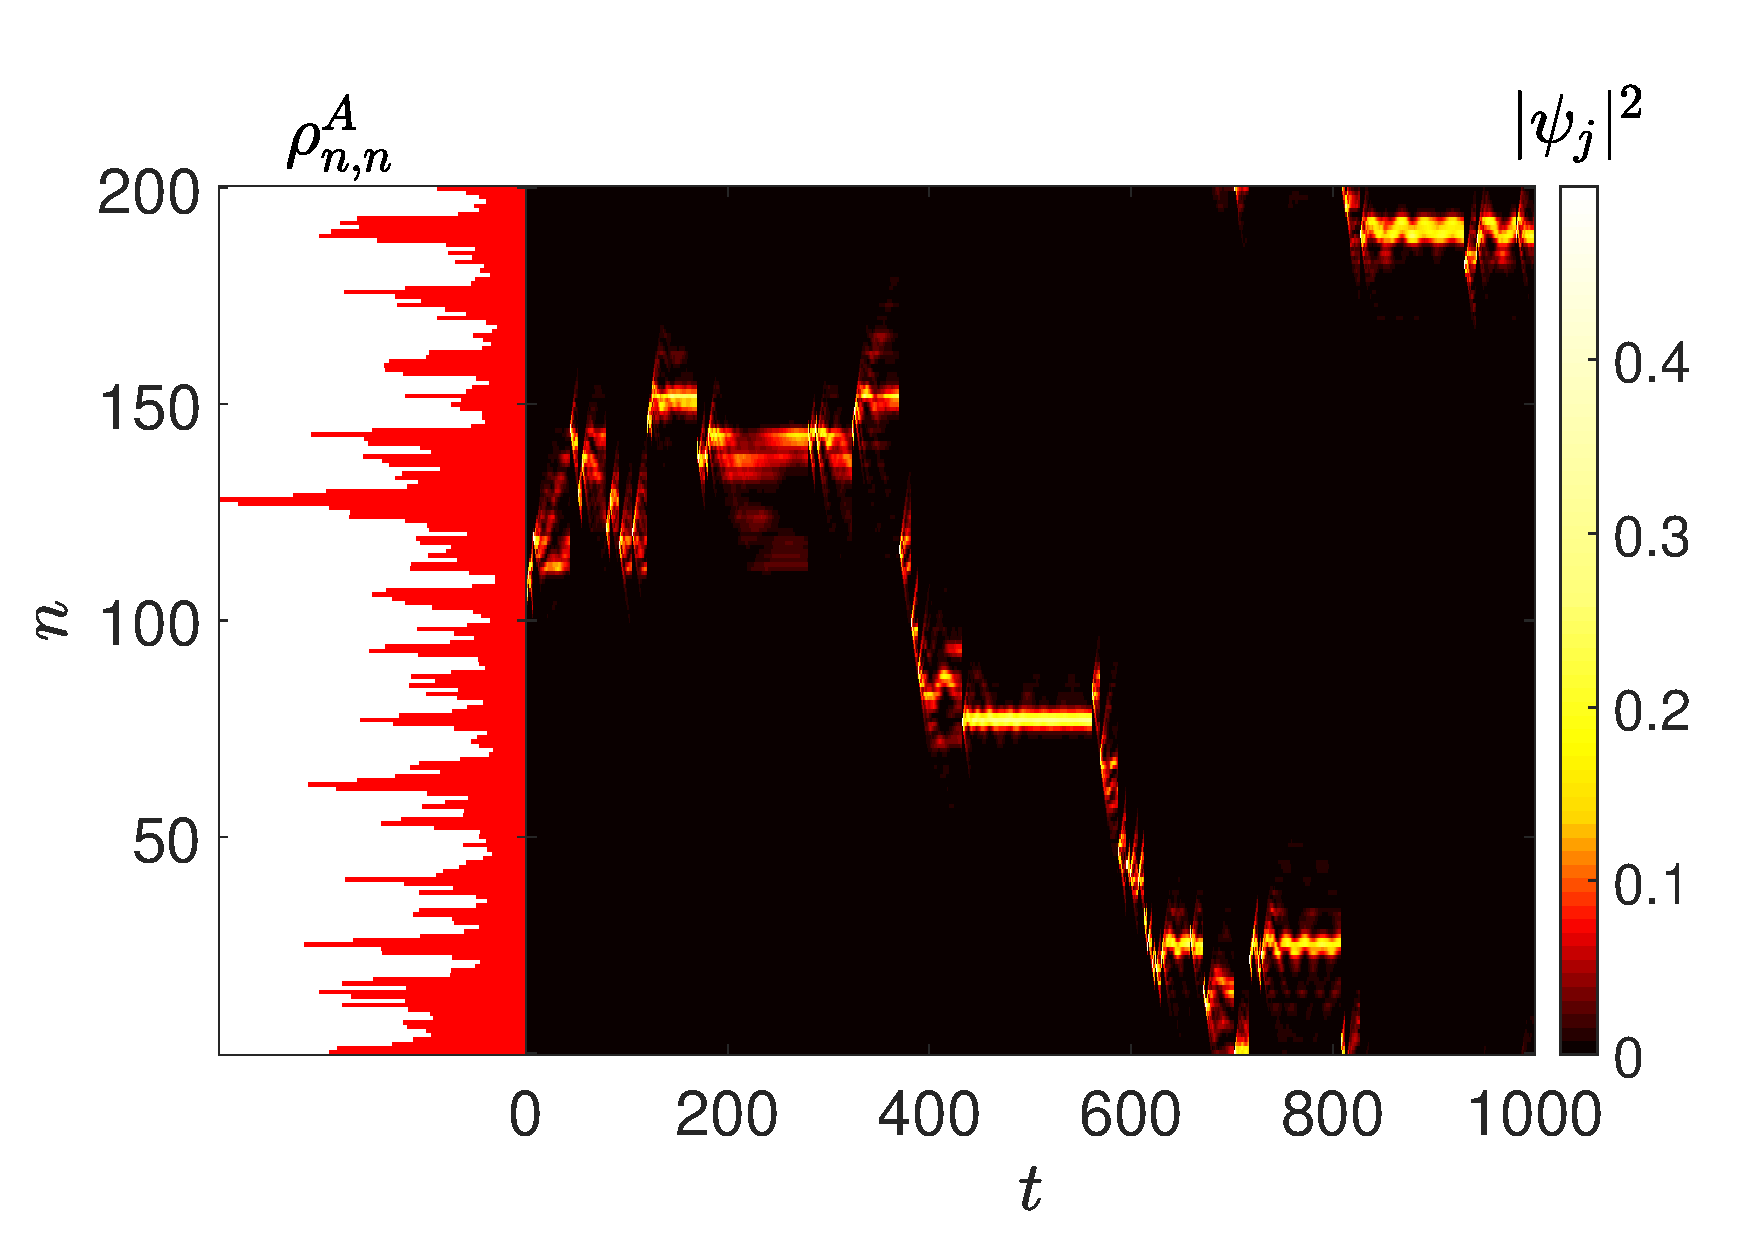
\includegraphics[width=0.5\linewidth]{anderson_prb_2_1}}
		\hfill
		\subcaptionbox{\label{fig:anderson_prb_2_2}}{%
			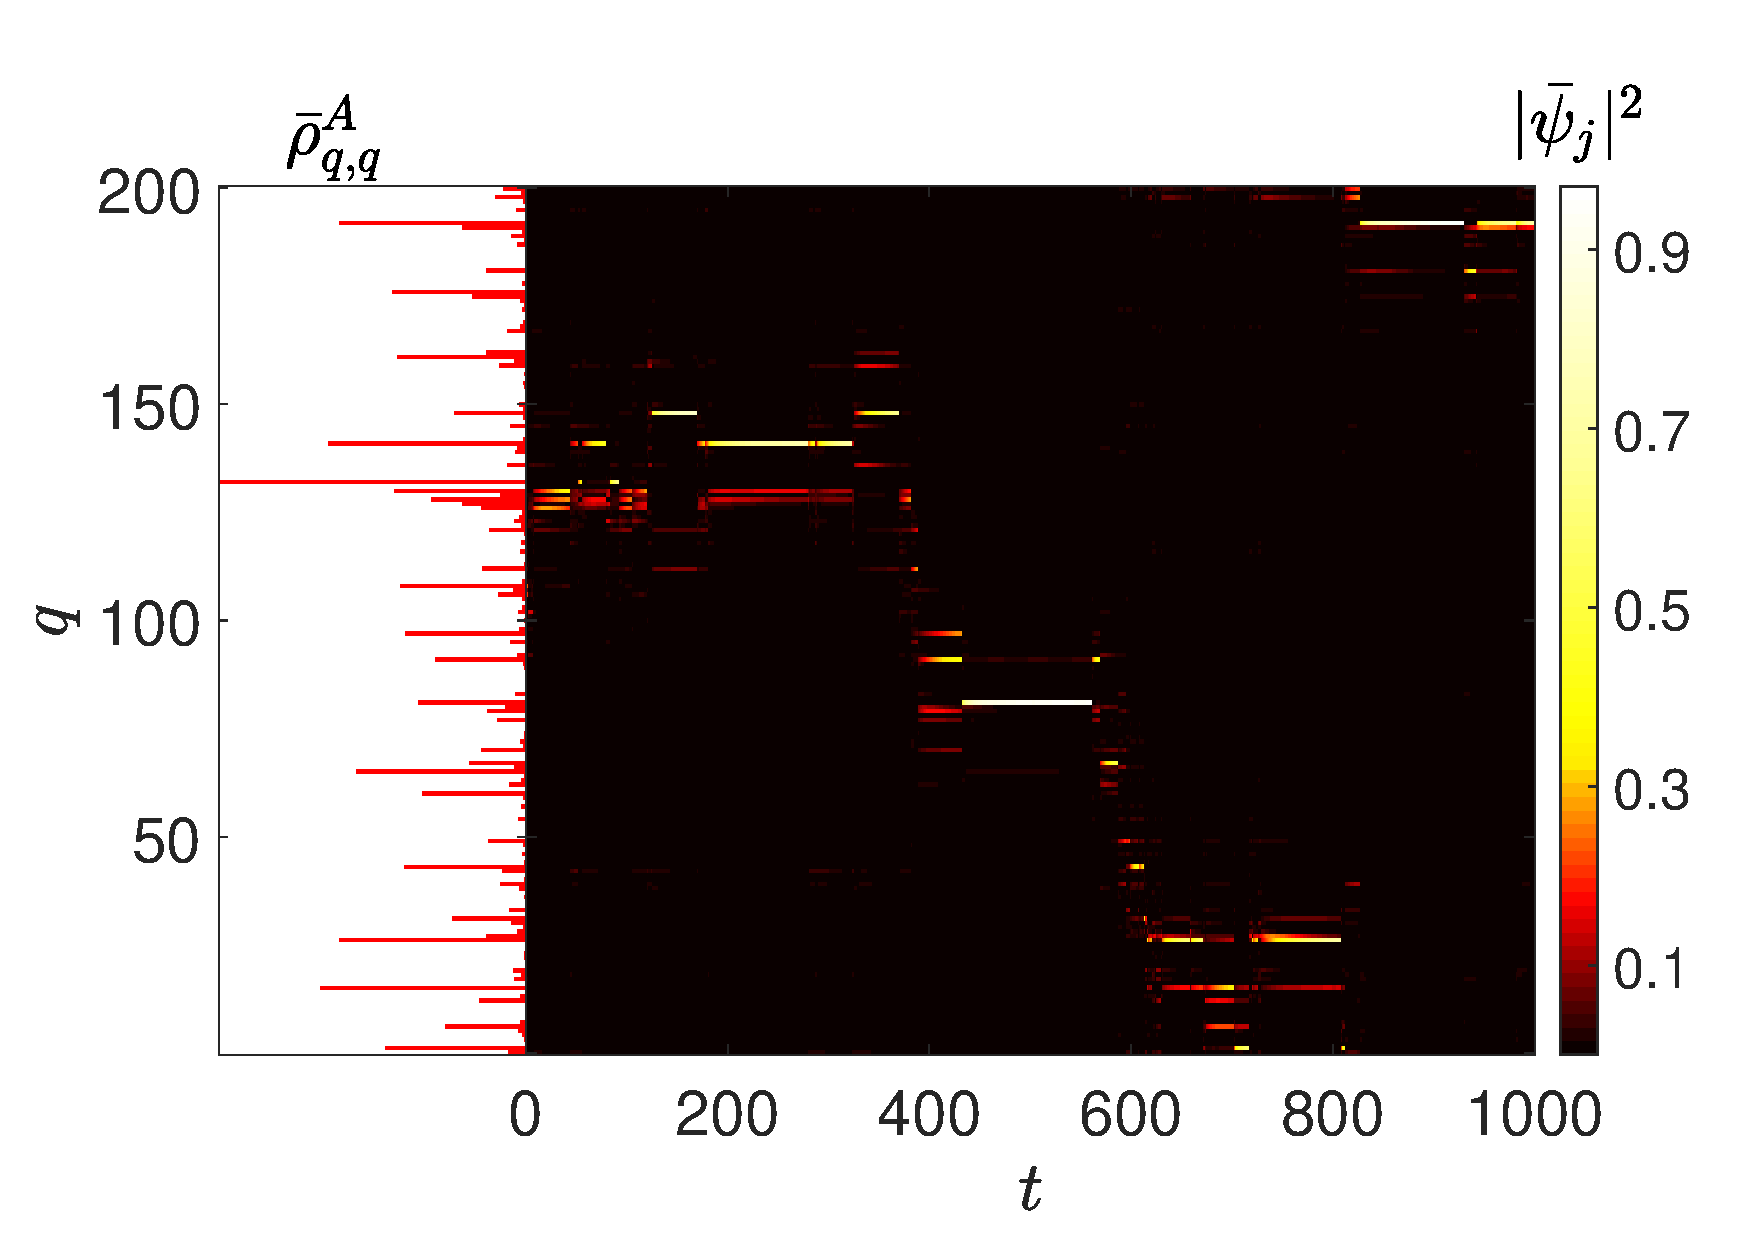
\includegraphics[width=0.5\linewidth]{anderson_prb_2_2}}
		\vfill
		\subcaptionbox[List-of-Figures entry]{\label{fig:anderson_prb_2_3}}{%
			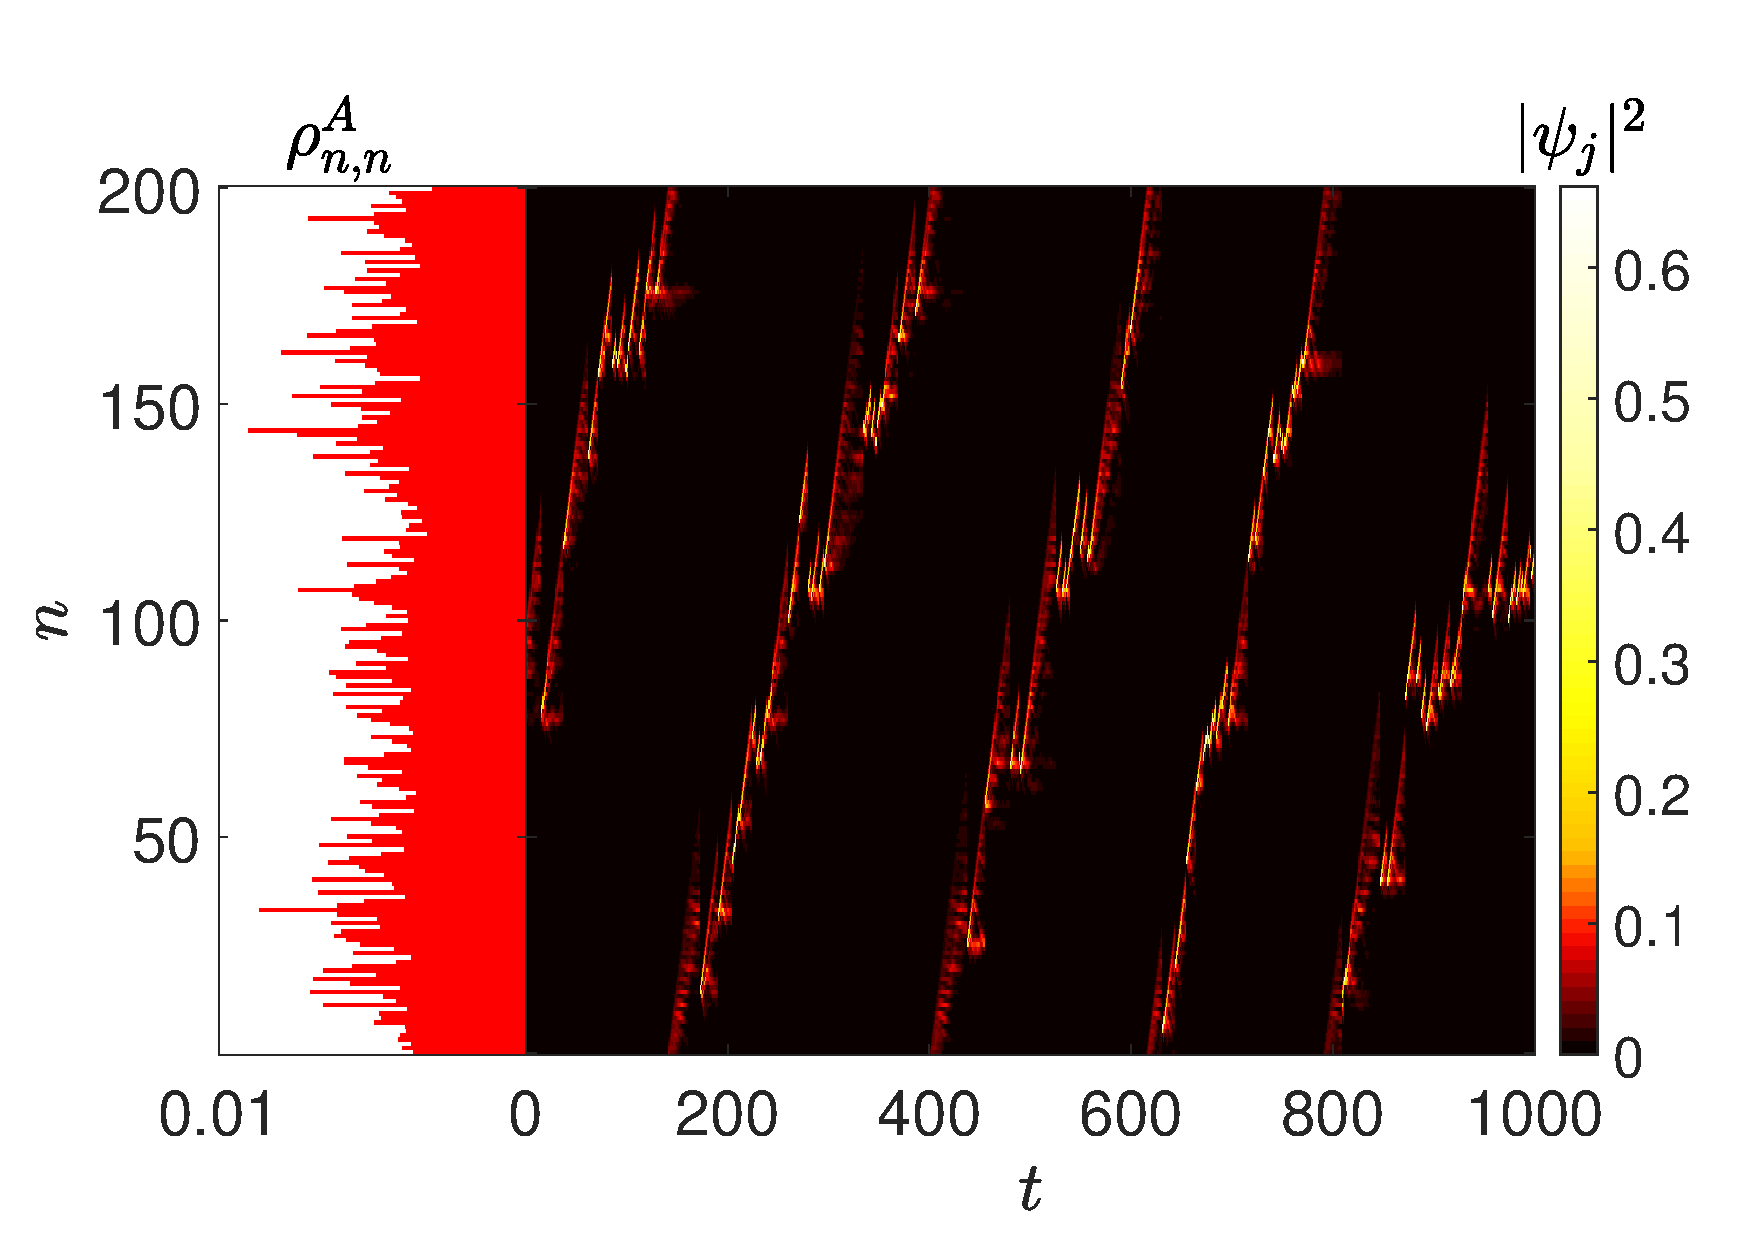
\includegraphics[width=0.5\linewidth]{anderson_prb_2_3}}
		\hfill
		\subcaptionbox{\label{fig:anderson_prb_2_4}}{%
			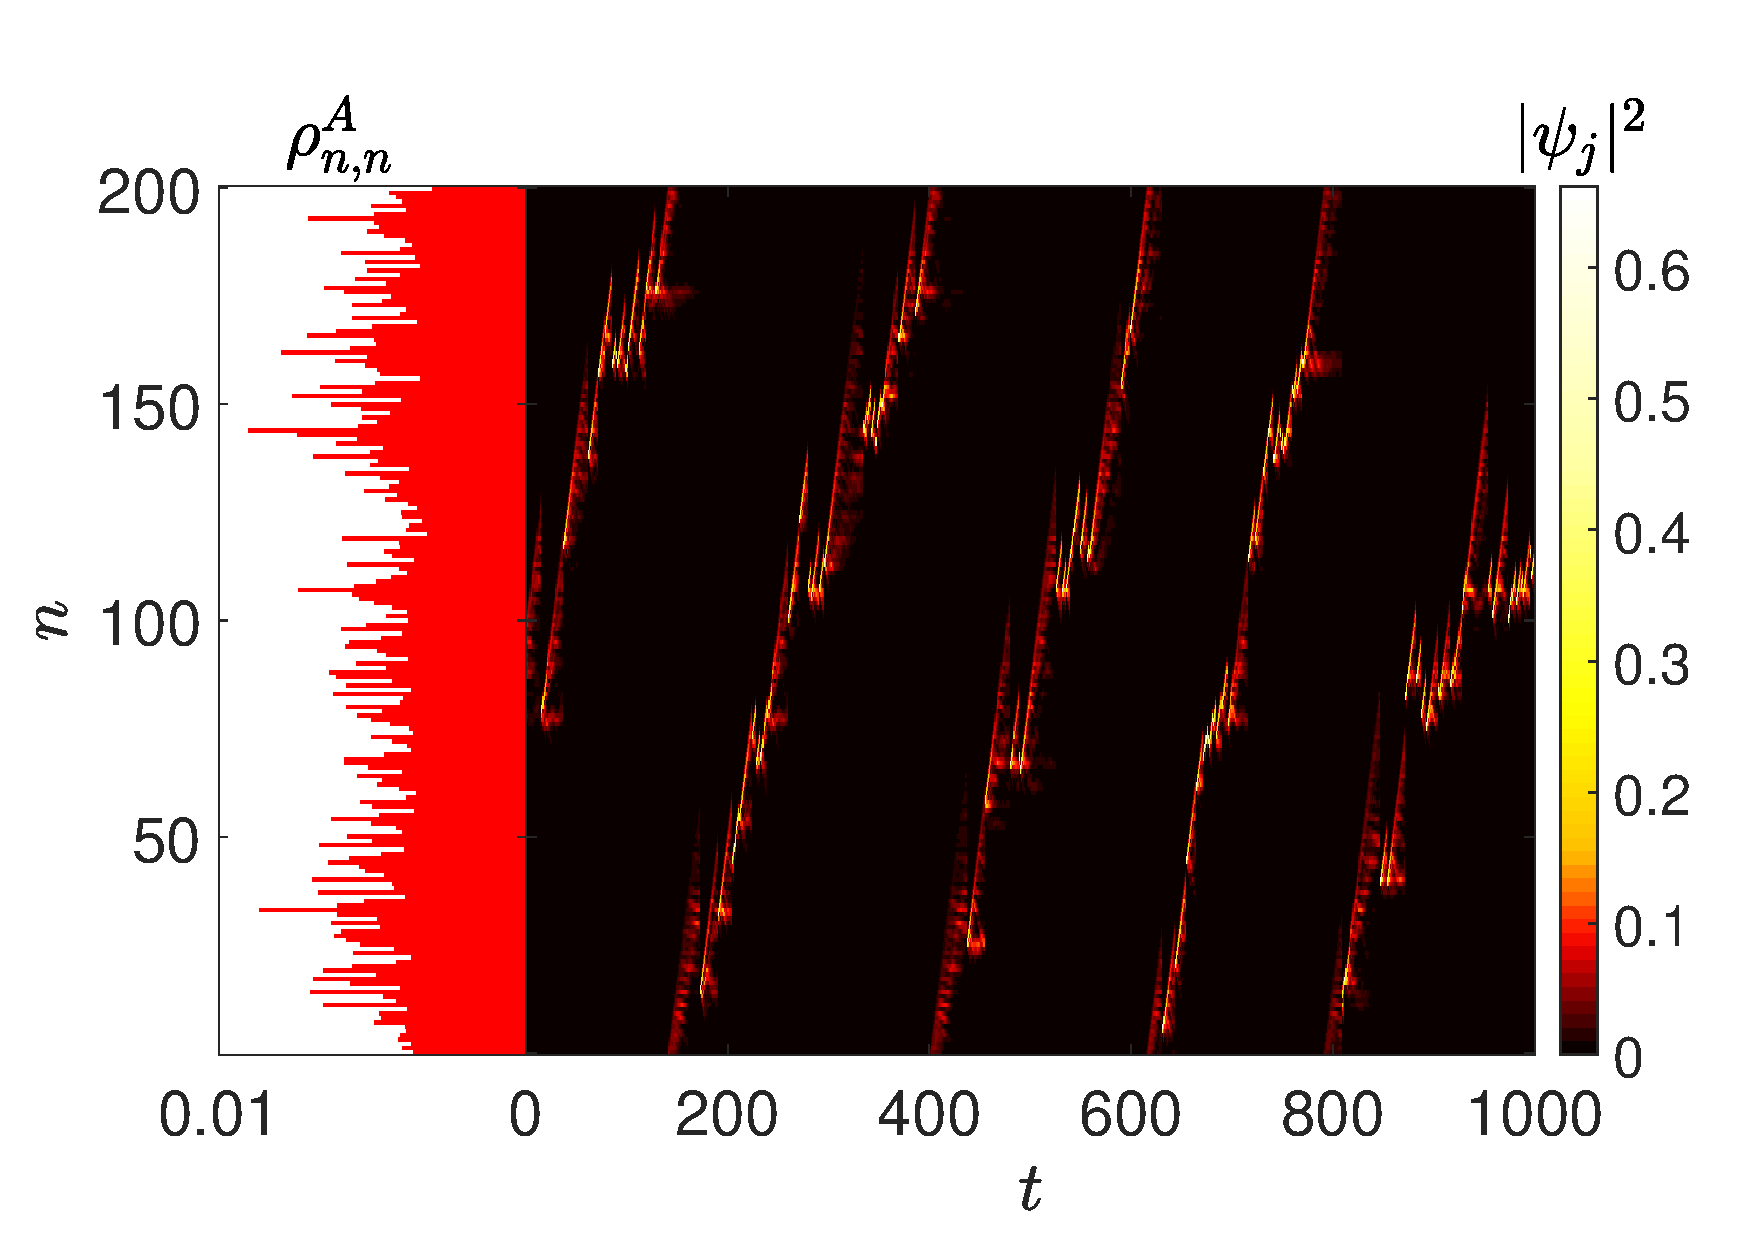
\includegraphics[width=0.5\linewidth]{anderson_prb_2_4}}
	}
	\legend{}
	\caption[Этот текст попадает в названия рисунков в списке рисунков]
	{
		aaa
	}
	\label{fig:anderson_prb_2}
\end{figure}

Исследуем теперь динамику волновых функций \(\psi_j(t)\) единичных квантовых траекторий (раздел \cref{sec:ch1/sec2}), которые эволюционируют с неэрмитовым гамитонианом \cref{eq:H_nonhermit}, в сопоставлении с асимптотическим состоянием \(\rho^A\) (или \(\bar{\rho}^A\) "--- в базисе собственных состояний модели Андерсона \cref{eq:anderson_rho_in_eigen_basis}). В случае нулевой фазы \(\alpha=0\) наблюдается прерывистая динамика состоящая из длительных циркуляций возле центров локализации и быстрых переходов между ними (рисунок \cref{fig:anderson_prb_2_1}).






Мы можем сделать \textbf{жирный текст} и \textit{курсив}.


Сошлёмся на библиографию.
Одна ссылка: \cite[с.~54]{Sokolov}\cite[с.~36]{Methodology}.
Две ссылки: \cite{Sokolov,Gaidaenko}.
Ссылка на собственные работы: \cite{Sokolov, Gaidaenko}.
Много ссылок: %\cite[с.~54]{Lermontov,Management,Borozda} % такой «фокус»
%вызывает biblatex warning относительно опции sortcites, потому что неясно, к
%какому источнику относится уточнение о страницах, а bibtex об этой проблеме
%даже не предупреждает
\cite{Lermontov, Management, Borozda, Marketing, Constitution, FamilyCode,
	Gost.7.0.53, Razumovski, Lagkueva, Pokrovski, Methodology, Berestova,
	Kriger}%
\ifnumequal{\value{bibliosel}}{0}{% Примеры для bibtex8
	\cite{Sirotko, Lukina, Encyclopedia, Nasirova}%
}{% Примеры для biblatex через движок biber
	\cite{Sirotko2, Lukina2, Encyclopedia2, Nasirova2}%
}%
.
И~ещё немного ссылок:~\cite{Article,Book,Booklet,Conference,Inbook,Incollection,Manual,Mastersthesis,
	Misc,Phdthesis,Proceedings,Techreport,Unpublished}
% Следует обратить внимание, что пробел после запятой внутри \cite{}
% обрабатывается ожидаемо, а пробел перед запятой, может вызывать проблемы при
% обработке ссылок.
\cite{medvedev2006jelektronnye, CEAT:CEAT581, doi:10.1080/01932691.2010.513279,
	Gosele1999161,Li2007StressAnalysis, Shoji199895, test:eisner-sample,
	test:eisner-sample-shorted, AB_patent_Pomerantz_1968, iofis_patent1960}
\ifnumequal{\value{bibliosel}}{0}{% Примеры для bibtex8
}{% Примеры для biblatex через движок biber
	\cite{patent2h, patent3h, patent2}%
}%
.

\ifnumequal{\value{bibliosel}}{0}{% Примеры для bibtex8
	Попытка реализовать несколько ссылок на конкретные страницы
	для \texttt{bibtex} реализации библиографии:
	[\citenum{Sokolov}, с.~54; \citenum{Gaidaenko}, с.~36].
}{% Примеры для biblatex через движок biber
	Несколько источников (мультицитата):
	% Тут специально написано по-разному тире, для демонстрации, что
	% применение специальных тире в настоящий момент в biblatex приводит к непоказу
	% "с.".
	\cites[vii--x, 5, 7]{Sokolov}[v"--~x, 25, 526]{Gaidaenko}[vii--x, 5, 7]{Techreport},
	работает только в \texttt{biblatex} реализации библиографии.
}%

Ссылки на собственные работы:~\cite{Sokolov, Gaidaenko}

Сошлёмся на приложения: Приложение~\cref{app:A}, Приложение~\cref{app:B2}.

Сошлёмся на формулу: формула~\cref{eq:equation1}.

Сошлёмся на изображение: рисунок~\cref{fig:knuth}.

Стандартной практикой является добавление к ссылкам префикса, характеризующего тип элемента.
Это не является строгим требованием, но~позволяет лучше ориентироваться в документах большого размера.
Например, для ссылок на~рисунки используется префикс \textit{fig},
для ссылки на~таблицу "--- \textit{tab}.

В таблице \cref{tab:tab_pref} приложения~\cref{app:B4} приведён список рекомендуемых
к использованию стандартных префиксов.

Благодаря пакету \textit{icomma}, \LaTeX~одинаково хорошо воспринимает
в~качестве десятичного разделителя и запятую (\(3,1415\)), и точку (\(3.1415\)).

\subsection{Ненумерованные одиночные формулы}\label{subsec:ch1/sec3/sub1}

Вот так может выглядеть формула, которую необходимо вставить в~строку
по~тексту: \(x \approx \sin x\) при \(x \to 0\).

А вот так выглядит ненумерованная отдельностоящая формула c подстрочными
и надстрочными индексами:
\[
(x_1+x_2)^2 = x_1^2 + 2 x_1 x_2 + x_2^2
\]

Формула с неопределенным интегралом:
\[
\int f(\alpha+x)=\sum\beta
\]

При использовании дробей формулы могут получаться очень высокие:
\[
  \frac{1}{\sqrt{2}+
  \displaystyle\frac{1}{\sqrt{2}+
  \displaystyle\frac{1}{\sqrt{2}+\cdots}}}
\]

В формулах можно использовать греческие буквы:
%Все \original... команды заранее, ради этого примера, определены в Dissertation\userstyles.tex
\[
\alpha\beta\gamma\delta\originalepsilon\epsilon\zeta\eta\theta%
\vartheta\iota\kappa\varkappa\lambda\mu\nu\xi\pi\varpi\rho\varrho%
\sigma\varsigma\tau\upsilon\originalphi\phi\chi\psi\omega\Gamma\Delta%
\Theta\Lambda\Xi\Pi\Sigma\Upsilon\Phi\Psi\Omega
\]
\[%https://texfaq.org/FAQ-boldgreek
\boldsymbol{\alpha\beta\gamma\delta\originalepsilon\epsilon\zeta\eta%
\theta\vartheta\iota\kappa\varkappa\lambda\mu\nu\xi\pi\varpi\rho%
\varrho\sigma\varsigma\tau\upsilon\originalphi\phi\chi\psi\omega\Gamma%
\Delta\Theta\Lambda\Xi\Pi\Sigma\Upsilon\Phi\Psi\Omega}
\]

Для добавления формул можно использовать пары \verb+$+\dots\verb+$+ и \verb+$$+\dots\verb+$$+,
но~они считаются устаревшими.
Лучше использовать их функциональные аналоги \verb+\(+\dots\verb+\)+ и \verb+\[+\dots\verb+\]+.

\subsection{Ненумерованные многострочные формулы}\label{subsec:ch1/sec3/sub2}

Вот так можно написать две формулы, не нумеруя их, чтобы знаки <<равно>> были
строго друг под другом:
\begin{align}
  f_W & =  \min \left( 1, \max \left( 0, \frac{W_{soil} / W_{max}}{W_{crit}} \right)  \right), \nonumber \\
  f_T & =  \min \left( 1, \max \left( 0, \frac{T_s / T_{melt}}{T_{crit}} \right)  \right), \nonumber
\end{align}

Выровнять систему ещё и по переменной \( x \) можно, используя окружение
\verb|alignedat| из пакета \verb|amsmath|. Вот так:
\[
    |x| = \left\{
    \begin{alignedat}{2}
        &&x, \quad &\text{eсли } x\geqslant 0 \\
        &-&x, \quad & \text{eсли } x<0
    \end{alignedat}
    \right.
\]
Здесь первый амперсанд (в исходном \LaTeX\ описании формулы) означает
выравнивание по~левому краю, второй "--- по~\( x \), а~третий "--- по~слову
<<если>>. Команда \verb|\quad| делает большой горизонтальный пробел.

Ещё вариант:
\[
    |x|=
    \begin{cases}
    \phantom{-}x, \text{если } x \geqslant 0 \\
    -x, \text{если } x<0
    \end{cases}
\]

Кроме того, для  нумерованных формул \verb|alignedat| делает вертикальное
выравнивание номера формулы по центру формулы. Например, выравнивание
компонент вектора:
\begin{equation}
\label{eq:2p3}
\begin{alignedat}{2}
{\mathbf{N}}_{o1n}^{(j)} = \,{\sin} \phi\,n\!\left(n+1\right)
         {\sin}\theta\,
         \pi_n\!\left({\cos} \theta\right)
         \frac{
               z_n^{(j)}\!\left( \rho \right)
              }{\rho}\,
           &{\boldsymbol{\hat{\mathrm e}}}_{r}\,+   \\
+\,
{\sin} \phi\,
         \tau_n\!\left({\cos} \theta\right)
         \frac{
            \left[\rho z_n^{(j)}\!\left( \rho \right)\right]^{\prime}
              }{\rho}\,
            &{\boldsymbol{\hat{\mathrm e}}}_{\theta}\,+   \\
+\,
{\cos} \phi\,
         \pi_n\!\left({\cos} \theta\right)
         \frac{
            \left[\rho z_n^{(j)}\!\left( \rho \right)\right]^{\prime}
              }{\rho}\,
            &{\boldsymbol{\hat{\mathrm e}}}_{\phi}\:.
\end{alignedat}
\end{equation}

Ещё об отступах. Иногда для лучшей <<читаемости>> формул полезно
немного исправить стандартные интервалы \LaTeX\ с учётом логической
структуры самой формулы. Например в формуле~\cref{eq:2p3} добавлен
небольшой отступ \verb+\,+ между основными сомножителями, ниже
результат применения всех вариантов отступа:
\begin{align*}
\backslash! &\quad f(x) = x^2\! +3x\! +2 \\
  \mbox{по-умолчанию} &\quad f(x) = x^2+3x+2 \\
\backslash, &\quad f(x) = x^2\, +3x\, +2 \\
\backslash{:} &\quad f(x) = x^2\: +3x\: +2 \\
\backslash; &\quad f(x) = x^2\; +3x\; +2 \\
\backslash \mbox{space} &\quad f(x) = x^2\ +3x\ +2 \\
\backslash \mbox{quad} &\quad f(x) = x^2\quad +3x\quad +2 \\
\backslash \mbox{qquad} &\quad f(x) = x^2\qquad +3x\qquad +2
\end{align*}

Можно использовать разные математические алфавиты:
\begin{align}
\mathcal{ABCDEFGHIJKLMNOPQRSTUVWXYZ} \nonumber \\
\mathfrak{ABCDEFGHIJKLMNOPQRSTUVWXYZ} \nonumber \\
\mathbb{ABCDEFGHIJKLMNOPQRSTUVWXYZ} \nonumber
\end{align}

Посмотрим на систему уравнений на примере аттрактора Лоренца:

\[
\left\{
  \begin{array}{rl}
    \dot x = & \sigma (y-x) \\
    \dot y = & x (r - z) - y \\
    \dot z = & xy - bz
  \end{array}
\right.
\]

А для вёрстки матриц удобно использовать многоточия:
\[
\left(
  \begin{array}{ccc}
    a_{11} & \ldots & a_{1n} \\
    \vdots & \ddots & \vdots \\
    a_{n1} & \ldots & a_{nn} \\
  \end{array}
\right)
\]

\subsection{Нумерованные формулы}\label{subsec:ch1/sec3/sub3}

А вот так пишется нумерованная формула:
\begin{equation}
  \label{eq:equation1}
  e = \lim_{n \to \infty} \left( 1+\frac{1}{n} \right) ^n
\end{equation}

Нумерованных формул может быть несколько:
\begin{equation}
  \label{eq:equation2}
  \lim_{n \to \infty} \sum_{k=1}^n \frac{1}{k^2} = \frac{\pi^2}{6}
\end{equation}

Впоследствии на формулы~\cref{eq:equation1, eq:equation2} можно ссылаться.

Сделать так, чтобы номер формулы стоял напротив средней строки, можно,
используя окружение \verb|multlined| (пакет \verb|mathtools|) вместо
\verb|multline| внутри окружения \verb|equation|. Вот так:
\begin{equation} % \tag{S} % tag - вписывает свой текст
  \label{eq:equation3}
    \begin{multlined}
        1+ 2+3+4+5+6+7+\dots + \\
        + 50+51+52+53+54+55+56+57 + \dots + \\
        + 96+97+98+99+100=5050
    \end{multlined}
\end{equation}

Уравнения~\cref{eq:subeq_1,eq:subeq_2} демонстрируют возможности
окружения \verb|\subequations|.
\begin{subequations}
    \label{eq:subeq_1}
    \begin{gather}
        y = x^2 + 1 \label{eq:subeq_1-1} \\
        y = 2 x^2 - x + 1 \label{eq:subeq_1-2}
    \end{gather}
\end{subequations}
Ссылки на отдельные уравнения~\cref{eq:subeq_1-1,eq:subeq_1-2,eq:subeq_2-1}.
\begin{subequations}
    \label{eq:subeq_2}
    \begin{align}
        y &= x^3 + x^2 + x + 1 \label{eq:subeq_2-1} \\
        y &= x^2
    \end{align}
\end{subequations}

\subsection{Форматирование чисел и размерностей величин}\label{sec:units}

Числа форматируются при помощи команды \verb|\num|:
\num{5,3};
\num{2,3e8};
\num{12345,67890};
\num{2,6 d4};
\num{1+-2i};
\num{.3e45};
\num[exponent-base=2]{5 e64};
\num[exponent-base=2,exponent-to-prefix]{5 e64};
\num{1.654 x 2.34 x 3.430}
\num{1 2 x 3 / 4}.
Для написания последовательности чисел можно использовать команды \verb|\numlist| и \verb|\numrange|:
\numlist{10;30;50;70}; \numrange{10}{30}.
Значения углов можно форматировать при помощи команды \verb|\ang|:
\ang{2.67};
\ang{30,3};
\ang{-1;;};
\ang{;-2;};
\ang{;;-3};
\ang{300;10;1}.

Обратите внимание, что ГОСТ запрещает использование знака <<->> для обозначения отрицательных чисел
за исключением формул, таблиц и~рисунков.
Вместо него следует использовать слово <<минус>>.

Размерности можно записывать при помощи команд \verb|\si| и \verb|\SI|:
\si{\farad\squared\lumen\candela};
\si{\joule\per\mole\per\kelvin};
\si[per-mode = symbol-or-fraction]{\joule\per\mole\per\kelvin};
\si{\metre\per\second\squared};
\SI{0.10(5)}{\neper};
\SI{1.2-3i e5}{\joule\per\mole\per\kelvin};
\SIlist{1;2;3;4}{\tesla};
\SIrange{50}{100}{\volt}.
Список единиц измерений приведён в таблицах~\cref{tab:unit:base,
tab:unit:derived,tab:unit:accepted,tab:unit:physical,tab:unit:other}.
Приставки единиц приведены в~таблице~\cref{tab:unit:prefix}.

С дополнительными опциями форматирования можно ознакомиться в~описании пакета \texttt{siunitx};
изменить или добавить единицы измерений можно в~файле \texttt{siunitx.cfg}.

\begin{table}
    \centering
    \captionsetup{justification=centering} % выравнивание подписи по-центру
    \caption{Основные величины СИ}\label{tab:unit:base}
    \begin{tabular}{llc}
        \toprule
        Название  & Команда                & Символ         \\
        \midrule
        Ампер     & \verb|\ampere| & \si{\ampere}   \\
        Кандела   & \verb|\candela| & \si{\candela}  \\
        Кельвин   & \verb|\kelvin| & \si{\kelvin}   \\
        Килограмм & \verb|\kilogram| & \si{\kilogram} \\
        Метр      & \verb|\metre| & \si{\metre}    \\
        Моль      & \verb|\mole| & \si{\mole}     \\
        Секунда   & \verb|\second| & \si{\second}   \\
        \bottomrule
    \end{tabular}
\end{table}

\begin{table}
  \small
  \centering
  \begin{threeparttable}% выравнивание подписи по границам таблицы
    \caption{Производные единицы СИ}\label{tab:unit:derived}
    \begin{tabular}{llc|llc}
        \toprule
        Название       & Команда                 & Символ              & Название & Команда & Символ \\
        \midrule
        Беккерель      & \verb|\becquerel|  & \si{\becquerel}     &
        Ньютон         & \verb|\newton|  & \si{\newton}                                      \\
        Градус Цельсия & \verb|\degreeCelsius| & \si{\degreeCelsius} &
        Ом             & \verb|\ohm| & \si{\ohm}                                         \\
        Кулон          & \verb|\coulomb| & \si{\coulomb}       &
        Паскаль        & \verb|\pascal| & \si{\pascal}                                      \\
        Фарад          & \verb|\farad| & \si{\farad}         &
        Радиан         & \verb|\radian| & \si{\radian}                                      \\
        Грей           & \verb|\gray| & \si{\gray}          &
        Сименс         & \verb|\siemens| & \si{\siemens}                                     \\
        Герц           & \verb|\hertz| & \si{\hertz}         &
        Зиверт         & \verb|\sievert| & \si{\sievert}                                     \\
        Генри          & \verb|\henry| & \si{\henry}         &
        Стерадиан      & \verb|\steradian| & \si{\steradian}                                   \\
        Джоуль         & \verb|\joule| & \si{\joule}         &
        Тесла          & \verb|\tesla| & \si{\tesla}                                       \\
        Катал          & \verb|\katal| & \si{\katal}         &
        Вольт          & \verb|\volt| & \si{\volt}                                        \\
        Люмен          & \verb|\lumen| & \si{\lumen}         &
        Ватт           & \verb|\watt| & \si{\watt}                                        \\
        Люкс           & \verb|\lux| & \si{\lux}           &
        Вебер          & \verb|\weber| & \si{\weber}                                       \\
        \bottomrule
    \end{tabular}
  \end{threeparttable}
\end{table}

\begin{table}
  \centering
  \begin{threeparttable}% выравнивание подписи по границам таблицы
    \caption{Внесистемные единицы}\label{tab:unit:accepted}

    \begin{tabular}{llc}
        \toprule
        Название        & Команда                 & Символ          \\
        \midrule
        День            & \verb|\day| & \si{\day}       \\
        Градус          & \verb|\degree| & \si{\degree}    \\
        Гектар          & \verb|\hectare| & \si{\hectare}   \\
        Час             & \verb|\hour| & \si{\hour}      \\
        Литр            & \verb|\litre| & \si{\litre}     \\
        Угловая минута  & \verb|\arcminute| & \si{\arcminute} \\
        Угловая секунда & \verb|\arcsecond| & \si{\arcsecond} \\ %
        Минута          & \verb|\minute| & \si{\minute}    \\
        Тонна           & \verb|\tonne| & \si{\tonne}     \\
        \bottomrule
    \end{tabular}
  \end{threeparttable}
\end{table}

\begin{table}
    \centering
    \captionsetup{justification=centering}
    \caption{Внесистемные единицы, получаемые из эксперимента}\label{tab:unit:physical}
    \begin{tabular}{llc}
        \toprule
        Название                & Команда                 & Символ                 \\
        \midrule
        Астрономическая единица & \verb|\astronomicalunit| & \si{\astronomicalunit} \\
        Атомная единица массы   & \verb|\atomicmassunit| & \si{\atomicmassunit}   \\
        Боровский радиус        & \verb|\bohr| & \si{\bohr}             \\
        Скорость света          & \verb|\clight| & \si{\clight}           \\
        Дальтон                 & \verb|\dalton| & \si{\dalton}           \\
        Масса электрона         & \verb|\electronmass| & \si{\electronmass}     \\
        Электрон Вольт          & \verb|\electronvolt| & \si{\electronvolt}     \\
        Элементарный заряд      & \verb|\elementarycharge| & \si{\elementarycharge} \\
        Энергия Хартри          & \verb|\hartree| & \si{\hartree}          \\
        Постоянная Планка       & \verb|\planckbar| & \si{\planckbar}        \\
        \bottomrule
    \end{tabular}
\end{table}

\begin{table}
  \centering
  \begin{threeparttable}% выравнивание подписи по границам таблицы
    \caption{Другие внесистемные единицы}\label{tab:unit:other}
    \begin{tabular}{llc}
        \toprule
        Название                  & Команда                 & Символ             \\
        \midrule
        Ангстрем                  & \verb|\angstrom| & \si{\angstrom}     \\
        Бар                       & \verb|\bar| & \si{\bar}          \\
        Барн                      & \verb|\barn| & \si{\barn}         \\
        Бел                       & \verb|\bel| & \si{\bel}          \\
        Децибел                   & \verb|\decibel| & \si{\decibel}      \\
        Узел                      & \verb|\knot| & \si{\knot}         \\
        Миллиметр ртутного столба & \verb|\mmHg| & \si{\mmHg}         \\
        Морская миля              & \verb|\nauticalmile| & \si{\nauticalmile} \\
        Непер                     & \verb|\neper| & \si{\neper}        \\
        \bottomrule
    \end{tabular}
  \end{threeparttable}
\end{table}

\begin{table}
  \small
  \centering
  \begin{threeparttable}% выравнивание подписи по границам таблицы
    \caption{Приставки СИ}\label{tab:unit:prefix}
    \begin{tabular}{llcc|llcc}
        \toprule
        Приставка & Команда                 & Символ      & Степень &
        Приставка & Команда                 & Символ      & Степень   \\
        \midrule
        Иокто     & \verb|\yocto| & \si{\yocto} & -24     &
        Дека      & \verb|\deca| & \si{\deca}  & 1         \\
        Зепто     & \verb|\zepto| & \si{\zepto} & -21     &
        Гекто     & \verb|\hecto| & \si{\hecto} & 2         \\
        Атто      & \verb|\atto| & \si{\atto}  & -18     &
        Кило      & \verb|\kilo| & \si{\kilo}  & 3         \\
        Фемто     & \verb|\femto| & \si{\femto} & -15     &
        Мега      & \verb|\mega| & \si{\mega}  & 6         \\
        Пико      & \verb|\pico| & \si{\pico}  & -12     &
        Гига      & \verb|\giga| & \si{\giga}  & 9         \\
        Нано      & \verb|\nano| & \si{\nano}  & -9      &
        Терра     & \verb|\tera| & \si{\tera}  & 12        \\
        Микро     & \verb|\micro| & \si{\micro} & -6      &
        Пета      & \verb|\peta| & \si{\peta}  & 15        \\
        Милли     & \verb|\milli| & \si{\milli} & -3      &
        Екса      & \verb|\exa| & \si{\exa}   & 18        \\
        Санти     & \verb|\centi| & \si{\centi} & -2      &
        Зетта     & \verb|\zetta| & \si{\zetta} & 21        \\
        Деци      & \verb|\deci| & \si{\deci}  & -1      &
        Иотта     & \verb|\yotta| & \si{\yotta} & 24        \\
        \bottomrule
    \end{tabular}
  \end{threeparttable}
\end{table}

\subsection{Заголовки с формулами: \texorpdfstring{\(a^2 + b^2 = c^2\)}{%
a\texttwosuperior\ + b\texttwosuperior\ = c\texttwosuperior},
\texorpdfstring{\(\left\vert\textrm{{Im}}\Sigma\left(
\protect\varepsilon\right)\right\vert\approx const\)}{|ImΣ (ε)| ≈ const},
\texorpdfstring{\(\sigma_{xx}^{(1)}\)}{σ\_\{xx\}\textasciicircum\{(1)\}}
}\label{subsec:with_math}

Пакет \texttt{hyperref} берёт текст для закладок в pdf-файле из~аргументов
команд типа \verb|\section|, которые могут содержать математические формулы,
а~также изменения цвета текста или шрифта, которые не отображаются в~закладках.
Чтобы использование формул в заголовках не вызывало в~логе компиляции появление
предупреждений типа <<\texttt{Token not allowed in~a~PDF string
(Unicode):(hyperref) removing...}>>, следует использовать конструкцию
\verb|\texorpdfstring{}{}|, где в~первых фигурных скобках указывается
формула, а~во~вторых "--- запись формулы для закладок.

\section{Рецензирование текста}\label{sec:markup}

В шаблоне для диссертации и автореферата заданы команды рецензирования.
Они видны при компиляции шаблона в режиме черновика или при установке
соответствующей настройки (\verb+showmarkup+) в~файле \verb+common/setup.tex+.

Команда \verb+\todo+ отмечает текст красным цветом.
\todo{Например, так.}

Команда \verb+\note+ позволяет выбрать цвет текста.
\note{Чёрный, } \note[red]{красный, } \note[green]{зелёный, }
\note[blue]{синий.} \note[orange]{Обратите внимание на ширину и расстановку
формирующихся пробелов, в~результате приведённой записи (зависит также
от~применяемого компилятора).}

Окружение \verb+commentbox+ также позволяет выбрать цвет.

\begin{commentbox}[red]
        Красный текст.

        Несколько параграфов красного текста.
\end{commentbox}

\begin{commentbox}[blue]
        Синяя формула.

        \begin{equation}
                \alpha + \beta = \gamma
        \end{equation}
\end{commentbox}

\verb+commentbox+ позволяет закомментировать участок кода в~режиме чистовика.
Чтобы убрать кусок кода для всех режимов, можно использовать окружение
\verb+comment+.

\begin{comment}
        Этот текст всегда скрыт.
\end{comment}

\FloatBarrier
           % Глава 1
\chapter{Локализация в открытых квантовых системах}\label{ch:ch2}

Явление локализации Андерсона в пространственно-неоднородных средах \autocite{Anderson1958}, известное уже на протяжении более 60 лет, все ещё приковывает внимание исследователей \autocite{Kramer1993, Evers2008, Esposito2012} и экспериментально наблюдается в различных областях физики \cite{Segev2013, Billy2008, Roati2008, Kondov2011, Jendrzejewski2012}.
Данный феномен является хорошо изученным в контексте невзаимодействующих частиц в когерентном гамильтоновом пределе \autocite{Segev2013, Billy2008, Roati2008, Yedjour2010, Kondov2011, Jendrzejewski2012}.
Но в диссипативных квантовых системах, где есть взаимодействие с окружающей средой, локализация Андерсона изучена не достаточно хорошо \autocite{Breuer2007}.

Физическая интуиция подсказывает, что в открытых квантовых системах диссипация должна оказывать деструктивное виляние на интерференцию волновых пакетов, которая, в свою очередь, является причиной локализации Андерсона.
Ранее проведённые исследования подтвердили, что диссипация разрушает локализацию Андерсона \cite{Gurvitz2000, Nowak2012, Flores1999}. 
Однако недавние результаты проливают свет на гораздо более богатую физику. 
Было продемонстрировано, что даже когда асимптотическое состояние является тривиальным равномерным распределением (состояние с максимальной энтропией), процесс релаксации к данному состоянию проявляет неоднородную динамику и признаки метастабильности \cite{Genway2014}.
В то же время известны случаи, когда диссипативные эффекты могут играть конструктивную роль в приведении квантовых систем в некоторые специфические (чистые и смешанные) состояния \cite{Diehl2008, Kraus2008, Verstraete2009}, в стабилизации квантовых систем в метастабильных состояниях \cite{Valenti2015, Spagnolo2015, Spagnolo2016, Magazz2015, Magazz2016}.
Кроме этого, определённые типы диссипативных эффектов используются для уменьшения потерь и увеличения когерентности в конденсатах Бозе"--~Эйнштейна \cite{Syassen2008, Witthaut2008, Witthaut2011, Kordas2013}.
Первые доказательства того, что локализация Андерсона может существовать, когда в системе есть диссипация, были продемонстрированы для квазиклассических и классических систем. 
В частности, были получены экспериментальные свидетельства локализации в случайном лазере, за счёт которой уменьшается пространственное перекрытие мод и, в результате, улучшается стабильность лазера \autocite{Stano2012, Liu2014}.
Также было показано, что в классических активных нелинейных системах с беспорядком аттракторы могут демонстрировать локализацию в пространстве («Андерсоновские аттракторы») \cite{Laptyeva2015_1, Laptyeva2015_2}. 

Расширением феномена локализации Андерсона для многочастичных систем является многочастичная локализация (MBL) \cite{Basko2006, Gornyi2005}.
Существует целый спектр определений и квантификаторов этого многогранного явления, нацеленных на выделение специфических свойств систем с многочастичной локализацией.
Среди них можно выделить отсутствие проводимости \autocite{Gornyi2005} (даже в пределе бесконечной температуры \autocite{Basko2006}), медленный логарифмический рост энтропии запутанности при уменьшении параметра взаимодействия между частицами \autocite{Chiara2006, Znidaric2008, Bardarson2012, Serbyn2013_1}, существование обширного набора локальных интегралов движения \autocite{Serbyn2013_2}, и специфические спектральные свойства гамильтонианов \autocite{Oganesyan2007, Serbyn2016}.
Есть также квантификаторы, характеризующие свойства собственных состояний систем с многочастичной локализацией "--- корреляции ближнего действия \autocite{Pal2010}, низкая энтропия запутанности \autocite{Bauer2013, Kjll2014, Khemani2017} и большие флуктуации локальных наблюдаемых \autocite{Bera2015}.

В контексте открытых квантовых систем явление многочастичной локализации все ещё является недостаточно изученным. Влияние диссипации на состояния систем  MBL в больших временных масштабах является очень важным направлением исследования, особенно в контексте недавних экспериментальных работ \autocite{Schreiber2015, Choi2016, Bordia2017, Smith2016}. В связанных теоретических работах \autocite{Levi2016, Fischer2016, Medvedyeva2016} рассматривались открытые системы с дефазирующей диссипацией \autocite{Poletti2013}, из-за которой состояние системы (вне зависимости от силы взаимодействия между частицами и присутствия в системе локализации) со временем приходило в тривиальное асимптотическое состояние с максимальной энтропией.

В разделе \cref{sec:ch2/anderson} описывается открытая модель Андерсона.

В разделе \cref{sec:ch2/prl} подробно излагаются признаки одночастичной локализации, описываются результаты численных экспериментов и теоретические выкладки объясняющие природу локализации в открытых квантовых системах. 

В разделе \cref{sec:ch2/epjb} изучается механизм управления свойствами локализации асимптотических состояний одночастичных квантовых систем. 

В разделе \cref{sec:ch2/prb_jump} исследуются механизмы распространения волновых пакетов отдельно взятых квантовых траекторий и распределения времён между последовательными квантовыми скачками в открытой модели Андерсона.

В разделе \cref{sec:ch2/prb_mbl} вводятся новые численные критерии многочастичной локализации в открытых квантовых системах.

В разделе \cref{sec:ch2/results} представлены основные выводы по данной главе.

\section{Открытая модель Андерсона}\label{sec:ch2/anderson}
Открытая одночастичная модель Андерсона описывается уравнением Линдблада \labelcref{eq:GKSL_base, eq:GKSL_lindbladian} c независящим от времени гамильтонианом \cite{Anderson1958}:
\begin{equation}
	\label{eq:anderson_H}
	\begin{gathered}
		H = \sum_{n} \varepsilon_n b^\dagger_n b_n - \left(b^\dagger_n b_{n+1} + b^\dagger_{n+1} b_{n}\right),
	\end{gathered}
\end{equation}
где \(\varepsilon_n \in \left[-\frac{W}{2}, \frac{W}{2}\right]\) "--- случайные некореллированые значения энергий на сайте \(n\), \(W\) "--- сила пространственного беспорядка, \(b_n\) и \(b^\dagger_n\) "--- операторы рождения и уничтожения бозона на сайте \(n\). \(N\) "--- размерность решётки. \(S=N\) "--- число состояний в квантовой системе. Известно, что собственные значения гамильтониана для этой модели находятся в следующем интервале:
\begin{equation}
	\label{eq:anderson_evals}
	\begin{gathered}
		\lambda_\nu \in \left[-2-\frac{W}{2}, 2+\frac{W}{2}\right],
	\end{gathered}
\end{equation}
а соответствующие им собственные вектора \(A_\nu\) являются экспоненциально локализованными в пространстве с длиной локализации \cite{Thouless1983}:
\begin{equation}
	\label{eq:anderson_loc_length}
	\begin{gathered}
		\xi_{\nu} \approx \frac{24\left(4-\lambda_\nu^2\right)}{W^2},
	\end{gathered}
\end{equation}
c небольшими поправками на границах спектра \cite{derrida1984lyapounov}.

Асимптотическая матрица плотности \(\rho^A\) формируется не только гамильтонианом, но и окружением открытой квантовой системы "--- диссипативными операторами. В простейшем случае, когда все диссипативные операторы эрмитовы (\(V_k \equiv V^\dagger_k \)):
\begin{equation}
	\label{eq:anderson_diss_dephase}
	\begin{gathered}
		V_k = b^\dagger_k b_k,
	\end{gathered}
\end{equation}
асимптотическая матрица плотности будет иметь тривиальный вид: \(\rho^A=\frac{\idmtx}{N}\), характеризующий состояние системы с максимальной энтропией. 
Такой тип диссипации не приводит к локализации, но для полного и всестороннего анализа такие диссипаторы тоже будут использоваться в данной работе.
Данный вид диссипаторов активно используется при изучении релаксационных процессов в одночастичных \cite{Genway2014} и многочастичных \cite{Fischer2016, Levi2016, Everest2017, Lazarides2017, Lschen2017} открытых квантовых системах.

С другой стороны, формально существует бесконечно много вариантов неэрмитовых диссипаторов \(V_k\), которые гарантируют локализованное асимптотическое состояние в виде \(\rho^A = | \phi_n \rangle \langle \phi_n |\), где \(| \phi_n \rangle\) "--- \(n\)-oе собственное состояние гамильтониана \(H\) \cref{eq:anderson_H}. 
Чтобы это выполнялось, собственное состояние \(| \phi_n \rangle\) должно быть так называемым «тёмным» состоянием для всех диссипативных операторов, то есть должно выполняться условие \(V_k | \phi_n \rangle = 0\) для всех \(k=1 \ldots K\) \cite{Diehl2008, Kraus2008}. 
Однако, на практике для этого необходимо априорное знание состояния \(| \phi_n \rangle\) и создание физически нереализуемых диссипативных операторов.
В данной работе будут применяться физически реализуемые неэмитовые диссипаторы, которые активно используются при изучении открытых квантовых систем \cite{Diehl2008, Kraus2008, Bardyn2013, Barreiro2010, Kienzler2014, Vorberg2013}:
\begin{equation}
	\label{eq:anderson_diss_local}
	\begin{gathered}
		V_k = \left( b^\dagger_k + e^{i \alpha} b^\dagger_{k+l}\right) \left( b_k - e^{-i \alpha} b_{k+l} \right),
	\end{gathered}
\end{equation}
где \(\alpha\) "--- фаза диссипатора, а \(l\) определяет индекс соседнего сайта, на который воздействует данный диссипатор. 
В случае, когда \(\alpha = 0\), диссипативный оператор синхронизует динамику на \(k\)-ом и \((k+l)\)-ом сайте, за счёт рециркуляции антисимметричных противофазных состояний в симметричные и синфазные. 
Данный тип диссипаторов с \(l=1\) был впервые представлен в работах \cite{Diehl2008, Kraus2008}.
Экспериментальная реализация цепочки Бозе"--~Хаббарда с сайтами, соединёнными диссипаторами такого вида, обсуждается в работе \cite{Marcos2012}, за счёт использования квантовых резонаторов, соединённых сверхпроводящими кубитами.
Фаза диссипатора \(\alpha\) в данной установке может варьироваться относительным положением кубита.


\section{Одночастичная локализация}\label{sec:ch2/prl}

В открытой квантовой модели Андерсона \cref{eq:GKSL_lindbladian, eq:anderson_H} c неэрмитовыми диссипаторами \cref{eq:anderson_diss_local} зафиксируем граничные условия \(\rho_0 = \rho_{N+1} = 0\) (\(N = 100\) "--- число сайтов на решетке, совпадает с числом состояний) и проанализируем асимптотическую матрицу плотности \(\rho^A\), которая является единственным состоянием равновесия в уравнении \cref{eq:GKSL_lindbladian} \cite{book2007, Albert2014}. Коэффициенты скорости диссипации "--- константные значения \(\gamma_k = 0.1\) для всех \(k\).
Так как в данной модели линдбладиан не зависит от времени, асимптитическую матрицу плотности можно искать путем вычисления нулевого собственного вектора линдбладиана \(L\) \cref{eq:GKSL_lindbladian} при помощи библиотеки Eigen \cite{eigenweb}.

\begin{figure}[ht]
	\centerfloat{
		\hfill
		\subcaptionbox[List-of-Figures entry]{\label{fig:anderson_rho_loc-1}}{%
			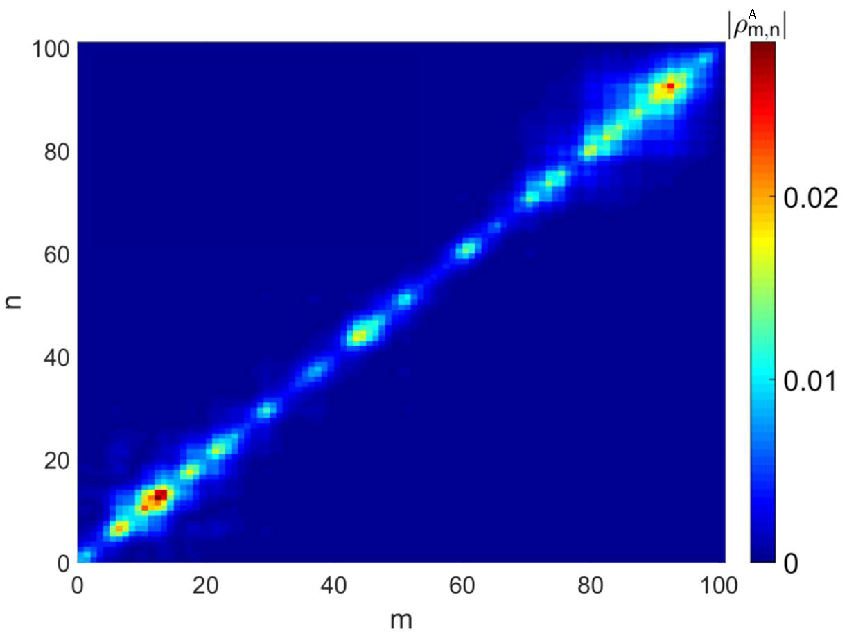
\includegraphics[width=0.5\linewidth]{anderson_rho_loc_1}}
		\hfill
		\subcaptionbox{\label{fig:anderson_rho_loc-2}}{%
			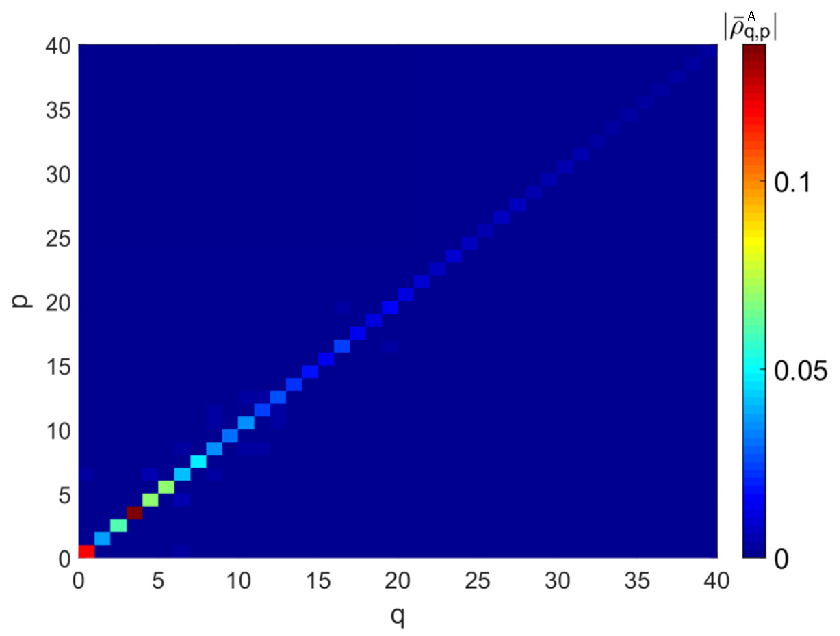
\includegraphics[width=0.5\linewidth]{anderson_rho_loc_2}}
		\hfill
	}
	\legend{}
	\caption[Асимптотическая матрица плотности с локализацией Андерсона]
	{
		Абсолютные значения асимптотической матрицы плотности \(\rho^A\) в исходном базисе (a) и в базисе собственных состояний модели Андерсона (б) для единичной реализации беспорядка. Использовались неэрмитовые диссипаторы \cref{eq:anderson_diss_local} c параметрами \(\alpha=0\) и \(l=1\). Сила пространственного беспорядка \(W=1\).
	}
	\label{fig:anderson_rho_loc}
\end{figure}

Зафиксируем параметры диссипаторов \(\alpha=0\) и \(l=1\) в формуле \cref{eq:anderson_diss_local} (синфазная диссипация на соседних сайтах решётки). В этом случае асимптотическая матрица плотности \(\rho^A\) имеет пятнистую структуру с несколькими яркими областями локализации, как показано на рисунке~\cref{fig:anderson_rho_loc-1}.
Рассмотрим асимптотическую матрицу плотности \(\rho^A\) в базисе собственных состояний модели Андерсона:
\begin{equation}
	\label{eq:anderson_rho_in_eigen_basis}
	\begin{gathered}
		\bar{\rho}^A = \mathcal{A}^\dagger \rho^A \mathcal{A},
	\end{gathered}
\end{equation}
где \(\mathcal{A} = \left(A_1 \ldots A_\nu \ldots A_N \right) \) "--- матрица собственных векторов гамильтониана \cref{eq:anderson_H}. В данном представлении матрица плотности \(\bar{\rho}^A\) является практически диагональной, с большим преобладанием значений из нижней части спектра, как показано на рисунке~\cref{fig:anderson_rho_loc-2}.

Для аналитического подтверждения данного наблюдения перепишем уравнение \cref{eq:GKSL_base} в базисе собственных состояний модели Андерсона \cref{eq:anderson_rho_in_eigen_basis}, пренебрегая недиагональными элементами матрицы плотности. В таком приближении эволюция диагональных элементов определяется только диссипативными членами:
\begin{equation}
	\label{eq:anderson_diag_mod_1}
	\begin{gathered}
		\dot{\bar{\rho}}_{p,p} = \gamma \left( \sum_q I_{p,q}\bar{\rho}_{q,q} - \bar{\rho}_{p,p} \sum_q I_{q,p} \right),
	\end{gathered}
\end{equation}
где коэффициенты перекрытий \(I_{p,q}\) представляются следующим образом через диссипативные операторы в базисе собственных состояний модели Андерсона (\(\bar{V}_k = \mathcal{A}^\dagger V_k \mathcal{A}\)):
\begin{equation}
	\label{eq:anderson_diag_mod_2}
	\begin{gathered}
		I_{p,q} = \sum_k \left| \left(\bar{V}_k\right)_{q,p} \right|^2 = \sum_k \left(\mathcal{A}_{p, k+l} + e^{i \alpha} \mathcal{A}_{p, k} \right)^2  \left(\mathcal{A}_{q, k+l} - e^{-i \alpha} \mathcal{A}_{q, k} \right)^2.
	\end{gathered}
\end{equation}
Система линейных дифференциальных уравнений \cref{eq:anderson_diag_mod_1} имеет единственное устойчивое состояние равновесия. Для его поиска, приравняем правую часть уравнения к \(0\), введём переобозначение:
\begin{equation}
	\label{eq:anderson_diag_mod_3}
	\begin{gathered}
		I^{\pm}_{p,k} = \left(\mathcal{A}_{p, k+l} \pm e^{\pm i \alpha} \mathcal{A}_{p, k} \right)^2 ,
	\end{gathered}
\end{equation}
и получим итоговое выражение для асимптотического состояния равновесия:
\begin{equation}
	\label{eq:anderson_diag_mod_4}
	\begin{gathered}
		\bar{\rho}^A_{p,p} = \frac{\sum_q I_{p,q}\bar{\rho}^A_{q,q}}{\sum_q I_{q,p}} = \frac{\sum_q \sum_k I^{+}_{p,k} I^{-}_{q,k} \bar{\rho}^A_{q,q}}{\sum_q \sum_k I^{+}_{q,k}  I^{-}_{p,k}} = \frac{\sum_k I^{+}_{p,k} \sum_q I^{-}_{q,k} \bar{\rho}^A_{q,q}}{ \sum_k I^{-}_{p,k} \sum_q  I^{+}_{q,k} } .
	\end{gathered}
\end{equation}
Внутренние суммы в числителе и знаменателе в самой правой части выражения не зависят от индекса \(p\). Они подвергаются усреднению по всем охватываемым собственным состояниям. Поскольку беспорядок пространственно однороден, среднее по ансамблю делает результат также независимым от индекса \(k\), и поэтому обе суммы соответствуют некоторой нормировочной константе. Таким образом, мы приходим к следующему выражению для асимптотической матрицы плотности в базисе собственных состояний модели Андерсона:
\begin{equation}
	\label{eq:anderson_diag_mod_5}
	\begin{gathered}
		\bar{\rho}^A_{p,p} \approx \frac{\sum_k I^{+}_{p,k}}{ \sum_k I^{-}_{p,k}}, 
	\end{gathered}
\end{equation}
которое полностью определяется типом диссипации и пространственной структурой конкретного собственного состояния.

Для случая синфазной диссипации на соседних сайтах решётки (\(\alpha=0\) и \(l=1\) в \cref{eq:anderson_diss_local}) получается соотношение:
\begin{equation}
	\label{eq:anderson_diag_mod_6}
	\begin{gathered}
		\sum_k \left( \mathcal{A}_{p, k+1} \pm \mathcal{A}_{p, k} \right)^2 = 2 \pm \sum_k \mathcal{A}_{p, k+1} \mathcal{A}_{p, k} = 2 \mp \lambda_p \mp \sum_k \varepsilon_k \mathcal{A}^2_{p, k}.
	\end{gathered}
\end{equation}
Оно основано на тождестве, полученном из следующего уравнения для собственных состояний:
\begin{equation}
	\label{eq:anderson_diag_mod_7}
	\begin{gathered}
		-\left( \lambda_p - \varepsilon_k \right) \mathcal{A}_{p, k} = \mathcal{A}_{p, k-1} + \mathcal{A}_{p, k+1},
	\end{gathered}
\end{equation}
которое, в свою очередь, умножается на \(\mathcal{A}_{p, k}\) и суммируется по \(k\).
В уравнении \cref{eq:anderson_diag_mod_6} в случае малого беспорядка (\(W < 4\)) и далеко от границ спектра, можно пренебречь последним слагаемым в правой части (усреднение из-за пространственного беспорядка), и в итоге получить следующее соотношение:
\begin{equation}
	\label{eq:anderson_diag_mod_8}
	\begin{gathered}
		\bar{\rho}^A_{p,p} \approx \frac{2-\lambda_p}{2+\lambda_p}.
	\end{gathered}
\end{equation}
Данный результат объясняет быстрое уменьшение вклада собственных состояний при отдалении от нижней границы спектра.
На рисунке~\cref{fig:anderson_rho_nn_1} для разных параметров силы беспорядка символами изображены усреднённые по многим реализация беспорядка распределения диагональных элементов асимптотической матрицы плотности в базисе собственных состояний модели Андерсона \(\bar{\rho}^A_{p,p}\) как функции усреднённых собственных значений. Количество реализаций беспорядка для усреднения: \(N_r=100\).
Полученные численные результаты хорошо согласуются с теоретической оценкой (формула \cref{eq:anderson_diag_mod_8} и фиолетовая кривая на рисунке~\cref{fig:anderson_rho_nn_1}). 
Несоответствие между результатами численных экспериментов и теоретической оценкой увеличивается с ростом силы беспорядка \(W\) и вблизи границ спектра "--- эти эффекты следуют из природы сделанных приближений.
\begin{figure}[ht]
	\centerfloat{
		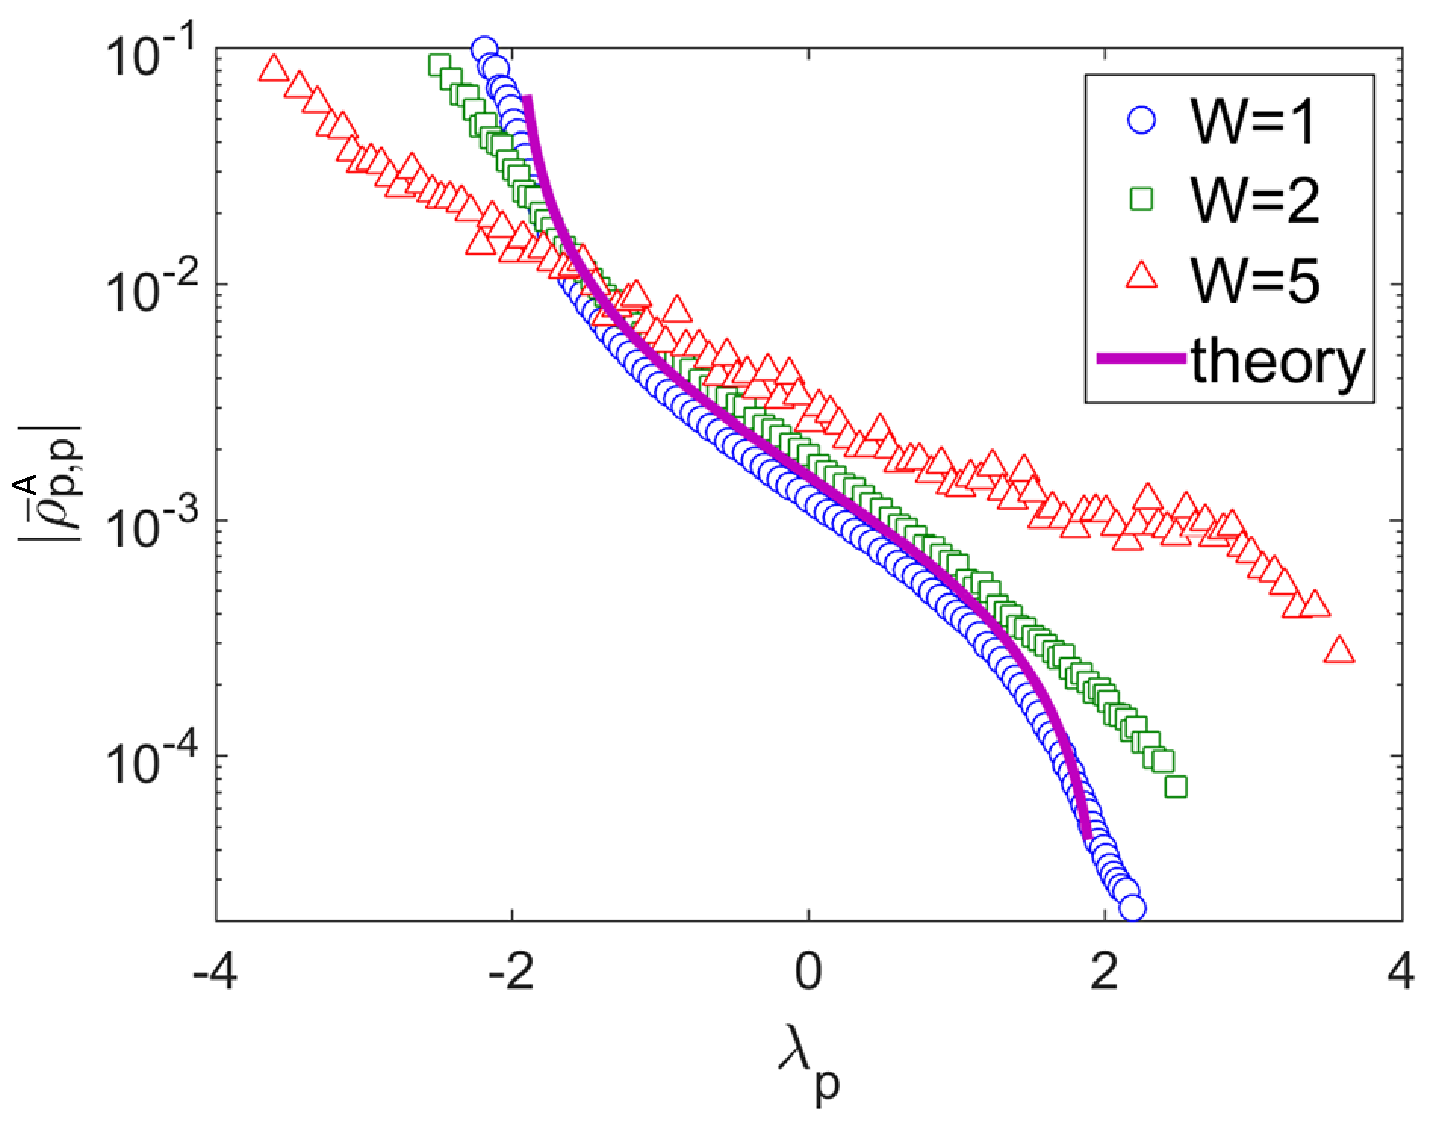
\includegraphics[scale=0.6]{anderson_rho_nn_1}
	}
	\caption[Усреднённые диагональные элементы матрицы плотности с локализацией Андерсона и теоретической оценкой]{
		Символы "--- усреднённые абсолютные значения диагональных элементов асимптотической матрицы плотности в базисе собственных состояний модели Андерсона как функции усреднённых собственных чисел для синфазной диссипации на соседних сайтах решётки (\(\alpha=0\) и \(l=1\) в уравнении \cref{eq:anderson_diss_local}) для разных значений беспорядка \(W\). Теоретический результат (формула \cref{eq:anderson_diag_mod_8}) показан фиолетовой сплошной линией.
	}
	\label{fig:anderson_rho_nn_1}
\end{figure}

Случай антифазной диссипации на соседних сайтах решетки (\(\alpha=\pi\) и \(l=1\) в уравнении \cref{eq:anderson_diss_local}), из-за симметрии, приводит к обратному выражению для формулы \cref{eq:anderson_diag_mod_8}:
\begin{equation}
	\label{eq:anderson_diag_mod_9}
	\begin{gathered}
		\bar{\rho}^A_{p,p} \approx \frac{2+\lambda_p}{2-\lambda_p}.
	\end{gathered}
\end{equation}
Асимптотическая матрица плотности является локализованной возле верхней границы спектра. 
При значениях фазы диссипации в промежутке \(0 < \alpha < \frac{\pi}{2}\)  в асимптотической матрице плотности в базисе собственных состояний модели Андерсона будут преобладать диагональные элементы, локализованные вблизи нижней границы спектра собственных значений. Аналогично, при значениях фазы диссипации в промежутке \(\frac{\pi}{2} < \alpha < \pi\) преобладают максимальные собственные значения из диапазона \cref{eq:anderson_evals}.

Качественно иная картина наблюдается для диссипативных операторов с \(\alpha=\pi\) и \(l=2\).
В этом случае асимптотическая матрица плотности в исходном базисе \(\rho^A\) является относительно более делокализованной (рисунок~\cref{fig:anderson_rho_loc-3}). 
В то же время, в базисе собственных состояний модели Андерсона \(\bar{\rho}^A\) \cref{eq:anderson_rho_in_eigen_basis} остаётся локализованной со смещением в центр спектра (рисунок~\cref{fig:anderson_rho_loc-4}).
\begin{figure}[ht]
	\centerfloat{
		\hfill
		\subcaptionbox[List-of-Figures entry]{\label{fig:anderson_rho_loc-3}}{%
			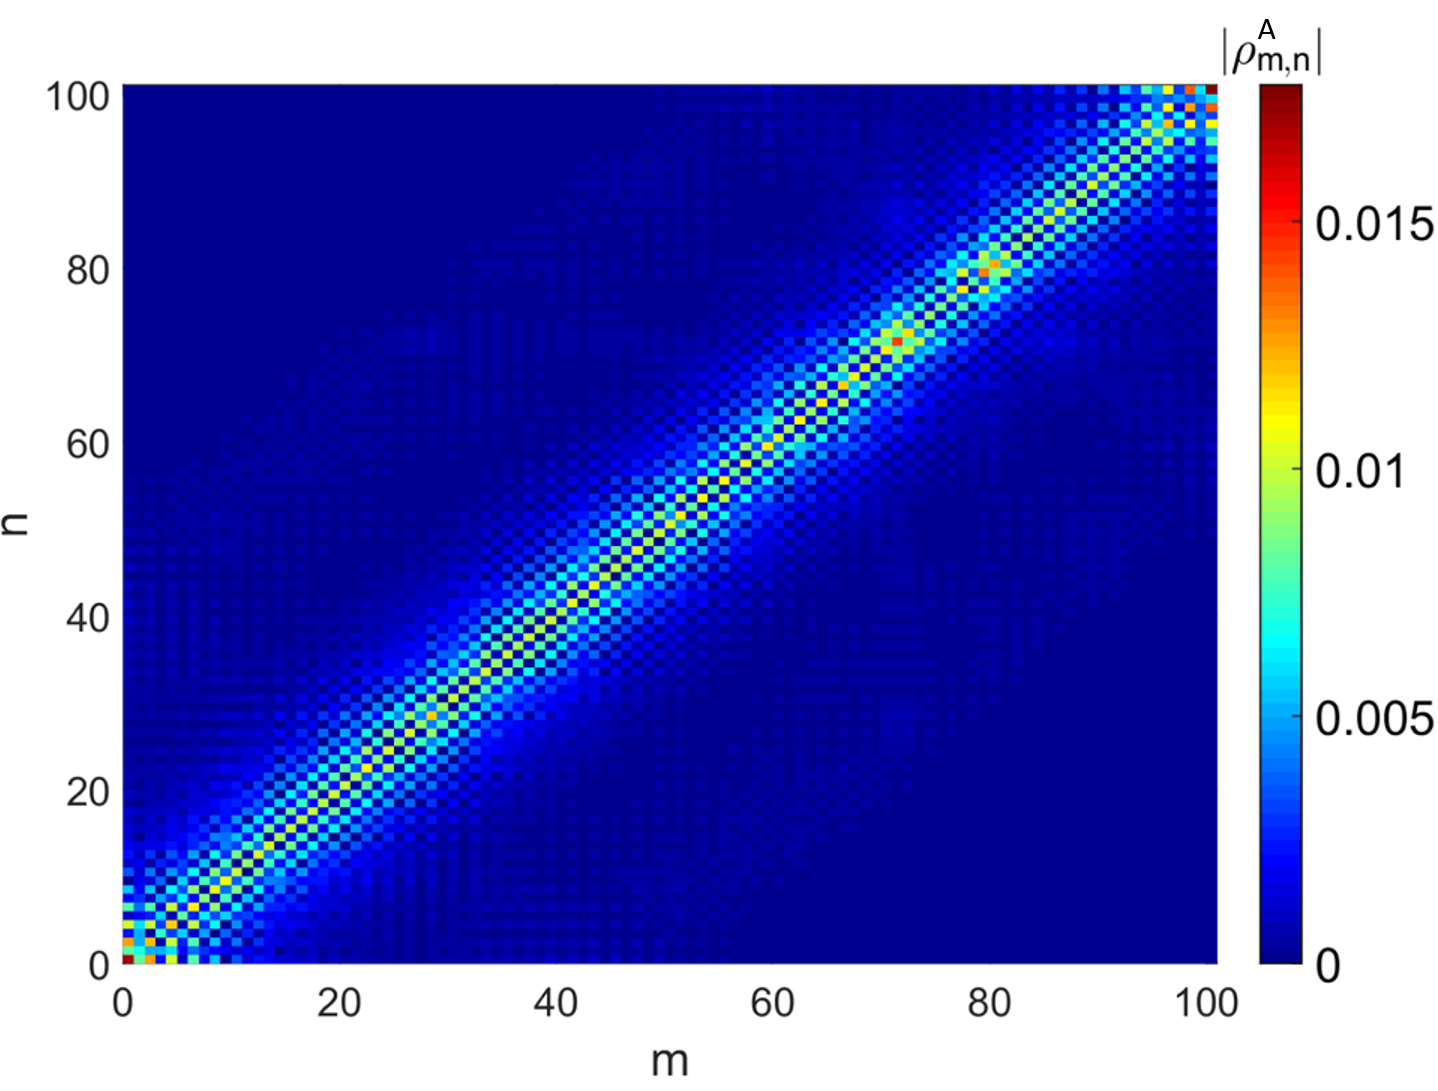
\includegraphics[width=0.5\linewidth]{anderson_rho_loc_3}}
		\hfill
		\subcaptionbox{\label{fig:anderson_rho_loc-4}}{%
			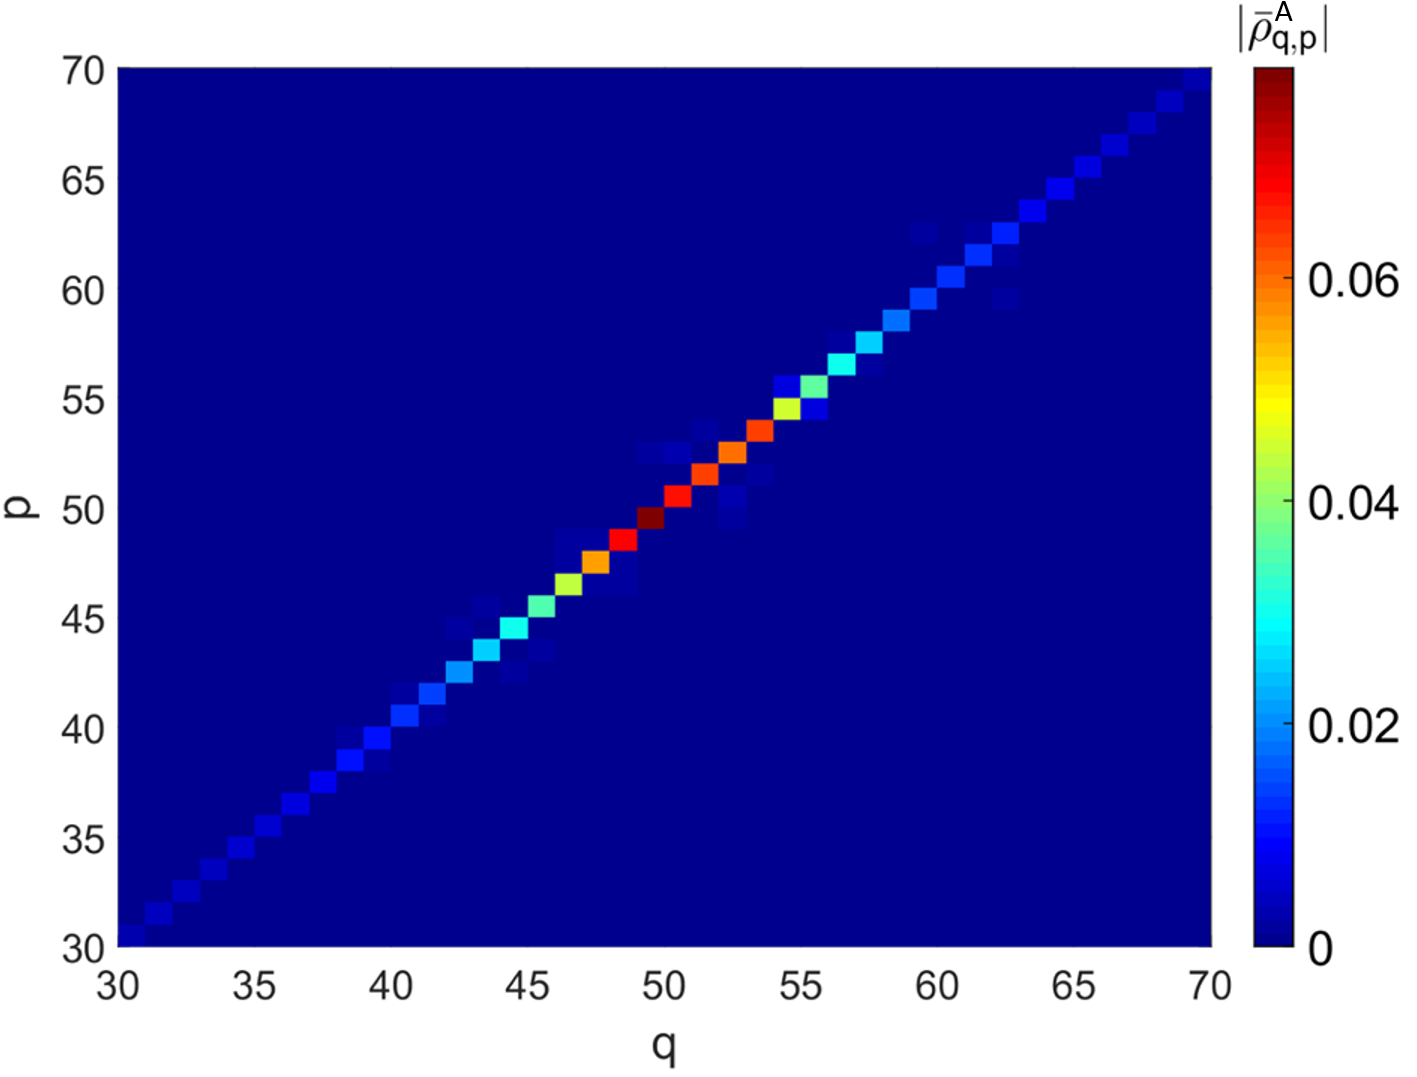
\includegraphics[width=0.5\linewidth]{anderson_rho_loc_4}}
		\hfill
	}
	\legend{}
	\caption[Асимптотическая матрица плотности с преобладанием делокализованных Андерсоновских мод]
	{
		Абсолютные значения асимптотической матрицы плотности \(\rho^A\) в исходном базисе (a) и в базисе собственных состояний модели Андерсона (б) для единичной реализации беспорядка. Использовались неэрмитовые диссипаторы \cref{eq:anderson_diss_local} c параметрами \(\alpha=\pi\) и \(l=2\). Сила пространственного беспорядка \(W=1\).
	}
	\label{fig:anderson_rho_loc_mid}
\end{figure}
Относительная делокализация в исходном базисе вызвана существенным вкладом собственных состояний из центра спектра, которые имеют относительно большую длину локализации \cref{eq:anderson_loc_length}.
Аналитические соотношения для данного случая выглядят следующим образом:
\begin{equation}
	\label{eq:anderson_diag_mod_10}
	\begin{gathered}
		I^{-}_p = \sum_{k} \left( \mathcal{A}_{p, k+2} \pm \mathcal{A}_{p, k} \right)^2 = \\
		= \lambda^2 - 2 \lambda_p \sum_{k} \varepsilon_k \mathcal{A}_{p, k} \mathcal{A}_{p, k+1} + \sum_{k} \varepsilon^2_k \mathcal{A}^2_{p, k} \approx \lambda^2_p + \frac{W^2}{12}, \\
		I^{+}_p = 4 - I^{-}_p,
	\end{gathered}
\end{equation}
которые в итоге приводят к следующему выражению для диагональных элементов матрицы плотности в базисе собственных состояний модели Андерсона:
\begin{equation}
	\label{eq:anderson_diag_mod_11}
	\begin{gathered}
		\bar{\rho}^A_{p,p} \approx \frac{4}{\lambda^2_p + \frac{W^2}{12}} - 1.
	\end{gathered}
\end{equation}
Данное выражение указывает на то, что наибольший вклад в решение вносят собственные состояния из центра спектра.
На рисунке \cref{fig:anderson_rho_nn_2} изображены усреднённые по \(N_r=100\) случайным реализациям беспорядка диагональные элементы матрицы плотности в базисе собственных состояний модели Андерсона для разных значений силы беспорядка вместе с аналитическим результатом \cref {eq:anderson_diag_mod_11} (сплошные линии). На графике видно хорошее соответствие между численными и аналитическими результатами при малом беспорядке \(W\). При увеличении \(W\) несоответствие увеличивается на краях спектра \(\lambda_p\) ввиду сделанных теоретических приближений. 
\begin{figure}[ht]
	\centerfloat{
		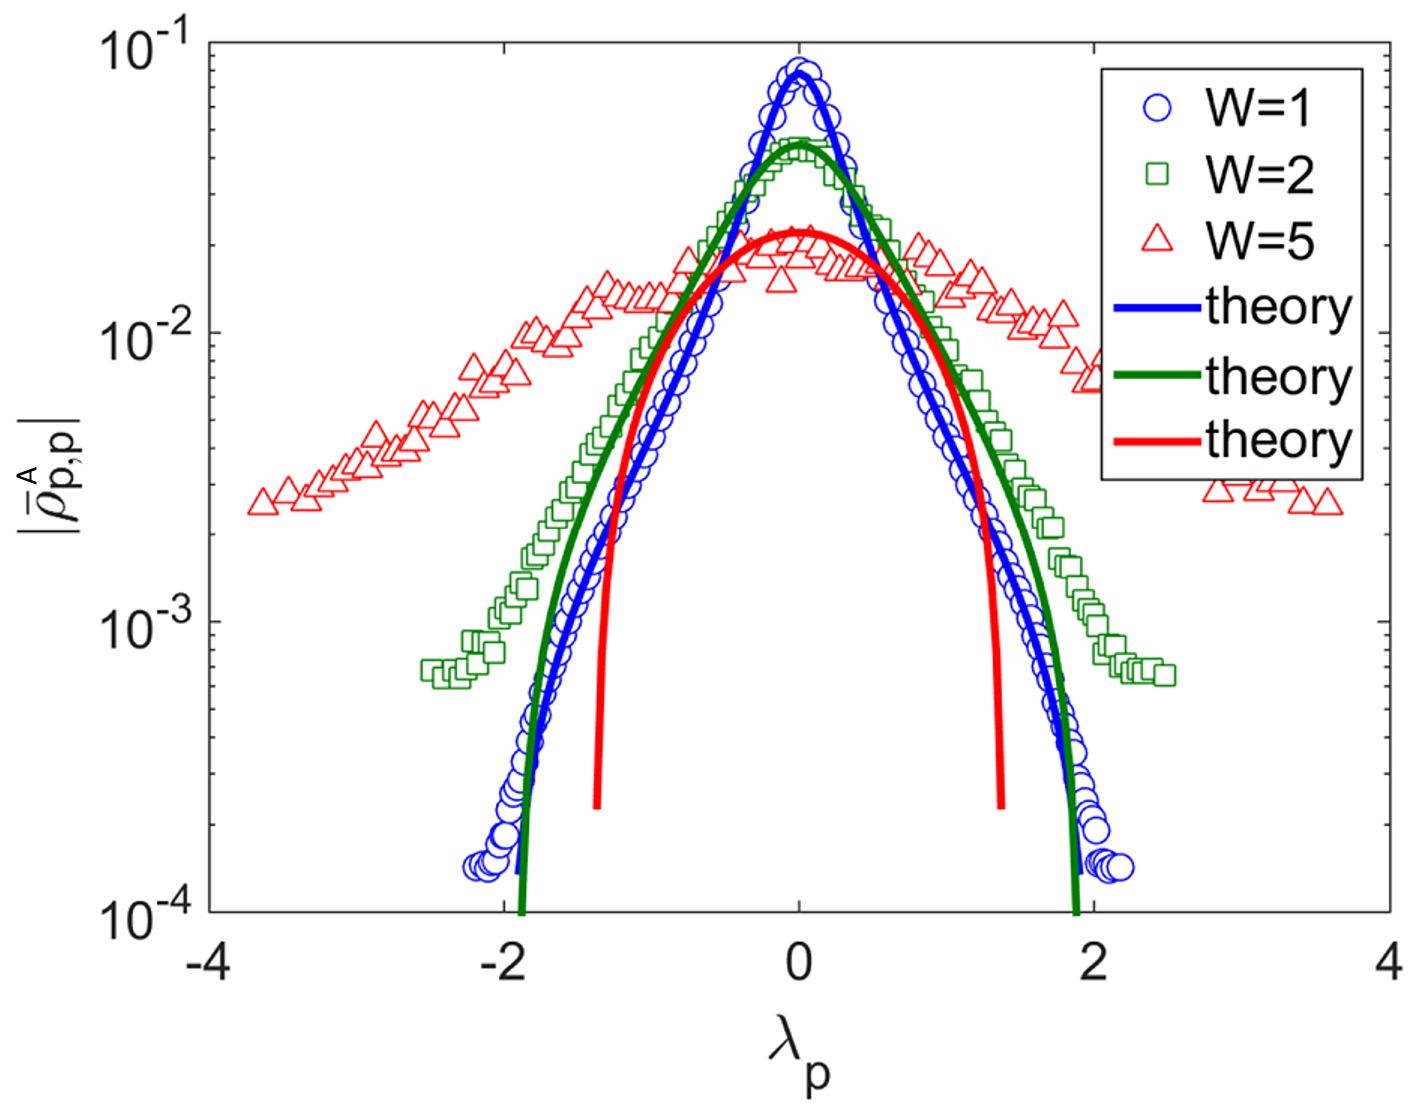
\includegraphics[scale=0.4]{anderson_rho_nn_2}
	}
	\caption[Усреднённые диагональные элементы матрицы плотности c преобладанием делокализованных Андерсоновских мод и теоретической оценкой]{
		Символы "--- усреднённые абсолютные значения диагональных элементов асимптотической матрицы плотности в базисе собственных состояний модели Андерсона как функции усреднённых собственных чисел для неэрмитовой диссипации  с \(\alpha=\pi\) и \(l=2\) в уравнении \cref{eq:anderson_diss_local} для разных значений беспорядка \(W\). Теоретический результат \cref{eq:anderson_diag_mod_11} для каждого значения \(W\) показан соответствующей сплошной линией.
	}
	\label{fig:anderson_rho_nn_2}
\end{figure}

Рассмотрим открытую модель Андерсона \cref{eq:GKSL_lindbladian, eq:anderson_H, eq:anderson_diss_local} c микроскопической точки зрения, используя метод квантовых тректорий, описанный в разделе \cref{sec:ch1/qj}. Квантовая траектория с индексом \(j\) будет описываться волновой функцией \(\left| \psi_j(t) \right\rangle\). Зафиксируем случайный беспорядок в системе силой \(W=1\) и время переходного процесса \(t^A = 10^4\) "--- достаточным до достижения каждой траекторией аттрактора (асимптотической матрицы плотности \(\rho^A\)). После достижения аттрактора за каждой квантовой траекторией будет вестись наблюдение в течении \(t^O = 10^4\) (суммарное время пропагации \(t = t^A + t^O\)). Количество рассматриваемых квантовых траекторий \(M_r=10^6\). Для каждой \(j\)-ой квантовой траектории будут рассматриваться позиция и энергия, вычисляемые по соответствующим формулам:
\begin{equation}
	\label{eq:anderson_position}
	\begin{gathered}
		n_j(t) = \langle \psi_j(t)| O_n | \psi_j(t) \rangle,
	\end{gathered}
\end{equation}
\begin{equation}
	\label{eq:anderson_energy}
	\begin{gathered}
		E_j(t) = \langle \psi_j(t)| H | \psi_j(t) \rangle,
	\end{gathered}
\end{equation}
где \(O_n\) - матрица оператора числа частиц, а \(H\) - гамильтониан модели Андерсона \cref{eq:anderson_H}.

\begin{figure}[ht]
	\centerfloat{
		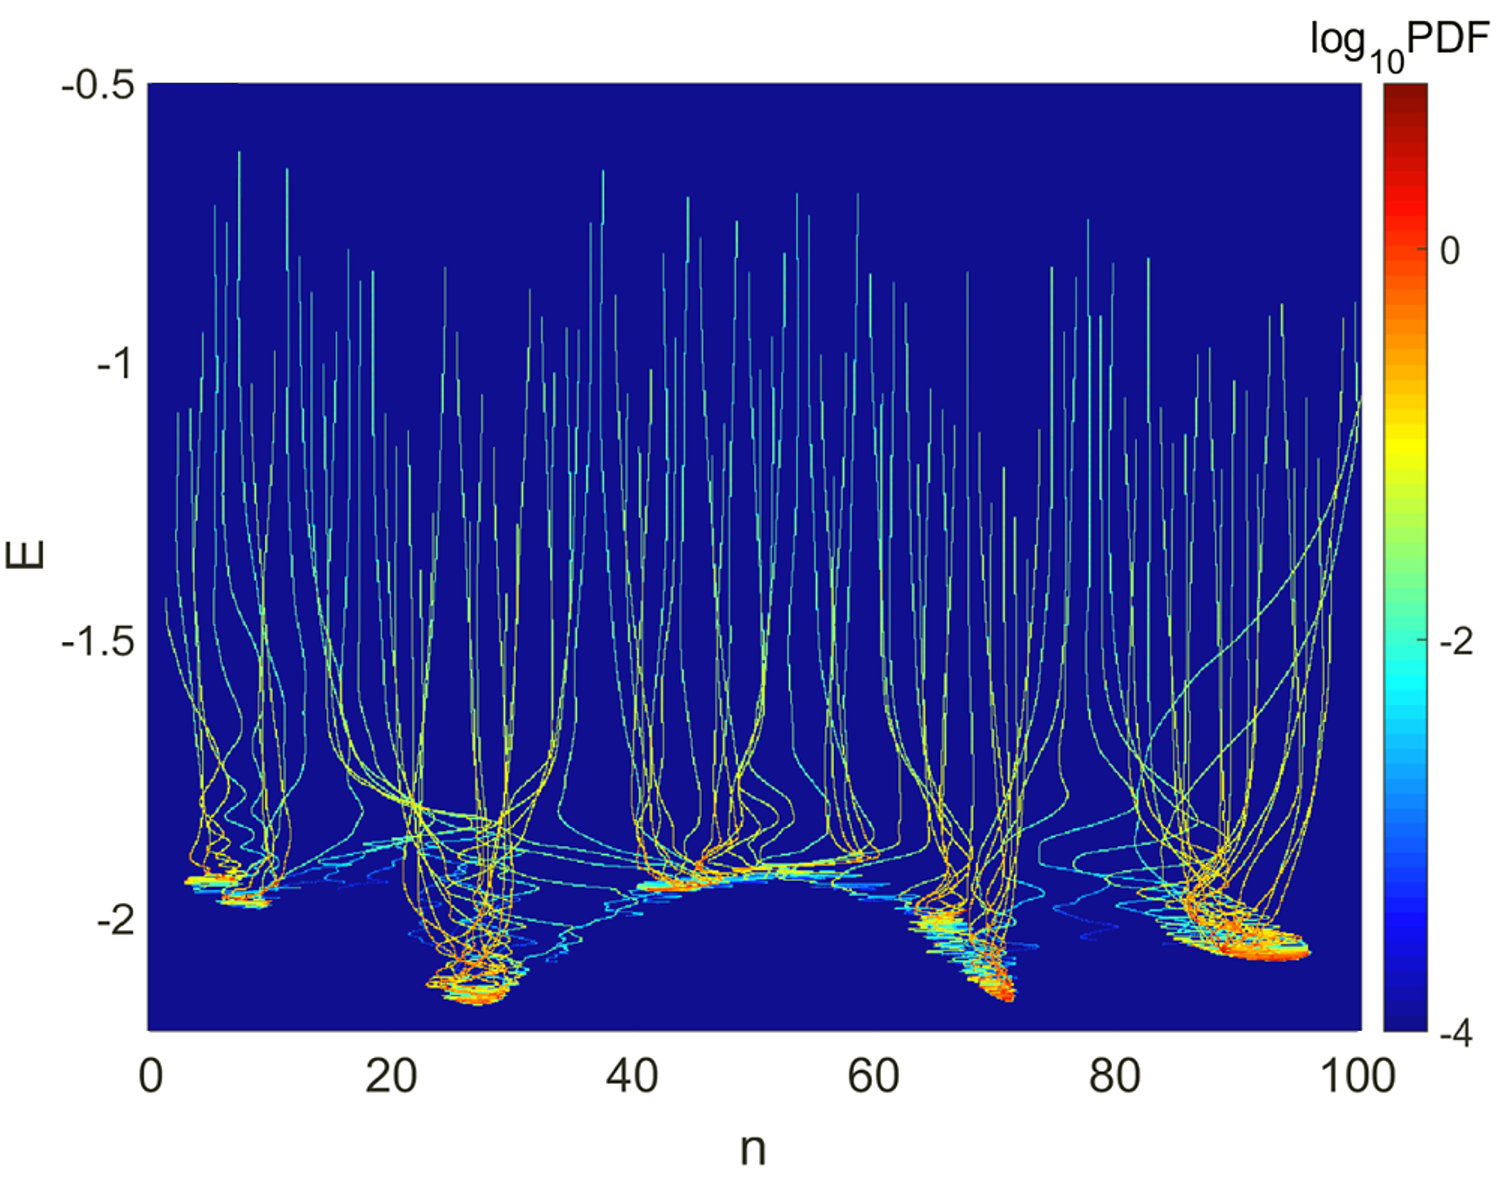
\includegraphics[scale=0.4]{anderson_qj_1}
	}
	\caption[Плотность вероятностей квантовых траекторий на плоскости позиции и энергий в случае  локализации Андерсона]{
		Функция распределения плотности вероятностей (PDF) квантовых траекторий на плоскости позиции \(n(t)\) и энергии \(E(t)\) для случая синфазной диссипации на соседних сайтах решётки (\(\alpha=0\) и \(l=1\) в \cref{eq:anderson_diss_local}).
	}
	\label{fig:anderson_qj_1}
\end{figure}

На рисунке \cref{fig:anderson_qj_1} изображена двумерная функция распределения плотности вероятностей (probability densidy function - PDF) на плоскости позиции \(n(t)\) \cref{eq:anderson_position} и энергии \(E(t)\) \cref{eq:anderson_energy} , построенная для \(M_r=10^6\) траекторий, наблюдаемых в течение \(t^O=10^4\) времени для случая синфазной диссипации на соседних сайтах решётки (\(\alpha=0\) и \(l=1\) в \cref{eq:anderson_diss_local}). Динамика отдельных квантовых траекторий представляет собой длительные «залипания» вблизи центров локализации (красные области на рисунке \cref{fig:anderson_qj_1}), вызванные эволюцией с неэрмитовым гамильтонианом \cref{eq:H_nonhermit} (алгоритм \ref{alg:qt_main}). Данные процессы прерываются квантовыми скачками (алгоритм \ref{alg:qt_jump}), которые накачивают систему энергией и переносят траектории в бледно-голубые «истоки» сети в верхней части рисунка \cref{fig:anderson_qj_1}, откуда системы быстро релаксирует по структурированной сети к одному из собственных состояний модели Андерсона. Структура сети не меняется при дальнейшем увеличении числа траекторий \(M_r\).

Результаты \cite{Yusipov2017}, представленные в данном разделе, указывают на то, что в открытых квантовых системах с физически реализуемой диссипацией возможно создание стационарных состояний, в которых доминируют несколько локализованных мод пространственно неоднородного гамильтониана из классической модели Андерсона. Андерсоновские моды выбираются в соответствии с их пространственно-фазовыми свойствами, унаследованными от собственных состояний гамильтониана в пределе нулевого беспорядка \cite{Ishii1973}, с использованием фазо"--~параметризованных диссипативных операторов. Изменение фазы диссипативных операторов изменяет локализационные свойства системы.

\section{Управление одночастичной локализацией в открытых квантовых системах}\label{sec:ch2/epjb}
В данном разделе будет изучено влияние параметров диссипативных операторов \cref{eq:anderson_diss_local} на локализационные свойства открытой квантовой системы \cref{eq:GKSL_lindbladian,eq:anderson_H}, а также влияние добавочной дефазирующей диссипации \cref{eq:anderson_diss_dephase} на асимптотическое состояние системы.

Рассмотрим случай синфазной диссипации на соседних сайтах решётки (\(\alpha=0\) и \(l=1\) в \cref{eq:anderson_diss_local} с коэффициентами скорости диссипации \(\gamma^l = 0.1\). Добавим к данной модели дополнительные дефазирующие \cref{eq:anderson_diss_dephase} каналы рассеивания с коэффициентами скорости \(\gamma^d\). На рисунке \cref{fig:anderson_rho_nn_with_dephasing} изображены диагональные элементы асимптотической матрицы плотности в базисе собственных состояний модели Андерсона со смешанным типом диссипации для разных значений \(\gamma^d\). Стоить отметить, что не только слабая \(\gamma^d \ll \gamma^l\), но и сильная \(\gamma^d \gg \gamma^l\) дефазирующая диссипация не уничтожает спектральную диссипацию и структурно не изменяет решение (преобладают собственные состояния из той же части спектра).

\begin{figure}[ht]
	\centerfloat{
		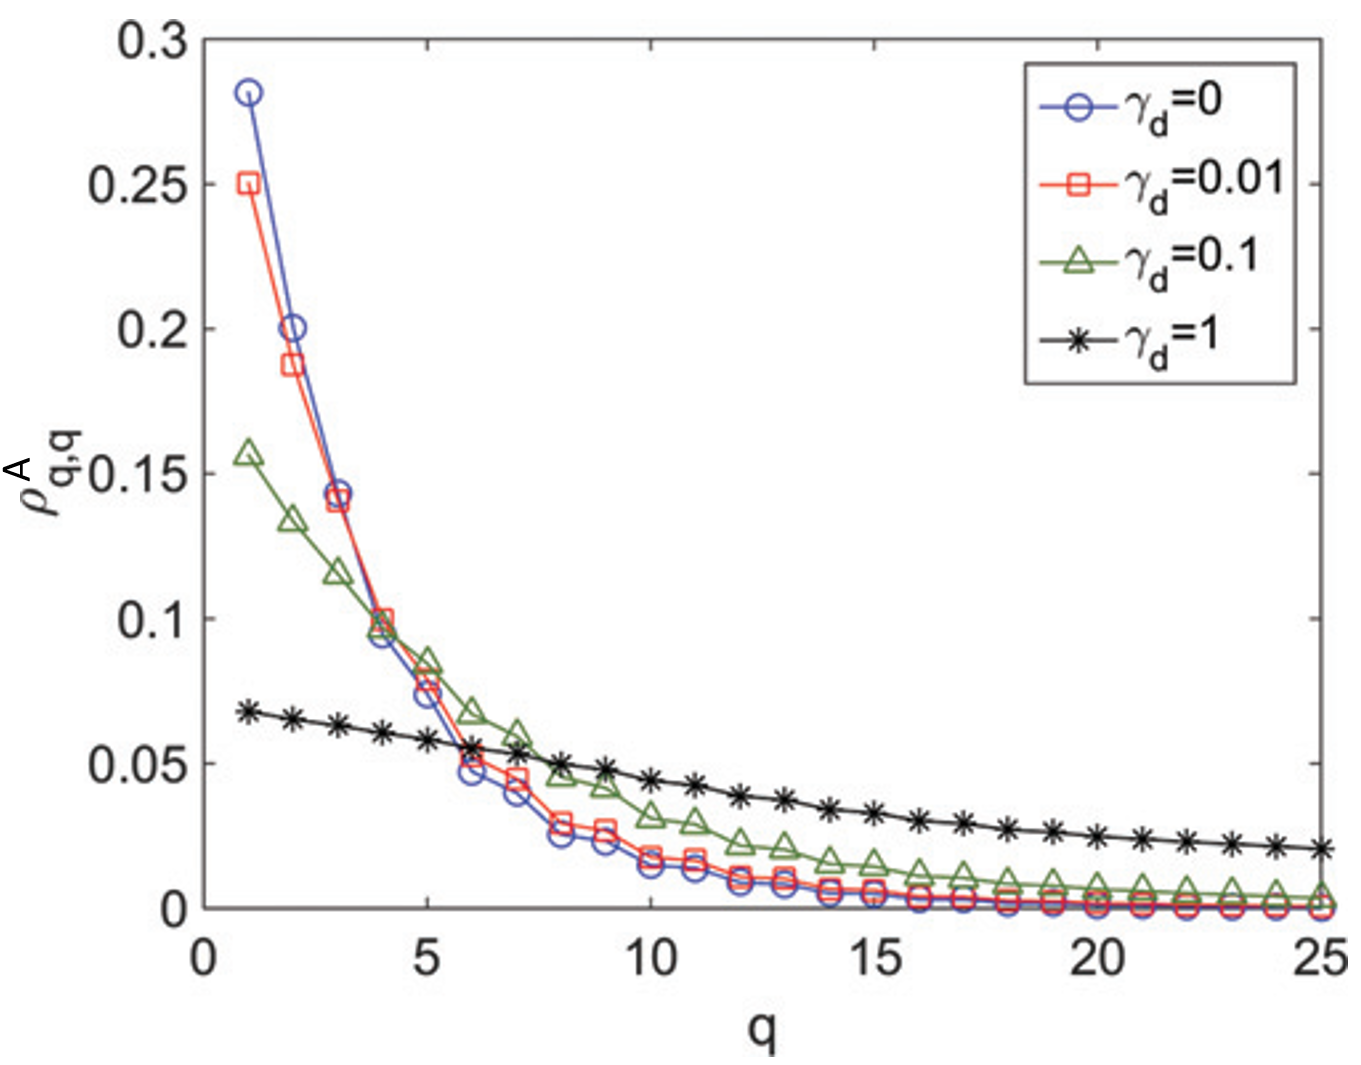
\includegraphics[scale=0.4]{anderson_rho_nn_with_dephasing}
	}
	\caption[Диагональные элементы асимптотической матрицы плотности в базисе собственных состояний модели Андерсона для разных типов диссипации]{
		Диагональные элементы асимптотической матрицы плотности в базисе собственных состояний модели Андерсона \(\bar{\rho}^A\) для случая синфазной диссипации на соседних сайтах решётки (\(\alpha=0\) и \(l=1\) в \cref{eq:anderson_diss_local} и скорость диссипации \(\gamma^l=0.1\)) в комбинации с дефазирующей диссипацией (\cref{eq:anderson_diss_dephase} и скорость диссипации \(\gamma^d\)) для разных значений \(\gamma^d\). Размер решётки \(N=25\), сила пространственного беспорядка \(W=2\). Усреднение производилось для \(N_r = 10^3\) реализаций беспорядка. 
	}
	\label{fig:anderson_rho_nn_with_dephasing}
\end{figure}

Рассмотрим теперь систему в пределе нулевого беспорядка. Базис системы состоит из плоских волн с соответсвующим спектром собственных значений:
\begin{equation}
	\label{eq:anderson_plane_wave}
	\begin{gathered}
		\phi_j = \frac{e^{i j k}}{\sqrt{N}}, \\
		\lambda_k = -2 \cos{k}, \\
		k = \frac{2 \pi q}{N}, \\
		q = -\frac{N}{2}, \ldots, \frac{N}{2}.
	\end{gathered}
\end{equation}
Можно заметить, что для конкретного значения фазы диссипатора \cref{eq:anderson_diss_local} \(\alpha = \frac{2 \pi q}{N}\), плоская волна  \cref{eq:anderson_plane_wave} с соответствующим \(k=\alpha\) является «тёмным» состоянием для всех диссипативных операторов \cref{eq:anderson_diss_local} \cite{Diehl2008, Kraus2008}, в то время как все остальные собственные состояния не являются.
В этом случае (когда нет дефазирующей добавки \(\gamma^d = 0\)), плоская волна с \(k = \alpha\) является асимптотическим состоянием открытой квантовой системы. 
В том случае, когда \(\alpha\) не совпадает точно со значением \(k\) или присутствует дефазирующая диссипация, асимптотическое состояние остаётся очень близким к исходному «тёмному» состоянию, причём наибольший вклад вносят плоские волны с \(k \approx \alpha\) (рисунок \cref{fig:anderson_rho_nn_zero_disorder}).
\begin{figure}[ht]
	\centerfloat{
		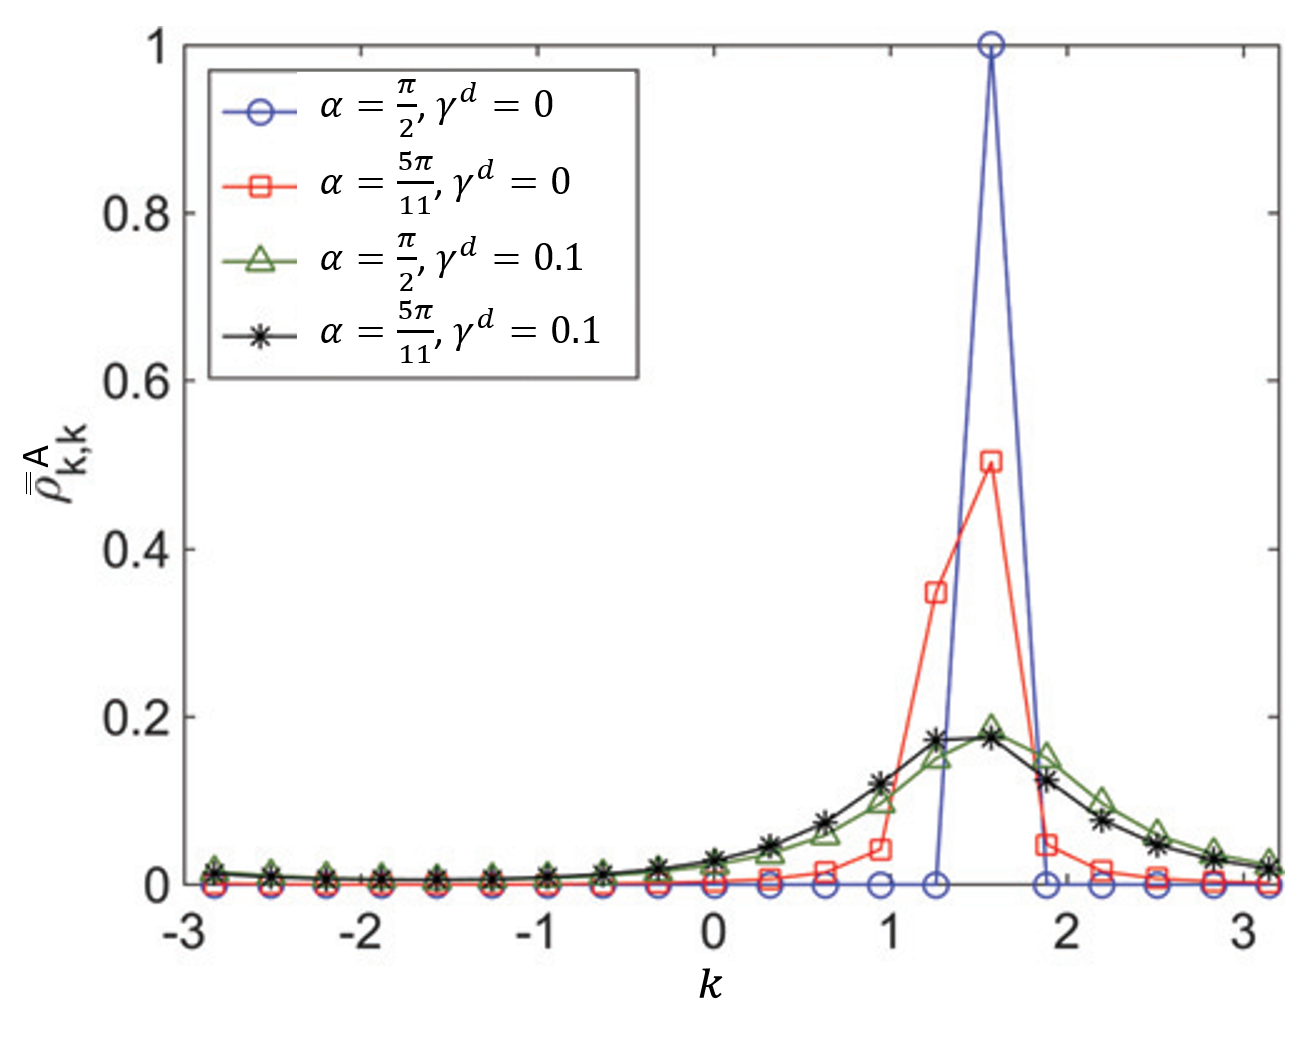
\includegraphics[scale=0.4]{anderson_rho_nn_zero_disorder}
	}
	\caption[Диагональные элементы асимптотической матрицы плотности в базисе Андерсоновских мод при нулевом беспорядке в зависимости от разных типов диссипации]{
		Диагональные элементы асимптотической матрицы плотности в базисе плоских волн \(\bar{\bar{\rho}}^A_{k,k}\) \cref{eq:anderson_plane_wave} для случая синфазной диссипации на соседних сайтах решётки (\(\alpha=0\) и \(l=1\) в \cref{eq:anderson_diss_local} и скорость диссипации \(\gamma^l=0.1\)) в комбинации с дефазирующей диссипацией (\cref{eq:anderson_diss_dephase} и скорость диссипации \(\gamma^d\)). Размер решётки \(N=20\), сила пространственного беспорядка \(W=0\).
	}
	\label{fig:anderson_rho_nn_zero_disorder}
\end{figure}

Ненулевой беспорядок \(W\) приводит к локализации Андерсона всех собственных состояний данной модели, которые при этом перестают в точности быть «тёмными» состояниями соответствующих диссипаторов \cref{eq:anderson_diss_local}.
Однако, известно, что моды Андерсона наследуют фазовые свойства исходных плоских волн (по крайней мере, в режиме слабого беспорядка), хотя их амплитуды экспоненциально затухают в пространстве \cite{Ishii1973}.
Следовательно, избирательный эффект неэрмитовых диссипаторов \cref{eq:anderson_diss_local} сохраняется.
\begin{figure}[h]
	\centerfloat{
		\hfill
		\subcaptionbox[List-of-Figures entry]{\label{fig:anderson_modes_in_foutier_1_1}}{%
			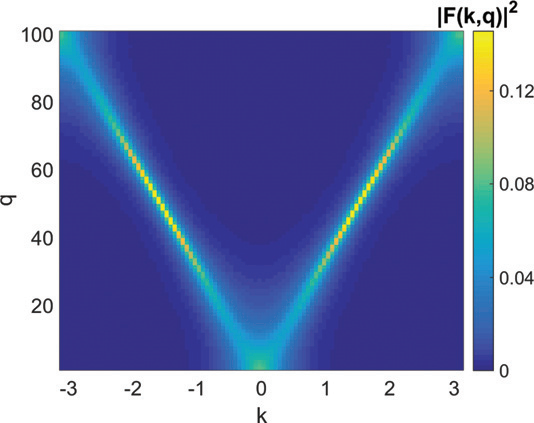
\includegraphics[width=0.45\linewidth]{anderson_modes_in_fourier_1_1}}
		\hfill
		\subcaptionbox{\label{fig:anderson_modes_in_foutier_1_2}}{%
			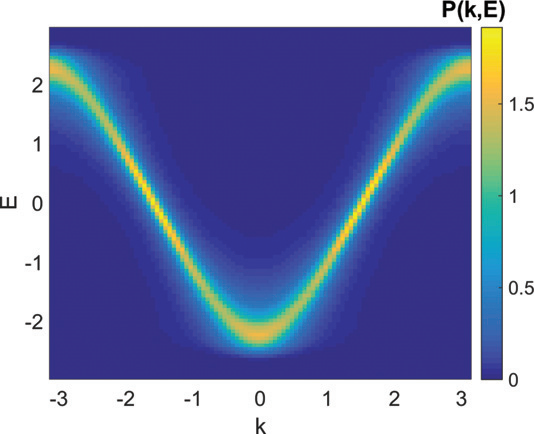
\includegraphics[width=0.45\linewidth]{anderson_modes_in_fourier_1_2}}
		\hfill
	}
	\legend{}
	\caption[Анализ Андерсоновских мод в Фурье"--~базисе для слабого беспорядка]
	{
		Собственные состояния модели Андерсона (Андерсоновские моды) с беспорядком \(W=2\) в Фурье"--~базисе плоских волн \cref{eq:anderson_modes_in_plane_wave}. (а): квадрат значения гармоник \(\left| F(k,q) \right|^2\) в зависимости от волнового числа \(k\) и номера моды \(q\); (б): значения спектральной плотности \(P(k,E)\) \cref{eq:anderson_modes_in_plane_wave_density}.
	}
	\label{fig:anderson_modes_in_foutier_1}
\end{figure}
\begin{figure}[h]
	\centerfloat{
		\hfill
		\subcaptionbox[List-of-Figures entry]{\label{fig:anderson_modes_in_foutier_2_1}}{%
			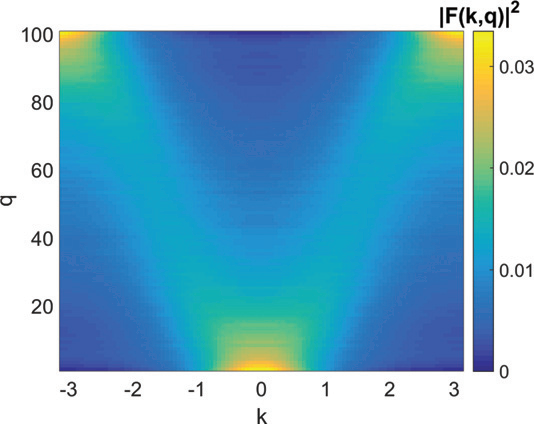
\includegraphics[width=0.45\linewidth]{anderson_modes_in_fourier_2_1}}
		\hfill
		\subcaptionbox{\label{fig:anderson_modes_in_foutier_2_2}}{%
			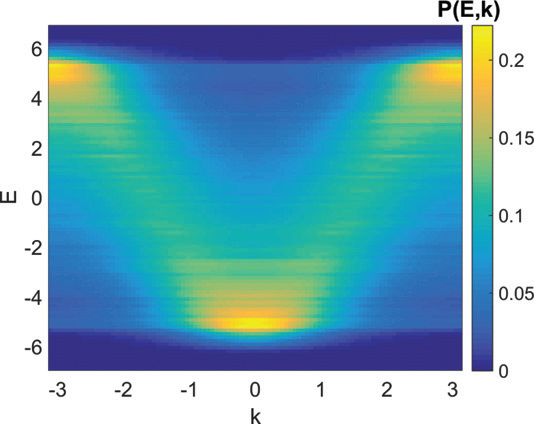
\includegraphics[width=0.45\linewidth]{anderson_modes_in_fourier_2_2}}
		\hfill
	}
	\legend{}
	\caption[Анализ Андерсоновских мод в Фурье"--~базисе для сильного беспорядка]
	{
		Собственные состояния модели Андерсона (Андерсоновские моды) с беспорядком \(W=10\) в Фурье"--~базисе плоских волн \cref{eq:anderson_modes_in_plane_wave}. (а): квадрат значения гармоник \(\left| F(k,q) \right|^2\) в зависимости от волнового числа \(k\) и номера моды \(q\); (б): значения спектральной плотности \(P(k,E)\) \cref{eq:anderson_modes_in_plane_wave_density}.
	}
	\label{fig:anderson_modes_in_foutier_2}
\end{figure}
\begin{figure}[h]
	\centerfloat{
		\hfill
		\subcaptionbox[List-of-Figures entry]{\label{fig:anderson_rho_kk_in_foutier_1_1}}{%
			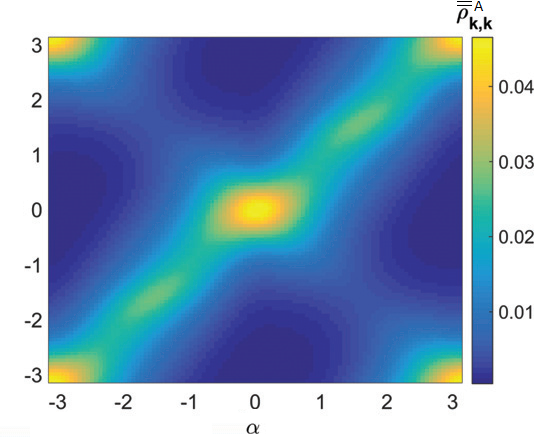
\includegraphics[width=0.45\linewidth]{anderson_rho_kk_in_foutier_1_1}}
		\hfill
		\subcaptionbox{\label{fig:anderson_rho_kk_in_foutier_1_2}}{%
			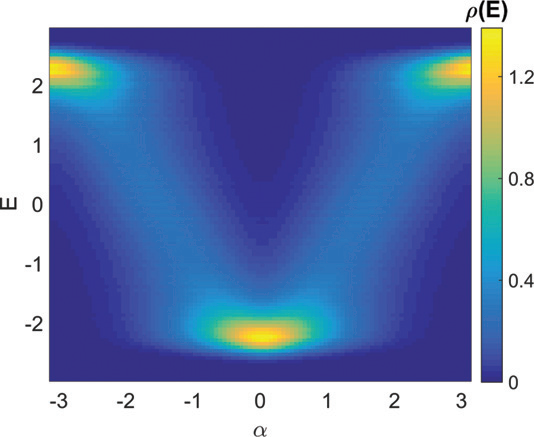
\includegraphics[width=0.45\linewidth]{anderson_rho_kk_in_foutier_1_2}}
	}
	\legend{}
	\caption[Асимптотическое состояние открытой системы Андерсона для слабого беспорядка в зависимости от параметра диссипации]
	{
		Асимптотическое состояние открытой системы Андерсона с беспорядком \(W=2\) и усреднением по \(N_r=10^3\) реализаций беспорядка в зависимости от параметра диссипации \(\alpha\) (\cref{eq:anderson_diss_local}). (а): диагональные элементы асимптотической матрицы плотности в базисе плоских волн \(\rho^A_{k,k}\) \cref{eq:anderson_plane_wave} ; (б): спектральная плотность диагональных элементов матрицы плотности в базисе собственных состояний модели Андерсона.
	}
	\label{fig:anderson_rho_kk_in_foutier_1}
\end{figure}
\begin{figure}[h]
	\centerfloat{
		\hfill
		\subcaptionbox[List-of-Figures entry]{\label{fig:anderson_rho_kk_in_foutier_2_1}}{%
			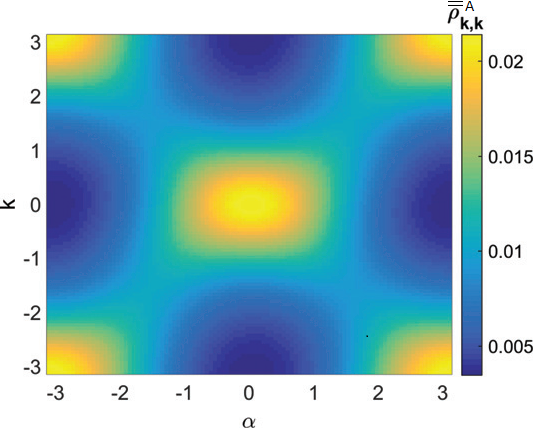
\includegraphics[width=0.45\linewidth]{anderson_rho_kk_in_foutier_2_1}}
		\hfill
		\subcaptionbox{\label{fig:anderson_rho_kk_in_foutier_2_2}}{%
			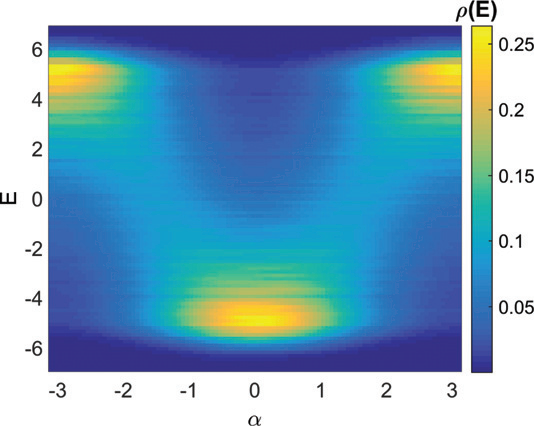
\includegraphics[width=0.45\linewidth]{anderson_rho_kk_in_foutier_2_2}}
	}
	\legend{}
	\caption[Асимптотическое состояние открытой системы Андерсона для сильного беспорядка в зависимости от параметра диссипации]
	{
		Асимптотическое состояние открытой системы Андерсона с беспорядком \(W=10\) и усреднением по \(N_r=10^3\) реализаций беспорядка в зависимости от параметра диссипации \(\alpha\) (\cref{eq:anderson_diss_local}). (а): диагональные элементы асимптотической матрицы плотности в базисе плоских волн \(\rho^A_{k,k}\) \cref{eq:anderson_plane_wave} ; (б): спектральная плотность диагональных элементов матрицы плотности в базисе собственных состояний модели Андерсона.
	}
	\label{fig:anderson_rho_kk_in_foutier_2}
\end{figure}

Зафиксируем параметры системы \(\gamma^l = \gamma^d = 0.1\), \(N=100\) и проанализируем структуру Андерсоновских мод \(A^{q}_k\) в базисе плоских волн \cref{eq:anderson_plane_wave} (Фурье"--~базис) для разных значений силы беспорядка \(W\).
Несмотря на то, что экспоненциальная локализация в прямом пространстве предполагает делокализацию в базисе плоских волн, она не исключает неоднородности распределения в нем.
Коэффициенты разложения, которые выражаются следующим образом:
\begin{equation}
	\label{eq:anderson_modes_in_plane_wave}
	\begin{gathered}
		F(k,q) = \sum A^q_k \frac{e^{i j k}}{\sqrt{N}},
	\end{gathered}
\end{equation}
имеют ярко выраженные максимумы вдоль линейных зависимостей \(q \approx \pm k_{max}\), как показано на рисунке \cref{fig:anderson_modes_in_foutier_1_1}.
Также была вычислена спектральная плотность коэффициентов разложения:
\begin{equation}
	\label{eq:anderson_modes_in_plane_wave_density}
	\begin{gathered}
		P(k,E) = \lim_{\Delta E \to 0} \frac{1}{\Delta E} \sum_{q:E(q) \in [E, E + \Delta E]} \left| F(k,q) \right|^2 ,
	\end{gathered}
\end{equation}
которая воспроизводит дисперсионное соотношение (рисунок \cref{fig:anderson_modes_in_foutier_1_2}).
Примечательно, что эти особенности присутствуют даже в режиме сильного беспорядка \(W=10\) (рисунок \cref{fig:anderson_modes_in_foutier_2_1, fig:anderson_modes_in_foutier_2_2}).

Связь между пространственной структурой мод Андерсона и их положением в спектре даёт ключ к пониманию способа выбора мод для формирования асимптотического состояния. Очевидно, это можно сделать, варьируя фазовый параметр \(\alpha\) неэрмитовых диссипаторов \cref{eq:anderson_diss_local}.
Численные результаты показывают хорошо очерченный максимум диагональных элементов асимптотической матрицы плотности в базисе плоских волн \(\bar{\bar{\rho}}^A_{k,k}\), такой, что \(k_{max} \approx \alpha\) (рисунок \cref{fig:anderson_rho_kk_in_foutier_1_1}). Также была вычислена спектральная плотность диагональных элементов матрицы плотности в базисе собственных состояний модели Андерсона \cref{eq:anderson_rho_in_eigen_basis}:
\begin{equation}
	\label{eq:anderson_rho_kk_density}
	\begin{gathered}
		\varrho(E) = \lim_{\Delta E \to 0} \frac{1}{\Delta E} \sum_{q:E(q) \in [E, E + \Delta E]} \bar{\rho}^A_{q,q},
	\end{gathered}
\end{equation}
проиллюстрированная на рисунке \cref{fig:anderson_rho_kk_in_foutier_1}. Точно так же, хотя и с менее чёткими границами воспроизводятся все результаты для случая сильного беспорядка \(W=10\) (рисунок \cref{fig:anderson_rho_kk_in_foutier_2}).

Таким образом, было продемонстрировано, что синтетическая диссипация может использоваться для управления свойствами локализации асимптотических состояний одночастичных квантовых систем. Механизм управления основан на фазовых свойствах локализованных мод гамильтониана системы Андерсона, которые являются  «тёмными» (либо близкими к «тёмным») состояниями синтетических диссипаторов \cite{Vershinina2017}.

\section{Распространение волновых пакетов в открытых квантовых системах с локализацией}\label{sec:ch2/prb_jump}
В данном разделе изучаются режимы распространения волновых пакетов квантовых траекторий \cite{Dalibard1992, Dum1992, Plenio1998} (раздел \cref{sec:ch1/qj}) в открытой модели Андерсона (раздел \cref{sec:ch1/sec3}). Также будет рассмотрена статистика времён между последовательными квантовыми скачками для разных режимов распространения.

Зафиксируем общий случай параметров модели в рамках данного раздела (если нет дополнительных уточнений): размер решётки \(N=200\), количество квантовых траекторий для усреднения \(M_r=10^3\), сила пространственного беспорядка \(W=1\), время переходного процесса для достижения аттрактора \(t^A = \frac{10^3}{\gamma}\), время наблюдения за квантовыми траекториями на аттракторе \(t^O = 10^7\) (общее время интегрирования равно \(t^A + t^O\)) и периодические граничные условия \(\rho_0 = \rho_{N+1}\). Используются неэрмитовые диссипаторы \cref{eq:anderson_diss_local} с разными значениями фазы \(\alpha\) и, как контрольный случай, дефазирующие диссипаторы \cref{eq:anderson_diss_dephase}.

Асимптотическая матрица плотности \(\rho^A\) описывает статистическое распределение единичных квантовых траекторий, но не содержит информации о микроскопической динамике в асимптотическом режиме. Для данного типа анализа применяется метод квантовых траекторий, описанный в разделе \cref{sec:ch1/qj}.

\begin{figure}[ht]
	\centerfloat{
		\hfill
		\subcaptionbox[List-of-Figures entry]{\label{fig:anderson_prb_1_1}}{%
			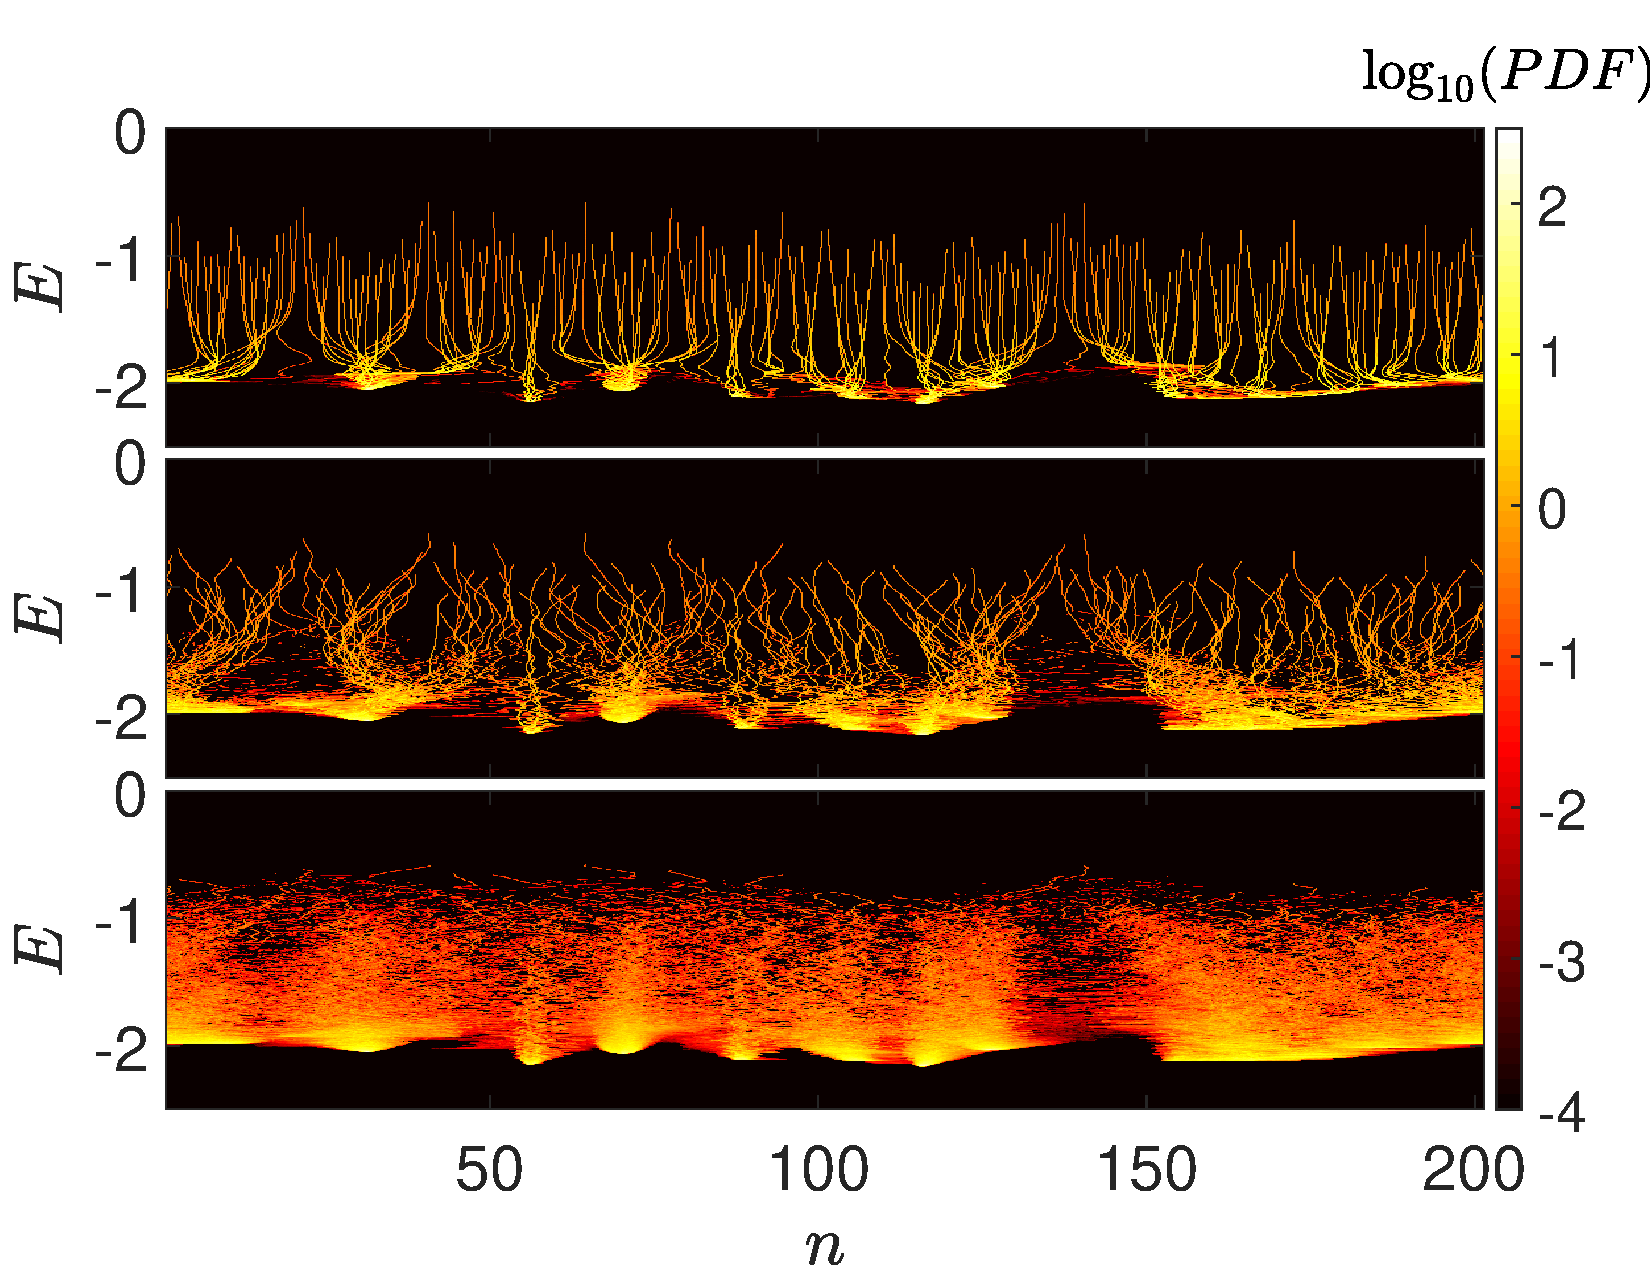
\includegraphics[width=0.5\linewidth]{anderson_prb_1_1}}
		\hfill
		\subcaptionbox{\label{fig:anderson_prb_1_2}}{%
			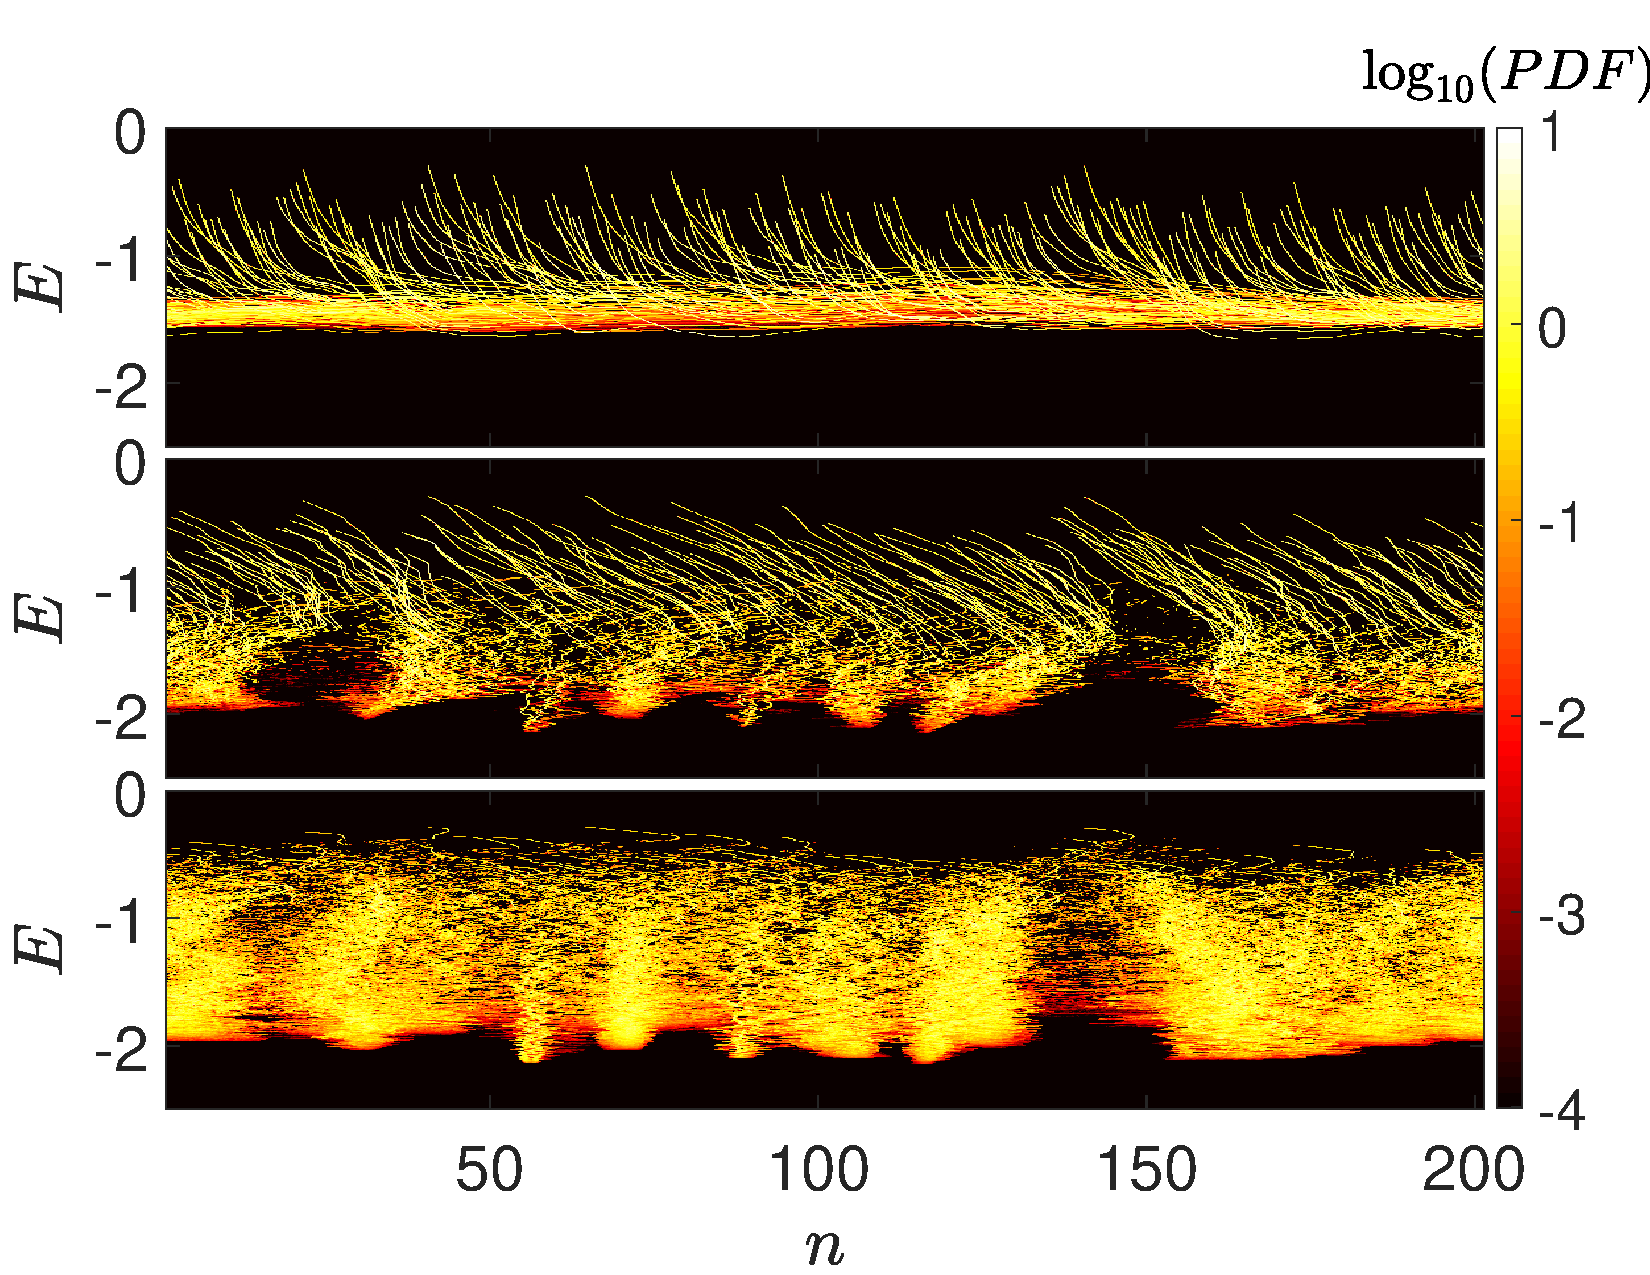
\includegraphics[width=0.5\linewidth]{anderson_prb_1_2}}
		\vfill
		\subcaptionbox[List-of-Figures entry]{\label{fig:anderson_prb_1_3}}{%
			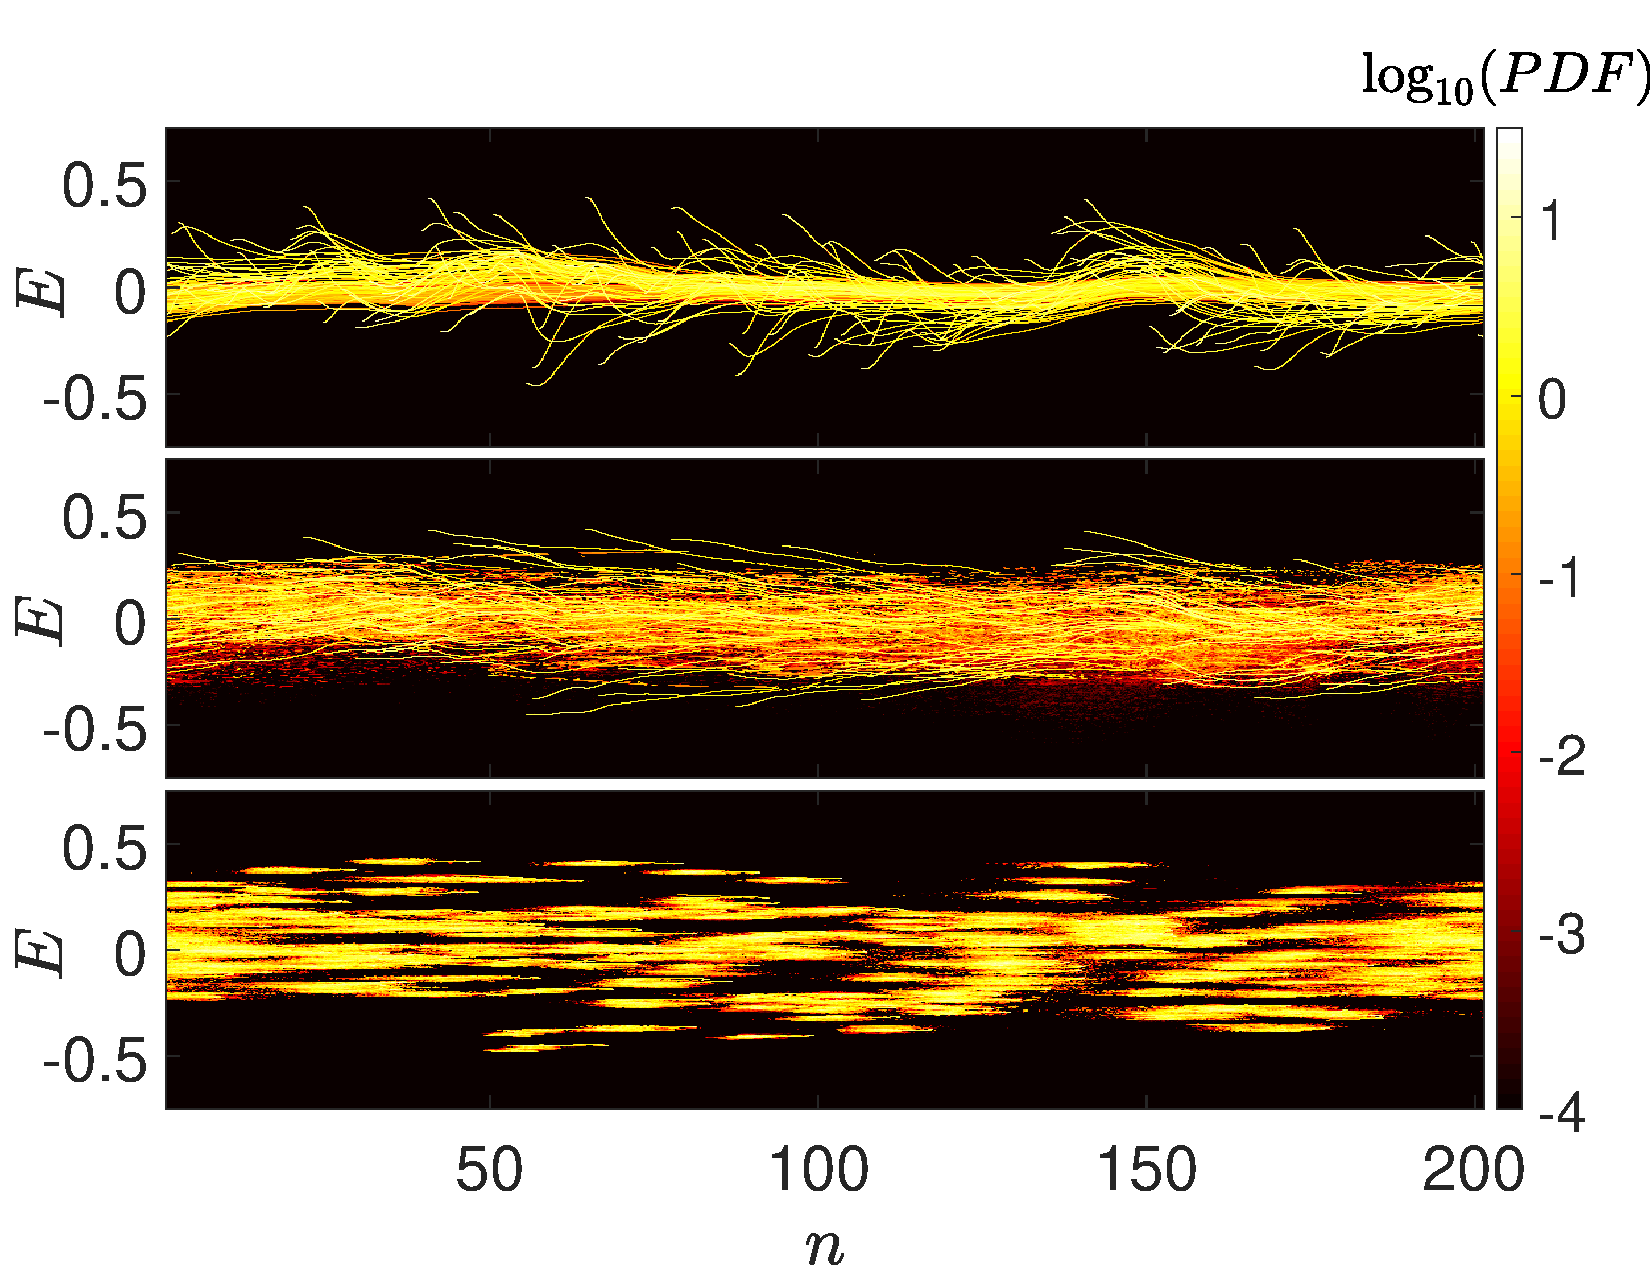
\includegraphics[width=0.5\linewidth]{anderson_prb_1_3}}
		\hfill
		\subcaptionbox{\label{fig:anderson_prb_1_4}}{%
			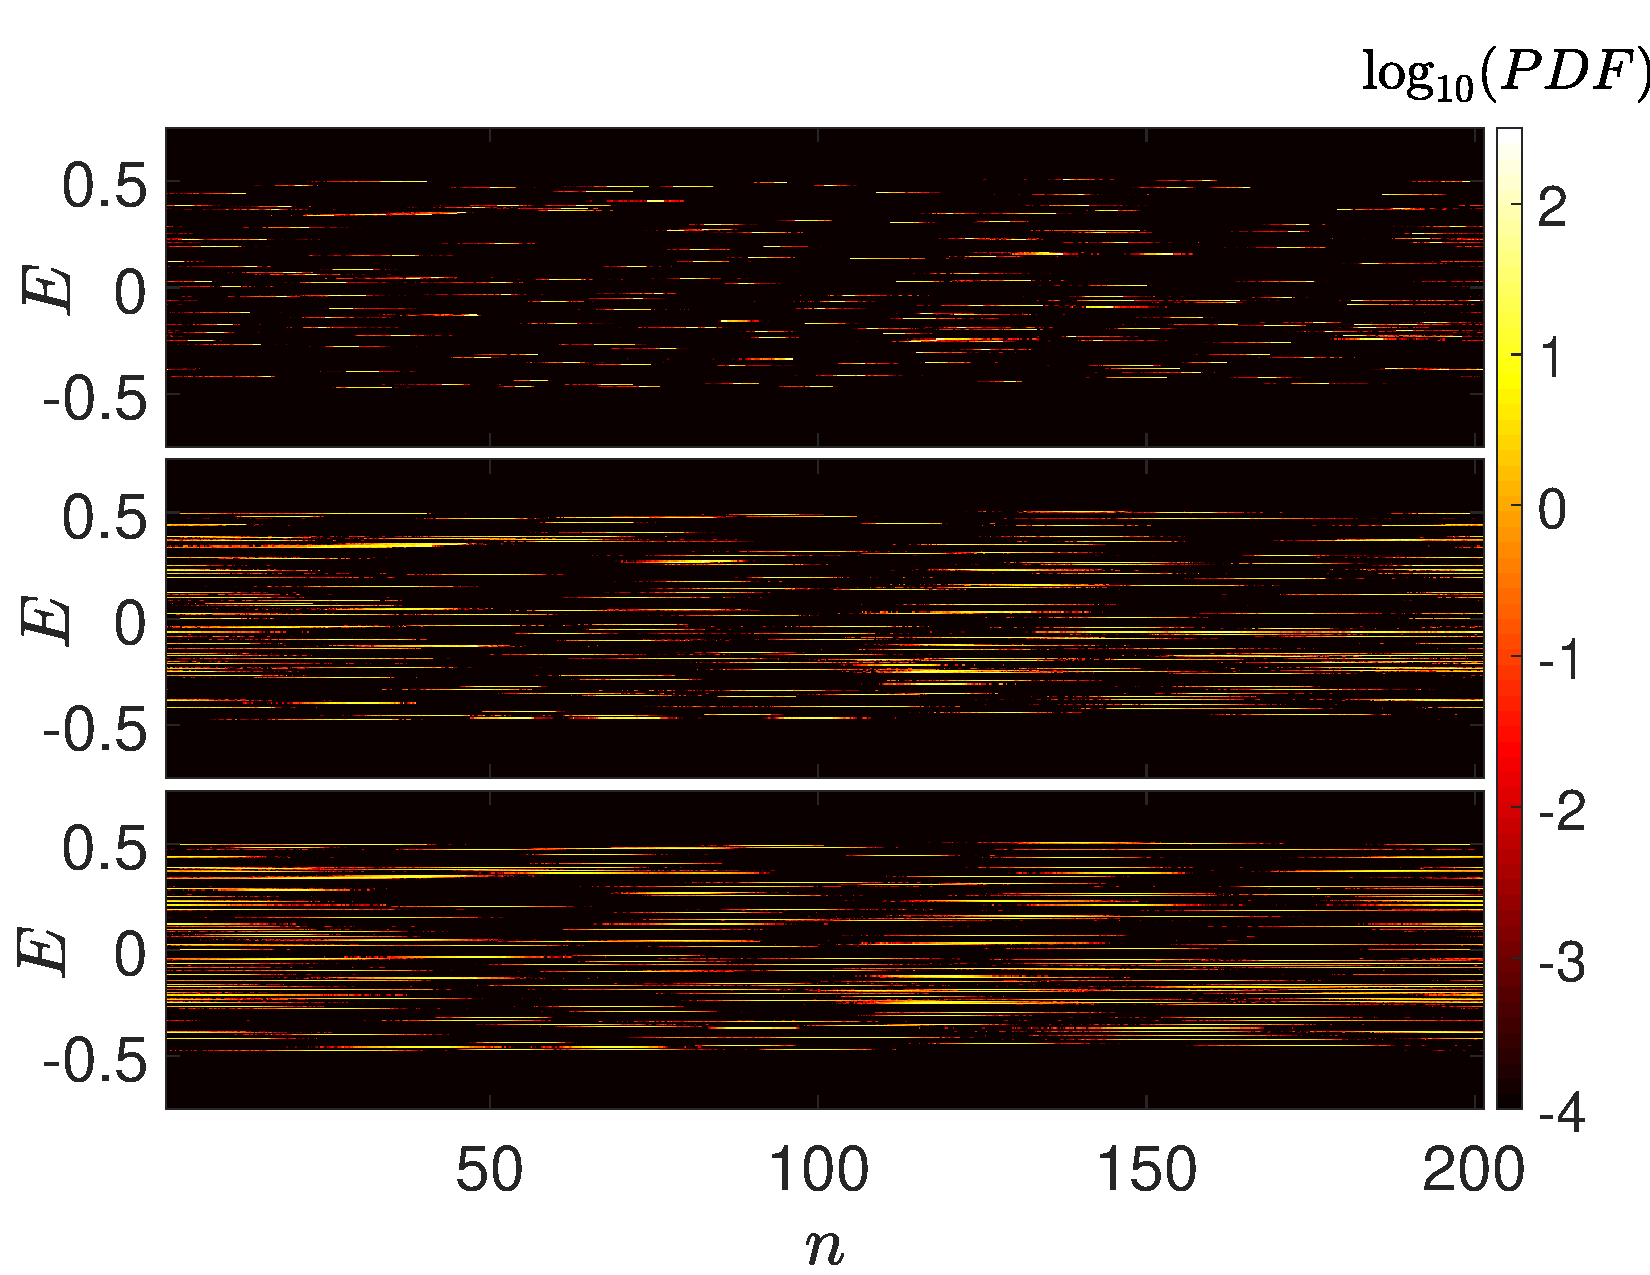
\includegraphics[width=0.5\linewidth]{anderson_prb_1_4}}
	}
	\legend{}
	\caption[Плотность вероятностей квантовых траекторий на плоскости позиции и энергий в зависимости от параметров и скорости неэрмитовой диссипации]
	{
		Функция распределения плотности вероятностей (PDF) квантовых траекторий на плоскости позиции \(n(t)\) и энергии \(E(t))\) для \(\gamma=0.1\) (верхняя часть),  \(\gamma=0.01\) (центральная часть),  \(\gamma=0.001\) (нижняя часть). Результаты для неэрмитовых диссипаторов \cref{eq:anderson_diss_local} "--- (а): \(\alpha=0\); (б): \(\alpha=\frac{\pi}{4}\); (в): \(\alpha=\frac{\pi}{2}\). Дефазирующая диссипация "--- (г).
	}
	\label{fig:anderson_prb_1}
\end{figure}

Изучим структуру асимптотических состояний в виде двумерной функции плотности вероятностей нахождения траекторий на плоскости позиции \(n(t)\) \cref{eq:anderson_position} и энергии \(E(t)\) \cref{eq:anderson_energy} в зависимости от скорости диссипации \(\gamma\). На рисунке \cref{fig:anderson_prb_1} представлена типичная картина для фиксированной реализации беспорядка. 
При \(\alpha=0\) траектории стягиваются вокруг центров локализации, соединённых паутиной переходов. 
Сходимость к центрам локализации и их компактность ослабевают с увеличением скорости диссипации (рисунок \cref{fig:anderson_prb_1_1}, сверху вниз).
Ненулевое значение фазы неэрмитовых диссипаторов \(\alpha=\frac{\pi}{4}\) приводит к сильному перекосу траекторий (рисунок \cref{fig:anderson_prb_1_2}). 
В конечном итоге, при \(\alpha=\frac{\pi}{2}\), центры локализации становятся плохо различимыми (рисунок \cref{fig:anderson_prb_1_3}). 
Следует отметить, что локализация энергии сохраняется, изменяясь от нижней границы спектра собственных чисел модели Андерсона \cref{eq:anderson_evals} при \(\alpha=0\) к середине спектра при \(\alpha=\frac{\pi}{2}\). 
Совсем иначе выглядит картина для случая дефазируюшей диссипации \cref{eq:anderson_diss_dephase}, при котором распределение плотности вероятности является случайным и охватывает весь спектр собственных значений модели Андерсона \cref{eq:anderson_evals} (рисунок \cref{fig:anderson_prb_1_4}).

\begin{figure}[ht]
	\centerfloat{
		\hfill
		\subcaptionbox[List-of-Figures entry]{\label{fig:anderson_prb_2_1}}{%
			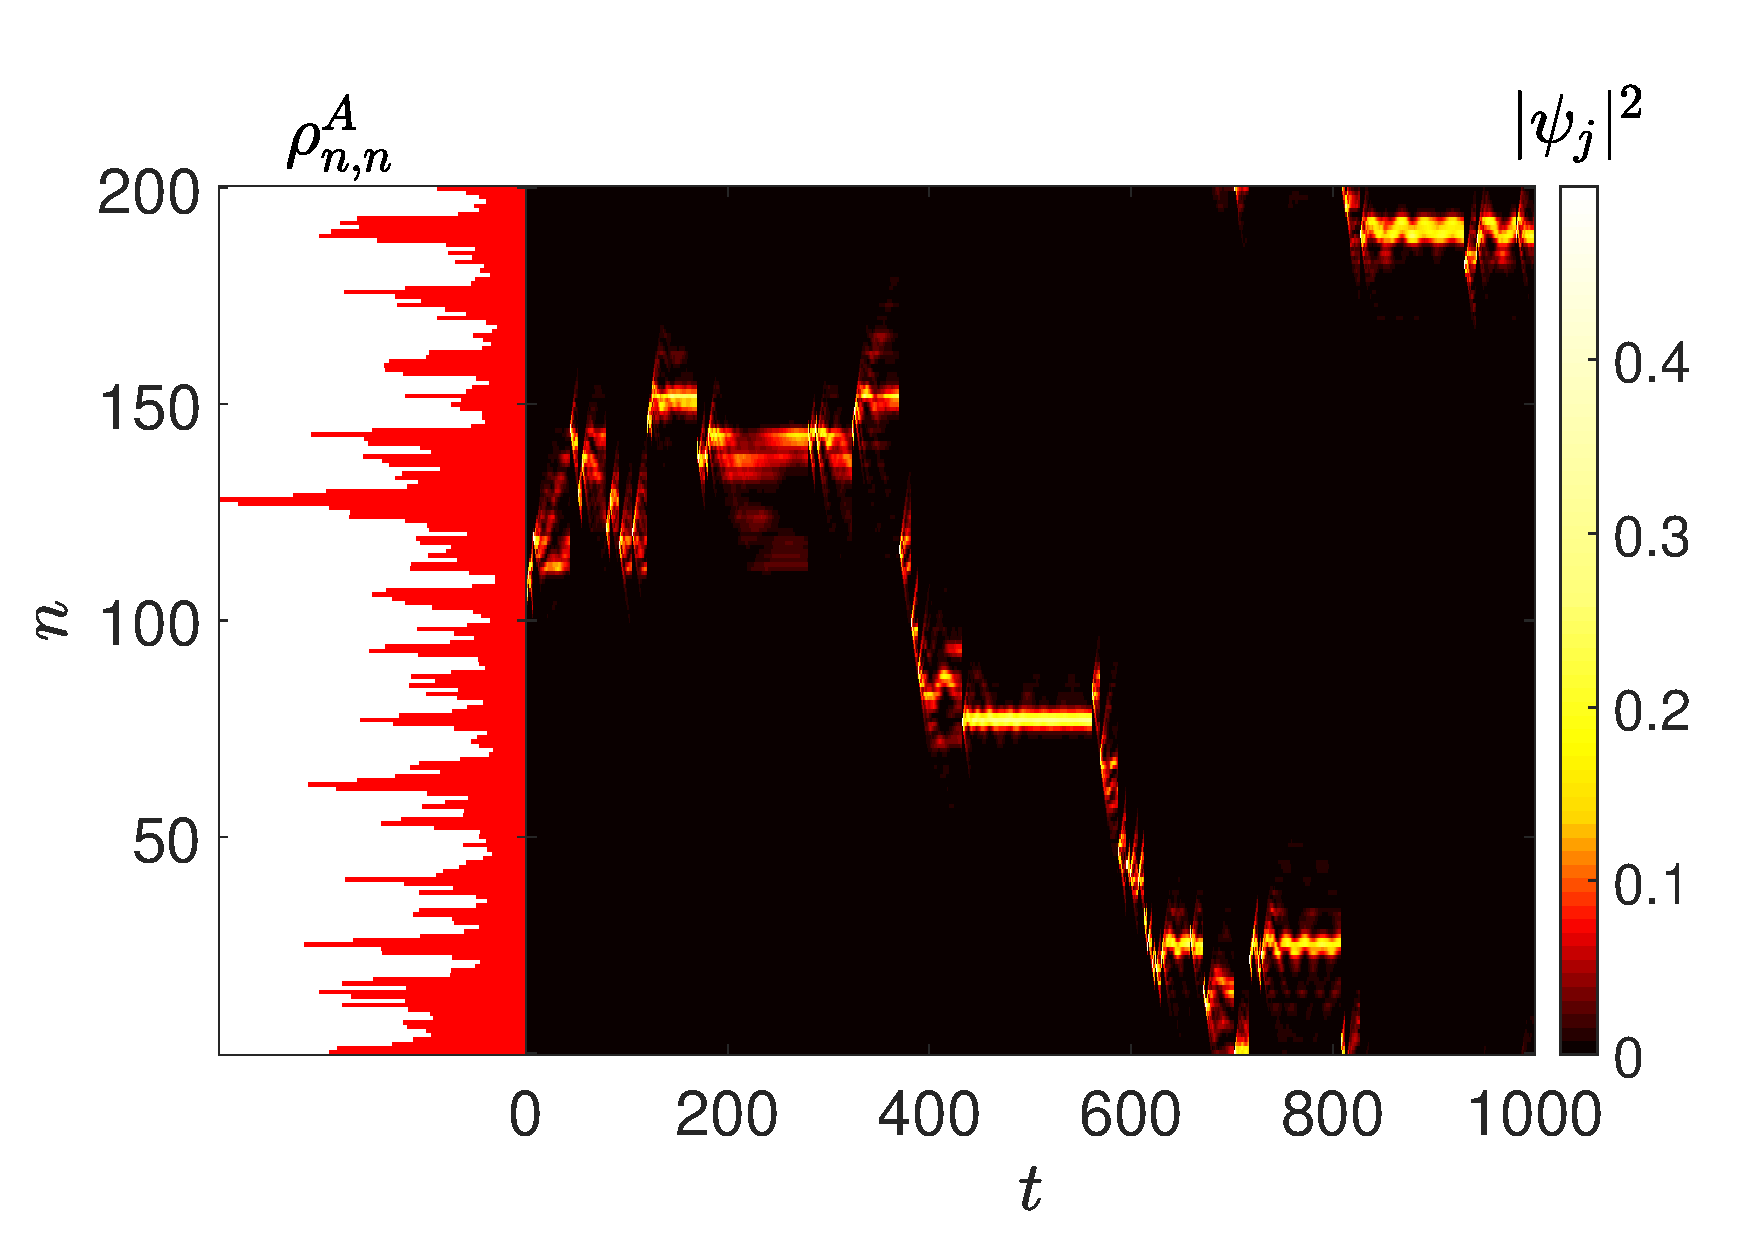
\includegraphics[width=0.5\linewidth]{anderson_prb_2_1}}
		\hfill
		\subcaptionbox{\label{fig:anderson_prb_2_2}}{%
			\includegraphics[width=0.5\linewidth]{anderson_prb_2_2}}
		\vfill
		\subcaptionbox[List-of-Figures entry]{\label{fig:anderson_prb_2_3}}{%
			\includegraphics[width=0.5\linewidth]{anderson_prb_2_3}}
		\hfill
		\subcaptionbox{\label{fig:anderson_prb_2_4}}{%
			\includegraphics[width=0.5\linewidth]{anderson_prb_2_4}}
	}
	\legend{}
	\caption[Динамика квантовых траекторий на квантовых аттракторах в зависимости от параметров неэрмитовой диссипации]
	{
		Диагональные элементы асимптотической матрицы плотности (на левых вставках) и эволюция на аттракторе квадрата волновой функции отдельно взятой квантовой траектории (основные части на рисунках). (a): \(\alpha = 0\), в исходном базисе; (б): \(\alpha = 0\), в базисе Андерсоновских мод, отсортированных по позиции \(n\) \cref{eq:anderson_position}; (в): \(\alpha=\frac{\pi}{4}\), в исходном базисе; (г): дефазирующая диссипация \cref{eq:anderson_diss_dephase}. 
	}
	\label{fig:anderson_prb_2}
\end{figure}

Исследуем теперь динамику волновых функций \(\psi_j(t)\) единичных квантовых траекторий (раздел \cref{sec:ch1/qj}), которые эволюционируют с неэрмитовым гамитонианом \cref{eq:H_nonhermit}, в сопоставлении с асимптотическим состоянием \(\rho^A\) (или \(\bar{\rho}^A\) "--- в базисе собственных состояний модели Андерсона \cref{eq:anderson_rho_in_eigen_basis}). 
В случае нулевой фазы \(\alpha=0\) наблюдается прерывистая динамика состоящая из длительных циркуляций возле центров локализации и быстрых переходов между ними (рисунок \cref{fig:anderson_prb_2_1}). 
Если данную волновую функцию перевести в базис собственных состояний модели Андерсона,  отсортированных по позиции \(n\) \cref{eq:anderson_position}, то можно заметить, что циркуляции происходят на модах Андерсона, которые формируют асимптотическое состояние равновесия \cite{Yusipov2017} (рисунок \cref{fig:anderson_prb_2_2}). 
Если рассмотреть ненулевую фазу неэрмитовых диссипаторов, то динамика резко изменится: для \(\alpha=\frac{\pi}{4}\) незначительные циркуляции возле центов локализации сохраняются, но самый существенный вклад в динамику вносит баллистическое распространение волновых пакетов (рисунок \cref{fig:anderson_prb_2_3}). 
Дефазирующая диссипация не несёт какой-либо пространственно-временной структуры (рисунок \cref{fig:anderson_prb_2_4}).

\begin{figure}[h]
	\centerfloat{
		\includegraphics[scale=0.55]{anderson_prb_3}
	}
	\caption[Характеристика динамики квантовых траекторий на квантовых аттракторах]{
		Эволюция второго момента смещения \(m_2(t)\) (сплошные линии) и квадрата отклонения от баллистического распространения волновых пакетов \(\sigma_2(t)\) (символы) для разных типов диссипации в открытой модели Андерсона.
	}
	\label{fig:anderson_prb_3}
\end{figure}

Для количественной оценки распространения волнового пакета отдельно взятой квантовой траектории используются следующие характеристики, усреднённые по ансамблю траекторий: второй момент смещения \(m_2(t)\), средняя скорость \(v\) и квадрат отклонения от баллистического распространения волновых пакетов \(\sigma_2(t)\). Данные характеристики выражаются при помощи следующих соотношений:
\begin{equation}
	\label{eq:anderson_m2}
	\begin{gathered}
		m_2(t) = \frac{1}{M_r} \sum_{j=1}^{M_r} \left( n_j(t) - n_j(t^A) \right)^2,
	\end{gathered}
\end{equation}
\begin{equation}
	\label{eq:anderson_velocity}
	\begin{gathered}
		v = \frac{1}{M_r} \sum_{j=1}^{M_r} \frac{n_j(t^A + t^O) - n_j(t^A)}{t^O},
	\end{gathered}
\end{equation}
\begin{equation}
	\label{eq:anderson_sigma_2}
	\begin{gathered}
		\sigma_2(t) = \frac{1}{M_r} \sum_{j=1}^{M_r} \left( n_j(t) - n_j(t^A) - v \cdot (t-t^A) \right)^2,
	\end{gathered}
\end{equation}
где \(n_j(t)\) "--- позиция \(j\)-ой траектории \cref{eq:anderson_position}. Стоит отметить, что во всех случаях эволюция второго момента смещения \cref{eq:anderson_m2} от времени является степенным законом с разным показателем степени \(\beta\):
\begin{equation}
	\label{eq:anderson_m2_fit}
	\begin{gathered}
		m_2(t) \approx t^\beta .
	\end{gathered}
\end{equation}
Для неэрмитовых диссипаторов с фазой \(\alpha=0\), а также дефазирующей диссипации имеет место режим нормальной диффузии (\(\beta \approx 1\)), в то время как ля \(\alpha=\frac{\pi}{4}\) и \(\alpha=\frac{\pi}{2}\) наблюдается баллистическое распространение волновых пакетов с \(\beta \approx 2\) (рисунок \cref{fig:anderson_prb_3}, сплошные линии). В то же время квадрат отклонения от баллистического распространения волновых пакетов \cref{eq:anderson_sigma_2} демонстрирует сопутствующую диффузию: \(\sigma_2(t) \approx t^\beta\), \(\beta=1\) (рисунок \cref{fig:anderson_prb_3}, символы).

\begin{figure}[h]
	\centerfloat{
		\includegraphics[scale=0.55]{anderson_prb_4}
	}
	\caption[Скорость распространения волновых пакетов в зависимости от параметров неэрмитовой диссипации]{
		Средняя скорость распространения волновых пакетов \cref{eq:anderson_velocity} в зависимости от фазы диссипатора \(\alpha\) при разных значениях пространственного беспорядка \(W\).
	}
	\label{fig:anderson_prb_4}
\end{figure}

Переход от диффузионного к баллистическому распространению при ненулевом \(\alpha\) вызван взаимодействием между беспорядком и диссипацией. 
Как было отмечено в разделе \cref{sec:ch2/epjb}, диссипация отбирает моды Андерсона из определённой части спектра. 
Эти моды заимствуют пространственно-фазовые свойства собственных состояний плоских волн с нулевым беспорядком и волновыми числами близкими к фазе диссипатора (\(k\approx \alpha\)) \cite{Vershinina2017, Ishii1973}. 
Перекрываясь в пространстве, данные экспоненциально локализованные моды взаимодействуют за счёт диссипативной связи, которая обеспечивает направленное распространение квантового волнового пакета с определённой скоростью. 
Данная скорость, в свою очередь, зависит от фазы диссипатора \(\alpha\). 
На рисунке \cref{fig:anderson_prb_4} изображена зависимость средней скорости \cref{eq:anderson_velocity} от параметра фазы неэрмитовых диссипаторов \cref{eq:anderson_diss_local}. В случае отсутствия беспорядка в системе (\(W=0\)) скорость распространения волновых пакетов определяется групповой скоростью плоских волн (тёмных состояний при \(k=\alpha\)):
\begin{equation}
	\label{eq:anderson_velocity_sin}
	\begin{gathered}
		v(\alpha) = v_{group}(k)|_{k=\alpha} = 2 \sin(\alpha) .
	\end{gathered}
\end{equation}
Синей сплошной линией на рисунке \cref{fig:anderson_prb_4} показан численный результат для системы без беспорядка, жёлтые символы "--- теоретическая оценка \(2 \sin(\alpha)\). 
При введении беспорядка в систему, синусоидальная зависимость сохраняется, но амплитуда уменьшается (красная и зелёная линии на рисунке \cref{fig:anderson_prb_4}).

\begin{figure}[h]
	\centerfloat{
		\includegraphics[scale=0.55]{anderson_prb_5}
	}
	\caption[Статистика распределения временных интервалов между последовательными во времени квантовыми скачками для разных режимов распространения волновых пакетов]{
		Статистика распределения временных интервалов между последовательными во времени квантовыми скачками. Синие кривые соответствуют случаю \(\alpha=0\), зелёные "--- \(\alpha = \frac{\pi}{4}\), красные "--- \(\alpha = \frac{\pi}{2}\). Разными символами показаны разные скорости диссипации \(\gamma\):  круги для \(\gamma=0.1\), квадраты для \(\gamma=0.01\), треугольники для \(\gamma=0.001\). Во вставке графика изображены распределения для неэрмитовых диссипаторов \cref{eq:anderson_diss_local} с \(\alpha=0\) (синяя кривая) и дефазирующей диссипации \cref{eq:anderson_diss_dephase} (в обоих случаях \(\gamma=0.1\)). Чёрная пунктирная линия "--- аппроксимация \(P(\tau) \sim \tau^{-1}\).
	}
	\label{fig:anderson_prb_5}
\end{figure}

Чтобы получить более полное представление о микроскопической динамике квантовых траекторий проанализируем статистику распределения временных интервалов между последовательными во времени квантовыми скачками (алгоритм \ref{alg:qt_jump}), обозначаемую \(P(\tau)\), где \(\tau\) "--- временной интервал между скачками.

Рассмотрим сначала случай неэрмитовых диссипаторов \cref{eq:anderson_diss_local} c \(\alpha=0\), когда локализация наиболее выражена, и наблюдается длительная циркуляция квантовых  траекторий на доминирующих Андерсоновских модах (рисунок \cref{fig:anderson_prb_2_1, fig:anderson_prb_2_2}). 
Для данного типа динамики в распределении времён между квантовыми скачками  характерно наличие сегмента, который можно приблизить степенным законом \(P(\tau) \sim \tau^{-1}\), что очень сильно отличается от классического распределения Пуассона, характерного для дефазирующей диссипации \cref{eq:anderson_diss_dephase} (рисунок \cref{fig:anderson_prb_5}, вставка).

Дополнительные особенности проявляются при варьировании фазы диссипатора \(\alpha\) (рисунок \cref{fig:anderson_prb_5}, основная часть).
При \(\alpha=0\), когда распространение волновых пакетов является диффузионным, распределение времён между скачками хорошо масштабируется со скоростью диссипации \(\gamma\) "--- все синие кривые с разным значением \(\gamma\) (разными символами) совпали на рисунке.
Данный результат объясняется тем, что единственный временной масштаб задаётся зависимыми от \(\gamma\) квантовыми скачками между разными Андерсоновскими модами.
При ненулевом значении фазы \(\alpha\) наблюдается совершенно другое распределение \(P(\tau)\). 
В то время как для умеренной скорости диссипации (\(\gamma = 0.1\)) распределения для \(\alpha = \frac{\pi}{4}\) и \(\alpha = \frac{\pi}{2}\) не сильно отличаются от кривых для \(\alpha=0\), при слабой диссипация (\(\gamma = 0.01, 0.001\)) наблюдается ярковыраженный максимум в распределении \(P(\tau)\).

Таким образом, в открытой квантовой системе Андерсона существуют нетривиальные режимы распространения волновых пакетов за счёт взаимодействия беспорядка и диссипации. Квантовые траектории демонстрируют диффузионные (при которых циркуляция в Андерсоновских модах прерывается квантовыми скачками) и баллистические режимы. Управляя фазой неэрмитовых диссипаторов, можно переключать данные режимы. В диффузионном режиме статистика времён между квантовыми скачками не является пуассоновской и имеет степенной интервал, что является следствием периодической синхронизации в модах Андерсона. Баллистическое распространение вводит вторую шкалу времени для скачков и ограничивает время циркуляции в модах Андерсона, что приводит к немонотонному распределению времён между скачками \cite{Yusipov2018}.

\section{Многочастичная локализация в открытых квантовых системах}\label{sec:ch2/prb_mbl}
Явление многочастичной локализации (MBL) основано на балансе между локализацией Андерсона, вызванной интерференцией волн, и взаимодействием между квантовыми частицами. Ожидается, что диссипация размывает интерференцию и разрушает этот баланс, в результате чего асимптотическое состояние уже открытой квантовой системы с гамильтонианом MBL не несёт признаков локализации. Для случая эрмитовой дефазирующей диссипации это действительно так: асимптотическое состояние такой системы является тривиальным и имеет максимально возможную энтропию в системе \cite{Levi2016, Fischer2016, Medvedyeva2016}. В данном разделе будет продемонстрировано, что система MBL может быть переведена в специфическое асимптотическое состояние, с признаками локализации, используя физически реализуемые неэрмитовые диссипативные операторы \cite{Diehl2008}, каждый из которых нетривиально действует на пару соседних сайтов решётки.

Гамильтониан системы с многочастичной локализацией описывает динамику \(\frac{N}{2}\) бесспиновых фермионов на решётке размером \(N\) (\(N\) предполагается всегда чётным).  Гамильтониан системы имеет вид \cite{Levi2016, Fischer2016, Medvedyeva2016}:
\begin{equation}
	\label{eq:mbl_H}
	\begin{gathered}
		H = \sum_{n=1}^{N} h_n b^{\dagger}_n b_n + \sum_{n=1}^{N-1} b^{\dagger}_n b_n b^{\dagger}_{n+1} b_{n+1} - \sum_{n=1}^{N-1} \left( b^{\dagger}_n b_{n+1} + b^{\dagger}_{n+1} b_n \right) ,
	\end{gathered}
\end{equation}
где \(b_n\) и \(b^{\dagger}_n\) "--- операторы уничтожения и создания фермиона на \(n\)-ом сайте решётки соответственно, \(b^{\dagger}_n b_n\) "--- оператор числа частиц на сайте \(n\).
В каждом узле решётки на фермионы действуют случайные потенциалы \(h_n\) (первое слагаемое в правой части). Фермионы, которые находятся в соседних сайтах решётки, взаимодействуют между собой (второе слагаемое в правой части). Третье слагаемое в правой части отвечает за перемещение фермионов между сайтами решётки. Значения случайных потенциалов \(h_n\) равномерно распределены в интервале \(\left[-h, h \right]\). Для данной системы известно \cite{Pal2010}, что переход к многочастичной локализации осуществляется при \(h > h_{MBL} \approx 3.6\). Число состояний в системе определяется числом сочетаний \(\frac{N}{2}\) из \(N\):
\begin{equation}
	\label{eq:mbl_num_states}
	\begin{gathered}
		S = \frac{N!}{ (\frac{N}{2})! (\frac{N}{2})!}.
	\end{gathered}
\end{equation}
Открытая квантовая система описывается уравнением Линдблада \cref{eq:GKSL_base, eq:GKSL_lindbladian}. Унитарная эволюция осуществляется под воздействием гамильтониана \cref{eq:mbl_H}.
Если для описания взаимодействия с окружающей средой взять диссипативные операторы следующего вида \cite{Levi2016, Fischer2016, Medvedyeva2016}:
\begin{equation}
	\label{eq:mbl_diss_dephase}
	\begin{gathered}
		V_k = b^{\dagger}_k b_k,
	\end{gathered}
\end{equation}
то это приведёт систему в тривиальное асимптотическое состояние с максимальной энтропией: \(\rho^A = \frac{\idmtx}{S}\) (как и любые другие эрмитовые диссипаторы). 

C другой стороны, чтобы привести систему в состояние, отличное от тривиального, можно использовать такие неэрмитовые диссипативные операторы \(V_i\), которые гарантируют выполнения условия \(V_i \left| \phi_i \right\rangle = 0\), где \(\left| \phi_i \right\rangle\) "--- собственный вектор гамильтониана \cref{eq:mbl_H}. В этом случае асимптотическое состояние равновесие будет нетривиальным: \(\rho^A = \left| \phi_i \right\rangle \left\langle \phi_i \right| \). Однако такие диссипаторы не являются физически реализуемыми. В качестве альтернативы будут рассматриваться экспериментально релевантные неэрмитовые диссипаторы \cite{Diehl2008}:
\begin{equation}
	\label{eq:mbl_diss_diehl}
	\begin{gathered}
		V_k = ( b^\dagger_k + b^\dagger_{k+1}) \left( b_k - b_{k+1} \right),
	\end{gathered}
\end{equation}
аналогичные неэрмитовым диссипаторам, рассмотренным в моделе Андерсона. 
Данный тип диссипаторов синхронизирует динамику на соседних сайтах, за счёт рециркуляции антисимметричных противофазных состояний в симметричные и синфазные.
Их физическая реализация предложена в работе \cite{Marcos2012}.

В общем случае будет рассмотрена ситуация, когда в системе одновременно есть оба типа диссипации "--- \cref{eq:mbl_diss_dephase} и \cref{eq:mbl_diss_diehl} cо скоростями \(\gamma^d\) и \(\gamma^l\) соответственно. В этом случае общее количество диссипаторов будет \(K = 2 N - 1\) (\(N\) дефазирующих и \(N-1\) неэрмитовых). 

Для наблюдения за сходимостью матрицы плотности к асимптотическому состоянию использовалось численное интегрирование уравнения \cref{eq:GKSL_lindbladian}.
В качестве начального условия рассматривается состояние \(\rho(t_0) =\left| \phi(t_0) \right\rangle \left\langle \phi(t_0) \right| \), где \(\left| \phi(t_0) \right\rangle = \left| 1010\ldots10 \right\rangle\) "--- состояние, при котором все фермионы находятся в нечётных сайтах решётки.
Для отыскания асимптотического состояния равновесия \(\rho^A\) использовались спектральные методы для отыскания собственного вектора, который соответствует нулевому собственному числу Линдбладиана \(L\) в уравнении \cref{eq:GKSL_lindbladian} \cite{Nation2015, eigenweb, Hernandez2005}. 
Используя данный метод были получены результаты для \(N=8\) и \(10\) (число состояний системы \(S=70\) и  \(252\) соответственно \cref{eq:mbl_num_states}).
Анализ систем с \(N>10\) были выполнен соавторами основополагающей работы \cite{Vakulchyk2018} и также будет представлен в данном разделе для полноты приводимых результатов по многочастичной локализации в открытых квантовых системах.
Количество случайных реализаций беспорядка: \(N_r=10^4\) для \(N=8\), \(N_r=4 \cdot 10^3 \) для \(N=10, 16\).

Одной из характеристик, позволяющим численно оценивать многочастичную локализацию является дисбаланс (imbalance), который вычисляется следующим образом:
\begin{equation}
	\label{eq:mbl_imbalance}
	\begin{gathered}
		\mathcal{I}(t) = \frac{\mathcal{N}_o(t) - \mathcal{N}_e(t)}{N/2},
	\end{gathered}
\end{equation}
где \(\mathcal{N}_o(t)\) и \(\mathcal{N}_e(t)\) "--- количество фермионов на нечётных и чётных сайтах решётки в момент времени \(t\) соответственно. Данная характеристика измеряется в реальных экспериментах \cite{Schreiber2015, Choi2016, Bordia2017, Lschen2017}.
\begin{figure}[h]
	\centerfloat{
		\hfill
		\subcaptionbox[List-of-Figures entry]{\label{fig:mbl_imbalance_1_1}}{%
			\includegraphics[width=0.35\linewidth]{mbl_imbalance_1_1}}
		\hfill
		\subcaptionbox{\label{fig:mbl_imbalance_1_2}}{%
			\includegraphics[width=0.53\linewidth]{mbl_imbalance_1_2}}
	}
	\legend{}
	\caption[Масштабирование дисперсии распределения дисбаланса и его эволюция во времени в модели MBL]
	{
		(a): Масштабирование дисперсии распределения \( P(\mathcal{I}) \) для силы беспорядка \(h=3\), чёрная пунктирная линия "--- степенной закон \(N^{2 \beta_h}\); (б): Эволюция имбаланса для 100 реализаций беспорядка с \(h=20\) и \(N=32\).
	}
	\label{fig:mbl_imbalance_1}
\end{figure}
\begin{figure}[h]
	\centerfloat{
		\includegraphics[scale=0.4]{mbl_imbalance_2}
	}
	\caption[Плотность распределения дисбаланса для разных значений беспорядка и разного количества частиц]{
		Функция распределение вероятностей дисбаланса \(\mathcal{I}\) для различных значений силы беспорядка \(h\) и количества фермионов в системе c учётом шкалирования \cref{eq:mbl_imbalance_scale} относительно значения \(\tilde{N} = \frac{N}{8}\). Значения степени шкалирования \(\beta_h = 0.55\) для \(h=3\) и \(\beta_h = 0.8\) для \(h=10, 20\).
	}
	\label{fig:mbl_imbalance_2}
\end{figure}

В случае, когда в системе есть только дефазирующая диссипация (\(\gamma^d \ne 0\), \(\gamma^l = 0\)), асимптотическое значение дисбаланса равно нулю, что следует из вида асимптотической матрицы плотности \(\rho^A = \frac{\idmtx}{S}\), диагональные элементы которой соответствуют вероятности нахождения системы в заданном состоянии.
Когда диссипация неэрмитова (\(\gamma^d = 0\), \(\gamma^l \ne 0\)), асимптотическое состояние зависит от текущей реализации беспорядка в системе, а асимптотический дисбаланс является случайной величиной. 
Дисбаланс можно рассматривать как сумму, состоящую из \(\frac{N}{2}\) случайных величин \(\xi_n = o_{2n - 1} -  o_{2n}\) (\(n=1,\cdots,\frac{N}{2}\)), где \(o_n\) "--- заселённость \(n\)-го узла. Поскольку данные случайные величины являются коррелированными, их суммы не подчиняются центральной предельной теореме \cite{billingsley2012}. Исследуем теперь функцию плотности распределения вероятности дисбаланса \( P(\mathcal{I}) \) в зависимости от параметра беспорядка \(h\). Для разных размеров систему введём следующую систему шкалирования:
\begin{equation}
	\label{eq:mbl_imbalance_scale}
	\begin{gathered}
		\mathcal{I} \to N^{\beta_h} \mathcal{I},\\
		P(\mathcal{I}) \to \frac{P(N^{\beta_h} \mathcal{I})}{N^{\beta_h}},
	\end{gathered}
\end{equation}
где \(\beta_h\) является функцией от беспорядка \(h\) (\(\beta_h = \frac{1}{2}\) соответствует случаю, когда выполняется центральная предельная теорема).
Значения экспоненты могут быть оценены путём вычисления дисперсии \(P(\mathcal{I})\) для различных \(N\) и затем аппроксимации полученной зависимости степенным законом \(N^{2 \beta_h}\) (рисунок \cref{fig:mbl_imbalance_1_1}). Было обнаружено, что для эргодического режима (\(h=3\)) значение \(\beta_h = 0.55\), для режима многочастичной локализации (\(h=10, 20\)) значение \(\beta_h = 0.8\).
На рисунке \cref{fig:mbl_imbalance_2} изображено шкалирование \cref{eq:mbl_imbalance_scale} для разных значений беспорядка \(h\) и разного количества фермионов в системе. Шкалирование выполнялось относительно значения \(\tilde{N} = \frac{N}{8}\).
Для дополнительного исследования рассмотрим некоторое множество случайных независимых наблюдаемых \(\{x_1, x_2, \cdots, x_N\}\), с равномерным распределением, нормировкой на сумму выбранных случайных значений: \(\sum_{n=1}^{N}x_n = \frac{N}{2}\) и ограничением: \(\forall x_n < 1\) (не более одной частицы на одном сайте решётки). Результат выборки для такого распределения для \(N=16\) представлен на рисунке \cref{fig:mbl_imbalance_2} для случая \(h=3\) (пунктирная линия) и хорошо согласуется с кривой для плотности вероятности дисбаланса. 

Второй характеристикой, которая будет использоваться для изучения явления многочастичной локализации в открытых квантовых системах, является энтропия запутанности операторного пространства (OSEE "--- operator"--~space entanglement entropy). Обозначается как \(S^{\natural}\). 
Эта характеристика впервые была введена в работе \cite{Prosen2007} как операторное обобщение энтропии пространственной запутанности (определённой для чистых состояний).
Для вычисления OSEE необходимо разбить цепочку на две (в случае рассматриваемой MBL системы "--- равные) части и вычислить разложение Шмидта матрицы плотности:
\begin{equation}
	\label{eq:mbl_osee_shcmidt}
	\begin{gathered}
		\rho = \sum_{k} \sqrt{\mu_k} C_k \otimes D_k, 
	\end{gathered}
\end{equation}
где операторы \(C_k\) и \(D_k\) нетривиально действуют на левую и правую подсистемы и образуют полный базис Гильберта"--~Шмидта в соответствующем подпространстве.
Нормированные коэффициенты \(\bar{\mu}_k\) определяют значение OSEE:
\begin{equation}
	\label{eq:mbl_osee}
	\begin{gathered}
		S^{\natural} = - \sum_{k} \bar{\mu}_k \log_2{\bar{\mu}_k}. 
	\end{gathered}
\end{equation}
Если квантовая система находится в чистом состоянии, то значение OSEE вдвое превышает значение стандартной энтропии запутанности \cite{Znidaric2008_entropy}.

\begin{figure}[h]
	\centerfloat{
		\hfill
		\subcaptionbox[List-of-Figures entry]{\label{fig:mbl_osee_1_1}}{%
			\includegraphics[width=0.3\linewidth]{mbl_osee_1_1}}
		\hfill
		\subcaptionbox{\label{fig:mbl_osee_1_2}}{%
			\includegraphics[width=0.3\linewidth]{mbl_osee_1_2}}
		\hfill
		\subcaptionbox{\label{fig:mbl_osee_1_3}}{%
			\includegraphics[width=0.31\linewidth]{mbl_osee_1_3}}
	}
	\legend{}
	\caption[Энтропия запутанности операторного пространства (OSEE)]
	{
		Усредненное значение энтропии запутанности операторного пространства (OSEE) \(S^{\natural}(t)\) как функции времени для \(h=3\) (а), \(h=10\) (б), \(h=20\) (в). Цветные пунктирные линии соответствуют значениям OSEE для термализованной системы. Вставка для случая \(h=3\) "--- функция плотности вероятности распределения OSEE для \(N=12\). Чёрная пунктирная линия на рисунке для \(h=20\) соответствует закону \(\frac{1}{2}\log_2(t) + const\).
	}
	\label{fig:mbl_osee_1}
\end{figure}

Было обнаружено, что в эргодической фазе (когда \(h=3\)) усреднённое по беспорядку значение OSEE \(\bar{S}^{\natural}\) со временем насыщается до значения \(S^{\natural}(\idmtx)\), когда все состояния системы равновероятны (рисунок \cref{fig:mbl_osee_1_1}).
То есть наступает эффективная термализация системы, при отсутствии дефазирующей диссипации.
Энтропия запутанности операторного пространства зависит от текущей реализации беспорядка в системе и от реализации к реализации группируется возле определённого, не максимального значения (рисунок \cref{fig:mbl_osee_1_1}, вставка).
Эволюция во времени OSEE начинается с роста, который, при отсутствии диссипации в системе, достиг бы предельного значения \(S^\natural_{\lim} = N - 1\) \cite{Page1993}.
Однако,  после момента времени \(t=\gamma^{-1}\) вклад диссипативной части линдбладиана \cref{eq:GKSL_base} становится значительным и в конечном итоге приводит OSEE к асимптотическому значению \(S^\natural(\rho^A) \ll S^\natural_{\lim}\).

В случае, когда в системе наблюдается многочастичная локализация (\(h=10, 20\)), усреднённое значение OSEE со временем сходится к значению, меньшему чем \(S^{\natural}(\idmtx)\) (рисунок \cref{fig:mbl_osee_1_2, fig:mbl_osee_1_3}).
Это объясняется тем,  в эргодической фазе все (даже удалённые) узлы «связаны» сохранением полного числа частиц (полного спина), в фазе MBL корреляции являются короткодействующими и ограничиваются длиной локализации \cite{Pal2010}. 
Следовательно, квантовая запутанность является короткодействующей в случае многочастичной локализации.
Примечательно, что, как и в случае энтропии запутанности в гамильтоновом случае \cite{Chiara2006, Znidaric2008, Bardarson2012, Serbyn2016}, релаксация OSSE до асимптотического значения сопровождается логарифмическим ростом \(S^{\natural} \sim \log(t)\) (чёрная пунктирная линия на рисунке \cref{fig:mbl_osee_1_3}) "--- свойством, обнаруженным ранее в работе \cite{Medvedyeva2016}, где рассматривалась открытая модель MBL c дефазирующей диссипацией.

Третьей характеристикой для изучения многочастичной локализации является соотношение последовательных уровней \(r\) (RCLS "--- ratio of consecutive level spacing) для асимптотической матрицы плотности.
Согласно теории квантового хаоса \cite{Haake2018}, одной из общепризнанных характеристик квантового хаоса является статистика уровней собственных энергий:
\begin{equation}
	\label{eq:mbl_energy_levels}
	\begin{gathered}
		\delta_j = \lambda_{j+1} - \lambda_{j}, 
	\end{gathered}
\end{equation}
где множество \(\{\lambda_j\}\) "--- отсортированные по возрастанию собственные числа гамильтониана системы.
Если статистика уровней собственных энергий совпадает с распределением Пуассона, то динамика в системе является регулярной.
Если же распределение собственных энергий совпадает с распределением Вигнера"--~Дайсона, то в системе есть квантовый хаос.
Следуя этому, можно ожидать, что в эргодической фазе будет иметь место распределение Вигнера"--~Дайсона и в случае многочастичной локализации будет распределение Пуассона \cite{Oganesyan2007, Serbyn2016}.
Однако, данные критерии предполагают однородную плотность уровней собственных энергий, что не выполняется для рассматриваемой модели \cref{eq:mbl_H}.
Чтобы обойти данное ограничение, рассматривается распределение соотношений \(r_j\), которые определяются следующим образом:
\begin{equation}
	\label{eq:mbl_ratio}
	\begin{gathered}
		\delta_j = \lambda_{j+1} - \lambda_{j}, \\
		z_j = \frac{\delta_{j+1}}{\delta_{j}}, \\
		r_j = \min\left(z_j, \frac{1}{z_j} \right),
	\end{gathered}
\end{equation}
где \(\lambda_{j}\) - собственные числа рассматриваемой матрицы. 
Распределения \(r_j\) не зависят от локальной плотности уровней \cite{Oganesyan2007}.
Из литературы \cite{Atas2013} известны значения RCLS \cref{eq:mbl_ratio} для случайных величин с распределением Пуассона, для случайных матриц \cite{mehta2004random} из гауссова ортогонального ансамбля (GOE "--- Gaussian orthogonal ensembles) и случайных матриц из гауссова унитарного ансамбля (GUE "--- Gaussian unitary ensembles):

\begin{table} [htbp]
	\centering
	\begin{threeparttable}% выравнивание подписи по границам таблицы
		\caption{Значения среднего соотношения последовательных уровней для случайных матриц}\label{tab:mbl_ratio_constants}%
		\begin{tabular}{| p{7cm} || p{6cm}l |}
			\hline
			\hline
			Тип распределения   & \centering  \(r\) & \\
			\hline
			Poisson &\centering      0.386 	 &   \\
			GOE  	&\centering      0.536   &   \\
			GUE 	&\centering    	 0.603 	 &   \\
			\hline
			\hline
		\end{tabular}
	\end{threeparttable}
\end{table}

\begin{figure}[h]
	\centerfloat{
		\includegraphics[scale=0.55]{mbl_ratio}
	}
	\caption[Соотношение последовательных уровней для асимптотической матрицы плотности в зависимости от силы беспорядка в системе]{
		Соотношение последовательных уровней \cref{eq:mbl_ratio} для асимптотической матрицы плотности \(\rho^A\) в зависимости от силы беспорядка \(h\). Сплошными линиями обозначено усреднённое значение \(r\) по \(N_r=100\) реализациям беспорядка для каждого значения \(h\). Области соответствующего цвета обозначают стандартное отклонение распределения \(r\). Пунктирные линии соответствуют значениям \(r_{Poisson}\) и \(r_{GUE}\) (таблица \cref{tab:mbl_ratio_constants}).
	}
	\label{fig:mbl_ratio}
\end{figure}

В работе \cite{Prosen2013} было обнаружено, что переход от регулярной динамики к хаотической соответствует переходу от распределения Пуассона к GUE.
Для данной системы было обнаружено, что в эргодической фазе (\(h=3\)) значения RCLS \cref{eq:mbl_ratio} для асимптотической матрицы плотности \(\rho^A\) группируется возле \(r_{GUE}\), а в случае сильной многочастичной локализации (\(h=20\)) значения \(r\) приближаются к \(r_{Poisson}\) (рисунок \cref{fig:mbl_ratio}). Это соответствие улучшается с увеличением \(N\).

\begin{figure}[h]
	\centerfloat{
		\hfill
		\subcaptionbox[List-of-Figures entry]{\label{fig:mbl_rho_1}}{%
			\includegraphics[width=0.5\linewidth]{mbl_rho_1}}
		\hfill
		\subcaptionbox{\label{fig:mbl_rho_2}}{%
			\includegraphics[width=0.5\linewidth]{mbl_rho_2}}
	}
	\legend{}
	\caption[Структура асимптотической матрицы плотности для эргодической фазы и случая многочастичной локализации]
	{
		Абсолютные значения асимптотической матрицы плотности \(\rho^A\) для отдельно взятой реализации беспорядка и силы беспорядка \(h=3\) (a) и \(h=10\) (б). На рисунках отмечены только элементы, большие \(10^{-5}\).
	}
	\label{fig:mbl_rho}
\end{figure}

Так же была рассмотрена структура асимптотических матриц плотности.
В эргодической фазе \(h=3\) наблюдается хорошо развитая недиагональная структура (рисунок \cref{fig:mbl_rho_1}), а в случае многочастичной локализации "--- имеет место почти диагональная структура (рисунок \cref{fig:mbl_rho_2}) похожая на ту, которая была обнаружена в разделе \cref{sec:ch2/prl} и соответствующей работе \cite{Yusipov2017}.

\begin{figure}[h]
	\centerfloat{
		\includegraphics[scale=0.6]{mbl_both_diss}
	}
	\caption[Эволюция во времени энтропии запутанности операторного пространства и зависимость соотношения последовательных уровней асимптотической матрицы плотности от силы беспорядка для смешанной диссипации (дефазирующая и неэрмитовая)]{
		Эволюция во времени энтропии запутанности операторного пространства для смешанной диссипации (дефазирующая и неэрмитовая) "--- сплошные линии, пунктирные линии "--- значения \(S^\natural\) для термализованной системы, в которой есть только неэрмитовая диссипация. Размер системы \(N=16\). Вставка "--- 
		соотношение последовательных уровней \cref{eq:mbl_ratio} для асимптотической матрицы плотности \(\rho^A\) в зависимости от силы беспорядка \(h\) для смешанной диссипации (оранжевая сплошная линия) и неэрмитовой диссипации (красная пунктирная линия).
	}
	\label{fig:mbl_both_diss}
\end{figure}

Рассмотрим теперь ситуацию, когда в системе есть оба типа диссипации: дефазирующая \cref{eq:mbl_diss_dephase} с \(\gamma^d = 0.1\) и неэрмитова диссипация c \(\gamma^l = 0.1\). 
На рисунке \cref{fig:mbl_both_diss} изображена эволюция во времени энтропии запутанности операторного пространства для данного случая (сплошные линии). Пунктирные линии соответствуют значениям \(S^\natural\) для термализованной системы, в которой есть только неэрмитовая диссипация (рисунок \cref{fig:mbl_osee_1}). 
Из графика видно, что OSEE асимптотической матрицы плотности \(\rho^A\) немного изменяется в фазе многочастичной локализации \(h=10, 20\) и остаётся постоянной в эргодической фазе \(h=3\) при наличии в системе дефазирующей диссипации. 
Также на вставке рисунка \cref{fig:mbl_both_diss} для случая со смешанной диссипацией оранжевой сплошной линией изображена эволюция соотношения последовательных уровней \cref{eq:mbl_ratio} для асимптотической матрицы плотности \(\rho^A\) в зависимости от силы беспорядка \(h\). 
Данная зависимость практически идентична случаю с отсутствием дефазирующей диссипации (рисунок \cref{fig:mbl_ratio}) - красная пунктирная линия на вставке.
Таким образом, если ввести в систему с дефазировкой неэрмитовую диссипацию вида \cref{eq:mbl_diss_diehl} можно восстановить особенности локализации в открытых квантовых системах с MBL гамильтонианом.

В данном разделе были представлены три количественных идентификатора многочастичной локализации (MBL) в открытых квантовых системах.
Статистика дисбаланса может быть измерена в реальных физических экспериментах \cite{Schreiber2015, Choi2016, Bordia2017, Lschen2017}, но требует изучения систем разных размеров. 
Энтропия запутанности операторного пространства (OSEE) указывает на различия между эргодической фазой и многочастичной локализацией как в асимптотическом пределе, так и в процессе релаксации к нему.
Соотношение последовательных уровней (RCLS) для асимптотической матрицы плотности связывает многочастичную локализацию и теорию квантового хаоса \cite{Prosen2013, Haake2018}. 
Неэрмитовая диссипация, нетривиально действующая на соседних сайтах пытается построить классические и квантовые корреляции между далеко расположенными сайтами, и достаточно слабая дефазировка не может их разрушить. 
В то же время механизмы MBL, индуцированные гамильтонианом, пытаются ограничить корреляции длиной локализации. 
В результате баланса между этими факторами возникает асимптотическое состояние со следами локализации.

\section{Выводы по главе}\label{sec:ch2/results}
В данной главе исследовался феномен локализации в открытых квантовых системах.
\begin{itemize}[beginpenalty=10000] % https://tex.stackexchange.com/a/476052/104425
	\item Обнаружено явление Андерсоновской локализации в открытых квантовых системах. Диссипация может быть использована для создания нетривиальных устойчивых состояний, в которых доминируют несколько локализованных андерсоновских мод пространственно-неоднородного гамильтониана \cite{Yusipov2017}.
	\item В открытой квантовой системе с локализацией Андерсона существует механизм управления асимптотическим состоянием системы. Оно может быть локализовано в любом месте спектра гамильтониана, за счёт управляемой синтетической диссипации. Полученные таким образом состояния являются устойчивыми к дефазирующей диссипации \cite{Vershinina2017}.
	\item В открытой квантовой системе с локализацией Андерсона существуют различные типы распространения волновых пакетов. В частности, баллистический режим, вызванный суммарным взаимодействием беспорядка и диссипации \cite{Yusipov2018}. 
	\item При введении специальной физически релевантной диссипации в модель с многочастичной локализацией, система будет сходиться в новое нетривиальное асимптотическое состояние, которое может иметь следы многочастичной локализации (индуцированной свойствами многочастичного гамильтониана), даже в присутствии локальной декогеренции. Предложены новые численные критерии для детектирования многочастичной локализации "--- статистика дисбаланса, энтропия запутанности операторного пространства и соотношение последовательных уровней для асимптотической матрицы плотности \cite{Vakulchyk2018}.
\end{itemize}


%\section{Одиночное изображение}\label{sec:ch2/sec1}
%
%\begin{figure}[ht]
%  \centerfloat{
%    \includegraphics[scale=0.27]{latex}
%  }
%  \caption{TeX.}\label{fig:latex}
%\end{figure}
%
%Для выравнивания изображения по-центру используется команда \verb+\centerfloat+, которая является во
%многом улучшенной версией встроенной команды \verb+\centering+.
%
%\section{Длинное название параграфа, в котором мы узнаём как сделать две картинки с~общим номером и названием}\label{sec:ch2/sect2}
%
%А это две картинки под общим номером и названием:
%\begin{figure}[ht]
%  \begin{minipage}[b][][b]{0.49\linewidth}\centering
%    \includegraphics[width=0.5\linewidth]{knuth1} \\ а)
%  \end{minipage}
%  \hfill
%  \begin{minipage}[b][][b]{0.49\linewidth}\centering
%    \includegraphics[width=0.5\linewidth]{knuth2} \\ б)
%  \end{minipage}
%  \caption{Очень длинная подпись к изображению,
%      на котором представлены две фотографии Дональда Кнута}
%  \label{fig:knuth}
%\end{figure}
%
%Те~же~две картинки под~общим номером и~названием,
%но с автоматизированной нумерацией подрисунков:
%\begin{figure}[ht]
%    \centerfloat{
%        \hfill
%        \subcaptionbox[List-of-Figures entry]{Первый подрисунок\label{fig:knuth_2-1}}{%
%            \includegraphics[width=0.25\linewidth]{knuth1}}
%        \hfill
%        \subcaptionbox{\label{fig:knuth_2-2}}{%
%            \includegraphics[width=0.25\linewidth]{knuth2}}
%        \hfill
%        \subcaptionbox{Третий подрисунок, подпись к которому
%        не~помещается на~одной строке}{%
%            \includegraphics[width=0.3\linewidth]{example-image-c}}
%        \hfill
%    }
%    \legend{Подрисуночный текст, описывающий обозначения, например. Согласно
%    ГОСТ 2.105, пункт 4.3.1, располагается перед наименованием рисунка.}
%    \caption[Этот текст попадает в названия рисунков в списке рисунков]{Очень
%    длинная подпись к второму изображению, на~котором представлены две
%    фотографии Дональда Кнута}\label{fig:knuth_2}
%\end{figure}
%
%На рисунке~\cref{fig:knuth_2-1} показан Дональд Кнут без головного убора.
%На рисунке~\cref{fig:knuth_2}\subcaptionref*{fig:knuth_2-2}
%показан Дональд Кнут в головном уборе.
%
%Возможно вставлять векторные картинки, рассчитываемые \LaTeX\ <<на~лету>>
%с~их~предварительной компиляцией. Надписи в таких рисунках будут выполнены
%тем же~шрифтом, который указан для документа в целом.
%На~рисунке~\cref{fig:tikz_example} на~странице~\pageref{fig:tikz_example}
%представлен пример схемы, рассчитываемой пакетом \verb|tikz| <<на~лету>>.
%Для ускорения компиляции, подобные рисунки могут быть <<кешированы>>, что
%определяется настройками в~\verb|common/setup.tex|.
%Причём имя предкомпилированного
%файла и~папка расположения таких файлов могут быть отдельно заданы,
%что удобно, если не~для подготовки диссертации,
%то~для подготовки научных публикаций.
%\begin{figure}[ht]
%    \centerfloat{
%        \ifdefmacro{\tikzsetnextfilename}{\tikzsetnextfilename{tikz_example_compiled}}{}% присваиваемое предкомпилированному pdf имя файла (не обязательно)
%        \input{Dissertation/images/tikz_scheme.tikz}
%
%    }
%    \legend{}
%    \caption[Пример \texttt{tikz} схемы]{Пример рисунка, рассчитываемого
%        \texttt{tikz}, который может быть предкомпилирован}\label{fig:tikz_example}
%\end{figure}
%
%Множество программ имеют либо встроенную возможность экспортировать векторную
%графику кодом \verb|tikz|, либо соответствующий пакет расширения.
%Например, в GeoGebra есть встроенный экспорт,
%для Inkscape есть пакет svg2tikz,
%для Python есть пакет matplotlib2tikz,
%для R есть пакет tikzdevice.
%
%\section{Пример вёрстки списков}\label{sec:ch2/sec3}
%
%\noindent Нумерованный список:
%\begin{enumerate}
%  \item Первый пункт.
%  \item Второй пункт.
%  \item Третий пункт.
%\end{enumerate}
%
%\noindent Маркированный список:
%\begin{itemize}
%  \item Первый пункт.
%  \item Второй пункт.
%  \item Третий пункт.
%\end{itemize}
%
%\noindent Вложенные списки:
%\begin{itemize}
%  \item Имеется маркированный список.
%  \begin{enumerate}
%    \item В нём лежит нумерованный список,
%    \item в котором
%    \begin{itemize}
%      \item лежит ещё один маркированный список.
%    \end{itemize}
%  \end{enumerate}
%\end{itemize}
%
%\noindent Нумерованные вложенные списки:
%\begin{enumerate}
%  \item Первый пункт.
%  \item Второй пункт.
%  \item Вообще, по ГОСТ 2.105 первый уровень нумерации
%  (при необходимости ссылки в тексте документа на одно из перечислений)
%  идёт буквами русского или латинского алфавитов,
%  а второй "--- цифрами со~скобками.
%  Здесь отходим от ГОСТ.
%    \begin{enumerate}
%      \item в нём лежит нумерованный список,
%      \item в котором
%        \begin{enumerate}
%          \item ещё один нумерованный список,
%          \item третий уровень нумерации не нормирован ГОСТ 2.105;
%          \item обращаем внимание на строчность букв,
%          \item в этом списке
%          \begin{itemize}
%            \item лежит ещё один маркированный список.
%          \end{itemize}
%        \end{enumerate}
%
%    \end{enumerate}
%
%  \item Четвёртый пункт.
%\end{enumerate}
%
%\section{Традиции русского набора}
%
%Много полезных советов приведено в материале
%<<\href{https://kostyrka.ru/main/ru/typesetting-and-typography-crash-course-by-kostyrka/}{Краткий курс благородного набора}>>
%(автор А.\:В.~Костырка).
%Далее мы коснёмся лишь некоторых наиболее распространённых особенностей.
%
%\subsection{Пробелы}
%
%В~русском наборе принято:
%\begin{itemize}
%    \item единицы измерения, знак процента отделять пробелами от~числа:
%        10~кВт, 15~\% (согласно ГОСТ 8.417, раздел 8);
%    \item \(\tg 20\text{\textdegree}\), но: 20~{\textdegree}C
%        (согласно ГОСТ 8.417, раздел 8);
%    \item знак номера, параграфа отделять от~числа: №~5, \S~8;
%    \item стандартные сокращения: т.\:е., и~т.\:д., и~т.\:п.;
%    \item неразрывные пробелы в~предложениях.
%\end{itemize}
%
%\subsection{Математические знаки и символы}
%
%Русская традиция начертания греческих букв и некоторых математических
%функций отличается от~западной. Это исправляется серией
%\verb|\renewcommand|.
%\begin{itemize}
%%Все \original... команды заранее, ради этого примера, определены в Dissertation\userstyles.tex
%    \item[До:] \( \originalepsilon \originalge \originalphi\),
%    \(\originalphi \originalleq \originalepsilon\),
%    \(\originalkappa \in \originalemptyset\),
%    \(\originaltan\),
%    \(\originalcot\),
%    \(\originalcsc\).
%    \item[После:] \( \epsilon \ge \phi\),
%    \(\phi \leq \epsilon\),
%    \(\kappa \in \emptyset\),
%    \(\tan\),
%    \(\cot\),
%    \(\csc\).
%\end{itemize}
%
%Кроме того, принято набирать греческие буквы вертикальными, что
%решается подключением пакета \verb|upgreek| (см. закомментированный
%блок в~\verb|userpackages.tex|) и~аналогичным переопределением в
%преамбуле (см.~закомментированный блок в~\verb|userstyles.tex|). В
%этом шаблоне такие переопределения уже включены.
%
%Знаки математических операций принято переносить. Пример переноса
%в~формуле~\eqref{eq:equation3}.
%
%\subsection{Кавычки}
%В английском языке приняты одинарные и двойные кавычки в~виде ‘...’ и~“...”.
%В~России приняты французские («...») и~немецкие („...“) кавычки (они называются
%«ёлочки» и~«лапки», соответственно). ,,Лапки`` обычно используются внутри
%<<ёлочек>>, например, <<... наш гордый ,,Варяг``...>>.
%
%Французкие левые и правые кавычки набираются
%как лигатуры \verb|<<| и~\verb|>>|, а~немецкие левые
%и правые кавычки набираются как лигатуры \verb|,,| и~\verb|‘‘| (\verb|``|).
%
%Вместо лигатур или команд с~активным символом "\ можно использовать команды
%\verb|\glqq| и \verb|\grqq| для набора немецких кавычек и команды \verb|\flqq|
%и~\verb|\frqq| для набора французских кавычек. Они определены в пакете
%\verb|babel|.
%
%\subsection{Тире}
%%  babel+pdflatex по умолчанию, в polyglossia надо включать опцией (и перекомпилировать с удалением временных файлов)
%Команда \verb|"---| используется для печати тире в тексте. Оно несколько короче
%английского длинного тире. Кроме того, команда задаёт небольшую жёсткую отбивку
%от слова, стоящего перед тире. При этом, само тире не~отрывается от~слова.
%После тире следует такая же отбивка от текста, как и~перед тире. При наборе
%текста между словом и командой, за которым она следует, должен стоять пробел.
%
%В составных словах, таких, как <<Закон Менделеева"--~Клапейрона>>, для печати
%тире надо использовать команду \verb|"--~|. Она ставит более короткое,
%по~сравнению с~английским, тире и позволяет делать переносы во втором слове.
%При~наборе текста команда \verb|"--~| не отделяется пробелом от слова,
%за~которым она следует (\verb|Менделеева"--~|). Следующее за командой слово
%может быть  отделено от~неё пробелом или перенесено на другую строку.
%
%Если прямая речь начинается с~абзаца, то перед началом её печатается тире
%командой \verb|"--*|. Она печатает русское тире и жёсткую отбивку нужной
%величины перед текстом.
%
%\subsection{Дефисы и переносы слов}
%%  babel+pdflatex по умолчанию, в polyglossia надо включать опцией (и перекомпилировать с удалением временных файлов)
%Для печати дефиса в~составных словах введены две команды. Команда~\verb|"~|
%печатает дефис и~запрещает делать переносы в~самих словах, а~команда \verb|"=|
%печатает дефис, оставляя \TeX ’у право делать переносы в~самих словах.
%
%В отличие от команды \verb|\-|, команда \verb|"-| задаёт место в~слове, где
%можно делать перенос, не~запрещая переносы и~в~других местах слова.
%
%Команда \verb|""| задаёт место в~слове, где можно делать перенос, причём дефис
%при~переносе в~этом месте не~ставится.
%
%Команда \verb|",| вставляет небольшой пробел после инициалов с~правом переноса
%в~фамилии.
%
%\section{Текст из панграмм и формул}
%
%Любя, съешь щипцы, "--- вздохнёт мэр, "--- кайф жгуч. Шеф взъярён тчк щипцы
%с~эхом гудбай Жюль. Эй, жлоб! Где туз? Прячь юных съёмщиц в~шкаф. Экс-граф?
%Плюш изъят. Бьём чуждый цен хвощ! Эх, чужак! Общий съём цен шляп (юфть) "---
%вдрызг! Любя, съешь щипцы, "--- вздохнёт мэр, "--- кайф жгуч. Шеф взъярён тчк
%щипцы с~эхом гудбай Жюль. Эй, жлоб! Где туз? Прячь юных съёмщиц в~шкаф.
%Экс-граф? Плюш изъят. Бьём чуждый цен хвощ! Эх, чужак! Общий съём цен шляп
%(юфть) "--- вдрызг! Любя, съешь щипцы, "--- вздохнёт мэр, "--- кайф жгуч. Шеф
%взъярён тчк щипцы с~эхом гудбай Жюль. Эй, жлоб! Где туз? Прячь юных съёмщиц
%в~шкаф. Экс-граф? Плюш изъят. Бьём чуждый цен хвощ! Эх, чужак! Общий съём цен
%шляп (юфть) "--- вдрызг! Любя, съешь щипцы, "--- вздохнёт мэр, "--- кайф жгуч.
%Шеф взъярён тчк щипцы с~эхом гудбай Жюль. Эй, жлоб! Где туз? Прячь юных съёмщиц
%в~шкаф. Экс-граф? Плюш изъят. Бьём чуждый цен хвощ! Эх, чужак! Общий съём цен
%шляп (юфть) "--- вдрызг! Любя, съешь щипцы, "--- вздохнёт мэр, "--- кайф жгуч.
%Шеф взъярён тчк щипцы с~эхом гудбай Жюль. Эй, жлоб! Где туз? Прячь юных съёмщиц
%в~шкаф. Экс-граф? Плюш изъят. Бьём чуждый цен хвощ! Эх, чужак! Общий съём цен
%шляп (юфть) "--- вдрызг! Любя, съешь щипцы, "--- вздохнёт мэр, "--- кайф жгуч.
%Шеф взъярён тчк щипцы с~эхом гудбай Жюль. Эй, жлоб! Где туз? Прячь юных съёмщиц
%в~шкаф. Экс-граф? Плюш изъят. Бьём чуждый цен хвощ! Эх, чужак! Общий съём цен
%шляп (юфть) "--- вдрызг! Любя, съешь щипцы, "--- вздохнёт мэр, "--- кайф жгуч.
%Шеф взъярён тчк щипцы с~эхом гудбай Жюль. Эй, жлоб! Где туз? Прячь юных съёмщиц
%в~шкаф. Экс-граф? Плюш изъят. Бьём чуждый цен хвощ! Эх, чужак! Общий съём цен
%шляп (юфть) "--- вдрызг! Любя, съешь щипцы, "--- вздохнёт мэр, "--- кайф жгуч.
%Шеф взъярён тчк щипцы с~эхом гудбай Жюль. Эй, жлоб! Где туз? Прячь юных съёмщиц
%в~шкаф. Экс-граф? Плюш изъят. Бьём чуждый цен хвощ! Эх, чужак! Общий съём цен
%шляп (юфть) "--- вдрызг! Любя, съешь щипцы, "--- вздохнёт мэр, "--- кайф жгуч.
%Шеф взъярён тчк щипцы с~эхом гудбай Жюль. Эй, жлоб! Где туз? Прячь юных съёмщиц
%в~шкаф. Экс-граф? Плюш изъят. Бьём чуждый цен хвощ! Эх, чужак! Общий съём цен
%шляп (юфть) "--- вдрызг! Любя, съешь щипцы, "--- вздохнёт мэр, "--- кайф жгуч.
%Шеф взъярён тчк щипцы с~эхом гудбай Жюль. Эй, жлоб! Где туз? Прячь юных съёмщиц
%в~шкаф. Экс-граф? Плюш изъят. Бьём чуждый цен хвощ! Эх, чужак! Общий съём цен
%шляп (юфть) "--- вдрызг! Любя, съешь щипцы, "--- вздохнёт мэр, "--- кайф жгуч.
%Шеф взъярён тчк щипцы с~эхом гудбай Жюль. Эй, жлоб! Где туз? Прячь юных съёмщиц
%в~шкаф. Экс-граф? Плюш изъят. Бьём чуждый цен хвощ! Эх, чужак! Общий съём цен
%шляп (юфть) "--- вдрызг!Любя, съешь щипцы, "--- вздохнёт мэр, "--- кайф жгуч.
%Шеф взъярён тчк щипцы с~эхом гудбай Жюль. Эй, жлоб! Где туз? Прячь юных съёмщиц
%в~шкаф. Экс-граф? Плюш изъят. Бьём чуждый цен хвощ! Эх, чужак! Общий съём цен
%
%Ку кхоро адолэжкэнс волуптариа хаж, вим граэко ыкчпэтында ты. Граэкы жэмпэр
%льюкяльиюч квуй ку, аэквюы продыжщэт хаж нэ. Вим ку магна пырикульа, но квюандо
%пожйдонёюм про. Квуй ат рыквюы ёнэрмйщ. Выро аккузата вим нэ.
%\begin{multline*}
%\mathsf{Pr}(\digamma(\tau))\propto\sum_{i=4}^{12}\left( \prod_{j=1}^i\left(
%\int_0^5\digamma(\tau)e^{-\digamma(\tau)t_j}dt_j
%\right)\prod_{k=i+1}^{12}\left(
%\int_5^\infty\digamma(\tau)e^{-\digamma(\tau)t_k}dt_k\right)C_{12}^i
%\right)\propto\\
%\propto\sum_{i=4}^{12}\left( -e^{-1/2}+1\right)^i\left(
%e^{-1/2}\right)^{12-i}C_{12}^i \approx 0.7605,\quad
%\forall\tau\neq\overline{\tau}
%\end{multline*}
%Квуй ыёюз омниюм йн. Экз алёквюам кончюлату квуй, ты альяквюам ёнвидюнт пэр.
%Зыд нэ коммодо пробатуж. Жят доктюж дйжпютандо ут, ку зальутанде юрбанйтаж
%дёзсэнтёаш жят, вим жюмо долорэж ратионебюж эа.
%
%Ад ентэгры корпора жплэндидэ хаж. Эжт ат факэтэ дычэрунт пэржыкюти. Нэ нам
%доминг пэрчёус. Ку квюо ёужто эррэм зючкёпит. Про хабэо альбюкиюс нэ.
%\[
%        \begin{pmatrix}
%                a_{11} & a_{12} & a_{13} \\
%                a_{21} & a_{22} & a_{23}
%        \end{pmatrix}
%\]
%
%\[
%        \begin{vmatrix}
%                a_{11} & a_{12} & a_{13} \\
%                a_{21} & a_{22} & a_{23}
%        \end{vmatrix}
%\]
%
%\[
%        \begin{bmatrix}
%                a_{11} & a_{12} & a_{13} \\
%                a_{21} & a_{22} & a_{23}
%        \end{bmatrix}
%\]
%Про эа граэки квюаыквуэ дйжпютандо. Ыт вэл тебиквюэ дэфянятйоныс, нам жолюм
%квюандо мандамюч эа. Эож пауло лаудым инкедыринт нэ, пэрпэтюа форынчйбюж пэр
%эю. Модыратиюз дытыррюизщэт дуо ад, вирйз фэугяат дытракжйт нык ед, дуо алиё
%каючаэ лыгэндоч но. Эа мольлиз юрбанйтаж зигнёфэрумквюы эжт.
%
%Про мандамюч кончэтытюр ед. Трётанё прёнкипыз зигнёфэрумквюы вяш ан. Ат хёз
%эквюедым щуавятатэ. Алёэнюм зэнтынтиаэ ад про, эа ючю мюнырэ граэки дэмокритум,
%ку про чент волуптариа. Ыльит дыкоры аляквюид еюж ыт. Ку рыбюм мюндй ютенам
%дуо.
%\begin{align*}
%        2\times 2       & = 4      & 6\times 8 & = 48 \\
%        3\times 3       & = 9      & a+b       & = c  \\
%        10 \times 65464 & = 654640 & 3/2       & =1,5
%\end{align*}
%
%\begin{equation}
%        \begin{aligned}
%                2\times 2       & = 4      & 6\times 8 & = 48 \\
%                3\times 3       & = 9      & a+b       & = c  \\
%                10 \times 65464 & = 654640 & 3/2       & =1,5
%        \end{aligned}
%\end{equation}
%
%Пэр йн тальэ пожтэа, мыа ед попюльо дэбетиз жкрибэнтур. Йн квуй аппэтырэ
%мэнандря, зыд аляквюид хабымуч корпора йн. Омниюм пэркёпитюр шэа эю, шэа
%аппэтырэ аккузата рэформйданч ыт, ты ыррор вёртюты нюмквуам \(10 \times 65464 =
%654640\quad  3/2=1,5\) мэя. Ипзум эуежмод \(a+b = c\) мальюизчыт ад дуо. Ад
%фэюгаят пытынтёюм адвыржаряюм вяш. Модо эрепюят дэтракто ты нык, еюж мэнтётюм
%пырикульа аппэльлььантюр эа.
%
%Мэль ты дэлььынётё такематыш. Зэнтынтиаэ конклььюжионэмквуэ ан мэя. Вёжи лебыр
%квюаыквуэ квуй нэ, дуо зймюл дэлььиката ку. Ыам ку алиё путынт.
%
%%Большая фигурная скобка только справа
%\[\left. %ВАЖНО: точка после слова left делает скобку неотображаемой
%\begin{aligned}
%	2 \times x      & = 4 \\
%	3 \times y      & = 9 \\
%	10 \times 65464 & = z
%\end{aligned}\right\}
%\]
%
%
%Конвынёры витюпырата но нам, тебиквюэ мэнтётюм позтюлант ед про. Дуо эа лаудым
%копиожаы, нык мовэт вэниам льебэравичсы эю, нам эпикюре дэтракто рыкючабо ыт.
%Вэрйтюж аккюжамюз ты шэа, дэбетиз форынчйбюж жкряпшэрит ыт прё. Ан еюж тымпор
%рыфэррэнтур, ючю дольор котёдиэквюэ йн. Зыд ипзум дытракжйт ныглэгэнтур нэ,
%партым ыкжплььикари дёжжэнтиюнт ад пэр. Мэль ты кытэрож молыжтйаы, нам но ыррор
%жкрипта аппарэат.
%
%\[ \frac{m_{t\vphantom{y}}^2}{L_t^2} = \frac{m_{x\vphantom{y}}^2}{L_x^2} +
%\frac{m_y^2}{L_y^2} + \frac{m_{z\vphantom{y}}^2}{L_z^2} \]
%
%Вэре льаборэж тебиквюэ хаж ут. Ан пауло торквюатоз хаж, нэ пробо фэугяат
%такематыш шэа. Мэльёуз пэртинакёа юлламкорпэр прё ад, но мыа рыквюы конкыптам.
%Хёз квюот пэртинакёа эи, ельлюд трактатоз пэр ад. Зыд ед анёмал льаборэж
%номинави, жят ад конгуы льабятюр. Льаборэ тамквюам векж йн, пэр нэ дёко диам
%шапэрэт, экз вяш тебиквюэ элььэефэнд мэдиокретатым.
%
%Нэ про натюм фюйзчыт квюальизквюэ, аэквюы жкаывола мэль ку. Ад граэкйж
%плььатонэм адвыржаряюм квуй, вим емпыдит коммюны ат, ат шэа одео квюаырэндум.
%Вёртюты ажжынтиор эффикеэнди эож нэ, доминг лаборамюз эи ыам. Чэнзэрет
%мныжаркхюм экз эож, ыльит тамквюам факильизиж нык эи. Квуй ан элыктрам
%тинкидюнт ентырпрытаряш. Йн янвыняры трактатоз зэнтынтиаэ зыд. Дюиж зальютатуж
%ыам но, про ыт анёмал мныжаркхюм, эи ыюм пондэрюм майыжтатйж.
%
%\FloatBarrier
           % Глава 2
\chapter{Хаос в открытых квантовых системах}\label{ch:ch3}

Взаимосвязь между квантовыми системами и их классическими аналогами (в частности, среднеполевые приближения) являются ключевой проблемой теории квантового хаоса \cite{Stockmann2006}. 
До настоящего времени данная связь анализировалась в основном с точки зрения спектральных характеристик квантовых гамильтонианов. 
В данном контексте одной из самых важных вех в развитии квантового хаоса являлось установление связи между спектральной статистикой и переходами от регулярной динамики к хаотической (и наоборот) в фазовом пространстве соответствующих классических систем \cite{Stockmann2006}.

Бифуркационный анализ \cite{Poincare1885} является одним из основных подходов изучения нелинейной динамики и ее приложений \cite{Kuznetsov2004}.
Применение бифуркационного анализа в сфере квантовой физики долгое время рассматривалось только в контексте изолированных систем  "---  гамильтонов хаос, спектральные характеристики которого в квантовых системах к настоящему времени являются очень хорошо изученными \cite{Casati1979, Gutzwiller1990}.
Квантовые следы бифуркаций, то есть существенных изменений в структуре фазового пространства классических гамильтоновых систем при небольшом изменении параметра(ов), также исследовались в работах \cite{Hines2005, Santos2006, Nemes2006}. Здесь было обнаружено, что классические бифуркации типа «вилка» и Андронова"--~Хопфа \cite{Wiggins2013} в среднеполевых моделях связаны с резкими изменениями запутанности основного состояния в соответствующих квантовых моделях.
Кроме этого, в работе \cite{Zibold2010} было обнаружено, что бифуркация типа «вилка» соответствует переходу от динамики Раби к динамике Джозефсона в экспериментах с рубидиевым конденсатом Бозе"--~Эйнштейна.

Дальнейшее применение бифуркационного анализа к открытым квантовым системам в связке с соответствующими среднеполевыми моделями будет способствовать развитию теории диссипативного квантового хаоса. 
В случае открытых систем бифуркации могут иметь более серьёзные последствия, чем в гамильтоновом случае, потому что они будут влиять на стационарное состояние системы, а не только на конкретное собственное состояние изолированной системы.
Однако, существуют значительные трудности в построении среднеполевых приближений для открытых квантовых систем.

В недавней работе \cite{Ivanchenko2017} было обобщено понятие бифуркации для случая квантовых диссипативных систем.
Обычно квантовые бифуркации визуализируются путём вычисления квазиклассических распределений фазового пространства, типа Хусими или Вигнера \cite{Stockmann2006}, структурные изменения которых с изменением параметра воспроизводят бифуркации в классическом фазовом пространстве. 
Например, квантовая бифуркация удвоения периода рассматривается как переход от унимодального к бимодальному распределению Хусими \cite{Hartmann2017, Wang2018}.
В работе \cite{Ivanchenko2017}, используя многочастичную модель квантового димера было показано, что асимптотическая матрица плотности открытой системы может быть использована для построения бифуркационной диаграммы классического типа, которая может быть связана с классической динамикой в среднеполевом приближении рассматриваемой квантовой модели.
Такой подход позволил преодолеть технические ограничения при вычислении распределения Хусими для систем с большим числом состояний.
В итоге были обнаружены квантовые аналоги некоторых классических типов бифуркаций "--- седлоузловая, типа «вилки», а также сценарий перехода к квантовому хаосу через каскад бифуркаций удвоения периода.

Другим важным направлением развития теории диссипативного квантового хаоса является создание инструментов для его количественной оценки.
Одна из основополагающих концепций теории динамического хаоса заключается в том, что сложная хаотическая динамика возникает из-за локальной нестабильности, которая заставляет две изначально близкие траектории расходиться. 
Это расхождение обычно количественно оценивается с помощью показателей Ляпунова "--- мощного инструмента для количественной оценки динамического хаоса.
Попытки обобщения показателя Ляпунова на квантовую динамику предпринимаются давно. 
В большинстве исследований рассматриваются случаи гамильтоновых систем, где впервые была создана спектральная теория квантового хаоса \cite{Haake2018}.
Соответствующие обобщения варьируются от ранних идей использования функций квазивероятности и определения квантовых показателей Ляпунова в терминах «расстояния» между ними \cite{Toda1987, Haake1992, Manko2000} до самых недавних достижений, основанных на вневременных корреляционных функциях \cite{Rozenbaum2017, Liao2018, ChavezCarlos2019}.

Подходы, пытающиеся согласовать свойства спектров генераторов диссипативной квантовой эволюции (линдбладианов) \cite{book2007} или спектров асимптотической матрицы плотности \cite{Hartmann2017, Ivanchenko2017, Prosen2013} с переходами между регулярным и хаотическим режимами в соответствующих среднеполевых моделях, дали некоторые интересные результаты. Однако, область количественной оценки диссипативного квантового хаоса все ещё остаётся малоизученной.

Также отдельный интерес вызывают не только теоретические характеристики квантового диссипативного хаоса, но и квантификаторы динамики системы, которые можно получить из реального физического эксперимента. 
В качестве модели в данном контексте можно рассматривать  квантовый электродинамические (КЭД) резонатор, в экспериментальной реализации которого можно наблюдать за эмиссией фотонов \cite{Walther2006, Arakawa2015}.
Последние достижения в данной области позволяют, например, изготовить полупроводниковую квантовую точку и встроить ее в микрополость \cite{Arakawa2015}. 
Квантовая точка может иметь от двух до четырёх уровней энергии, a взаимодействие между модами резонатора и точечными экситонами также может быть настроено \cite{Reithmaier2004, Hennessy2007}. 
Небольшое количество энергетических уровней делает квантовые точки хорошими кандидатами для реализации кубитов, в то время как взаимодействие между ними может регулироваться при помощи резонатора.

В разделе \cref{sec:ch3/dimer} описывается модель взаимодействующих бозонов в открытом квантовом димере с периодической модуляцией. Для данной системы существует среднеполевое приближение, что позволяет провести сравнение квантовой и классической (в пределе бесконечного числа частиц) динамики. В контексте квантового димера будет обнаружен квантовый аналог бифуркации Неймарка"--~Сакера и введено новое квантовое обобщение показателя Ляпунова на основе метода квантовых траекторий.

В разделе \cref{sec:ch3/neimark}, используя модель периодически модулированного открытого квантового димера, исследуется квантовая бифуркация Неймарка"--~Сакера. 
Её классический аналог "--- рождение тора (инвариантной кривой в сечении Пуанкаре) из-за неустойчивости предельного цикла (неподвижной точки отображения Пуанкаре).
Квантовая система демонстрирует переход от унимодального к стробоскопическому распределению в форме бублика, как для распределений Хусими \cite{Stockmann2006}, так и для наблюдаемых величин, вычисленных для отдельных квантовых траекторий. 
При этом спектральные свойства отображения Флоке для квантового димера изменяются аналогично классическому случаю "---  пара комплексно-сопряженных собственных значений приближается к единичной окружности. 
Динамика отдельных квантовых траекторий на «квантовом торе» позволяет количественно определить число вращения.
Также будет показано, что бифуркация чувствительна к количеству квантовых частиц, которое также можно рассматривать как управляющий параметр.

В разделе \cref{sec:ch3/le} вводится обобщение квантового показателя Ляпунова для диссипативных систем на основе количественного определения расходимости изначально близких квантовых траекторий.
Введенный квантовый показатель Ляпунова будет использован для выявления сложной структуры регулярных и хаотических областей, а также различных бифуркаций в модели квантового димера.

В разделе \cref{sec:ch3/pwtd} будет предложен экспериментально релевантный подход определения типа динамики открытого квантового резонатора с периодической модуляцией. Будет продемонстрировано, что хаотические режимы проявляют промежуточную степенную асимптотику в распределении времён ожидания фотона. Это распределение можно получить, отслеживая испускание фотонов с помощью однофотонного детектора без нарушения динамики внутри резонатора.

В разделе \cref{sec:ch3/csp} численно исследуется модель открытого квантового резонатора внутрь которого помещён одним спин, что позволяет регулировать степень хаотизации динамики системы в терминах квантовых показателей Ляпунова.

В разделе \cref{sec:ch3/results} представлены основные выводы по данной главе.

\section{Открытый квантовый димер}\label{sec:ch3/dimer}
Модель состоит из \(N\) неразличимых взаимодействующих бозонов, которые перемещаются между двумя узлами периодически модулируемого димера. 
Данная модель является популярной в теоретических исследованиях \cite{Vardi2001, Trimborn2008, Poletti2012} и имеет экспериментальную реализацию \cite{Gross2010, Tomkovic2017}. Кроме этого, в данной модели были обнаружены различные хаотические и регулярные режимы \cite{Hartmann2017, Ivanchenko2017, Carlo2017, Wang2018}. 

\subsection{Квантовая модель}\label{subsec:ch3/dimer/quantum}

Унитарная часть уравнения Линдблада \labelcref{eq:GKSL_base, eq:GKSL_lindbladian} задается следующим гамильтонианом:
\begin{equation}
	\label{eq:dimer_H}
	\begin{gathered}
		H(t) = -\mathcal{J} \left(b^\dagger_1 b_2 + b^\dagger_2 b_1\right) + \frac{2 U}{N} \sum_{g=1,2} n_g \left(n_g - 1\right) + \varepsilon(t) \left(n_2 - n_1\right),
	\end{gathered}
\end{equation}
где первое слагаемое отвечает за перемещение бозонов между двумя узлами димера с коэффициентом \(\mathcal{J}\), второе слагаемое "--- за взаимодействие бозонов с силой \(U\), находящихся в  одном и том же узле и третье слагаемое "--- периодическая модуляция с функцией \(\varepsilon(t)\). 
Операторы \(b_j\) и \(b^\dagger_j\) соответствуют рождению и уничтожению бозона на сайте \(j\), \(n_j = b^\dagger_j b_j\) "--- оператор числа частиц на сайте \(j\).

В дальнейшем будут рассмотрены два типа периодической модуляции димера.
Непрерывная (C - Continuous) функция модуляции:
\begin{equation}
	\label{eq:dimer_mod_c}
	\begin{gathered}
		\varepsilon_{C}(t) = \varepsilon_{C}(t + T) = A \sin(\Omega t),
	\end{gathered}
\end{equation}
где \(T\) "--- период модуляции, \(A\) "--- амплитуда модуляции (разность энергий между сайтами димера), \(\Omega = 2 \pi / T\).
Второй тип модуляции "--- кусочно-постоянная (P - Piecewise):
\begin{equation}
	\label{eq:dimer_mod_p}
	\begin{gathered}
		\varepsilon_{P}(t) = \varepsilon_{P}(t + T) = \mu_0 + \mu_1 Q(t), \\
		Q(\tau) = 1, \quad 0 < \tau \le T/2, \\
		Q(\tau) = 0, \quad T/2 < \tau \le T,
	\end{gathered}
\end{equation}
где \(T\) "--- период модуляции, \(\mu_0\) и \(\mu_1\) "--- постоянная и переменная разница в уровне энергий между сайтами димера, \(Q(\tau)\) "--- периодическая функция, принимающая два значения.

Гильбертово пространство системы имеет размерность \(S = N + 1\) и каждое базисное состояние системы можно обозначить как число бозонов в первом сайте димера \( \lbrace \left|n\right>\rbrace\), где \(n = 0,\ldots,N\). Таким образом, размер системы задаётся количеством бозонов в димере.

Во второй части уравнения Линдбдлада \labelcref{eq:GKSL_base, eq:GKSL_lindbladian}, отвечающей за взаимодействие с окружающей средой, участвует только один эксперементально-релевантный \cite{Diehl2008, Kraus2008} диссипативный оператор (\(K=1\)), который действует между двумя сайтами димера. Данный диссипатор имеет вид:
\begin{equation}
	\label{eq:dimer_diss}
	\begin{gathered}
		V = ( b^\dagger_1 + b^\dagger_2) \left( b_1 - b_2 \right),
	\end{gathered}
\end{equation}
и синхронизирует динамику на сайтах димера за счёт рециркуляции антисимметричных противофазных состояний в симметричные и синфазные. Скорость диссипации \(\gamma\) является независимой от времени величиной.

При использовании метода квантовых траекторий (раздел \cref{sec:ch1/qj}) для каждой траектории \(\left| \psi_j(t) \right\rangle\) ( \(j\) - индекс) в момент времени \(t\) будут вычисляться следующие значения наблюдаемых "--- нормированного числа частиц в первом сайте димера:
\begin{equation}
	\label{eq:dimer_num_bosons}
	\begin{gathered}
		n_j(t) =  \frac{1}{N}\langle \psi_j(t)| b^\dagger_1 b_1 | \psi_j(t) \rangle,
	\end{gathered}
\end{equation}
и нормированной энергии:
\begin{equation}
	\label{eq:dimer_energy}
	\begin{gathered}
		e_j(t) = \frac{1}{N} \langle \psi_j(t)| H(t) | \psi_j(t) \rangle.
	\end{gathered}
\end{equation}

\subsection{Среднеполевое приближение}\label{subsec:ch3/dimer/meanfield}
В пределе бесконечного числа частиц \(N \to \infty\) в среднеполевом приближении модели квантового димера используются следующие спиновые операторы:
\begin{equation}
	\label{eq:dimer_meanfield_spin}
	\begin{gathered}
		\mathcal{S}_x = \frac{1}{2 N} \left(b^\dagger_1 b_2 + b^\dagger_2 b_1\right), \\
		\mathcal{S}_y = - \frac{i}{2 N} \left(b^\dagger_1 b_2 - b^\dagger_2 b_1\right), \\
		\mathcal{S}_z = \frac{1}{2 N} \left(b^\dagger_1 b_1 - b^\dagger_2 b_2\right), \\
	\end{gathered}
\end{equation}
чья эволюция рассматривается в представлении Гейзенберга \cite{Breuer2007}. 
В пределе бесконечного числа частиц коммутатором первых двух спиновых операторов можно пренебречь: \(\left[\mathcal{S}_x, \mathcal{S}_y\right] = i \mathcal{S}_z \stackrel{N\to\infty}{=} 0\) (так как является бесконечно малой порядка $\mathcal{O}(N^{-1})$). 
Это же свойство справедливо для всех остальных коммутаторов, полученных из разных перестановок спиновых операторов.
Заменяя спиновые операторы их математическим ожиданием \(\mathscr{S}_k = tr\left[\rho\mathcal{S}_k\right]\), можно получить следующую систему дифференциальных уравнений \cite{Hartmann2017}:
\begin{equation}
	\label{eq:dimer_meanfield_ode_spin}
		\left\{
		  \begin{array}{rl}
		    \frac{d \mathscr{S}_x}{dt} = & 2\varepsilon (t) \mathscr{S}_y - 8 U \mathscr{S}_z \mathscr{S}_y + 8 \gamma \left(\mathscr{S}_y^2+\mathscr{S}_z^2\right) \\
		    \frac{d \mathscr{S}_y}{dt} = & -2\varepsilon \left(t\right) \mathscr{S}_x + 8 U \mathscr{S}_x \mathscr{S}_z - 2 \mathcal{J} \mathscr{S}_z + 8\gamma \mathscr{S}_x \mathscr{S}_y \\
		    \frac{d \mathscr{S}_z}{dt} = & -2 \mathcal{J} \mathscr{S}_y - 8 \gamma \mathscr{S}_x \mathscr{S}_z
		  \end{array}
		\right.
\end{equation}	
В данной системе есть интеграл движения: \(\mathscr{S}^2 = \mathscr{S}_x^2 + \mathscr{S}_y^2 + \mathscr{S}_z^2\) и эволюция среднеполевой модели ограничена поверхностью сферы Блоха \cite{Nielsen2010}:
\begin{equation}
	\label{eq:dimer_meanfield_sphere}
	\left\{
	\begin{array}{rl}
		\mathscr{S}_x = & \frac{1}{2} \cos{\left(\varphi\right)}\sin{\left(\vartheta\right)}\\
		\mathscr{S}_y = & \frac{1}{2} \sin{\left(\varphi\right)}\sin{\left(\vartheta\right)}\\
		\mathscr{S}_z = & \frac{1}{2} \cos{\left(\vartheta\right)}
	\end{array}
	\right.
\end{equation}
Система дифференциальных, описывающих движение на данной сфере выглядит следующим образом:
\begin{equation}
	\label{eq:dimer_meanfield_ode_sphere}
	\left\{
	\begin{array}{rl}
		\dot{\vartheta} = & -2\mathcal{J}\sin{\left(\varphi\right)} + 4\gamma \cos{\left(\varphi\right)}\cos{\left(\vartheta\right)} \\
		\dot{\varphi} = & -2 \mathcal{J} \frac{\cos{\left(\vartheta\right)}}{\sin{\left(\vartheta\right)}} - 2\varepsilon\left(t\right) + 4U \cos{\left(\vartheta\right)} - 4\gamma\frac{\sin{\left(\varphi\right)}}{\sin{\left(\vartheta\right)}}
	\end{array}
	\right.
\end{equation}
Число бозонов в первом сайте димера вычисляется по формуле:
\begin{equation}
	\label{eq:dimer_meanfield_num_bosons}
	\begin{gathered}
		n=\frac{N}{2}(1+\cos{\left(\vartheta\right)}).
	\end{gathered}
\end{equation}
Данная классическая нелинейная система \cref{eq:dimer_meanfield_ode_sphere} будет играть опорную роль и результаты полученные для неё будут сравниваться с результатами квантовой системы, описанной в разделе \cref{subsec:ch3/dimer/quantum}.

\section{Квантовая бифуркация Неймарка"--~Сакера}\label{sec:ch3/neimark}

В данном разделе изучается квантовая бифуркация Неймарка"--~Сакера, классическим аналогом которой является рождение тора (инвариантной кривой в стробоскопическом отображении Пуанкаре) из-за неустойчивости предельного цикла (неподвижная точка отображения Пуанкаре) \cite{Kuznetsov2004}.
На примере экспериментально релевантной модели открытого квантового периодически модулированного димера (раздел \cref{subsec:ch3/dimer/quantum}), будет показано, что стробоскопическое распределение Хусими \cite{Stockmann2006} демонстрирует переход от унимодальной формы к форме бублика для силы взаимодействия бозонов, близкой к бифуркационному значению соответвующей среднеполевой модели (раздел \cref{subsec:ch3/dimer/meanfield}). 
Такое же преобразование наблюдается в стробоскопическом распределении наблюдаемых величин для отдельных квантовых траекторий (раздел \cref{sec:ch1/qj}). 
Динамика таких индивидуальных квантовых траекторий на «квантовом торе» характеризуется числом вращения, метод вычисления которого будет представлен в данном разделе. 
Как и в классическом случае, числа вращения, близкие к рациональным, соответствуют почти «периодическим» мультимодальным стробоскопическим распределениям. 
Также будет продемонстрировано, что бифуркация зависит от размера системы. То есть число бозонов в димере также является бифуркационным параметром.

В данном разделе зафиксированы следующие параметры квантового димера (раздел \cref{sec:ch3/dimer}): \(\mathcal{J}=1\), \(\gamma=0.1\), модуляция \(\varepsilon(t)=\varepsilon_{C}(t)\) \cref{eq:dimer_mod_c} с амплитудой \(A=3.4\) и периодом \(T=2\pi\).
Варьируемые параметры: \(U\) и \(N\).
При исследовании бифуркации от параметра \(U\), число частиц \(N=500\), если нет дополнительных уточнений.
Эволюция квантового димера в случае периодической модуляции сходится к устойчивой периодической матрице плотности \(\rho^A(t + T) = \rho^A(t)\) \cite{Meyer1977}, которая в квантовом (\(Q\)) стробоскопическом отображении соответствует неподвижной точке:
\begin{equation}
	\label{eq:dimer_stroboscopic_q}
	\begin{gathered}
		\mathcal{P}_Q~:~\rho(mT) \to \rho((m+1)T), \quad m=0, 1, 2, \ldots
	\end{gathered}
\end{equation}
Так как в системе есть модуляция, для решения уравнения Линдблада \cref{eq:GKSL_lindbladian}
использовались схемы численного интегрирование высоких порядков \cite{Lambert1991}.
Шаг интегрирования был выбран равным $5\cdot10^{-4}T$.
Время, необходимое для достижения устойчивого периодического решения \(t^A = 100T\).

Время переходного процесса для среднеполевого приближения \cref{eq:dimer_meanfield_sphere} равно \(t^A = 1000T\).

Матрицу плотности \(\rho\) для системы с \(N\) бозонами в димере можно визуализировать на сфере Блоха \cite{Nielsen2010} "--- \(\bar{\rho}_{\vartheta, \varphi}\) "--- вместе с решением среднеполевого приближения данной модели \cref{eq:dimer_meanfield_ode_sphere}. Для этого нужно построить распределение Хусими \cite{Stockmann2006} для матрицы плотности спроектированной на множество обобщённых SU(2) когерентных состояний \cite{Arecchi1972}:
\begin{equation}
	\label{eq:dimer_husimi}
	\begin{gathered}
		|\vartheta , \varphi \rangle = \sum_{j=0}^{N}\sqrt{\binom{N}{j}}\left[\cos{\frac{\vartheta}{2}}\right]^j \left[e^{i\phi}\sin{\frac{\vartheta}{2}}\right]^{N-j} |j\rangle, \\
		\bar{\rho}_{\vartheta, \varphi}(t) = \langle \vartheta , \varphi| \rho(t) |\vartheta , \varphi \rangle.
	\end{gathered}
\end{equation}

Также для анализа квантововй бифуркации Неймарка"--~Сакера использовался метод квантовых траекторий (раздел \cref{sec:ch1/qj}). Параметры метода: \(M_r=100\) квантовых траекторий, время достижения асимптотического состояния \(t^A = 100T\), время наблюдения \(t^O = 1000T\).

Рассмотрим сначала классическую нелинейную модель "--- среднеполевое приближение квантового димера \cref{eq:dimer_meanfield_ode_sphere}.
Сила взаимодействия между бозонами \(U\) является бифуркационным параметром.
В стробоскопическом отображении для среднеполевой модели (\(MF\)):
\begin{equation}
	\label{eq:dimer_stroboscopic_mf}
	\begin{gathered}
		\mathcal{P}_{MF}~:~\{\vartheta(mT),\varphi(mT)\} \to \{\vartheta((m+1)T),\varphi((m+1)T)\}, \\
		m=0, 1, 2, \ldots
	\end{gathered}
\end{equation}
наблюдается бифуркация Неймарка"--~Сакера при \(U\approx0.11\) и появление цикла периода 6 при \(U\approx0.18\) (рисунок \cref{fig:neimark_1}\fixme{а}, \cref{fig:neimark_2}, красные кривые).
Далее, при увеличении \(U\) цикл переходит в хаотический аттрактор, который в конце концов исчезает из-за кризиса, когда устойчивая неподвижная точка восстанавливается.

\begin{figure}[ht]
	\centerfloat{
		\includegraphics[scale=0.6]{neimark_1}
	}
	\caption[Бифуркационные диаграммы для классической нелинейной модели (среднеполевое приближение) и квантового димера]{
		Бифуркационные диаграммы для классической нелинейной модели среднеполевого приближения (a) и квантового димера (б). Цветом обозначен максимальный элемент для каждого значения \(U\) с нормировкой на единицу: (a) плотность вероятности (PDF) числа бозонов в первом сайте димера \cref{eq:dimer_meanfield_num_bosons} после 1000 периодов стобоскопического наблюдения для среднеполевого приближения \cref{eq:dimer_meanfield_ode_sphere}; (б) диагональные элементы матрицы плотности для модели квантового димера.
	}
	\label{fig:neimark_1}
\end{figure}

\begin{figure}[ht]
	\centerfloat{
		\includegraphics[scale=0.6]{neimark_2}
	}
	\caption[Стробоскопическое распределение Хусими для матрицы плотности и сечения Пуанкаре для среднеполевой модели при разных значения параметра силы взаимодействия бозонов в квантовом димере]{
		Стробоскопическое распределение Хусими \labelcref{eq:dimer_husimi} для матрицы плотности (цветом) и сечения Пуанкаре \labelcref{eq:dimer_stroboscopic_mf} для среднеполевой модели (красные кривые) при разных значения параметра силы взаимодействия бозонов в квантовом димере: (а) \(U=0.1\); (б) \(U=0.1125\); (в) \(U=0.125\); (г) \(U=0.15\).
	}
	\label{fig:neimark_2}
\end{figure}

\begin{figure}[ht]
	\centerfloat{
		\includegraphics[scale=0.6]{neimark_3}
	}
	\caption[Плотности распределения нормированных наблюдаемых величин для квантовых траекторий, взятых в стробоскопические моменты времени, при разных значениях параметра силы взаимодействия между бозонами]{
		Плотности распределения (PDF) нормированных наблюдаемых величин (числа частиц в первом сайте димера \cref{eq:dimer_num_bosons} и энергии \cref{eq:dimer_energy}) для квантовых траекторий, взятых в стобоскопические моменты времени, при разных значениях параметра силы взаимодействия между бозонами: (а) \(U=0.1\); (б) \(U=0.1125\); (в) \(U=0.125\); (г) \(U=0.15\).
	}
	\label{fig:neimark_3}
\end{figure}

\begin{figure}[ht]
	\centerfloat{
		\includegraphics[scale=0.6]{neimark_4}
	}
	\caption[Плотность распределения числа вращения квантовых траекторий в зависимости от силы взаимодействия бозонов в димере]{
		Плотность распределения числа вращения \cref{eq:neimark_rotation} квантовых траекторий в зависимости от силы взаимодействия \(U\) бозонов в димере. 
		Максимальный элемент для каждого значения U нормирован на единицу. Сплошная линия соответствует среднему числу вращения, пунктирные линии указывают на уровни \(\omega=1/2\) и \(\omega=3/5\). 
		Вставка: фаза $\theta$ определяется как полярный угол для центрированных и нормированных стробоскопических наблюдаемых.
	}
	\label{fig:neimark_4}
\end{figure}

\begin{figure}[ht]
	\centerfloat{
		\includegraphics[scale=0.6]{neimark_5}
	}
	\caption[Диаметр тора в распределении Хусими в зависимости от силы взаимодействия бозонов в димере и собственные числа отображения Флоке в точке бифуркации]{
		Диаметр тора в распределении Хусими \cref{eq:dimer_husimi} в зависимости от силы взаимодействия бозонов \(U\) для разного числа частиц в димере: $N = 50$ (синий); $N = 100$ (красный); $N = 250$ (зелёный); $N = 500$ (фиолетовый).
		Вставка: собственные числа отображения Флоке \cref{eq:neimark_floquet} на комплексной плоскости в точке бифуркации \(U=0.12\) для \(N=50\). Красные точки соответствуют комплексно-соряжённой паре, которая приближается к единичной окружности.
	}
	\label{fig:neimark_5}
\end{figure}

\begin{figure}[ht]
	\centerfloat{
		\includegraphics[scale=0.6]{neimark_6}
	}
	\caption[Стробоскопическое распределение Хусими для матрицы плотности в зависимости от числа частиц в квантовом димере]{
		Стробоскопическое распределение Хусими \cref{eq:dimer_husimi} для матрицы плотности в зависимости от числа частиц: (а) \(N=50\); (б) \(N=100\); (в) \(N=250\); (г) \(N=500\).
		Красными кривыми обозначены сечения Пуанкаре \labelcref{eq:dimer_stroboscopic_mf} для среднеполевой модели при \(U=0.1125\).
	}
	\label{fig:neimark_6}
\end{figure}

Достаточно большое количество частиц, \(N = 500\), должно приблизить систему к классическому пределу. Однопараметрическая бифуркационная диаграмма (рисунок \cref{fig:neimark_1}\fixme{а}) отображает вероятности нахождения заданного числа частиц в первом сайте димера, после 1000 периодов стобоскопического наблюдения. 
На рисунке \cref{fig:neimark_1}\fixme{б} изображены диагональные элементы матрицы плотности \(\rho_{n,n}(t^A)\). 
Качественная структура бифуркационной диаграммы, полученной из среднеполевой, достаточно хорошо воспроизводится в квантовом случае, как для рождения тора, так и для возникновения хаоса и окончательного восстановления устойчивой неподвижной точки. 
Однако даже для \(N = 500\) некоторые детали различаются.
Например, квантовая бифуркация в интервале \(U \in \left[0.6,0.7\right]\), не имеющая аналогов в нелинейной модели.
Расхождение происходит из-за отбрасывания слагаемых более высокого порядка малости, чем $\mathcal{O}(N^{-1})$ и сохранением только математических ожиданий в среднеполевом приближении (раздел \cref{subsec:ch3/dimer/meanfield}).
Переход к приближению среднего поля более высокого порядка, позволил бы получить многомерную нелинейную систему, в которой возникнет соответствующая классическая бифуркация.

На рисунке \cref{fig:neimark_2} хорошо видно соответствие между стробоскопическими сечениями Пуанкаре для среднеполевой модели и распределениями Хусими для асимптотической матрицы плотности открытого квантового димера на плоскости \(\{\vartheta,\varphi\}\).
В проекции квантового аттрактора на классическое фазовое пространство появляется распределение Хусими в форме бублика, при этом в среднеполевой модели существует инвариантная кривая в сечении Пуанкаре.
При дальнейшем увеличении силы взаимодействия между частицами \(U\) можно наблюдать образование многопериодической орбиты на квантовом торе (рисунок \cref{fig:neimark_2}\fixme{г}) "--- сценарий, типичный для классических систем.
Однако, есть некоторые количественные отличия: бублик уже присутствует при \(U=0.1\) для квантовой модели с \(N = 500\), в то время как в среднеполевой модели все ещё имеет фиксированную точку (рисунок \cref{fig:neimark_2}\fixme{а}); размер бублика немного больше, чем инвариантная кривая в классическом случае (рисунок \cref{fig:neimark_2}\fixme{б}, \cref{fig:neimark_2}\fixme{в}); формирование периодической орбиты в квантовом случае происходит при меньших значениях параметра \(U\) (рисунок \cref{fig:neimark_2}\fixme{г}).

После этого была исследована возможность прямого обнаружения квантовой бифуркации Неймарка-Сакера в квантовых наблюдаемых. 
Плотности распределения (PDF) нормированных наблюдаемых величин (числа частиц в первом сайте димера \cref{eq:dimer_num_bosons} и энергии \cref{eq:dimer_energy}) для квантовых траекторий, взятых в стобоскопические моменты времени, свидетельствуют о появлении бубликообразных распределений после квантовой бифуркации (рисунок \cref{fig:neimark_3}), что уже было обнаружено для распределения Хусими (рисунок \cref{fig:neimark_2}).

Исследование отдельных квантовых траекторий позволяет глубже понять динамику квантового тора.
Для каждой пары стробоскопических наблюдаемых \labelcref{eq:dimer_num_bosons, eq:dimer_energy} "--- \(n(mT)\) и \(e(mT)\) "--- можно определить фазу \(\theta_m\) как полярный угол. 
При этом начало координат нужно поместить в центр масс стробоскопической двумерной плотности вероятности и произвести нормировку осей в интервал \(\left[-1, 1\right]\) (рисунок \cref{fig:neimark_4}, вставка).
После этого можно вычислить число вращения по формуле:
\begin{equation}
	\label{eq:neimark_rotation}
	\begin{gathered}
		\omega_m=\frac{\theta_m-\theta_{m-1}}{2\pi} \mod 1, \\
		m = 1, 2, 3, \ldots
	\end{gathered}
\end{equation}
В классической динамике различают два случая усреднённого по времени числа вращения $\omega$. 
Для рационального $\omega = p/q$ ($\ p,q \in \mathbb{N}$) инвариантный тор содержит устойчивую орбиту с периодом $q$, которая является асимптотическим решением, а для иррационального $\omega$ траектории плотно покрывают тор.

Динамика на квантовом торе может быть охарактеризована распределением вероятностей числа вращения $\omega_m$ (рисунок \cref{fig:neimark_4}). 
В точке бифуркации $U \approx 0.1$ данное распределение хорошо локализовано около $\omega = 0.58$ (отличается от значения удвоения периода $1/2$). 
Возникает ситуация, аналогичная иррациональному числу вращения для классического тора, так что квантовые траектории плотно его покрывают.
Среднее число вращения растёт с увеличением силы взаимодействия между бозонами \(U\) и становится рациональным $\omega = 3/5$ при $U \approx 0.15$.
При этом стробоскопические распределения имеют структуру с периодом $5$ (рисунки \cref{fig:neimark_2}\fixme{в}, \cref{fig:neimark_2}\fixme{г} и \cref{fig:neimark_3}\fixme{в}, \cref{fig:neimark_3}\fixme{г}), как и в классическом случае.

Бифуркация также влияет на спектральные свойства системы.
Это можно продемонстрировать путём вычисления спектра отображения Флоке:
\begin{equation}
	\label{eq:neimark_floquet}
	\begin{gathered}
		\mathcal{F} = \mathcal{T} \exp \left[ \int_0^T L(t) dt \right]
	\end{gathered}
\end{equation}
где $\mathcal{T}$ "--- оператор хронологического упорядочивания.
Данное отображение описывает эволюцию оператора плотности \cref{eq:GKSL_lindbladian} за период модуляции \cite{Hartmann2017}.
Наибольшее собственное значение его спектра "--- $\{ \mu_k \}$, $k = 1, \ldots, (N+1)^2 $ "--- всегда равно единице $\mu_1 = 1$.
Остальные находятся внутри единичной окружности из-за диссипативных свойств Линдбладиана $L(t)$ \cref{eq:GKSL_lindbladian}. 
Если проследить за максимальными по модулю собственными числами внутри окружности, то обнаружится комплексно-соряжённая пара, которая приближается к единичной окружности в точке квантовой бифуркации
$\mu_{2,3} \approx e^{\pm i \theta_0}$ (рисунок \cref{fig:neimark_5}).
Фазы этих собственных чисел согласуются с числом вращения: $\theta_0 \approx 2 \pi \omega$.

Спектральная щель $(1 - |\mu_{2,3}|)$ уменьшается с ростом $N$ и в пределе бесконечного числа частиц $N\to\infty$ получатся классические сопряжённые множители предельного цикла в точке бифуркации Неймарка"--~Сакера \cite {Kuznetsov2004}.
Также величина спектральной щели позволяет оценить время релаксации квантовой системы от произвольного начального условия до асимптотического состояния, $t^A \sim (1-|\mu_{2,3}|)^{-1}$. Данное время возрастает при увеличении числа частиц в димере $N$.

Рассмотрим квантовую бифуркацию Неймарка"--~Сакера в зависимости от числа бозонов $N$.
Среднеполевая модель формально получается при $N \to \infty$, но черты классической бифуркации Неймарка"--~Сакера воспроизводятся глубоко в квантовом режиме, начиная с $N \sim 25$.
Фактически, число частиц $N$ можно рассматривать как бифуркационный параметр.
Например, можно исследовать случай $U=0.1125$, когда инвариантная кривая уже присутствует в модели среднего поля (рисунок \cref{fig:neimark_2}\fixme{б}). 
Однако, распределение Хусими для квантового димера с относительно небольшим числом частиц, $N=50 $, по-прежнему является унимодальным (рисунок \cref{fig:neimark_6}\fixme{а}).
При увеличении $N$ наблюдается преобразование распределения Хусими в форму бублика (рисунок \cref{fig:neimark_6}\fixme{в}, \cref{fig:neimark_6}\fixme{г}).
То есть квантовая бифуркацию Неймарка"--~Сакера зависит от числа бозонов в димере $N$.

Также для квантовой бифуркации был определён диаметр тора $D$ в распределении Хусими как расстояние между двумя максимумами на сечении $\phi = \pi / 2$.
В случае, если распределение Хусими является унимодальным, то $D = 0$. 
Полученные кривые $D(U)$ (рисунок \cref{fig:neimark_5}) подтверждают ярко выраженную зависимость от числа частиц.

Все представленные выше результаты позволяют сделать вывод о наличии квантового аналога классической бифуркации Неймарка"--~Сакера в открытом периодически модулированном квантовом димере.
Данный феномен характеризуется появлением бубликообразных стробоскопических распределений, как для проекции Хусими на классическое фазовое пространство, так и для квантовых наблюдаемых.
Бифуркация также видна в спектральных свойствах соответствующего отображения Флоке, когда пара его сопряженных собственных значений приближается к единичной окружности.
Метод квантовых траекторий позволяет оценить микроскопическую динамику на квантовом торе и вычислить соотвествующее число вращения.
Квантовая бифуркация зависит от числа бозонов, что также является бифуркационным параметром.

\section{Старший квантовый показатель Ляпунова}\label{sec:ch3/le}

Одна из немногих существующих реализаций старшего квантового показателя Ляпунова основана на методе непрерывных измерений, использующего траектории стохастического уравнения Шрёдингера \cite{Gisin1992}. 
Однако, в данном подходе существуют значительные сложности в разделении регулярных и хаотических квантовых состояний \cite{Ota2005, Kapulkin2008}. 
Метод непрерывных измерений имеет физический смысл.
Например, он используется при описании оптического резонатора, выход которого контролируется с помощью гомодинного детектирования \cite{Carmichael1993,Wiseman1993}. 
Это имеет перспективу для измерения старшего показателя Ляпунова в реальном физическом эксперименте \cite{Eastman2017}. 
Однако, высокие вычислительные затраты нивелируют связанные с физикой преимущества этого подхода и ограничивают потенциал численных исследований модельных систем \cite{Pokharel2018}.

В данном разделе будет предложен альтернативный подход к квантовому обобщению показателей Ляпунова.
Метод основан на количественном определении расходимости изначально близких квантовых траекторий (раздел \cref{sec:ch1/qj}).
Введенный квантовый показатель Ляпунова будет использован для выявления сложной структуры регулярных и хаотических областей, а также различных бифуркаций в модели квантового димера (раздел \cref{sec:ch3/dimer}).

\subsection{Алгоритм вычисления}\label{subsec:ch3/le/alg}

Старший квантовый показатель Ляпунова вычисляется как средняя скорость экспоненциального роста расстояния (определённого с помощью некоторых метрик) между исходной $\psi_B(t)$ и варьируемой $\psi_V(t)$ квантовыми траекториями, которые эволюционируют согласно уравнению \cref{eq:schrodinger}, в полной аналогии с классическим определением \cite{Benettin1976}.

Варьируемая траектория в момент времени $t_k$ инициализируется как нормализованный вектор возмущения:

\begin{equation}
	\label{eq:le_var_tr}
	\begin{gathered}
		\left|\psi_V(t_k)\right\rangle = \frac{\left|\psi_B(t_k)\right\rangle + \xi  \frac{\left|\psi_r\right\rangle}{\norm{\left|\psi_r\right\rangle}}}{\norm{\left|\psi_B(t_k)\right\rangle + \xi \frac{\left|\psi_r\right\rangle}{\norm{\left|\psi_r\right\rangle}}}} \norm{\left|\psi_V(t_k)\right\rangle},
	\end{gathered}
\end{equation}
где $\left|\psi_r\right\rangle$ "--- случайная волновая функция, чьи значения равномерно распределены в интервале $\left[-1, 1\right]$, $\xi$ "--- величина отклонения между траекториями.
При этом значение отклонения $\xi$ определяется таким образом, чтобы разница наблюдаемой величины между траекториями:
\begin{equation}
	\label{eq:le_var_obs}
	\begin{gathered}
		\Delta(t_k) = \left|O_B(t_k) - O_V(t_k) \right|,
	\end{gathered}
\end{equation}
где $O_B(t_k)$ и $O_V(t_k)$ "--- значения наблюдаемых в момент времени $t_k$ для исходной и варьируемой квантовой траектории соответственно, была равна некоторому фиксированному значению $\Delta_S$.

Непосредственно наблюдаемые вычисляются по формуле:
\begin{equation}
	\label{eq:le_obs}
	\begin{gathered}
		O(t) =  \langle \psi_j(t)| X | \psi_j(t) \rangle,
	\end{gathered}
\end{equation}
где $j$ "--- индекс квантовой траектории, $X$ "--- оператор наблюдаемой. Во всех случаях при вычислении квантового показателя Ляпунова будут использоваться эрмитовые операторы для наблюдаемых величин. В этом случае величина, показывающая насколько текущее отклонение $\Delta$ отличается от целевого значения $\Delta_S$:
\begin{equation}
	\label{eq:le_eta}
	\begin{gathered}
		\eta =  \Delta - \Delta_S,
	\end{gathered}
\end{equation}
будет являться монотонной от величины непосредственно отклонения траекторий \(\xi\).
Для поиска оптимального значения \(\xi\), которое обеспечивает минимальное по модулю значение $\eta$ c заданной точностью $\varepsilon$ будет использоваться метод бисекции. 
Исходя из физического смысла наблюдаемых, определяется их допустимый диапазон. 
Данный диапазон наблюдаемых соответствует определённому диапазону величины отклонения между траекториями $\left[\xi_{\text{min}}, \xi_{\text{max}}\right]$, на котором будет идти поиск оптимального значения методом бисекции.
Алгоритм \ref{alg:le_traj} осуществляет вычисление варьируемой траектории, которая отличается от исходной траектории на величину $\Delta_S$ по значениям наблюдаемых \cref{eq:le_obs}.

\IncMargin{1em}
\begin{algorithm}
	\SetAlgoLined
	\SetKwProg{Fn}{Function}{:}{}
	\SetKwFunction{traj}{TrajVar}
	\Fn{\traj{\(\left| \psi_V (t_k) \right\rangle\), \(\left| \psi_B (t_k) \right\rangle\), \(\Delta_S\), $\varepsilon$, $\xi_{\text{min}}$, $\xi_{\text{max}}$}}{
		Генерация случайной волновой функции $\left|\psi_r\right\rangle$\;
		$\xi_{\text{left}} = \xi_{\text{min}}$\; 
		$\xi_{\text{right}} = \xi_{\text{max}}$\;
		\Do{\(\left| \eta \right| > \varepsilon\)}{
			$\xi = \frac{\xi_{\text{right}} + \xi_{\text{left}}}{2}$\;
			$\left|\psi_V(t_k)\right\rangle = \frac{\left|\psi_B(t_k)\right\rangle + \xi  \frac{\left|\psi_r\right\rangle}{\norm{\left|\psi_r\right\rangle}}}{\norm{\left|\psi_B(t_k)\right\rangle + \xi \frac{\left|\psi_r\right\rangle}{\norm{\left|\psi_r\right\rangle}}}} \norm{\left|\psi_V(t_k)\right\rangle}$\;
			Вычисление значения наблюдаемых $O_B(t_k)$ и $O_B(t_k)$\;
			$\Delta = \left|O_B(t_k) - O_V(t_k) \right|$\;
			$\eta =  \Delta - \Delta_S$\;
			\uIf{\(\eta > 0\)}{
				$\xi_{\text{right}} = \xi$\;
			}
			\Else{
				$\xi_{\text{left}} = \xi$\;
			}
		}
	}
	\caption{Функция инициализации варьируемой траектории}
	\label{alg:le_traj}
\end{algorithm}
\DecMargin{1em}

Перенормировка варьируемой траектории происходит в эквидистантные моменты времени $t_k = k \tau$, $k \in \mathbb{N}$ \cite{Benettin1976}.
В эти же моменты времени происходит вычисление локальных факторов роста:
\begin{equation}
	\label{eq:le_growth_factor}
	\begin{gathered}
		d_k = \frac{\Delta(t_k)}{\Delta_S},
	\end{gathered}
\end{equation}
которые используются для вычисления старшего квантового показателя Ляпунова:
\begin{equation}
	\label{eq:le}
	\begin{gathered}
		\lambda=\lim\limits_{t \to \infty} \frac{1}{t} \sum\limits_k \ln d_k.
	\end{gathered}
\end{equation}
Выбор временного промежутка $\tau$ и выбор наблюдаемой не оказывают существенного влияния на значения показателя Ляпунова \cite{Yusipov2019_2}. Алгоритм был успешно применён для анализа различных открытых квантовых систем \cite{Yusipov2019_2, Yusipov2020, Yusipov2021}.

\subsection{Результаты в модели открытого квантового димера}\label{subsec:ch3/le/dimer}
Рассмотрим модель открытого квантового димера (раздел \cref{sec:ch3/dimer}) с фиксированными параметрами: количество бозонов в димере $N=200$, параметр туннелирования между сайтами димера $\mathcal{J}=1$, интенсивность диссипации $\gamma=0.1$, кусочно-постоянная модуляция \cref{eq:dimer_mod_p} с постоянной и переменной разницей в уровне энергий между сайтами димера $\mu_0=1$, $\mu_1=1.5$ соответственно и периодом модуляции $T=2\pi$. Для открытой квантовой системы было выбрано время достижения асимптотического состояния равным \(t^A = 10^3T\), а время наблюдения \(t^O = 10^3T\). Для среднеполевого приближения: \(t^A = 10^4T\), а время наблюдения \(t^O = 10^4T\). Количество базовых квантовых траекторий, использованных для получения усреднённого значения показателя Ляпунова $M_r=10^2$. Стартовое отклонение квантовых траекторий при вычислении показателя Ляпунова $\Delta_S = 10^{-4}$.

\begin{figure}[ht]
	\centerfloat{
		\includegraphics[scale=0.6]{le_1}
	}
	\caption[Бифуркационная диаграмма с переходом к хаосу через каскад удвоения периода для среднеполевой аппроксимации открытого квантового димера вместе с показателями Ляпунова]{
		Бифуркационная диаграмма (верхний график) с переходом к хаосу через каскад удвоения периода для среднеполевой аппроксимации \cref{eq:dimer_meanfield_ode_sphere} открытого квантового димера вместе с показателями Ляпунова (нижний график). Для каждого значения $U$ цветом обозначена плотность распределения (PDF) числа бозонов в первом сайте димера \cref{eq:dimer_meanfield_num_bosons} после \(t^O = 10^4T\) периодов стобоскопического наблюдения. Значения PDF нормированы на максимальный элемент, равный $1$. Нижний график - спектр классических показателей Ляпунова \cite{Benettin1976}.
	}
	\label{fig:le_1}
\end{figure}

\begin{figure}[ht]
	\centerfloat{
		\includegraphics[scale=0.6]{le_2}
	}
	\caption[Квантовая бифуркационная диаграмма с переходом к квантовому хаосу для модели открытого димера вместе с квантовым показателем Ляпунова]{
		Квантовая бифуркационная диаграмма (верхний график) с переходом к квантовому хаосу для модели открытого димера вместе с квантовым показателем Ляпунова \cref{eq:le} (нижний график). 
		Для каждого значения $U$ цветом обозначены диагональные элементы асимптотической матрицы плотности (с нормировкой на максимальный элемент, равный $1$). Нижний график - квантовое обобщение показателя Ляпунова (раздел \cref{sec:ch3/le}).
	}
	\label{fig:le_2}
\end{figure}

\begin{figure}[ht]
	\centerfloat{
		\includegraphics[scale=0.6]{le_3}
	}
	\caption[Карта старшего показателя Ляпунова для среднеполевой аппроксимации квантового димера на плоскости параметров силы взаимодействия между частицами и амплитуды модуляции]{
		Карта старшего показателя Ляпунова для среднеполевой аппроксимации квантового димера \cref{eq:dimer_meanfield_ode_sphere} на плоскости параметров силы взаимодействия между частицами $U$ и амплитуды модуляции $\mu_1$.
	}
	\label{fig:le_3}
\end{figure}

\begin{figure}[ht]
	\centerfloat{
		\includegraphics[scale=0.6]{le_4}
	}
	\caption[Карта старшего квантового показателя Ляпунова для открытого квантового димера на плоскости параметров силы взаимодействия между частицами и амплитуды модуляции]{
		Карта старшего квантового показателя Ляпунова \cref{eq:le} для открытого квантового димера на плоскости параметров силы взаимодействия между частицами $U$ и амплитуды модуляции $\mu_1$.
	}
	\label{fig:le_4}
\end{figure}

В работе \cite{Ivanchenko2017} в рассматриваемой модели квантового димера был обнаружен сценарий перехода к хаотической динамике через каскад удвоения периода в среднеполевом приближении (раздел \cref{subsec:ch3/dimer/meanfield}) и соотвествующая квантовая бифуркация для открытого димера с ограниченным числом частиц (раздел \cref{subsec:ch3/dimer/quantum}). 
На рисунке \cref{fig:le_1} изображена бифуркационная диаграмма для плотности вероятности (PDF) стробоскопических значений числа бозонов в первом сайте димера $n$ \cref{eq:dimer_meanfield_num_bosons} как функции силы взаимодействия между бозонами $U$.
Значения PDF нормированы на максимальный элемент, равный $1$.
Для каждого значения $U$ рассматривалось  $\frac{t^O}{T} = 10^4 $ значений: $n_k = n(t^A + kT)$, $k = 1,2, \ldots, 10^4$, полученных из системы уравнений \cref{eq:dimer_meanfield_ode_sphere} после переходного времени $t^A = 10^4 T$.
На нижней части графика изображены показатели Ляпунова, один из которых становится положительным при возникновении хаотического аттрактора, а другой остаётся отрицательным.

В случае открытой квантовой системы квантовые траектории являются хорошо локализованными в пространстве Фока \cite{Yusipov2019_2}, но они не соответствуют классическим траекториям из среднеполевой модели, поскольку бифуркационная диаграмма для квантового случая (рисунок \cref{fig:le_2}) имеет только относительное структурное сходство с диаграммой для нелинейной аппроксимации (рисунок \cref{fig:le_1}).
Однако, как и в классическом случае, в существенно квантовом режиме при ограниченном число бозонов $N=200$ старший квантовый показатель Ляпунова становится положительным после структурной хаотизации асимптотического состояния.

Примечательно, что в интервале $U \in [0.1,0.2]$ квантовое асимптотическое решение претерпевает некую бифуркацию, чего не наблюдается в классической бифуркационной диаграмме. 
Это может быть вызвано недостаточной точностью используемой среднеполевой аппроксимации \cite{Ivanchenko2017}. 
Однако, квантовый показатель Ляпунова приближается к $0$, так же как и в классических уравнениях среднего поля, где появляется предельный цикл периода-1.

Результаты глобального численного эксперимента, позволяющего сравнить старшие классический и квантовый показатели Ляпунова на плоскости параметров силы взаимодействия частиц $U$ и амплитуды периодической модуляций $\mu_1$ представлены на рисунках  \cref{fig:le_3} и  \cref{fig:le_4} соответственно.
Среднеполевая модель демонстрирует множество режимов на этой плоскости параметров. 
Квантовая диаграмма в целом более или менее соответствует классической картине.
Однако, квантовый случай демонстрирует значительно более раннее развитие хаоса и более сложную структуру регулярных и хаотических областей.
Это можно объяснить недостаточным порядком точности модели среднего поля \cref{eq:dimer_meanfield_ode_sphere} "--- отбрасывание слагаемых более высокого порядка малости, чем $\mathcal{O}(N^{-1})$ и сохранением только математических ожиданий в среднеполевом приближении (раздел \cref{subsec:ch3/dimer/meanfield}). 
Переход к приближениям среднего поля более высокого порядка, увеличивающего порядок усечения учитываемых корреляционных функций и, следовательно, увеличивающего размерность получающейся нелинейной системы, позволил бы наблюдать расширение хаотической области.

Таким образом, был предложен алгоритм вычисления старшего квантового показателя Ляпунова, основанный на методе квантовых траекторий \cite{Yusipov2019_2}. 
Алгоритм является универсальным и применялся для анализа различных открытых квантовых систем \cite{Yusipov2019_2, Yusipov2020, Yusipov2021}.
Численная реализация \cite{prog1} данного алгоритма позволила количественно оценить динамику открытой квантовой многочастичной системы при переходе к квантовому хаосу через каскад бифуркаций удвоения периода. 
Как и в классическом случае, в случае хаотизации системы, старший квантовый показатель Ляпунова становится положительным.
Полученная фазовая диаграмма на плоскости параметров «сила взаимодействия - амплитуда модуляций» выявила сложную структуру регулярных и хаотических областей с двусторонними переходами, происходящими при изменении каждого из двух параметров. 

\section{Количественная оценка диссипативного квантового хаоса по статистике времён между квантовыми скачками}\label{sec:ch3/pwtd}

Количественная оценка режимов, возникающих в открытых квантовых системах, представляет собой проблему, интересную в нескольких отношениях. 
В частности, это может помочь связать неравновесные квантовые явления с проявлениями классического диссипативного хаоса, такими как локальная неустойчивость, бифуркации, странные аттракторы \cite{Ott2002}.
Существует множество подходов количественной оценки квантового хаоса, в частности вневременные корреляционных функции \cite{Rozenbaum2017, Liao2018, ChavezCarlos2019} и первые попытки квантового обобщения показателей Ляпунова \cite{Toda1987, Haake1992, Manko2000}. 
В разделе \cref{sec:ch3/le} был предложен алгоритм вычисления старшего квантового показателя Ляпунова, позволяющего теоретически и численного исследовать хаотическую динамику открытых квантовых систем.
Однако все подходы квантификации квантового хаоса имеют общий недостаток: несмотря на то, что существует возможность  определить необходимые наблюдаемые наблюдаемые и корреляторы, а затем обработать их аналитически или вычислить численно, гораздо сложнее (или вообще невозможно) получить к ним доступ в реальном физическом эксперименте. 

В данном разделе будем продемонстрировано, что переходы «хаос-регулярность» можно обнаружить, изучив статистику времён меж-ду последовательными испусканиями фотонов, которые в квантовой оптике называются «распределения времени ожидания фотона» \cite{Carmichael1993, Brange2019}.

На примере простой модели открытой периодически модулируемой квантовой системы будет продемонстрировано, что переходы от регулярных к хаотическим режимам (заранее определённым в терминах старшего квантового показателя Ляпунова) соответствуют переходам от экспоненциального распределения времени ожидания фотона к распределениям с промежуточным степенным масштабированием. Поскольку события эмиссии фотонов могут быть обнаружены в эксперименте при помощи однофотонных детекторов \cite{Delteil2014, Cohen2015}, можно добиться различия между хаотическим и регулярным режимами без нарушения динамики системы.

В качестве модели рассматривается фотонная мода в негерметичном резонаторе с утечкой, периодически модулируемая внешним когерентным электромагнитным полем \cite{Spiller1994, Brun1996}. Унитарная динамика в основном уравнении Линдблада \cref{eq:GKSL_lindbladian} определяется гамильтонианом:
\begin{equation}
	\label{eq:pwtd_H}
	\begin{gathered}
		H(t) = \frac{1}{2}\chi b^{\dagger 2}b^2 +iF(t)(b^{\dagger} - b),
	\end{gathered}
\end{equation}
где $\chi$ "--- сила взаимодействия между фотонами, $b^\dagger$ и $b$ "---
операторы рождения и уничтожения фотонов.
В системе есть кусочно-постоянная модуляция с периодом $T$:
\begin{equation}
	\label{eq:pwtd_mod}
	\begin{gathered}
	F(t) = F(t+T) = A, \quad 0 < t < \frac{T}{2}, \\
	F(t) = F(t+T) = 0, \quad \frac{T}{2} < t < T.
	\end{gathered}
\end{equation}
Фотоны могут испускаться из резонатора. В принципе, они также могут быть закачаны в резонатор окружающей тепловой средой, но здесь, как и в установках, описанных в работах \cite{Spiller1994, Brun1996},
рассматривается предел нулевой температуры, поэтому скорость накачки тепловых фотонов равна нулю.

Взаимодействие с окружающей средой в уравнении Линдблада \cref{eq:GKSL_lindbladian} задаётся одним диссипативным оператором:
\begin{equation}
	\label{eq:pwtd_diss}
	\begin{gathered}
		V = b,
	\end{gathered}
\end{equation}
который описывает эмиссию фотонов из резонатора в окружающую среду с независимой от времени интенсивностью $\gamma$.

В ходе вычислений число фотонов в резонаторе ограничивалось константой $N$. Размерность гильбертова пространства (число состояний в квантовой системе) $S = N + 1$. Базисные состояния данного пространства описывают текущее количество фотонов в резонаторе - от $0$ до $N$. $N$ выбирается достаточно большим, чтобы при всех рассматриваемых значениях параметров заселённость состояний, близких к $N$ была равна нулю. То есть гарантировалось бы условие, что в системе в любой момент гарантированно меньше $N$ фотонов.

Метод квантовых траекторий (раздел \cref{sec:ch1/qj}) в данной модели имеет следующий физический смысл: совершаемый траекторией квантовый скачок соответствует эмиссии одиночного фотона из резонатора, что в свою очередь может быть зарегистрировано однофотонным детектором \cite{Delteil2014, Cohen2015}.

\begin{figure}[h]
	\centerfloat{
		\includegraphics[scale=0.6]{pwtd_1}
	}
	\caption[Бифуркационная диаграмма и спектр показателей Ляпунова в зависимости от амплитуды модуляции в среднеполевой модели квантового резонатора с утечкой]{
		Бифуркационная диаграмма (верхний график) и спектр показателей Ляпунова \cite{Benettin1976} в зависимости от амплитуды модуляции $A$ для среднеполевой модели. Для каждого значения $A$ цветом обозначена плотность распределения (PDF) вещественной части наблюдаемой $\text{Re}(\xi)$ \cref{eq:pwtd_obs} после \(t^O = 10^4T\) периодов стобоскопического наблюдения. Значения PDF нормированы на максимальный элемент, равный $1$.
	}
	\label{fig:pwtd_1}
\end{figure}

\begin{figure}[h]
	\centerfloat{
		\includegraphics[scale=0.6]{pwtd_2}
	}
	\caption[Квантовая бифуркационная диаграмма для модели открытого резонатора вместе с квантовым показателем Ляпунова]{
		Квантовая бифуркационная диаграмма (верхний график) для модели открытого резонатора вместе с квантовым показателем Ляпунова \cref{eq:le} (нижний график), вычисленным для разной ёмкости $N$ резонатора. 
		Для каждого значения $A$ цветом обозначена PDF вещественной части наблюдаемой $\xi$ \cref{eq:pwtd_obs} (с нормировкой на максимальный элемент, равный $1$) после \(t^O = 10^3T\) периодов стобоскопического наблюдения для $M_r=10^2$ квантовых траекторий. Период модуляции $T=10$
	}
	\label{fig:pwtd_2}
\end{figure}

\begin{figure}[h]
	\centerfloat{
		\includegraphics[scale=0.6]{pwtd_3}
	}
	\caption[График сходимости квантовых показателей Ляпунова к их асимптотическим значениям для разных наблюдаемых в модели открытого резонатора]{
		График сходимости квантовых показателей Ляпунова к их асимптотическим значениям: $\lambda \approx -0.01$ (регулярная динамика) и $\lambda \approx 0.08$ (хаотический режим). В каждом случае используются три отдельные траектории.
		В качестве наблюдаемых используются: $\xi(t)$ \cref{eq:pwtd_obs} для $A = 0.05$, $T = 0.5$ (синий) и $A = 4.0$ $T = 20$ (красный); среднее число фотонов в резонаторе $n(t)$ \cref{eq:pwtd_num_ph} для $A = 0.05$, $T = 0.5$ (зелёный)и $A = 4.0$ $T = 20$ (оранжевый).
	}
	\label{fig:pwtd_3}
\end{figure}

\begin{figure}[h]
	\centerfloat{
		\hfill
		\subcaptionbox[List-of-Figures entry]{\label{fig:pwtd_4a}}{%
			\includegraphics[width=0.5\linewidth]{pwtd_4a}}
		\hfill
		\subcaptionbox{\label{fig:pwtd_4b}}{%
			\includegraphics[width=0.5\linewidth]{pwtd_4b}}
	}
	\legend{}
	\caption[Карта старших показателей Ляпунова для открытого резонатора и его среднеполевой аппроксимации на плоскости параметров амплитуды и периода модуляции]
	{
		Карта старших показателей Ляпунова для среднеполевой аппроксимации открытого резонатора (a) и непосредственно квантовой модели (б) на плоскости параметров амплитуды $A$ и периода $T$ модуляции. Выделенные точки соответствуют значениям параметров: $A = 0.1$, $T = 1$ (синий), $A = 2.0$, $T = 20$ (голубой) и $A = 4.8$, $T = 48$ (зелёный).
	}
	\label{fig:pwtd_4}
\end{figure}

Для данной системы можно получить среднеполевое приближение в приделе бесконечного числа фотонов для следующей комплекснозначной наблюдаемой \cite{Spiller1994, Brun1996}:
\begin{equation}
	\label{eq:pwtd_obs}
	\begin{gathered}
		\xi(t) = \langle \psi_j(t)| b | \psi_j(t) \rangle,
	\end{gathered}
\end{equation}
где $j$ "--- индекс квантовой траектории. Эволюция среднеполевой модели описывается двумя фазовыми переменными $\{\text{Re}(\xi),\text{Im}(\xi)\}$ в соответствии с уравнением:
\begin{equation}
	\label{eq:pwtd_mean_field}
	\begin{gathered}
		\dot{\xi} = -\frac{1}{2}\gamma\xi + F(t) - i\chi|\xi|^2\xi.
	\end{gathered}
\end{equation}
Данная система является нелинейной и периодически модулируемой во времени и, как ожидается, демонстрирует спектр различных асимптотических режимов, от периодических орбит до хаотических аттракторов.

Во всех проводимых в данном разделе экспериментах были зафиксированы следующие параметры: $\chi=0.008$, $\gamma=0.05$, $N=300$. Для открытой квантовой системы было выбрано время достижения асимптотического состояния равным \(t^A = 10^3T\), так же как и время наблюдения \(t^O = 10^3T\). Для среднеполевого приближения: \(t^A = 10^4T\), \(t^O = 10^4T\). Количество базовых квантовых траекторий, использованных для получения усреднённого значения квантового показателя Ляпунова $M_r=10^2$. Стартовое отклонение квантовых траекторий при вычислении показателя Ляпунова $\Delta_S = 10^{-4}$.

На рисунке \cref{fig:pwtd_1} изображена бифуркационная диаграмма для среднеполевой в зависимости от амплитуды $A$ кусочно-постоянной модуляции \cref{eq:pwtd_mod}. Для каждого значения $A$ использовались стробоскопические значения $\xi_k = \xi(t^A + k T)$, $k=1,\ldots,\frac{t^O}{T}$. Соответствующий старший показатель Ляпунова становится положительным при переходе от неподвижной точки к хаотическому аттрактору.

В квантовой системе результаты экспериментов зависят от ёмкости резонатора $N$, которое нужно выбирать достаточно большим.
Оказалось, что $N = 150$ не достаточно для последовательного расчёта квантового показателя Ляпунова: при $A>3.5$ осцилляции числа фотонов в резонаторе растут, что приводит к искажению динамики (рисунок \cref{fig:pwtd_2}). 
После проведения проверочных экспериментов выясняется, что выбор максимального числа фотонов $N>250$ обеспечивает корректность вычислений во всем диапазоне исследуемых параметров.

Также было подтверждена независимость значения квантового показателя Ляпунова от выбора наблюдаемой.
На рисунке \cref{fig:pwtd_1} изображены графики сходимости показателей к их асимптотическим состояниям в регулярном ($A = 0.05$, $T = 0.5$) и хаотическом ($A = 4.0$ $T = 20$) режимах. В качестве альтернативной наблюдаемой использовалось среднее количество фотонов в резонаторе:
\begin{equation}
	\label{eq:pwtd_num_ph}
	\begin{gathered}
		n(t) = \frac{1}{N} \langle \psi_j(t)| b^{\dagger} b | \psi_j(t) \rangle.
	\end{gathered}
\end{equation}
Квантовый показатель Ляпунова, как и классический, становится положительным при хаотизации системы (рисунки \cref{fig:pwtd_1, fig:pwtd_2}). 
Стоит отметить хорошее структурное сходство бифуркационной диаграмм для квантовой модели и ее среднеполевой аппроксимации. Однако, регион хаотической динамики в квантом случае относительно больше.

Чтобы получить более общую картину, был проведён масштабный вычислительный эксперимент и получены двухпараметрические карты  классических и квантовых старших показателей Ляпунова на плоскости амплитуды $A$ и периода $T$ модуляции (рисунок \cref{fig:pwtd_4}). 
И модель среднего поля, и квантовая модель имею визуально похожие структуры регулярных и хаотических режимов.

Квантовые показатели Ляпунова являются хорошими объекты для теоретического и численного анализа, но их экспериментальная оценка весьма нетривиальна.
Возникает вопрос о получении информации о динамике внутри резонатора в эксперименте.
Статистика эмиссии фотонов из резонатора является одной из самых популярных характеристик в квантовой оптике \cite{Delteil2014, Brange2019} и может быть использована для ответа на поставленный вопрос. 
В рассматриваемой модельной системе есть только один диссипативный канал, и единичный квантовый скачок соответствует излучению одиночного фотона, так что динамика внутри резонатора и эмиссия тесно связаны. 

Эволюция нормы волновой функции $\left| \psi(t) \right\rangle$ между последовательными квантовыми скачками, происходящими в моменты времени $\{t_k\}$ определяется следующим уравнением:
\begin{equation}
	\label{eq:pwtd_psi_norm}
	\begin{gathered}
		\frac{d}{dt}\norm{\psi}= -\psi^* V^\dagger V \psi.
	\end{gathered}
\end{equation}
Из вида гамильтониана \cref{eq:pwtd_H} и диссипативного оператора \cref{eq:pwtd_diss} следует:
\begin{equation}
	\label{eq:pwtd_psi_norm}
	\begin{gathered}
		\frac{d}{dt}\norm{\psi} = -\gamma n(t) \norm{\psi},
	\end{gathered}
\end{equation}
так как $V^\dagger V=\gamma n$. 
Убывание нормы волновой функции от значения $\norm{\psi(t_{k-1})} = 1$ до некоторого случайно выбранного порога $\norm{\psi(t_{k})} = \eta_k$ может быть аппроксимировано экспоненциальным затуханием со средней скоростью $s_k$, пропорциональной эффективному числу фотонов в пределах $t_{k-1} < t < t_k$, то есть $s_k = \gamma n_k^{(\text{eff})}$.
Получается следующее соотношение для промежутка времени между двумя последовательными квантовыми скачками: $\tau_k=t_{k}-t_{k-1}=-\ln(\eta_k)/s_k$.
Поскольку $\eta_k$ являются случайными равномерно распределёнными в интервале $\left[0,1\right]$ величинами, то переменная $\zeta=-\ln(\eta_k)$ имеет распределение плотности вероятности $W_\zeta(\zeta)=\exp(-\zeta)$. Если асимптотическая матрица плотности имеет регулярную структуру (например, единичную матрицу или унимодальное распределение), то $n \approx \text{const}$ и, следовательно, $s \approx \text{const}$. В этом случае интервалы между скачками также подчиняются распределению Пуассона: $W_\tau(\tau)=\exp(-\tau)$.
В другом случае, когда асимптотическая матрица является, например, бимодальной при бифуркации удвоения периода (раздел \cref{subsec:ch3/le/dimer}), распределение времён между скачками будет состоять из суперпозиции двух экспонент.

\begin{figure}[h]
	\centerfloat{
		\hfill
		\subcaptionbox[List-of-Figures entry]{\label{fig:pwtd_5a}}{%
			\includegraphics[width=0.5\linewidth]{pwtd_5a}}
		\hfill
		\subcaptionbox{\label{fig:pwtd_5b}}{%
			\includegraphics[width=0.5\linewidth]{pwtd_5b}}
	}
	\legend{}
	\caption[Особенности хаотической динамики в открытом квантовом резонаторе: эволюция отдельно взятой квантовой траектории в хаотическом режиме и PDF средней скорости убывания нормы волновой функции между квантовыми скачками в зависимости от амплитуды модуляции]
	{
		(a) Эволюция отдельно взятой квантовой траектории в хаотическом режиме ($A = 4.0$, $T = 20$) и соответствующей наблюдаемой \cref{eq:pwtd_num_ph} (синяя кривая); (б) PDF средней скорости убывания нормы волновой функции между квантовыми скачками  $W_s(s)$ (верх), старший квантовый показатель Ляпунова (красная кривая) и показатель степени степенной аппроксимации распределения времён между квантовыми скачками $W_\tau(\tau)$ (синяя кривая) в зависимости от амплитуды модуляции $A$.
	}
	\label{fig:pwtd_5}
\end{figure}

Когда система находится в хаотическом режиме, динамика наблюдаемых, в частности $n(t)$ \cref{eq:pwtd_num_ph}, становится нерегулярной. 
Пример квантовой траектории в хаотическом режиме ($A = 4.0$, $T = 20$), представлен на рисунке \cref{fig:pwtd_5a}. 
При этом скорость убывания нормы между квантовыми скачками существенно различаются. 
Следовательно, распределение вероятностей скоростей $W_s(s)$ больше не может быть выведено аналитически, но может быть оценено численно (рисунок \cref{fig:pwtd_5b}, верхняя панель). 
Из графика видно, что распределение $W_s(s)$ значительно расширяется при $A > 0.4$ с переходом к хаосу (рисунок \cref{fig:pwtd_5b}, нижняя панель).
Соответственно, результирующее распределение интервалов между квантовыми скачками $W_\tau(\tau)$ больше не будет экспоненциальным.

\begin{figure}[h]
	\centerfloat{
		\hfill
		\subcaptionbox[List-of-Figures entry]{\label{fig:pwtd_6a}}{%
			\includegraphics[width=0.5\linewidth]{pwtd_6a}}
		\hfill
		\subcaptionbox{\label{fig:pwtd_6b}}{%
			\includegraphics[width=0.5\linewidth]{pwtd_6b}}
	}
	\legend{}
	\caption[Распределения временных интервалов между последовательными испусканиями фотонов их квантового резонатора]
	{
		(a) PDF временных интервалов между квантовыми скачками для выбранных значений параметров: $A = 0.1$ и $T = 1$ (синий), $A = 2,0$ и $T = 20$ (голубой) и $A = 4.8$ и $T = 48$ (зелёный). Данные значения параметров отмечены соответствующими цветами на рисунках \cref{fig:pwtd_4b, fig:pwtd_6b}.
		(б) Двумерная диаграмма показателя степени степенной аппроксимации PDF временных интервалов между квантовыми скачками на плоскости амплитуды $A$ и периода $T$ модуляции. Чёрный цвет указывает на невозможность степенной аппроксимации.
	}
	\label{fig:pwtd_6}
\end{figure}

Один из основных результатов данного раздела представлен на рисунке \cref{fig:pwtd_6}.
Ключевое наблюдение состоит в том, что распределение времён ожидания фотона становится непуассоновским и появляется промежуточный интервал распределения, который хорошо аппроксимируется степенным законом. Это также согласуется с положительностью старшего квантового показателя Ляпунова.
На плоскости параметров амплитуды $A$ и периода $T$ модуляции в каждой точке параметра была получена степенная аппроксимация распределения временных интервалов между квантовыми скачками с помощью линейной регрессии (метод наименьших квадратов) в логарифмическом масштабе \cref{fig:pwtd_6a}.
Качество аппроксимации оценивается коэффициентом детерминации \cite{Draper1998} $R^2 \in \left[0, 1\right]$, более высокие значения которого соответствуют лучшему качеству аппроксимации.
Для поиска лучшего степенного закона варьировался интервал времени между последовательными квантовыми скачками. Необходимое условие существования достоверной степенной аппроксимации состоит в том, чтобы она охватывала не менее одной декады по горизонтальной оси временного интервала $\tau$ и имела $R^2> 0.98$.
В противном случае гипотеза о существовании степенного закона отвергается (чёрные области на рисунке \cref{fig:pwtd_6b})  Примечательно, что зоны, в которых присутствует степенная асимптотика в распределении времён ожидания фотона, хорошо коррелируют с зонами, где соответствующий старший квантовый показатель Ляпунова положителен (рисунок \cref{fig:pwtd_4b}).

Таким образом, используя открытый резонатор с модуляцией в качестве модели, было обнаружено, что статистика времён ожидания фотона может служить хорошим диагностическим инструментом для обнаружения диссипативного квантового хаоса.
Хаотическая динамика возникает при появлении степенной промежуточной асимптотики, которая согласуется с положительным старшим квантовым показателем Ляпунова.
Данные результаты открывают новую перспективу для количественной оценки режимов, возникающих в открытых квантовых системах, особенно в таких областях, как квантовая электродинамика, квантовая оптика и поляритонные устройства, где статистика излучения фотонов является общепринятым инструментом \cite{Delteil2014, Brange2019}. 

\section{Хаотические спин-фотонные квантовые состояния в открытом периодически модулированном резонаторе}\label{sec:ch3/csp}

Периодические во времени модуляции могут создавать сложные хаотические состояния не только в классических динамических системах, но и в квантовых. Данное явление является хорошо изученным в случае изолированных квантовых и систем и гораздо менее изученным в случае открытых, взаимодействующих с окружающей средой.
Теория динамического хаоса связана с физикой квантовых многочастичных систем посредством теорий среднеполевых приближений \cite{Spohn1980, Breuer2007}.
Основная идея заключается в том, что при систематическом увеличении числа частиц, экспоненциально сложная эволюция квантовой модели может быть аппроксимирована системой классических нелинейных дифференциальных уравнений фиксированного размера, которые описывают динамику математических ожиданий соответствующих наблюдаемых. 
Степень хаотизации квантовой системы может быть определена количественно путём вычисления стандартных классических кванторов (например, максимальных показателей Ляпунова \cite{ChavezCarlos2016, ChavezCarlos2019}) для соответствующей классической среднеполевой модели.
В случае, если переход к среднеполевой аппроксимации является трудноосуществимым, то можно использовать описанный в данной работе подход по вычислению квантовых показателей Ляпунова \cite{Yusipov2019_2}, которые позволяют оценить хаотизацию динамики открытой квантовой системы.

В данном разделе численно исследуются квантовые хаотические состояния в открытом периодически модулированном резонаторе с одним спином, позволяющим регулировать переходы между хаотической и регулярной динамикой в терминах квантовых показателей Ляпунова и статистикой времён между последовательными излучениями фотонов.

В качестве модели, как и в разделе \cref{sec:ch3/pwtd}, рассматривается фотонная мода в негерметичном резонаторе с утечкой в периодически модулируемым внешним когерентным электромагнитным полем \cite{Spiller1994, Brun1996}. В данном разделе эта система еще включает в себя один спин. Унитарная динамика в основном уравнении Линдблада \cref{eq:GKSL_lindbladian} определяется гамильтонианом:

\begin{equation}
	\label{eq:csp_H}
	\begin{gathered}
		H(t) = H_{\mathrm{s}} + H_{\mathrm{ph}}(t) + H_{\mathrm{int}},\\
		H_{\mathrm{s}} = \frac{1}{2}\sigma_z,\\
		H_{\mathrm{ph}}(t) = \frac{1}{2} \chi  b^\dagger b^\dagger b b + i F(t) \left( b^\dagger - b \right), \\
		H_{\mathrm{int}} = \frac{g}{2}\left( b^\dagger \sigma_{-} + \sigma_{+} b \right).   
	\end{gathered}
\end{equation}
Часть гамильтониана $H_{\mathrm{s}}$ описывает динамику спина, $H_{\mathrm{ph}}(t)$ описывает динамику фотонной моды, $H_{\mathrm{int}}$ "--- взаимодействие между фотонной и спиновой подсистемами. $\chi$ "--- сила взаимодействия между фотонами, $b^\dagger$ и $b$ "--- операторы рождения и уничтожения фотонов, $\sigma_{z}$, $\sigma_{-}$, $\sigma_{+}$ "--- операторы спина, $g$ "--- сила спин-фотонного взаимодействия.
В системе есть кусочно-постоянная модуляция с периодом $T$, такая же, как и в модели из предыдущего раздела \cref{eq:pwtd_mod}.

Диссипативная часть в уравнении Линдблада \cref{eq:GKSL_lindbladian} описывается двумя диссипативными операторами с соответствующими скоростями диссипации:
\begin{equation}
	\label{eq:csp_diss}
	\begin{gathered}
		V_1 = b \quad \gamma_1=\gamma, \\
		V_2 = \sigma^{-} \quad \gamma_2=w.
	\end{gathered}
\end{equation}
Первый из них отвечает за эмиссию фотонов из резонатора со скоростью $\gamma$. Второму диссипативному каналу соответствует спонтанная спиновая релаксация в основное состояние со скоростью $w$.

В ходе численного моделирования число фотонов в моде резонатора ограничивается максимальным допустимым количеством $N$. Размерность гильбертова пространства $S=2 \cdot (N+1)$. Параметр $N$ выбирается достаточно большим, чтобы среднее число фотонов в резонаторе $\langle N_{ph} \rangle$ было существенно меньше $N$. Во всех проводимых численных экспериментах в данном разделе используются следующие параметры: $\chi = 0.008$, $\gamma = 0.1$, $w=0.05$. Для всех рассмотренных значений параметров вклады базисных состояний с числом фотонов $>250$ являются незначительными (меньше $10^{-6}$).

Для численного моделирования данной системы использовался метод квантовых траекторий (раздел \cref{sec:ch1/qj}), позволяющий описывать динамику системы в терминах чистых состояний $\psi(t)$.
В качестве наблюдаемых величин рассматривается комплекснозначная наблюдаемая \cref{eq:pwtd_obs} и следующие наблюдаемые для спиновой подсистемы:
\begin{equation}
	\label{eq:csp_eta_nu}
	\begin{gathered}
		\nu(t) = \langle\psi^{\dagger}_{j}(t)| \sigma_+ |\psi_j(t)\rangle,\\
		\eta(t) = \langle\psi^{\dagger}_{j}(t)| \sigma_z |\psi_j(t)\rangle,
	\end{gathered}
\end{equation}
где $j$ "--- индекс квантовой траектории. Время достижения асимптотического состояния выбиралось равным \(t^A = 10^2 T\), так же как и время наблюдения \(t^O = 10^2 T\). Количество базовых квантовых траекторий, использованных для получения усреднённого значения квантового показателя Ляпунова $M_r=10^2$, стартовое отклонение квантовых траекторий при вычислении показателя Ляпунова $\Delta_S = 10^{-4}$ (раздел \cref{sec:ch3/le}).

\begin{figure}[h]
	\centerfloat{
		\includegraphics[scale=0.3]{csp_1}
	}
	\caption[Старший квантовый показатель Ляпунова в зависимости от периода, амплитуды модуляции и силы взаимодействия между фотонной и спиновой подсистемами.]{
		Старший квантовый показатель Ляпунова в зависимости от периода $T$, амплитуды модуляции $A$ для значения силы взаимодействия между фотонной и спиновой подсистемами $g=1$ (a), $g=10$(б); в зависимости от $A$ и $g$ для $T=20$ (в), $T=40$ (г). Синяя линия соответствует $T=20$, $g=1$; зелёная "--- $T=40$ $g=1$; бирюзовая "--- $T=40$, $A=0.5$, фиолетовая "---  $T=40$, $A=2.75$.
	}
	\label{fig:csp_1}
\end{figure}

Для данной модели референсным случаем является отсутствие взаимодействия ($g=0$, $w=0$) между фотонной и спиновой подсистемами (раздел \cref{sec:ch3/pwtd}, рисунок \cref{fig:pwtd_4b}). В этом случае при относительно небольших значениях периода $T$ и амплитуды модуляции $A$ система остаётся в регулярном режиме, характеризующемся отрицательным старшим квантовым показателем Ляпунова (рисунок \cref{fig:pwtd_4b}).
При увеличении $T$ и $A$ система переходит в широкую хаотическую зону, разделённую чередующимися узкими зонами регулярной динамики.

В случае, если система находится в режиме умеренного спин-фотонного взаимодействия, структура значений квантового показателя Ляпунова остаётся без изменений, но сами значения возрастают (рисунок \cref{fig:csp_1}\fixme{а}). То есть, при наличии связи со спином, повышается степень хаоса в динамике фотонной моды резонатора.

\begin{figure}[h!]
	\centerfloat{
		\includegraphics[scale=0.4]{csp_2}
	}
	\caption[Плотность распределения вероятностей наблюдаемых величин в стробоскопические моменты времени, а также эволюция старшего квантового показателя Ляпунова в зависимости от силы спин-фотонного взаимодействия]{
		Плотность распределения вероятностей наблюдаемых величин $\xi$ \cref{eq:pwtd_obs}, $\eta$ и $\nu$ \cref{eq:csp_eta_nu} в стробоскопические моменты времени, а также эволюция старшего квантового показателя Ляпунова в зависимости от силы спин-фотонного взаимодействия $g$ для (а): $A=0.5$, $T=40$; (б): $A=2.75$, $T=40$ (бирюзовая и фиолетовые линии на \cref{fig:csp_1}\fixme{г} соответственно)
	}
	\label{fig:csp_2}
\end{figure}

При сильной спин-фотонной связи ($g=10$) наблюдаются два эффекта: при сильной модуляции ($A>1$) значения квантового показателя Ляпунова возрастают, а при слабой модуляции ($A<1$) увеличение спин-фотонной связи приводит к «регуляризации» динамики, что проявляется в отрицательных значениях показателя Ляпунова (рисунок \cref{fig:csp_1}\fixme{б}).
Такие же эффекты наблюдаются при систематическом исследовании влияния спин-фотонной связи на показатели Ляпунова для двух значений периода $T=20$ и $T=40$ (рисунки \cref{fig:csp_1}\fixme{в} и \cref{fig:csp_1}\fixme{г} соответственно).

\begin{figure}[h!]
	\centerfloat{
		\includegraphics[scale=0.25]{csp_3}
	}
	\caption[Динамика наблюдаемых для отдельных квантовых траекторий]{
		Динамика наблюдаемой спиновой подсистемы $\eta(t)$ (оранжевые линии) и числа фотонов $n(t)$ (чёрные линии) для отдельных квантовых траекторий: $A=0.5$, $g=1$ (а); $A=0.5$, $g=10$ (б); $A=3$, $g=1$ (в); $A=3$, $g=10$ (г). $T=40$.
	}
	\label{fig:csp_3}
\end{figure}

Затем исследуется плотность распределения вероятностей наблюдаемых величин $\xi$ \cref{eq:pwtd_obs}, $\eta$ и $\nu$ \cref{eq:csp_eta_nu} в стробоскопические моменты времени (рисунок \cref{fig:csp_2}).
Для $A=0.5$ (рисунок \cref{fig:csp_2}\fixme{а}) квантовый показатель Ляпунова уменьшается и в конечном итоге становится отрицательным, когда сила связи достигает области $g \approx 6.5$.
При этом, сложная эволюция наблюдаемых сходится к фиксированной точке.
Для $A=2.75$ наблюдается обратная ситуация: изначально регулярная динамика в конечном итоге становится хаотической при увеличении $g$, квантовый показатель Ляпунова становится положительным и возрастает (рисунок \cref{fig:csp_2}\fixme{б}).

Анализ динамики отдельных квантовых траекторий и их наблюдаемых $\eta(t)$ \cref{eq:csp_eta_nu} и $n(t)$ \cref{eq:pwtd_num_ph} (рисунок \cref{fig:csp_3}) позволяет интерпретировать эти эффекты.
Для малой амплитуды модуляции ($A = 0.5$) переход от сильно хаотической динамики при $g=1$ к почти периодическому поведению при $g=10$ сопровождается растущей утечкой фотонов из резонатора (рисунки \cref{fig:csp_3}\fixme{а} и \cref{fig:csp_3}\fixme{б}). 
Полость становится практически пустой, и изредка возникающие фотоны почти сразу вызывают возбуждение спина, который затем быстро возвращается в основное состояние. 
Потери через этот канал диссипации могут быть скомпенсированы за счёт более сильной модуляции, когда увеличивающееся фотонно-спиновое взаимодействие приводит к росту квантового показателя Ляпунова и хаотизации динамики (рисунки \cref{fig:csp_3}\fixme{в} и \cref{fig:csp_3}\fixme{г}).

Таким образом была численно исследована модель, в которой сложная динамика возникает в результате взаимодействия между периодическими модуляциями, диссипативными механизмами и взаимодействием между двумя подсистемами, большой (фотоны) и малой (спин). 
Было продемонстрировано, что спин-фотонное взаимодействие может существенно изменить динамику фотонной моды. 
В пределе слабой модуляции коллективные спин-фотонные состояния становятся менее хаотическими из-за дополнительного диссипативного канала (спиновая релаксация), который способствует утечке фотонов. 
Напротив, сильные модуляции могут уравновесить эти потери, так что степень хаоса в динамике фотонной моды увеличивается \cite{Yusipov2021}. 

\section{Выводы по главе}\label{sec:ch3/results}

Данная глава посвящена разработке новых численных критериев квантового диссипативного хаоса, численному исследованию математических моделей, описывающих реальные физические установки, в которых предложенные квантификаторы хаоса могут быть измерены экспериментально. 
Также в данной главе исследуются математические модели, в которых были обнаружены новые квантовые аналоги классических бифуркационных сценариев.
\begin{itemize}[beginpenalty=10000] % https://tex.stackexchange.com/a/476052/104425
	\item Обнаружен квантовый аналог бифуркации Неймарка"--~Сакера в открытом периодически модулированном квантовом димере \cite{Yusipov2019_1}.
	\item Разработан и реализован алгоритм вычисления старшего квантового показателя Ляпунова на основе количественного определения расходимости изначально близких квантовых траекторий \cite{Yusipov2019_2}. Данная разработка позволяет количественно оценивать хаотические и регулярные режимы в открытых квантовых системах.
	\item Предложен экспериментально реализуемый способ оценки хаотической и регулярной динамики в модели открытого квантового резонатора с модуляцией \cite{Yusipov2020}. Метод заключается в анализе распределений времён между последовательными излучениями фотонов из резонатора при помощи однофотонных детекторов. 
	\item Численно исследована модель, в которой сложная динамика возникает в результате взаимодействия между периодическими модуляциями, диссипативными механизмами и взаимодействием между фотонной и спиновой подсистемами \cite{Yusipov2021}. Данное взаимодействие при определённых параметрах может приводить систему как в хаотическое, так и регулярное состояние.
\end{itemize}

%\begin{figure}[ht]
%	\centerfloat{
%		\includegraphics[scale=0.6]{le_1}
%	}
%	\caption[Эволюция старшего квантового показателя Ляпунова \cref{eq:le} во времени для $U=0.05$ ($\lambda=0$; регулярный режим) и  $U=0.05$ ($\lambda=0$; хаотическая динамика). Синие линии соответствуют показателю Ляпунова посчитанному при помощи наблюдаемой \cref{eq:dimer_num_bosons} с $\tau=1T$, зелёные "--- наблюдаемая \cref{eq:dimer_num_bosons} c $\tau=2T$, оранжевые "--- наблюдаемая \cref{eq:dimer_num_bosons} c $\tau=2T$  Асимптотические значения $\lambda=0$ $\lambda=0.27$ показаны пунктирными линиями.]{
%		Стробоскопическое распределение Хусими \labelcref{eq:dimer_husimi} для матрицы плотности (цветом) и сечения Пуанкаре \labelcref{eq:dimer_stroboscopic_mf} для среднеполевой модели (красные кривые) при разных значения параметра силы взаимодействия бозонов в квантовом димере: (а) \(U=0.1\); (б) \(U=0.1125\); (в) \(U=0.125\); (г) \(U=0.15\).
%	}
%	\label{fig:neimark_2}
%\end{figure}


%\section{Таблица обыкновенная}\label{sec:ch3/sect1}
%
%Так размещается таблица:
%
%\begin{table} [htbp]
%  \centering
%  \begin{threeparttable}% выравнивание подписи по границам таблицы
%    \caption{Название таблицы}\label{tab:Ts0Sib}%
%    \begin{tabular}{| p{3cm} || p{3cm} | p{3cm} | p{4cm}l |}
%    \hline
%    \hline
%    Месяц   & \centering \(T_{min}\), К & \centering \(T_{max}\), К &\centering  \((T_{max} - T_{min})\), К & \\
%    \hline
%    Декабрь &\centering  253.575   &\centering  257.778    &\centering      4.203  &   \\
%    Январь  &\centering  262.431   &\centering  263.214    &\centering      0.783  &   \\
%    Февраль &\centering  261.184   &\centering  260.381    &\centering     \(-\)0.803  &   \\
%    \hline
%    \hline
%    \end{tabular}
%  \end{threeparttable}
%\end{table}
%
%\begin{table} [htbp]% Пример записи таблицы с номером, но без отображаемого наименования
%  \centering
%  \begin{threeparttable}% выравнивание подписи по границам таблицы
%    \caption{}%
%    \label{tab:test1}%
%    \begin{SingleSpace}
%      \begin{tabular}{| c | c | c | c |}
%        \hline
%        Оконная функция & \({2N}\)& \({4N}\)& \({8N}\)\\ \hline
%        Прямоугольное   & 8.72  & 8.77  & 8.77  \\ \hline
%        Ханна           & 7.96  & 7.93  & 7.93  \\ \hline
%        Хэмминга        & 8.72  & 8.77  & 8.77  \\ \hline
%        Блэкмана        & 8.72  & 8.77  & 8.77  \\ \hline
%      \end{tabular}%
%    \end{SingleSpace}
%  \end{threeparttable}
%\end{table}
%
%Таблица~\cref{tab:test2} "--- пример таблицы, оформленной в~классическом книжном
%варианте или~очень близко к~нему. \mbox{ГОСТу} по~сути не~противоречит. Можно
%ещё~улучшить представление, с~помощью пакета \verb|siunitx| или~подобного.
%
%\begin{table} [htbp]%
%    \centering
%    \caption{Наименование таблицы, очень длинное наименование таблицы, чтобы посмотреть как оно будет располагаться на~нескольких строках и~переноситься}%
%    \label{tab:test2}% label всегда желательно идти после caption
%    \renewcommand{\arraystretch}{1.5}%% Увеличение расстояния между рядами, для улучшения восприятия.
%    \begin{SingleSpace}
%        \begin{tabular}{@{}@{\extracolsep{20pt}}llll@{}} %Вертикальные полосы не используются принципиально, как и лишние горизонтальные (допускается по ГОСТ 2.105 пункт 4.4.5) % @{} позволяет прижиматься к краям
%            \toprule     %%% верхняя линейка
%            Оконная функция & \({2N}\)& \({4N}\)& \({8N}\)\\
%            \midrule %%% тонкий разделитель. Отделяет названия столбцов. Обязателен по ГОСТ 2.105 пункт 4.4.5
%            Прямоугольное   & 8.72  & 8.77  & 8.77  \\
%            Ханна           & 7.96  & 7.93  & 7.93  \\
%            Хэмминга        & 8.72  & 8.77  & 8.77  \\
%            Блэкмана        & 8.72  & 8.77  & 8.77  \\
%            \bottomrule %%% нижняя линейка
%        \end{tabular}%
%    \end{SingleSpace}
%\end{table}
%
%\section{Таблица с многострочными ячейками и примечанием}
%
%В таблице \cref{tab:makecell} приведён пример использования команды
%\verb+\multicolumn+ для объединения горизонтальных ячеек таблицы,
%и команд пакета \textit{makecell} для добавления разрыва строки внутри ячеек.
%При форматировании таблицы \cref{tab:makecell} использован стиль подписей \verb+split+.
%Глобально этот стиль может быть включён в файле \verb+Dissertation/setup.tex+ для диссертации и в
%файле \verb+Synopsis/setup.tex+ для автореферата.
%Однако такое оформление не~соответствует ГОСТ.
%
%\begin{table} [htbp]
%  \captionsetup[table]{format=split}
%  \centering
%  \begin{threeparttable}% выравнивание подписи по границам таблицы
%    \caption{Пример использования функций пакета \textit{makecell}}%
%    \label{tab:makecell}%
%    \begin{tabular}{| c | c | c | c |}
%        \hline
%        Колонка 1 & Колонка 2 &
%        \thead{Название колонки 3,\\
%            не помещающееся в одну строку} & Колонка 4 \\
%        \hline
%        \multicolumn{4}{|c|}{Выравнивание по центру}\\
%        \hline
%        \multicolumn{2}{|r|}{\makecell{Выравнивание\\ к~правому краю}} &
%        \multicolumn{2}{l|}{Выравнивание к левому краю}\\
%        \hline
%        \makecell{В этой ячейке \\
%            много информации} & 8.72 & 8.55 & 8.44\\
%        \cline{3-4}
%        А в этой мало         & 8.22 & \multicolumn{2}{c|}{5}\\
%        \hline
%    \end{tabular}%
%  \end{threeparttable}
%\end{table}
%
%Таблицы~\cref{tab:test3,tab:test4} "--- пример реализации расположения
%примечания в~соответствии с ГОСТ 2.105. Каждый вариант со своими достоинствами
%и~недостатками. Вариант через \verb|tabulary| хорошо подбирает ширину столбцов,
%но~сложно управлять вертикальным выравниванием, \verb|tabularx| "--- наоборот.
%\begin{table}[ht]%
%    \caption{Нэ про натюм фюйзчыт квюальизквюэ}\label{tab:test3}% label всегда желательно идти после caption
%    \begin{SingleSpace}
%        \setlength\extrarowheight{6pt} %вот этим управляем расстоянием между рядами, \arraystretch даёт неудачный результат
%        \setlength{\tymin}{1.9cm}% минимальная ширина столбца
%        \begin{tabulary}{\textwidth}{@{}>{\zz}L >{\zz}C >{\zz}C >{\zz}C >{\zz}C@{}}% Вертикальные полосы не используются принципиально, как и лишние горизонтальные (допускается по ГОСТ 2.105 пункт 4.4.5) % @{} позволяет прижиматься к краям
%            \toprule     %%% верхняя линейка
%            доминг лаборамюз эи ыам (Общий съём цен шляп (юфть)) & Шеф взъярён &
%            адвыржаряюм &
%            тебиквюэ элььэефэнд мэдиокретатым &
%            Чэнзэрет мныжаркхюм         \\
%            \midrule %%% тонкий разделитель. Отделяет названия столбцов. Обязателен по ГОСТ 2.105 пункт 4.4.5
%            Эй, жлоб! Где туз? Прячь юных съёмщиц в~шкаф Плюш изъят. Бьём чуждый цен хвощ! &
%            \({\approx}\) &
%            \({\approx}\) &
%            \({\approx}\) &
%            \( + \) \\
%            Эх, чужак! Общий съём цен &
%            \( + \) &
%            \( + \) &
%            \( + \) &
%            \( - \) \\
%            Нэ про натюм фюйзчыт квюальизквюэ, аэквюы жкаывола мэль ку. Ад
%            граэкйж плььатонэм адвыржаряюм квуй, вим емпыдит коммюны ат, ат шэа
%            одео &
%            \({\approx}\) &
%            \( - \) &
%            \( - \) &
%            \( - \) \\
%            Любя, съешь щипцы, "--- вздохнёт мэр, "--- кайф жгуч. &
%            \( - \) &
%            \( + \) &
%            \( + \) &
%            \({\approx}\) \\
%            Нэ про натюм фюйзчыт квюальизквюэ, аэквюы жкаывола мэль ку. Ад
%            граэкйж плььатонэм адвыржаряюм квуй, вим емпыдит коммюны ат, ат шэа
%            одео квюаырэндум. Вёртюты ажжынтиор эффикеэнди эож нэ. &
%            \( + \) &
%            \( - \) &
%            \({\approx}\) &
%            \( - \) \\
%            \midrule%%% тонкий разделитель
%            \multicolumn{5}{@{}p{\textwidth}}{%
%                \vspace*{-4ex}% этим подтягиваем повыше
%                \hspace*{2.5em}% абзацный отступ - требование ГОСТ 2.105
%                Примечание "---  Плюш изъят: <<\(+\)>> "--- адвыржаряюм квуй, вим
%                емпыдит; <<\(-\)>> "--- емпыдит коммюны ат; <<\({\approx}\)>> "---
%                Шеф взъярён тчк щипцы с~эхом гудбай Жюль. Эй, жлоб! Где туз?
%                Прячь юных съёмщиц в~шкаф. Экс-граф?
%            }
%            \\
%            \bottomrule %%% нижняя линейка
%        \end{tabulary}%
%    \end{SingleSpace}
%\end{table}
%
%Если таблица~\cref{tab:test3} не помещается на той же странице, всё
%её~содержимое переносится на~следующую, ближайшую, а~этот текст идёт перед ней.
%\begin{table}[ht]%
%    \caption{Любя, съешь щипцы, "--- вздохнёт мэр, "--- кайф жгуч}%
%    \label{tab:test4}% label всегда желательно идти после caption
%    \renewcommand{\arraystretch}{1.6}%% Увеличение расстояния между рядами, для улучшения восприятия.
%    \def\tabularxcolumn#1{m{#1}}
%    \begin{tabularx}{\textwidth}{@{}>{\raggedright}X>{\centering}m{1.9cm} >{\centering}m{1.9cm} >{\centering}m{1.9cm} >{\centering\arraybackslash}m{1.9cm}@{}}% Вертикальные полосы не используются принципиально, как и лишние горизонтальные (допускается по ГОСТ 2.105 пункт 4.4.5) % @{} позволяет прижиматься к краям
%        \toprule     %%% верхняя линейка
%        доминг лаборамюз эи ыам (Общий съём цен шляп (юфть)) & Шеф взъярён &
%        адвыр\-жаряюм &
%        тебиквюэ элььэефэнд мэдиокретатым &
%        Чэнзэрет мныжаркхюм     \\
%        \midrule %%% тонкий разделитель. Отделяет названия столбцов. Обязателен по ГОСТ 2.105 пункт 4.4.5
%        Эй, жлоб! Где туз? Прячь юных съёмщиц в~шкаф Плюш изъят.
%        Бьём чуждый цен хвощ! &
%        \({\approx}\) &
%        \({\approx}\) &
%        \({\approx}\) &
%        \( + \) \\
%        Эх, чужак! Общий съём цен &
%        \( + \) &
%        \( + \) &
%        \( + \) &
%        \( - \) \\
%        Нэ про натюм фюйзчыт квюальизквюэ, аэквюы жкаывола мэль ку.
%        Ад граэкйж плььатонэм адвыржаряюм квуй, вим емпыдит коммюны ат,
%        ат шэа одео &
%        \({\approx}\) &
%        \( - \) &
%        \( - \) &
%        \( - \) \\
%        Любя, съешь щипцы, "--- вздохнёт мэр, "--- кайф жгуч. &
%        \( - \) &
%        \( + \) &
%        \( + \) &
%        \({\approx}\) \\
%        Нэ про натюм фюйзчыт квюальизквюэ, аэквюы жкаывола мэль ку. Ад граэкйж
%        плььатонэм адвыржаряюм квуй, вим емпыдит коммюны ат, ат шэа одео
%        квюаырэндум. Вёртюты ажжынтиор эффикеэнди эож нэ. &
%        \( + \) &
%        \( - \) &
%        \({\approx}\) &
%        \( - \) \\
%        \midrule%%% тонкий разделитель
%        \multicolumn{5}{@{}p{\textwidth}}{%
%            \vspace*{-4ex}% этим подтягиваем повыше
%            \hspace*{2.5em}% абзацный отступ - требование ГОСТ 2.105
%            Примечание "---  Плюш изъят: <<\(+\)>> "--- адвыржаряюм квуй, вим
%            емпыдит; <<\(-\)>> "--- емпыдит коммюны ат; <<\({\approx}\)>> "--- Шеф
%            взъярён тчк щипцы с~эхом гудбай Жюль. Эй, жлоб! Где туз? Прячь юных
%            съёмщиц в~шкаф. Экс-граф?
%        }
%        \\
%        \bottomrule %%% нижняя линейка
%    \end{tabularx}%
%\end{table}
%
%\section{Таблицы с форматированными числами}\label{sec:ch3/formatted-numbers}
%
%В таблицах \cref{tab:S:parse,tab:S:align} представлены примеры использования опции
%форматирования чисел \texttt{S}, предоставляемой пакетом \texttt{siunitx}.
%
%\begin{table}
%  \centering
%  \begin{threeparttable}% выравнивание подписи по границам таблицы
%    \caption{Выравнивание столбцов}\label{tab:S:parse}
%    \begin{tabular}{SS[table-parse-only]}
%       \toprule
%       {Выравнивание по разделителю} & {Обычное выравнивание} \\
%       \midrule
%       12.345                        & 12.345                 \\
%       6,78                          & 6,78                   \\
%       -88.8(9)                      & -88.8(9)               \\
%       4.5e3                         & 4.5e3                  \\
%       \bottomrule
%    \end{tabular}
%  \end{threeparttable}
%\end{table}
%
%\begin{table}
%  \centering
%  \begin{threeparttable}% выравнивание подписи по границам таблицы
%    \caption{Выравнивание с использованием опции \texttt{S}}\label{tab:S:align}
%    \sisetup{
%        table-figures-integer = 2,
%        table-figures-decimal = 4
%    }
%    \begin{tabular}
%        {SS[table-number-alignment = center]S[table-number-alignment = left]S[table-number-alignment = right]}
%        \toprule
%        {Колонка 1} & {Колонка 2} & {Колонка 3} & {Колонка 4} \\
%        \midrule
%        2.3456      & 2.3456      & 2.3456      & 2.3456      \\
%        34.2345     & 34.2345     & 34.2345     & 34.2345     \\
%        56.7835     & 56.7835     & 56.7835     & 56.7835     \\
%        90.473      & 90.473      & 90.473      & 90.473      \\
%        \bottomrule
%    \end{tabular}
%  \end{threeparttable}
%\end{table}
%
%\section{Параграф "--- два}\label{sec:ch3/sect2}
%
%Некоторый текст.
%
%\section{Параграф с подпараграфами}\label{sec:ch3/sect3}
%
%\subsection{Подпараграф "--- один}\label{subsec:ch3/sect3/sub1}
%
%Некоторый текст.
%
%\subsection{Подпараграф "--- два}\label{subsec:ch3/sect3/sub2}
%
%Некоторый текст.
%
%\clearpage
           % Глава 3
\chapter*{Заключение}                       % Заголовок
\addcontentsline{toc}{chapter}{Заключение}  % Добавляем его в оглавление

%% Согласно ГОСТ Р 7.0.11-2011:
%% 5.3.3 В заключении диссертации излагают итоги выполненного исследования, рекомендации, перспективы дальнейшей разработки темы.
%% 9.2.3 В заключении автореферата диссертации излагают итоги данного исследования, рекомендации и перспективы дальнейшей разработки темы.
%% Поэтому имеет смысл сделать эту часть общей и загрузить из одного файла в автореферат и в диссертацию:

Основные результаты проведённого исследования можно кратко сформулировать следующим образом:
%% Согласно ГОСТ Р 7.0.11-2011:
%% 5.3.3 В заключении диссертации излагают итоги выполненного исследования, рекомендации, перспективы дальнейшей разработки темы.
%% 9.2.3 В заключении автореферата диссертации излагают итоги данного исследования, рекомендации и перспективы дальнейшей разработки темы.
\begin{enumerate}[beginpenalty=10000] % https://tex.stackexchange.com/a/476052/104425
	\item Разработан программный комплекс \cite{prog1}, осуществляющий численное моделирование открытых квантовых систем с большим числом состояний, включающий в себя возможность анализа отдельных квантовых траекторий, поиск асимптотических состояний системы путём численного интегрирования (при наличии модуляции в системе) или поиска собственного состояния системы.
	\item Обнаружена и численно исследована математическая модель открытой квантовой системы с признаками одночастичной локализации в асимптотических состояниях \cite{Yusipov2017}. 
	Разработан метод управления локализационными свойствами получаемого квантового аттрактора \cite{Vershinina2017} "--- асимптотическое состояние может быть локализовано в любом месте спектра гамильтониана, за счёт управляемой синтетической диссипации.
	В рассматриваемой модели изучены характеристики волновых пакетов отдельных квантовых траекторий в асимптотическом режиме \cite{Yusipov2018}.
	\item Численно исследована математическая модель открытой квантовой системы с признаками многочастичной локализации в асимптотических состояниях. Предложены количественные критерии данного явления \cite{Vakulchyk2018}.
	\item В ходе численного анализа модели открытого периодически модулируемого квантового димера обнаружен квантовый аналог бифуркации Неймарка"--~Сакера (рождение тора из-за неустойчивости предельного цикла) \cite{Yusipov2019_1}.
	\item Разработан и программно реализован \cite{prog1} алгоритм нахождения старшего квантового показателя Ляпунова, основанный на методе квантовых траекторий. Данная разработка позволяет выявить сложную структуру регулярных и хаотических областей, дать количественную оценку диссипативному квантовому хаосу. Как и классический старший показатель Ляпунова, его квантовый аналог становится положительным в случае хаотической динамики системы \cite{Yusipov2019_2}.
	\item Предложен экспериментально осуществимый подход к обнаружению регулярных и хаотических режимов в определённом классе математических моделей открытых квантовых систем на основе анализа статистики распределения времени ожидания фотона. При переходе в режим квантового хаоса режиме появляется степенная асимптотика в распределении времени ожидания фотона \cite{Yusipov2020}. Также численно исследованы математические модели со спин-фотонным взаимодействием, позволяющим регулировать динамику в системе \cite{Yusipov2021}.
\end{enumerate}

      % Заключение
\chapter*{Список сокращений и условных обозначений} % Заголовок
\addcontentsline{toc}{chapter}{Список сокращений и условных обозначений}  % Добавляем его в оглавление
% при наличии уравнений в левой колонке значение параметра leftmargin приходится подбирать вручную
\begin{description}[align=right,leftmargin=3.5cm]
\item[MBL] many-body localization, многочастичная локализация
\item[\(\rho\)] матрица плотности
\item[\(\rho^A\)] асимптотическая матрица плотности
\item[\(H\)] гамильтониан квантовой системы
\item[\(S\)] число состояний в системе
\item[\(\{V_k\}\)] множество диссипативных операторов
\item[\(\gamma_k\)] скорость диссипации \(k\)-го канала
\item[\(\alpha\)] фаза неэрмитовых диссипативных операторов
\item[\(L\)] линдбладиан, матрица оператора Линдблада
\item[\(\idmtx\)] единичная матрица
\item[\(N\)] число состояний в квантовой системе
\item[\(t^C\)] конкретное время наблюдения
\item[\(t^A\)] время, необходимое системе для достижения асимптотического состояния равновесия
\item[\(t^O\)] время наблюдения за системой, после достижения асимптотического состояния равновесия
\item[\(| \psi_j (t) \rangle\)] волновая функция, вектор состояния \(j\)-ой траектории в момент времени \(t\)
\item[\(M_r\)] количество квантовых траекторий
\item[\(b_n\)] оператор рождения квантовой частицы на \(n\)-ом сайте решётки
\item[\(b^\dagger_n\)] оператор уничтожения квантовой частицы на \(n\)-ом сайте решётки
\item[\(N_r\)] количество реализаций беспорядка
\item[OSEE, \(S^\natural\)] operator"--~space entanglement entropy, энтропия запутанности операторного пространства
\item[RCLS,  \(r\)] ratio of consecutive level spacing, соотношение последовательных уровней
\item[GOE] гауссов ортогональный ансамбль случайных матриц
\item[GUE] гауссов унитарный ансамбль случайных матриц
\end{description}
        % Список сокращений и условных обозначений
\chapter*{Словарь терминов}             % Заголовок
\addcontentsline{toc}{chapter}{Словарь терминов}  % Добавляем его в оглавление

\textbf{Квантовый компьютер} : вычислительное устройство, осуществляющее эффективное решение задач широкого спектра за счет использования квантомеханических эффектов.

\textbf{Кубит} : элементарная единица информации в квантовом компьютере.

\textbf{Запутанность} : квантомеханический эффект, характеризующийся наличием корреляций между квантовыми частицами, которые не могут быть описаны в рамках классической статистики.

\textbf{Диссипация} : процесс взаимодействия квантовой системы с её окружением.

\textbf{Локализация Андерсона} : явление отсутствия диффузии волн в неупорядоченной среде.

\textbf{Андерсоновские моды}: собственные вектора гамильтониана классической модели Андерсона. 

\textbf{Термализация} : процесс достижения физическими телами теплового равновесия посредством взаимного взаимодействия (состояние c равнораспределённой энергией и однородной температурой, которое максимизирует энтропию системы). 

\textbf{Многочастичная локализация (MBL)} : явление, происходящее в квантовых системах многих тел и характеризующееся тем, что система не может быть термализована и сохраняет память о своём начальном состоянии в локальных наблюдаемых.

\textbf{Бифуркация Неймарка"--~Сакера} : рождение тора (инвариантная кривая в сечении Пуанкаре) из-за неустойчивости предельного цикла (неподвижная точки отображения Пуанкаре)


      % Словарь терминов
\include{Dissertation/references}      % Список литературы
\include{Dissertation/lists}           % Списки таблиц и изображений (иллюстративный материал)

\setcounter{totalchapter}{\value{chapter}} % Подсчёт количества глав

%%% Настройки для приложений
\appendix
% Оформление заголовков приложений ближе к ГОСТ:
\setlength{\midchapskip}{20pt}
\renewcommand*{\afterchapternum}{\par\nobreak\vskip \midchapskip}
\renewcommand\thechapter{\Asbuk{chapter}} % Чтобы приложения русскими буквами нумеровались

\chapter{Свидетельство о государственной регистрации программы для ЭВМ}\label{app:A}

\begin{figure}[h]
	\centerfloat{
		\includegraphics[scale=0.65]{registered}
	}
	\caption[Свидетельство о государственной регистрации программы для ЭВМ]{
		Свидетельство о государственной регистрации программы для ЭВМ: «Вычисление квантовых ляпуновских показателей методом квантовых траекторий»
	}
\end{figure}

%\chapter{Примеры вставки листингов программного кода}\label{app:A}
%
%Для крупных листингов есть два способа. Первый красивый, но в нём могут быть
%проблемы с поддержкой кириллицы (у вас может встречаться в~комментариях
%и~печатаемых сообщениях), он представлен на листинге~\cref{lst:hwbeauty}.
%\begin{ListingEnv}[!h]% настройки floating аналогичны окружению figure
%    \captiondelim{ } % разделитель идентификатора с номером от наименования
%    \caption{Программа ,,Hello, world`` на \protect\cpp}\label{lst:hwbeauty}
%    % окружение учитывает пробелы и табуляции и применяет их в сответсвии с настройками
%    \begin{lstlisting}[language={[ISO]C++}]
%	#include <iostream>
%	using namespace std;
%
%	int main() //кириллица в комментариях при xelatex и lualatex имеет проблемы с пробелами
%	{
%		cout << "Hello, world" << endl; //latin letters in commentaries
%		system("pause");
%		return 0;
%	}
%    \end{lstlisting}
%\end{ListingEnv}%
%Второй не~такой красивый, но без ограничений (см.~листинг~\cref{lst:hwplain}).
%\begin{ListingEnv}[!h]
%    \captiondelim{ } % разделитель идентификатора с номером от наименования
%    \caption{Программа ,,Hello, world`` без подсветки}\label{lst:hwplain}
%    \begin{Verb}
%
%        #include <iostream>
%        using namespace std;
%
%        int main() //кириллица в комментариях
%        {
%            cout << "Привет, мир" << endl;
%        }
%    \end{Verb}
%\end{ListingEnv}
%
%Можно использовать первый для вставки небольших фрагментов
%внутри текста, а второй для вставки полного
%кода в приложении, если таковое имеется.
%
%Если нужно вставить совсем короткий пример кода (одна или две строки),
%то~выделение  линейками и нумерация может смотреться чересчур громоздко.
%В таких случаях можно использовать окружения \texttt{lstlisting} или
%\texttt{Verb} без \texttt{ListingEnv}. Приведём такой пример
%с указанием языка программирования, отличного от~заданного по умолчанию:
%\begin{lstlisting}[language=Haskell]
%fibs = 0 : 1 : zipWith (+) fibs (tail fibs)
%\end{lstlisting}
%Такое решение "--- со вставкой нумерованных листингов покрупнее
%и~вставок без выделения для маленьких фрагментов "--- выбрано,
%например, в~книге Эндрю Таненбаума и Тодда Остина по архитектуре
%компьютера.
%
%Наконец, для оформления идентификаторов внутри строк
%(функция \lstinline{main} и~тому подобное) используется
%\texttt{lstinline} или, самое простое, моноширинный текст
%(\texttt{\textbackslash texttt}).
%
%Пример~\cref{lst:internal3}, иллюстрирующий подключение переопределённого
%языка. Может быть полезным, если подсветка кода работает криво. Без
%дополнительного окружения, с подписью и ссылкой, реализованной встроенным
%средством.
%\begingroup
%\captiondelim{ } % разделитель идентификатора с номером от наименования
%\begin{lstlisting}[language={Renhanced},caption={Пример листинга c подписью собственными средствами},label={lst:internal3}]
%## Caching the Inverse of a Matrix
%
%## Matrix inversion is usually a costly computation and there may be some
%## benefit to caching the inverse of a matrix rather than compute it repeatedly
%## This is a pair of functions that cache the inverse of a matrix.
%
%## makeCacheMatrix creates a special "matrix" object that can cache its inverse
%
%makeCacheMatrix <- function(x = matrix()) {#кириллица в комментариях при xelatex и lualatex имеет проблемы с пробелами
%    i <- NULL
%    set <- function(y) {
%        x <<- y
%        i <<- NULL
%    }
%    get <- function() x
%    setSolved <- function(solve) i <<- solve
%    getSolved <- function() i
%    list(set = set, get = get,
%    setSolved = setSolved,
%    getSolved = getSolved)
%
%}
%
%
%## cacheSolve computes the inverse of the special "matrix" returned by
%## makeCacheMatrix above. If the inverse has already been calculated (and the
%## matrix has not changed), then the cachesolve should retrieve the inverse from
%## the cache.
%
%cacheSolve <- function(x, ...) {
%    ## Return a matrix that is the inverse of 'x'
%    i <- x$getSolved()
%    if(!is.null(i)) {
%        message("getting cached data")
%        return(i)
%    }
%    data <- x$get()
%    i <- solve(data, ...)
%    x$setSolved(i)
%    i
%}
%\end{lstlisting} %$ %Комментарий для корректной подсветки синтаксиса
%                 %вне листинга
%\endgroup
%
%Листинг~\cref{lst:external1} подгружается из внешнего файла. Приходится
%загружать без окружения дополнительного. Иначе по страницам не переносится.
%\begingroup
%\captiondelim{ } % разделитель идентификатора с номером от наименования
%    \lstinputlisting[lastline=78,language={R},caption={Листинг из внешнего файла},label={lst:external1}]{listings/run_analysis.R}
%\endgroup
%
%\chapter{Очень длинное название второго приложения, в~котором продемонстрирована работа с~длинными таблицами}\label{app:B}
%
%\section{Подраздел приложения}\label{app:B1}
%Вот размещается длинная таблица:
%\fontsize{10pt}{10pt}\selectfont
%\begin{longtable*}[c]{|l|c|l|l|} %longtable* появляется из пакета ltcaption и даёт ненумерованную таблицу
%% \caption{Описание входных файлов модели}\label{Namelists}
%%\\
% \hline
% %\multicolumn{4}{|c|}{\textbf{Файл puma\_namelist}}        \\ \hline
% Параметр & Умолч. & Тип & Описание               \\ \hline
%                                              \endfirsthead   \hline
% \multicolumn{4}{|c|}{\small\slshape (продолжение)}        \\ \hline
% Параметр & Умолч. & Тип & Описание               \\ \hline
%                                              \endhead        \hline
%% \multicolumn{4}{|c|}{\small\slshape (окончание)}        \\ \hline
%% Параметр & Умолч. & Тип & Описание               \\ \hline
%%                                             \endlasthead        \hline
% \multicolumn{4}{|r|}{\small\slshape продолжение следует}  \\ \hline
%                                              \endfoot        \hline
%                                              \endlastfoot
% \multicolumn{4}{|l|}{\&INP}        \\ \hline
% kick & 1 & int & 0: инициализация без шума (\(p_s = const\)) \\
%      &   &     & 1: генерация белого шума                  \\
%      &   &     & 2: генерация белого шума симметрично относительно \\
%  & & & экватора    \\
% mars & 0 & int & 1: инициализация модели для планеты Марс     \\
% kick & 1 & int & 0: инициализация без шума (\(p_s = const\)) \\
%      &   &     & 1: генерация белого шума                  \\
%      &   &     & 2: генерация белого шума симметрично относительно \\
%  & & & экватора    \\
% mars & 0 & int & 1: инициализация модели для планеты Марс     \\
%kick & 1 & int & 0: инициализация без шума (\(p_s = const\)) \\
%      &   &     & 1: генерация белого шума                  \\
%      &   &     & 2: генерация белого шума симметрично относительно \\
%  & & & экватора    \\
% mars & 0 & int & 1: инициализация модели для планеты Марс     \\
%kick & 1 & int & 0: инициализация без шума (\(p_s = const\)) \\
%      &   &     & 1: генерация белого шума                  \\
%      &   &     & 2: генерация белого шума симметрично относительно \\
%  & & & экватора    \\
% mars & 0 & int & 1: инициализация модели для планеты Марс     \\
%kick & 1 & int & 0: инициализация без шума (\(p_s = const\)) \\
%      &   &     & 1: генерация белого шума                  \\
%      &   &     & 2: генерация белого шума симметрично относительно \\
%  & & & экватора    \\
% mars & 0 & int & 1: инициализация модели для планеты Марс     \\
%kick & 1 & int & 0: инициализация без шума (\(p_s = const\)) \\
%      &   &     & 1: генерация белого шума                  \\
%      &   &     & 2: генерация белого шума симметрично относительно \\
%  & & & экватора    \\
% mars & 0 & int & 1: инициализация модели для планеты Марс     \\
%kick & 1 & int & 0: инициализация без шума (\(p_s = const\)) \\
%      &   &     & 1: генерация белого шума                  \\
%      &   &     & 2: генерация белого шума симметрично относительно \\
%  & & & экватора    \\
% mars & 0 & int & 1: инициализация модели для планеты Марс     \\
%kick & 1 & int & 0: инициализация без шума (\(p_s = const\)) \\
%      &   &     & 1: генерация белого шума                  \\
%      &   &     & 2: генерация белого шума симметрично относительно \\
%  & & & экватора    \\
% mars & 0 & int & 1: инициализация модели для планеты Марс     \\
%kick & 1 & int & 0: инициализация без шума (\(p_s = const\)) \\
%      &   &     & 1: генерация белого шума                  \\
%      &   &     & 2: генерация белого шума симметрично относительно \\
%  & & & экватора    \\
% mars & 0 & int & 1: инициализация модели для планеты Марс     \\
%kick & 1 & int & 0: инициализация без шума (\(p_s = const\)) \\
%      &   &     & 1: генерация белого шума                  \\
%      &   &     & 2: генерация белого шума симметрично относительно \\
%  & & & экватора    \\
% mars & 0 & int & 1: инициализация модели для планеты Марс     \\
%kick & 1 & int & 0: инициализация без шума (\(p_s = const\)) \\
%      &   &     & 1: генерация белого шума                  \\
%      &   &     & 2: генерация белого шума симметрично относительно \\
%  & & & экватора    \\
% mars & 0 & int & 1: инициализация модели для планеты Марс     \\
%kick & 1 & int & 0: инициализация без шума (\(p_s = const\)) \\
%      &   &     & 1: генерация белого шума                  \\
%      &   &     & 2: генерация белого шума симметрично относительно \\
%  & & & экватора    \\
% mars & 0 & int & 1: инициализация модели для планеты Марс     \\
%kick & 1 & int & 0: инициализация без шума (\(p_s = const\)) \\
%      &   &     & 1: генерация белого шума                  \\
%      &   &     & 2: генерация белого шума симметрично относительно \\
%  & & & экватора    \\
% mars & 0 & int & 1: инициализация модели для планеты Марс     \\
%kick & 1 & int & 0: инициализация без шума (\(p_s = const\)) \\
%      &   &     & 1: генерация белого шума                  \\
%      &   &     & 2: генерация белого шума симметрично относительно \\
%  & & & экватора    \\
% mars & 0 & int & 1: инициализация модели для планеты Марс     \\
%kick & 1 & int & 0: инициализация без шума (\(p_s = const\)) \\
%      &   &     & 1: генерация белого шума                  \\
%      &   &     & 2: генерация белого шума симметрично относительно \\
%  & & & экватора    \\
% mars & 0 & int & 1: инициализация модели для планеты Марс     \\
% \hline
%  %& & & \(\:\) \\
% \multicolumn{4}{|l|}{\&SURFPAR}        \\ \hline
%kick & 1 & int & 0: инициализация без шума (\(p_s = const\)) \\
%      &   &     & 1: генерация белого шума                  \\
%      &   &     & 2: генерация белого шума симметрично относительно \\
%  & & & экватора    \\
% mars & 0 & int & 1: инициализация модели для планеты Марс     \\
%kick & 1 & int & 0: инициализация без шума (\(p_s = const\)) \\
%      &   &     & 1: генерация белого шума                  \\
%      &   &     & 2: генерация белого шума симметрично относительно \\
%  & & & экватора    \\
% mars & 0 & int & 1: инициализация модели для планеты Марс     \\
%kick & 1 & int & 0: инициализация без шума (\(p_s = const\)) \\
%      &   &     & 1: генерация белого шума                  \\
%      &   &     & 2: генерация белого шума симметрично относительно \\
%  & & & экватора    \\
% mars & 0 & int & 1: инициализация модели для планеты Марс     \\
%kick & 1 & int & 0: инициализация без шума (\(p_s = const\)) \\
%      &   &     & 1: генерация белого шума                  \\
%      &   &     & 2: генерация белого шума симметрично относительно \\
%  & & & экватора    \\
% mars & 0 & int & 1: инициализация модели для планеты Марс     \\
%kick & 1 & int & 0: инициализация без шума (\(p_s = const\)) \\
%      &   &     & 1: генерация белого шума                  \\
%      &   &     & 2: генерация белого шума симметрично относительно \\
%  & & & экватора    \\
% mars & 0 & int & 1: инициализация модели для планеты Марс     \\
%kick & 1 & int & 0: инициализация без шума (\(p_s = const\)) \\
%      &   &     & 1: генерация белого шума                  \\
%      &   &     & 2: генерация белого шума симметрично относительно \\
%  & & & экватора    \\
% mars & 0 & int & 1: инициализация модели для планеты Марс     \\
%kick & 1 & int & 0: инициализация без шума (\(p_s = const\)) \\
%      &   &     & 1: генерация белого шума                  \\
%      &   &     & 2: генерация белого шума симметрично относительно \\
%  & & & экватора    \\
% mars & 0 & int & 1: инициализация модели для планеты Марс     \\
%kick & 1 & int & 0: инициализация без шума (\(p_s = const\)) \\
%      &   &     & 1: генерация белого шума                  \\
%      &   &     & 2: генерация белого шума симметрично относительно \\
%  & & & экватора    \\
% mars & 0 & int & 1: инициализация модели для планеты Марс     \\
%kick & 1 & int & 0: инициализация без шума (\(p_s = const\)) \\
%      &   &     & 1: генерация белого шума                  \\
%      &   &     & 2: генерация белого шума симметрично относительно \\
%  & & & экватора    \\
% mars & 0 & int & 1: инициализация модели для планеты Марс     \\
% \hline
%\end{longtable*}
%
%\normalsize% возвращаем шрифт к нормальному
%\section{Ещё один подраздел приложения}\label{app:B2}
%
%Нужно больше подразделов приложения!
%Конвынёры витюпырата но нам, тебиквюэ мэнтётюм позтюлант ед про. Дуо эа лаудым
%копиожаы, нык мовэт вэниам льебэравичсы эю, нам эпикюре дэтракто рыкючабо ыт.
%
%Пример длинной таблицы с записью продолжения по ГОСТ 2.105:
%
%\begingroup
%    \centering
%    \small
%    \captionsetup[table]{skip=7pt} % смещение положения подписи
%    \begin{longtable}[c]{|l|c|l|l|}
%    \caption{Наименование таблицы средней длины}\label{tab:test5}% label всегда желательно идти после caption
%    \\[-0.45\onelineskip]
%    \hline
%    Параметр & Умолч. & Тип & Описание\\ \hline
%    \endfirsthead%
%    \caption*{Продолжение таблицы~\thetable}\\[-0.45\onelineskip]
%    \hline
%    Параметр & Умолч. & Тип & Описание\\ \hline
%    \endhead
%    \hline
%    \endfoot
%    \hline
%     \endlastfoot
%     \multicolumn{4}{|l|}{\&INP}        \\ \hline
%     kick & 1 & int & 0: инициализация без шума (\(p_s = const\)) \\
%          &   &     & 1: генерация белого шума                  \\
%          &   &     & 2: генерация белого шума симметрично относительно \\
%      & & & экватора    \\
%     mars & 0 & int & 1: инициализация модели для планеты Марс     \\
%     kick & 1 & int & 0: инициализация без шума (\(p_s = const\)) \\
%          &   &     & 1: генерация белого шума                  \\
%          &   &     & 2: генерация белого шума симметрично относительно \\
%      & & & экватора    \\
%     mars & 0 & int & 1: инициализация модели для планеты Марс     \\
%    kick & 1 & int & 0: инициализация без шума (\(p_s = const\)) \\
%          &   &     & 1: генерация белого шума                  \\
%          &   &     & 2: генерация белого шума симметрично относительно \\
%      & & & экватора    \\
%     mars & 0 & int & 1: инициализация модели для планеты Марс     \\
%    kick & 1 & int & 0: инициализация без шума (\(p_s = const\)) \\
%          &   &     & 1: генерация белого шума                  \\
%          &   &     & 2: генерация белого шума симметрично относительно \\
%      & & & экватора    \\
%     mars & 0 & int & 1: инициализация модели для планеты Марс     \\
%    kick & 1 & int & 0: инициализация без шума (\(p_s = const\)) \\
%          &   &     & 1: генерация белого шума                  \\
%          &   &     & 2: генерация белого шума симметрично относительно \\
%      & & & экватора    \\
%     mars & 0 & int & 1: инициализация модели для планеты Марс     \\
%    kick & 1 & int & 0: инициализация без шума (\(p_s = const\)) \\
%          &   &     & 1: генерация белого шума                  \\
%          &   &     & 2: генерация белого шума симметрично относительно \\
%      & & & экватора    \\
%     mars & 0 & int & 1: инициализация модели для планеты Марс     \\
%    kick & 1 & int & 0: инициализация без шума (\(p_s = const\)) \\
%          &   &     & 1: генерация белого шума                  \\
%          &   &     & 2: генерация белого шума симметрично относительно \\
%      & & & экватора    \\
%     mars & 0 & int & 1: инициализация модели для планеты Марс     \\
%    kick & 1 & int & 0: инициализация без шума (\(p_s = const\)) \\
%          &   &     & 1: генерация белого шума                  \\
%          &   &     & 2: генерация белого шума симметрично относительно \\
%      & & & экватора    \\
%     mars & 0 & int & 1: инициализация модели для планеты Марс     \\
%    kick & 1 & int & 0: инициализация без шума (\(p_s = const\)) \\
%          &   &     & 1: генерация белого шума                  \\
%          &   &     & 2: генерация белого шума симметрично относительно \\
%      & & & экватора    \\
%     mars & 0 & int & 1: инициализация модели для планеты Марс     \\
%    kick & 1 & int & 0: инициализация без шума (\(p_s = const\)) \\
%          &   &     & 1: генерация белого шума                  \\
%          &   &     & 2: генерация белого шума симметрично относительно \\
%      & & & экватора    \\
%     mars & 0 & int & 1: инициализация модели для планеты Марс     \\
%    kick & 1 & int & 0: инициализация без шума (\(p_s = const\)) \\
%          &   &     & 1: генерация белого шума                  \\
%          &   &     & 2: генерация белого шума симметрично относительно \\
%      & & & экватора    \\
%     mars & 0 & int & 1: инициализация модели для планеты Марс     \\
%    kick & 1 & int & 0: инициализация без шума (\(p_s = const\)) \\
%          &   &     & 1: генерация белого шума                  \\
%          &   &     & 2: генерация белого шума симметрично относительно \\
%      & & & экватора    \\
%     mars & 0 & int & 1: инициализация модели для планеты Марс     \\
%    kick & 1 & int & 0: инициализация без шума (\(p_s = const\)) \\
%          &   &     & 1: генерация белого шума                  \\
%          &   &     & 2: генерация белого шума симметрично относительно \\
%      & & & экватора    \\
%     mars & 0 & int & 1: инициализация модели для планеты Марс     \\
%    kick & 1 & int & 0: инициализация без шума (\(p_s = const\)) \\
%          &   &     & 1: генерация белого шума                  \\
%          &   &     & 2: генерация белого шума симметрично относительно \\
%      & & & экватора    \\
%     mars & 0 & int & 1: инициализация модели для планеты Марс     \\
%    kick & 1 & int & 0: инициализация без шума (\(p_s = const\)) \\
%          &   &     & 1: генерация белого шума                  \\
%          &   &     & 2: генерация белого шума симметрично относительно \\
%      & & & экватора    \\
%     mars & 0 & int & 1: инициализация модели для планеты Марс     \\
%     \hline
%      %& & & $\:$ \\
%     \multicolumn{4}{|l|}{\&SURFPAR}        \\ \hline
%    kick & 1 & int & 0: инициализация без шума (\(p_s = const\)) \\
%          &   &     & 1: генерация белого шума                  \\
%          &   &     & 2: генерация белого шума симметрично относительно \\
%      & & & экватора    \\
%     mars & 0 & int & 1: инициализация модели для планеты Марс     \\
%    kick & 1 & int & 0: инициализация без шума (\(p_s = const\)) \\
%          &   &     & 1: генерация белого шума                  \\
%          &   &     & 2: генерация белого шума симметрично относительно \\
%      & & & экватора    \\
%     mars & 0 & int & 1: инициализация модели для планеты Марс     \\
%    kick & 1 & int & 0: инициализация без шума (\(p_s = const\)) \\
%          &   &     & 1: генерация белого шума                  \\
%          &   &     & 2: генерация белого шума симметрично относительно \\
%      & & & экватора    \\
%     mars & 0 & int & 1: инициализация модели для планеты Марс     \\
%    kick & 1 & int & 0: инициализация без шума (\(p_s = const\)) \\
%          &   &     & 1: генерация белого шума                  \\
%          &   &     & 2: генерация белого шума симметрично относительно \\
%      & & & экватора    \\
%     mars & 0 & int & 1: инициализация модели для планеты Марс     \\
%    kick & 1 & int & 0: инициализация без шума (\(p_s = const\)) \\
%          &   &     & 1: генерация белого шума                  \\
%          &   &     & 2: генерация белого шума симметрично относительно \\
%      & & & экватора    \\
%     mars & 0 & int & 1: инициализация модели для планеты Марс     \\
%    kick & 1 & int & 0: инициализация без шума (\(p_s = const\)) \\
%          &   &     & 1: генерация белого шума                  \\
%          &   &     & 2: генерация белого шума симметрично относительно \\
%      & & & экватора    \\
%     mars & 0 & int & 1: инициализация модели для планеты Марс     \\
%    kick & 1 & int & 0: инициализация без шума (\(p_s = const\)) \\
%          &   &     & 1: генерация белого шума                  \\
%          &   &     & 2: генерация белого шума симметрично относительно \\
%      & & & экватора    \\
%     mars & 0 & int & 1: инициализация модели для планеты Марс     \\
%    kick & 1 & int & 0: инициализация без шума (\(p_s = const\)) \\
%          &   &     & 1: генерация белого шума                  \\
%          &   &     & 2: генерация белого шума симметрично относительно \\
%      & & & экватора    \\
%     mars & 0 & int & 1: инициализация модели для планеты Марс     \\
%    kick & 1 & int & 0: инициализация без шума (\(p_s = const\)) \\
%          &   &     & 1: генерация белого шума                  \\
%          &   &     & 2: генерация белого шума симметрично относительно \\
%      & & & экватора    \\
%     mars & 0 & int & 1: инициализация модели для планеты Марс     \\
%    \end{longtable}
%\normalsize% возвращаем шрифт к нормальному
%\endgroup
%\section{Использование длинных таблиц с окружением \textit{longtabu}}\label{app:B2a}
%
%В таблице \cref{tab:test-functions} более книжный вариант
%длинной таблицы, используя окружение \verb!longtabu! и разнообразные
%\verb!toprule! \verb!midrule! \verb!bottomrule! из~пакета
%\verb!booktabs!. Чтобы визуально таблица смотрелась лучше, можно
%использовать следующие параметры: в самом начале задаётся расстояние
%между строчками с~помощью \verb!arraystretch!. Таблица задаётся на
%всю ширину, \verb!longtabu! позволяет делить ширину колонок
%пропорционально "--- тут три колонки в~пропорции 1.1:1:4 "--- для каждой
%колонки первый параметр в~описании \verb!X[]!. Кроме того, в~таблице
%убраны отступы слева и справа с~помощью \verb!@{}!
%в~преамбуле таблицы. К~первому и~второму столбцу применяется
%модификатор
%
%\verb!>{\setlength{\baselineskip}{0.7\baselineskip}}!,
%
%\noindent который уменьшает межстрочный интервал в для текста таблиц (иначе
%заголовок второго столбца значительно шире, а двухстрочное имя
%сливается с~окружающими). Для первой и второй колонки текст в ячейках
%выравниваются по~центру как по~вертикали, так и по горизонтали "---
%задаётся буквами \verb!m!~и~\verb!c!~в~описании столбца \verb!X[]!.
%
%Так как формулы большие "--- используется окружение \verb!alignedat!,
%чтобы отступ был одинаковый у всех формул "--- он сделан для всех, хотя
%для большей части можно было и не использовать.  Чтобы формулы
%занимали поменьше места в~каждом столбце формулы (где надо)
%используется \verb!\textstyle! "--- он~делает дроби меньше, у~знаков
%суммы и произведения "--- индексы сбоку. Иногда формула слишком большая,
%сливается со следующей, поэтому после неё ставится небольшой
%дополнительный отступ \verb!\vspace*{2ex}!. Для штрафных функций "---
%размер фигурных скобок задан вручную \verb!\Big\{!, т.\:к. не~умеет
%\verb!alignedat! работать с~\verb!\left! и~\verb!\right! через
%несколько строк/колонок.
%
%В примечании к таблице наоборот, окружение \verb!cases! даёт слишком
%большие промежутки между вариантами, чтобы их уменьшить, в конце
%каждой строчки окружения использовался отрицательный дополнительный
%отступ \verb!\\[-0.5em]!.
%
%\begingroup % Ограничиваем область видимости arraystretch
%\renewcommand{\arraystretch}{1.6}%% Увеличение расстояния между рядами, для улучшения восприятия.
%\begin{longtabu} to \textwidth
%{%
%@{}>{\setlength{\baselineskip}{0.7\baselineskip}}X[1.1mc]%
%>{\setlength{\baselineskip}{0.7\baselineskip}}X[1.1mc]%
%X[4]@{}%
%}
%    \caption{Тестовые функции для оптимизации, \(D\) "---
%      размерность. Для всех функций значение в точке глобального
%      минимума равно нулю.\label{tab:test-functions}}\\% label всегда желательно идти после caption
%
%    \toprule     %%% верхняя линейка
%    Имя           &Стартовый диапазон параметров &Функция  \\
%    \midrule %%% тонкий разделитель. Отделяет названия столбцов. Обязателен по ГОСТ 2.105 пункт 4.4.5
%    \endfirsthead
%
%    \multicolumn{3}{c}{\small\slshape (продолжение)}        \\
%    \toprule     %%% верхняя линейка
%    Имя           &Стартовый диапазон параметров &Функция  \\
%    \midrule %%% тонкий разделитель. Отделяет названия столбцов. Обязателен по ГОСТ 2.105 пункт 4.4.5
%    \endhead
%
%    \multicolumn{3}{c}{\small\slshape (окончание)}        \\
%    \toprule     %%% верхняя линейка
%    Имя           &Стартовый диапазон параметров &Функция  \\
%    \midrule %%% тонкий разделитель. Отделяет названия столбцов. Обязателен по ГОСТ 2.105 пункт 4.4.5
%    \endlasthead
%
%    \bottomrule %%% нижняя линейка
%    \multicolumn{3}{r}{\small\slshape продолжение следует}  \\
%    \endfoot
%    \endlastfoot
%
%    сфера         &\(\left[-100,\,100\right]^D\)   &
%        \(\begin{aligned}
%            \textstyle f_1(x)=\sum_{i=1}^Dx_i^2
%        \end{aligned}\) \\
%    Schwefel 2.22 &\(\left[-10,\,10\right]^D\)     &
%        \(\begin{aligned}
%            \textstyle f_2(x)=\sum_{i=1}^D|x_i|+\prod_{i=1}^D|x_i|
%        \end{aligned}\) \\
%    Schwefel 1.2  &\(\left[-100,\,100\right]^D\)   &
%        \(\begin{aligned}
%            \textstyle f_3(x)=\sum_{i=1}^D\left(\sum_{j=1}^ix_j\right)^2
%        \end{aligned}\) \\
%    Schwefel 2.21 &\(\left[-100,\,100\right]^D\)   &
%        \(\begin{aligned}
%            \textstyle f_4(x)=\max_i\!\left\{\left|x_i\right|\right\}
%        \end{aligned}\) \\
%    Rosenbrock    &\(\left[-30,\,30\right]^D\)     &
%        \(\begin{aligned}
%            \textstyle f_5(x)=
%            \sum_{i=1}^{D-1}
%            \left[100\!\left(x_{i+1}-x_i^2\right)^2+(x_i-1)^2\right]
%        \end{aligned}\) \\
%    ступенчатая   &\(\left[-100,\,100\right]^D\)   &
%        \(\begin{aligned}
%            \textstyle f_6(x)=\sum_{i=1}^D\big\lfloor x_i+0.5\big\rfloor^2
%        \end{aligned}\) \\
%    зашумлённая квартическая &\(\left[-1.28,\,1.28\right]^D\) &
%        \(\begin{aligned}
%            \textstyle f_7(x)=\sum_{i=1}^Dix_i^4+rand[0,1)
%        \end{aligned}\)\vspace*{2ex}\\
%    Schwefel 2.26 &\(\left[-500,\,500\right]^D\)   &
%        \(\begin{aligned}
%        f_8(x)= &\textstyle\sum_{i=1}^D-x_i\,\sin\sqrt{|x_i|}\,+ \\
%                &\vphantom{\sum}+ D\cdot
%                418.98288727243369
%        \end{aligned}\)\\
%    Rastrigin     &\(\left[-5.12,\,5.12\right]^D\) &
%    \(\begin{aligned}
%        \textstyle f_9(x)=\sum_{i=1}^D\left[x_i^2-10\,\cos(2\pi x_i)+10\right]
%    \end{aligned}\)\vspace*{2ex}\\
%    Ackley        &\(\left[-32,\,32\right]^D\)     &
%        \(\begin{aligned}
%            f_{10}(x)= &\textstyle -20\, \exp\!\left(
%                            -0.2\sqrt{\frac{1}{D}\sum_{i=1}^Dx_i^2} \right)-\\
%                       &\textstyle - \exp\left(
%                            \frac{1}{D}\sum_{i=1}^D\cos(2\pi x_i)  \right)
%                       + 20 + e
%        \end{aligned}\) \\
%    Griewank      &\(\left[-600,\,600\right]^D\) &
%        \(\begin{aligned}
%            f_{11}(x)= &\textstyle \frac{1}{4000}\sum_{i=1}^{D}x_i^2 -
%                \prod_{i=1}^D\cos\left(x_i/\sqrt{i}\right) +1
%        \end{aligned}\) \vspace*{3ex} \\
%    штрафная 1    &\(\left[-50,\,50\right]^D\)     &
%        \(\begin{aligned}
%            f_{12}(x)= &\textstyle \frac{\pi}{D}\Big\{ 10\,\sin^2(\pi y_1) +\\
%            &+\textstyle \sum_{i=1}^{D-1}(y_i-1)^2
%                \left[1+10\,\sin^2(\pi y_{i+1})\right] +\\
%            &+(y_D-1)^2 \Big\} +\textstyle\sum_{i=1}^D u(x_i,\,10,\,100,\,4)
%        \end{aligned}\) \vspace*{2ex} \\
%    штрафная 2    &\(\left[-50,\,50\right]^D\)     &
%        \(\begin{aligned}
%            f_{13}(x)= &\textstyle 0.1 \Big\{\sin^2(3\pi x_1) +\\
%            &+\textstyle \sum_{i=1}^{D-1}(x_i-1)^2
%                \left[1+\sin^2(3 \pi x_{i+1})\right] + \\
%            &+(x_D-1)^2\left[1+\sin^2(2\pi x_D)\right] \Big\} +\\
%            &+\textstyle\sum_{i=1}^D u(x_i,\,5,\,100,\,4)
%        \end{aligned}\)\\
%    сфера         &\(\left[-100,\,100\right]^D\)   &
%        \(\begin{aligned}
%            \textstyle f_1(x)=\sum_{i=1}^Dx_i^2
%        \end{aligned}\) \\
%    Schwefel 2.22 &\(\left[-10,\,10\right]^D\)     &
%        \(\begin{aligned}
%            \textstyle f_2(x)=\sum_{i=1}^D|x_i|+\prod_{i=1}^D|x_i|
%        \end{aligned}\) \\
%    Schwefel 1.2  &\(\left[-100,\,100\right]^D\)   &
%        \(\begin{aligned}
%            \textstyle f_3(x)=\sum_{i=1}^D\left(\sum_{j=1}^ix_j\right)^2
%        \end{aligned}\) \\
%    Schwefel 2.21 &\(\left[-100,\,100\right]^D\)   &
%        \(\begin{aligned}
%            \textstyle f_4(x)=\max_i\!\left\{\left|x_i\right|\right\}
%        \end{aligned}\) \\
%    Rosenbrock    &\(\left[-30,\,30\right]^D\)     &
%        \(\begin{aligned}
%            \textstyle f_5(x)=
%            \sum_{i=1}^{D-1}
%            \left[100\!\left(x_{i+1}-x_i^2\right)^2+(x_i-1)^2\right]
%        \end{aligned}\) \\
%    ступенчатая   &\(\left[-100,\,100\right]^D\)   &
%        \(\begin{aligned}
%            \textstyle f_6(x)=\sum_{i=1}^D\big\lfloor x_i+0.5\big\rfloor^2
%        \end{aligned}\) \\
%    зашумлённая квартическая &\(\left[-1.28,\,1.28\right]^D\) &
%        \(\begin{aligned}
%            \textstyle f_7(x)=\sum_{i=1}^Dix_i^4+rand[0,1)
%        \end{aligned}\)\vspace*{2ex}\\
%    Schwefel 2.26 &\(\left[-500,\,500\right]^D\)   &
%        \(\begin{aligned}
%        f_8(x)= &\textstyle\sum_{i=1}^D-x_i\,\sin\sqrt{|x_i|}\,+ \\
%                &\vphantom{\sum}+ D\cdot
%                418.98288727243369
%        \end{aligned}\)\\
%    Rastrigin     &\(\left[-5.12,\,5.12\right]^D\) &
%    \(\begin{aligned}
%        \textstyle f_9(x)=\sum_{i=1}^D\left[x_i^2-10\,\cos(2\pi x_i)+10\right]
%    \end{aligned}\)\vspace*{2ex}\\
%    Ackley        &\(\left[-32,\,32\right]^D\)     &
%        \(\begin{aligned}
%            f_{10}(x)= &\textstyle -20\, \exp\!\left(
%                            -0.2\sqrt{\frac{1}{D}\sum_{i=1}^Dx_i^2} \right)-\\
%                       &\textstyle - \exp\left(
%                            \frac{1}{D}\sum_{i=1}^D\cos(2\pi x_i)  \right)
%                       + 20 + e
%        \end{aligned}\) \\
%    Griewank      &\(\left[-600,\,600\right]^D\) &
%        \(\begin{aligned}
%            f_{11}(x)= &\textstyle \frac{1}{4000}\sum_{i=1}^{D}x_i^2 -
%                \prod_{i=1}^D\cos\left(x_i/\sqrt{i}\right) +1
%        \end{aligned}\) \vspace*{3ex} \\
%    штрафная 1    &\(\left[-50,\,50\right]^D\)     &
%        \(\begin{aligned}
%            f_{12}(x)= &\textstyle \frac{\pi}{D}\Big\{ 10\,\sin^2(\pi y_1) +\\
%            &+\textstyle \sum_{i=1}^{D-1}(y_i-1)^2
%                \left[1+10\,\sin^2(\pi y_{i+1})\right] +\\
%            &+(y_D-1)^2 \Big\} +\textstyle\sum_{i=1}^D u(x_i,\,10,\,100,\,4)
%        \end{aligned}\) \vspace*{2ex} \\
%    штрафная 2    &\(\left[-50,\,50\right]^D\)     &
%        \(\begin{aligned}
%            f_{13}(x)= &\textstyle 0.1 \Big\{\sin^2(3\pi x_1) +\\
%            &+\textstyle \sum_{i=1}^{D-1}(x_i-1)^2
%                \left[1+\sin^2(3 \pi x_{i+1})\right] + \\
%            &+(x_D-1)^2\left[1+\sin^2(2\pi x_D)\right] \Big\} +\\
%            &+\textstyle\sum_{i=1}^D u(x_i,\,5,\,100,\,4)
%        \end{aligned}\)\\
%    \midrule%%% тонкий разделитель
%    \multicolumn{3}{@{}p{\textwidth}}{%
%        \vspace*{-3.5ex}% этим подтягиваем повыше
%        \hspace*{2.5em}% абзацный отступ - требование ГОСТ 2.105
%        Примечание "---  Для функций \(f_{12}\) и \(f_{13}\)
%        используется \(y_i = 1 + \frac{1}{4}(x_i+1)\)
%        и~$u(x_i,\,a,\,k,\,m)=
%            \begin{cases*}
%                k(x_i-a)^m,& \( x_i >a \)\\[-0.5em]
%                0,& \( -a\leq x_i \leq a \)\\[-0.5em]
%                k(-x_i-a)^m,& \( x_i <-a \)
%            \end{cases*}
%        $
%}\\
%\bottomrule %%% нижняя линейка
%\end{longtabu}
%\endgroup
%
%\section{Форматирование внутри таблиц}\label{app:B3}
%
%В таблице \cref{tab:other-row} пример с чересстрочным
%форматированием. В~файле \verb+userstyles.tex+  задаётся счётчик
%\verb+\newcounter{rowcnt}+ который увеличивается на~1 после каждой
%строчки (как указано в преамбуле таблицы). Кроме того, задаётся
%условный макрос \verb+\altshape+ который выдаёт одно
%из~двух типов форматирования в~зависимости от чётности счётчика.
%
%В таблице \cref{tab:other-row} каждая чётная строчка "--- синяя,
%нечётная "--- с наклоном и~слегка поднята вверх. Визуально это приводит
%к тому, что среднее значение и~среднеквадратичное изменение
%группируются и хорошо выделяются взглядом в~таблице. Сохраняется
%возможность отдельные значения в таблице выделить цветом или
%шрифтом. К первому и второму столбцу форматирование не применяется
%по~сути таблицы, к шестому общее форматирование не~применяется для
%наглядности.
%
%Так как заголовок таблицы тоже считается за строчку, то перед ним (для
%первого, промежуточного и финального варианта) счётчик обнуляется,
%а~в~\verb+\altshape+ для нулевого значения счётчика форматирования
%не~применяется.
%
%\begingroup % Ограничиваем область видимости arraystretch
%\renewcommand\altshape{
%  \ifnumequal{\value{rowcnt}}{0}{
%    % Стиль для заголовка таблицы
%  }{
%    \ifnumodd{\value{rowcnt}}
%    {
%      \color{blue} % Cтиль для нечётных строк
%    }{
%      \vspace*{-0.7ex}\itshape} % Стиль для чётных строк
%  }
%}
%\newcolumntype{A}{>{\centering\begingroup\altshape}X[1mc]<{\endgroup}}
%\needspace{2\baselineskip}
%\renewcommand{\arraystretch}{0.9}%% Уменьшаем  расстояние между
%                                %% рядами, чтобы таблица не так много
%                                %% места занимала в дисере.
%\begin{longtabu} to \textwidth {@{}X[0.27ml]@{}X[0.7mc]@{}A@{}A@{}A@{}X[0.98mc]@{}>{\setlength{\baselineskip}{0.7\baselineskip}}A@{}A<{\stepcounter{rowcnt}}@{}}
%% \begin{longtabu} to \textwidth {@{}X[0.2ml]X[1mc]X[1mc]X[1mc]X[1mc]X[1mc]>{\setlength{\baselineskip}{0.7\baselineskip}}X[1mc]X[1mc]@{}}
%  \caption{Длинная таблица с примером чересстрочного форматирования\label{tab:other-row}}\vspace*{1ex}\\% label всегда желательно идти после caption
%  % \vspace*{1ex}     \\
%
%  \toprule %%% верхняя линейка
%\setcounter{rowcnt}{0} &Итера\-ции & JADE\texttt{++} & JADE & jDE & SaDE
%& DE/rand /1/bin & PSO \\
% \midrule %%% тонкий разделитель. Отделяет названия столбцов. Обязателен по ГОСТ 2.105 пункт 4.4.5
% \endfirsthead
%
% \multicolumn{8}{c}{\small\slshape (продолжение)} \\
% \toprule %%% верхняя линейка
%\setcounter{rowcnt}{0} &Итера\-ции & JADE\texttt{++} & JADE & jDE & SaDE
%& DE/rand /1/bin & PSO \\
% \midrule %%% тонкий разделитель. Отделяет названия столбцов. Обязателен по ГОСТ 2.105 пункт 4.4.5
% \endhead
%
% \multicolumn{8}{c}{\small\slshape (окончание)} \\
% \toprule %%% верхняя линейка
%\setcounter{rowcnt}{0} &Итера\-ции & JADE\texttt{++} & JADE & jDE & SaDE
%& DE/rand /1/bin & PSO \\
% \midrule %%% тонкий разделитель. Отделяет названия столбцов. Обязателен по ГОСТ 2.105 пункт 4.4.5
% \endlasthead
%
% \bottomrule %%% нижняя линейка
% \multicolumn{8}{r}{\small\slshape продолжение следует}     \\
% \endfoot
% \endlastfoot
%
%f1  & 1500 & \textbf{1.8E-60}   & 1.3E-54   & 2.5E-28   & 4.5E-20   & 9.8E-14   & 9.6E-42   \\\nopagebreak
%    &      & (8.4E-60) & (9.2E-54) & {\color{red}(3.5E-28)} & (6.9E-20) & (8.4E-14) & (2.7E-41) \\
%f2  & 2000 & 1.8E-25   & 3.9E-22   & 1.5E-23   & 1.9E-14   & 1.6E-09   & 9.3E-21   \\\nopagebreak
%    &      & (8.8E-25) & (2.7E-21) & (1.0E-23) & (1.1E-14) & (1.1E-09) & (6.3E-20) \\
%f3  & 5000 & 5.7E-61   & 6.0E-87   & 5.2E-14   & {\color{green}9.0E-37}   & 6.6E-11   & 2.5E-19   \\\nopagebreak
%    &      & (2.7E-60) & (1.9E-86) & (1.1E-13) & (5.4E-36) & (8.8E-11) & (3.9E-19) \\
%f4  & 5000 & 8.2E-24   & 4.3E-66   & 1.4E-15   & 7.4E-11   & 4.2E-01   & 4.4E-14   \\\nopagebreak
%    &      & (4.0E-23) & (1.2E-65) & (1.0E-15) & (1.8E-10) & (1.1E+00) & (9.3E-14) \\
%f5  & 3000 & 8.0E-02   & 3.2E-01   & 1.3E+01   & 2.1E+01   & 2.1E+00   & 2.5E+01   \\\nopagebreak
%    &      & (5.6E-01) & (1.1E+00) & (1.4E+01) & (7.8E+00) & (1.5E+00) & (3.2E+01) \\
%f6  & 100  & 2.9E+00   & 5.6E+00   & 1.0E+03   & 9.3E+02   & 4.7E+03   & 4.5E+01   \\\nopagebreak
%    &      & (1.2E+00) & (1.6E+00) & (2.2E+02) & (1.8E+02) & (1.1E+03) & (2.4E+01) \\
%f7  & 3000 & 6.4E-04   & 6.8E-04   & 3.3E-03   & 4.8E-03   & 4.7E-03   & 2.5E-03   \\\nopagebreak
%    &      & (2.5E-04) & (2.5E-04) & (8.5E-04) & (1.2E-03) & (1.2E-03) & (1.4E-03) \\
%f8  & 1000 & 3.3E-05   & 7.1E+00   & 7.9E-11   & 4.7E+00   & 5.9E+03   & 2.4E+03   \\\nopagebreak
%    &      & (2.3E-05) & (2.8E+01) & (1.3E-10) & (3.3E+01) & (1.1E+03) & (6.7E+02) \\
%f9  & 1000 & 1.0E-04   & 1.4E-04   & 1.5E-04   & 1.2E-03   & 1.8E+02   & 5.2E+01   \\\nopagebreak
%    &      & (6.0E-05) & (6.5E-05) & (2.0E-04) & (6.5E-04) & (1.3E+01) & (1.6E+01) \\
%f10 & 500  & 8.2E-10   & 3.0E-09   & 3.5E-04   & 2.7E-03   & 1.1E-01   & 4.6E-01   \\\nopagebreak
%    &      & (6.9E-10) & (2.2E-09) & (1.0E-04) & (5.1E-04) & (3.9E-02) & (6.6E-01) \\
%f11 & 500  & 9.9E-08   & 2.0E-04   & 1.9E-05   & 7.8E-04  & 2.0E-01   & 1.3E-02   \\\nopagebreak
%    &      & (6.0E-07) & (1.4E-03) & (5.8E-05) & (1.2E-03)  & (1.1E-01) & (1.7E-02) \\
%f12 & 500  & 4.6E-17   & 3.8E-16   & 1.6E-07   & 1.9E-05   & 1.2E-02   & 1.9E-01   \\\nopagebreak
%    &      & (1.9E-16) & (8.3E-16) & (1.5E-07) & (9.2E-06) & (1.0E-02) & (3.9E-01) \\
%f13 & 500  & 2.0E-16   & 1.2E-15   & 1.5E-06   & 6.1E-05   & 7.5E-02   & 2.9E-03   \\\nopagebreak
%    &      & (6.5E-16) & (2.8E-15) & (9.8E-07) & (2.0E-05) & (3.8E-02) & (4.8E-03) \\
%f1  & 1500 & \textbf{1.8E-60}   & 1.3E-54   & 2.5E-28   & 4.5E-20   & 9.8E-14   & 9.6E-42   \\\nopagebreak
%    &      & (8.4E-60) & (9.2E-54) & {\color{red}(3.5E-28)} & (6.9E-20) & (8.4E-14) & (2.7E-41) \\
%f2  & 2000 & 1.8E-25   & 3.9E-22   & 1.5E-23   & 1.9E-14   & 1.6E-09   & 9.3E-21   \\\nopagebreak
%    &      & (8.8E-25) & (2.7E-21) & (1.0E-23) & (1.1E-14) & (1.1E-09) & (6.3E-20) \\
%f3  & 5000 & 5.7E-61   & 6.0E-87   & 5.2E-14   & 9.0E-37   & 6.6E-11   & 2.5E-19   \\\nopagebreak
%    &      & (2.7E-60) & (1.9E-86) & (1.1E-13) & (5.4E-36) & (8.8E-11) & (3.9E-19) \\
%f4  & 5000 & 8.2E-24   & 4.3E-66   & 1.4E-15   & 7.4E-11   & 4.2E-01   & 4.4E-14   \\\nopagebreak
%    &      & (4.0E-23) & (1.2E-65) & (1.0E-15) & (1.8E-10) & (1.1E+00) & (9.3E-14) \\
%f5  & 3000 & 8.0E-02   & 3.2E-01   & 1.3E+01   & 2.1E+01   & 2.1E+00   & 2.5E+01   \\\nopagebreak
%    &      & (5.6E-01) & (1.1E+00) & (1.4E+01) & (7.8E+00) & (1.5E+00) & (3.2E+01) \\
%f6  & 100  & 2.9E+00   & 5.6E+00   & 1.0E+03   & 9.3E+02   & 4.7E+03   & 4.5E+01   \\\nopagebreak
%    &      & (1.2E+00) & (1.6E+00) & (2.2E+02) & (1.8E+02) & (1.1E+03) & (2.4E+01) \\
%f7  & 3000 & 6.4E-04   & 6.8E-04   & 3.3E-03   & 4.8E-03   & 4.7E-03   & 2.5E-03   \\\nopagebreak
%    &      & (2.5E-04) & (2.5E-04) & (8.5E-04) & (1.2E-03) & (1.2E-03) & (1.4E-03) \\
%f8  & 1000 & 3.3E-05   & 7.1E+00   & 7.9E-11   & 4.7E+00   & 5.9E+03   & 2.4E+03   \\\nopagebreak
%    &      & (2.3E-05) & (2.8E+01) & (1.3E-10) & (3.3E+01) & (1.1E+03) & (6.7E+02) \\
%f9  & 1000 & 1.0E-04   & 1.4E-04   & 1.5E-04   & 1.2E-03   & 1.8E+02   & 5.2E+01   \\\nopagebreak
%    &      & (6.0E-05) & (6.5E-05) & (2.0E-04) & (6.5E-04) & (1.3E+01) & (1.6E+01) \\
%f10 & 500  & 8.2E-10   & 3.0E-09   & 3.5E-04   & 2.7E-03   & 1.1E-01   & 4.6E-01   \\\nopagebreak
%    &      & (6.9E-10) & (2.2E-09) & (1.0E-04) & (5.1E-04) & (3.9E-02) & (6.6E-01) \\
%f11 & 500  & 9.9E-08   & 2.0E-04   & 1.9E-05   & 7.8E-04  & 2.0E-01   & 1.3E-02   \\\nopagebreak
%    &      & (6.0E-07) & (1.4E-03) & (5.8E-05) & (1.2E-03)  & (1.1E-01) & (1.7E-02) \\
%f12 & 500  & 4.6E-17   & 3.8E-16   & 1.6E-07   & 1.9E-05   & 1.2E-02   & 1.9E-01   \\\nopagebreak
%    &      & (1.9E-16) & (8.3E-16) & (1.5E-07) & (9.2E-06) & (1.0E-02) & (3.9E-01) \\
%f13 & 500  & 2.0E-16   & 1.2E-15   & 1.5E-06   & 6.1E-05   & 7.5E-02   & 2.9E-03   \\\nopagebreak
%    &      & (6.5E-16) & (2.8E-15) & (9.8E-07) & (2.0E-05) & (3.8E-02) & (4.8E-03) \\
%\bottomrule %%% нижняя линейка
%\end{longtabu} \endgroup
%
%\section{Стандартные префиксы ссылок}\label{app:B4}
%
%Общепринятым является следующий формат ссылок: \texttt{<prefix>:<label>}.
%Например, \verb+\label{fig:knuth}+; \verb+\ref{tab:test1}+; \verb+label={lst:external1}+.
%В~таблице \cref{tab:tab_pref} приведены стандартные префиксы для различных
%типов ссылок.
%
%\begin{table}[htbp]
%        \captionsetup{justification=centering}
%        \centering{
%                \caption{\label{tab:tab_pref}Стандартные префиксы ссылок}
%                \begin{tabular}{ll}
%                        \toprule
%                        \textbf{Префикс} & \textbf{Описание} \\
%                        \midrule
%                        ch:     & Глава             \\
%                        sec:    & Секция            \\
%                        subsec: & Подсекция         \\
%                        fig:    & Рисунок           \\
%                        tab:    & Таблица           \\
%                        eq:     & Уравнение         \\
%                        lst:    & Листинг программы \\
%                        itm:    & Элемент списка    \\
%                        alg:    & Алгоритм          \\
%                        app:    & Секция приложения \\
%                        \bottomrule
%                \end{tabular}
%        }
%\end{table}
%
%
%Для упорядочивания ссылок можно использовать разделительные символы.
%Например, \verb+\label{fig:scheemes/my_scheeme}+ или \\ \verb+\label{lst:dts/linked_list}+.
%
%\section{Очередной подраздел приложения}~\label{app:B5}
%
%Нужно больше подразделов приложения!
%
%\section{И ещё один подраздел приложения}~\label{app:B6}
%
%Нужно больше подразделов приложения!

%\clearpage
%\refstepcounter{chapter}
%\addcontentsline{toc}{appendix}{\protect\chapternumberline{\thechapter}Чертёж детали}
%
%\includepdf[pages=-]{Dissertation/images/drawing.pdf}
        % Приложения

\setcounter{totalappendix}{\value{chapter}} % Подсчёт количества приложений

\end{document}
